\documentclass[openany, 12pt]{book}

\usepackage[a4paper, margin=1in]{geometry}
\usepackage{graphicx}
\usepackage{titlesec}
\usepackage{tabularx}
\usepackage{amsmath}
\usepackage{amssymb}
\usepackage{ragged2e}
\usepackage{placeins}
\usepackage{microtype}
\usepackage{helvet}
\usepackage[T1]{fontenc}
\usepackage{fancyhdr}
\usepackage{titlesec}
\usepackage[dvipsnames]{xcolor}
\usepackage{tocloft}
\usepackage{siunitx}
\usepackage{indentfirst}
\usepackage{enumitem}
\usepackage{array}
\usepackage{xcolor}
\usepackage{graphicx}
\usepackage{longtable}
\usepackage[font=small]{caption}
\usepackage{float}
\usepackage{subcaption}
\usepackage{threeparttable}
\usepackage{booktabs}
\usepackage[hyphens]{url}
\usepackage{hyperref}
\usepackage[style=numeric, sorting=none, backend=biber]{biblatex}
\addbibresource{refs.bib}
\usepackage[T1]{fontenc}
\usepackage{lmodern}
\usepackage{epic}
\usepackage{eepic}
\usepackage{pict2e}

% ============ REQUIRED PACKAGES FOR FIGURES ============

% Core graphics
\usepackage{graphicx}           % For \includegraphics (logos)

% TikZ and libraries
\usepackage{tikz}
\usetikzlibrary{
	shapes.geometric,           % For rectangle, rounded corners
	arrows.meta,                % For Stealth arrows
	positioning,                % For "below=2cm of node" syntax
	calc                        % For coordinate calculations like ([yshift=1cm]node.center)
}

% Float control
\usepackage{float}              % For [H] placement specifier (forces figure position)

% Optional but recommended
\usepackage{xcolor}             % For color definitions (usually auto-loaded by tikz)


\setlist[itemize]{topsep=0pt, partopsep=0pt, parsep=0pt, itemsep=2pt}

\fancypagestyle{chapterpages}{
	\fancyhead{} % clear all header fields
	\fancyfoot{} % clear all footer fields
	\fancyfoot[RO]{\thepage | Page}
	\fancyfoot[LE]{Page | \thepage}
}

\fancypagestyle{default}{
	\fancyhead{}
	\fancyfoot{}
	\fancyhead{}
	\fancyfoot[RO]{\thepage | Page}
	\fancyfoot[LE]{Page | \thepage}
	\fancyhead[LE, RO]{\nouppercase{\leftmark}} % Chapter title (\\leftmark)
	\fancyhead[RE, LO]{\nouppercase{\rightmark}} % Section title (\\rightmark)
	\renewcommand{\headrulewidth}{0.4pt}
	\renewcommand{\footrulewidth}{0.4pt}
}

\fancypagestyle{style1}{
	\fancyhead{}
	\fancyfoot{}
	\fancyfoot[CE,CO]{\thepage}
	\renewcommand{\headrulewidth}{0pt}
	\renewcommand{\footrulewidth}{0.4pt}
}

\titleformat{\chapter}[block]{\fontsize{24}{36}\bfseries\centering}{\chaptertitlename\ \thechapter}{1.5ex}{}

\titleformat{\section}[block]{\fontsize{22}{24}\bfseries\color{RoyalBlue}}{\thesection}{1.5ex}{}

\titleformat{\subsection}[block]{\fontsize{18}{20}\bfseries\color{RoyalBlue}}{\thesubsection}{1.5ex}{}

\titleformat{\subsubsection}[block]{\fontsize{14}{20}\bfseries\color{RoyalBlue}}{\thesubsection}{1.5ex}{}

\renewcommand*\contentsname{Table of Contents}
\renewcommand{\cfttoctitlefont}{\normalfont\Huge\bfseries\color{RoyalBlue}}
\renewcommand{\listfigurename}{\normalfont\Huge\bfseries\color{RoyalBlue}List of Figures}
\renewcommand{\listtablename}{\normalfont\Huge\bfseries\color{RoyalBlue}List of Tables}

\newcommand{\squeezeup}{\vspace{-5mm}}

\titlespacing*{\chapter}{0pt}{-\baselineskip}{20pt}
\titlespacing*{\section}{0pt}{10pt}{10pt}
\titlespacing*{\subsection}{0pt}{2pt}{2pt}
\titlespacing*{\subsubsection}{0pt}{2pt}{2pt}

% Setting up siunitx
\sisetup{
	group-separator = {,},
	group-minimum-digits = 4
}

% -------------------------------------------------------
% Color setup
\definecolor{headercolor}{RGB}{0,110,160}
\definecolor{rowlight}{RGB}{225,245,255}
\definecolor{rowdark}{RGB}{200,230,245}

\setlength{\parindent}{20pt}
\setlength{\parskip}{12pt}


\tikzset{
	block/.style={
		draw,
		rounded corners,
		thick,
		align=center,
		minimum height=0.7cm,
		fill=blue!10
	},
	process/.style={
		draw,
		rounded corners,
		thick,
		align=center,
		minimum height=0.7cm,
		fill=green!10
	},
	output/.style={
		draw,
		rounded corners,
		thick,
		align=center,
		minimum height=0.7cm,
		fill=orange!15
	},
	arrow/.style={
		->,
		thick
	}
}

\begin{document}
	
	\thispagestyle{empty}
	\begin{titlepage}
		{\sffamily\selectfont
			\begin{center}
				\vspace*{0.5cm}
				\begin{figure}
					\centering
					
\includegraphics[width=0.5\linewidth]{assets/college-logo.png}
					\label{fig:College Logo}
				\end{figure}
				
				{\Huge \textbf{Graduation Project 2025-2026}}
				
				\vspace{0.5cm}
				
				\rule{\textwidth}{1pt}
				
				\vspace{0.5cm}
				
				{\LARGE \textbf{X-Fed NeuroScan}}
				
				\vspace{0.2cm}
				
				
				{\large Federated Learning with Explainable AI} \\
				{\large for Medical Image Classification}
				
				\vspace{0.2cm}
				
				\rule{\textwidth}{1pt}
				
				\vspace{1cm}
				
				{\Large \textbf{Team members}}
				
				\vspace{0.1cm}
				\textls[100]{
					{\fontfamily{qpl}\selectfont
						\begingroup
						\renewcommand{\arraystretch}{1.5}
						\begin{tabular}{ c c }
							Abdelrahman Mamdouh & Abdelrahman Wahid \\
							Goda Saber Goda & Hana Ahmed Nabhan \\
							Mahmoud Ahmed Mahmoud & Ziad Ahmed Mohamed 
						\end{tabular}
						\endgroup
					}
				}
				
				\vspace{0.1cm}
				
				{\Large \textbf{Supervised by}} \\
				\vspace{0.2cm}
				{\large \textbf{Dr. Shaimaa Yousry}}
				
				\vfill
				
				{\small This project is submitted as a partial fulfillment of the requirements of the degree of Bachelor of Science in Electrical Engineering (Computer Systems Engineering)}
				
			\end{center}
		}
	\end{titlepage}
	%Full Title Page
	\vspace*{\fill} % Pushes content down from the top
	\thispagestyle{empty}
	\begin{center} % Centers content horizontally
		\begin{minipage}{0.8\textwidth} % Creates a box for your text, adjust width as needed
			\centering % Centers text within the minipage
			{\fontsize{30pt}{20pt}\sffamily\bfseries\selectfont
				X-Fed NeuroScan: 
				\\[20pt]Federated Learning with 
				\\[10pt] Explainable AI for
				\\[10pt] Medical Image
				\\[10pt] Classification
			}
		\end{minipage}
	\end{center}
	\vfill % Pushes content up from the bottom (equivalent to \vspace{\fill})
	\newpage
	
	
	% Blank Page
	\vspace*{\fill} % Pushes content down from the top
	\thispagestyle{empty}
	\begin{center} % Centers content horizontally
		\begin{minipage}{0.8\textwidth} % Creates a box for your text, adjust width as needed
			\centering % Centers text within the minipage
			\textbf{This Page is Intentionally Left Blank}
		\end{minipage}
	\end{center}
	\vfill % Pushes content up from the bottom (equivalent to \vspace{\fill})
	\newpage
	
	
	% Acknowledgement Page
	\pagestyle{style1}
	{\titleformat{\chapter}[block]
		{\normalfont\Huge\bfseries\centering\color{RoyalBlue}}{\thechapter}{1em}{}
		\titlespacing*{\chapter}{0pt}{3.5ex plus 1ex minus .2ex}{2.3ex plus .2ex}
		\pagenumbering{Roman}
		
		\setcounter{page}{1}
		\chapter*{Acknowledgments}
		\addcontentsline{toc}{section}{Acknowledgments}
		We would like to express our sincere gratitude to our professors and academic supervisors for their continuous guidance, valuable feedback, and constructive insights throughout the course of this project. Their expertise and support were instrumental in shaping the direction and quality of this work.
		
		We also wish to acknowledge our families for their unwavering encouragement, patience, and unconditional support during the development of this project. Their understanding and motivation provided a constant source of strength and inspiration.
		
		\chapter*{Abstract}
		\addcontentsline{toc}{section}{Abstract}
			Medical image analysis has become an essential component of modern healthcare, enabling earlier disease detection and supporting clinical decision-making. However, conventional AI-based diagnostic systems face significant challenges related to data privacy, model interpretability, and generalization across institutions. This project presents X-Fed NeuroScan, a comprehensive medical imaging framework that integrates Computer Vision, Federated Learning (FL), and Explainable Artificial Intelligence (XAI) for the automated analysis of chest X-ray and CT images. The proposed system employs a hierarchical architecture consisting of a medical image routing model, a chest disease classification module, a lung cancer detection model, federated learning infrastructure, and explainability components based on Grad-CAM visualizations.
			
			The first stage of the framework is a DenseNet121-based routing model responsible for distinguishing between chest X-rays, chest CT scans, and out-of-distribution images. Experimental evaluation demonstrated outstanding routing performance, achieving 100\% accuracy, precision, recall, and F1-score, with no observed misclassifications on the test set, confirming its reliability as the entry point of the diagnostic pipeline.
			
			For chest disease diagnosis, the system classifies four clinically important categories: COVID-19, Pneumonia, Tuberculosis, and Normal. Multiple deep learning architectures were evaluated, including DenseNet121, ResNet50V2, EfficientNet, and VGG-19. The proposed DenseNet121 One-vs-Rest (OVR) classifier achieved the best overall performance, reaching 98\% classification accuracy, with per-class F1-scores of 1.00 for COVID-19, 0.98 for Normal, 0.99 for Pneumonia, and 0.98 for Tuberculosis. In comparison, the VGG-19 SoftMax baseline achieved 94.77\% accuracy, demonstrating the superiority of the proposed DenseNet121 OVR approach.
			
			To address healthcare data privacy concerns, the classification model was further evaluated under a federated learning setting using the FedAvg aggregation strategy. Results showed that the framework maintained strong predictive performance despite increasing levels of data decentralization. The federated model achieved 95.57\% accuracy with two clients, 94.13\% accuracy with three clients, and 93.22\% accuracy with four clients, demonstrating that collaborative training can preserve diagnostic effectiveness while keeping patient data localized within participating institutions.
			
			In addition to classification, the framework incorporates explainability mechanisms through Grad-CAM visualizations and a YOLOv8-based CT analysis pipeline for lesion localization. Together, these components provide transparent and clinically interpretable predictions that can assist healthcare professionals in verifying model decisions. The experimental results demonstrate that X-Fed NeuroScan successfully combines high diagnostic accuracy, explainability, and privacy-preserving learning within a unified medical AI platform, highlighting its potential for deployment in real-world healthcare environments.
		
	}
	\newpage
	\tableofcontents
	\newpage
	\listoftables
	\addcontentsline{toc}{section}{List of Tables}
	\newpage
	\listoffigures
	\addcontentsline{toc}{section}{List of Figures}
	\newpage
	
	% Chapter 1 Title Page
	\pagenumbering{arabic}
	\setcounter{page}{1}
	\vspace*{\fill} % Pushes content down from the top
	\thispagestyle{chapterpages}
	\begin{center} % Centers content horizontally
		\begin{minipage}{0.8\textwidth} % Creates a box for your text, adjust width as needed
			\centering % Centers text within the minipage
			{\color{RoyalBlue}\fontsize{30pt}{20pt}\bfseries\selectfont
				CHAPTER 1 
				\\[0.2cm] INTRODUCTION
			}
		\end{minipage}
	\end{center}
	\vfill % Pushes content up from the bottom (equivalent to \vspace{\fill})
	
	%%% Main Book Content %%%
	\newpage
\pagestyle{default}
\chapter{Introduction}
\thispagestyle{default}
Medical imaging plays a critical role in modern healthcare, supporting clinicians in diagnosing a wide range of conditions, from lung tumors to chest diseases and other life-threatening emergencies. As imaging technologies become more advanced and widely available, the volume of medical scans produced each day continues to grow. This rapid increase has intensified the need for efficient, reliable, and scalable diagnostic support systems that can assist healthcare professionals in interpreting complex visual data. \par

Recent advances in computer vision have made automated medical image analysis a promising tool for improving diagnostic accuracy and reducing clinical workload. Deep learning models, in particular, have demonstrated exceptional performance in tasks such as classification, localization, and segmentation across many imaging modalities. However, despite their capabilities, traditional centralized learning approaches often face critical limitations—especially in sensitive domains like healthcare, where data privacy, institutional policies, and regulatory constraints restrict the sharing of patient information. \par

To address these challenges, new paradigms in machine learning and model transparency have emerged. Federated learning enables collaborative training across multiple medical institutions without requiring direct access to patient data, offering a pathway toward more diverse and robust models while preserving privacy. Complementing this, explainable AI techniques provide insights into model decisions, helping clinicians understand why a prediction was made and increasing trust in AI-assisted diagnostics. \par

This project aims to integrate these three powerful components—computer vision, explainable AI, and federated learning—into a unified system designed to support medical image analysis across a variety of diseases and emergency conditions. By leveraging decentralized learning and transparent decision-making, the system seeks to improve accuracy, reliability, and interpretability while respecting the privacy and variability inherent in real-world clinical environments. \par

\section{Problem Definition}
\label{sec:problem_definition}

Accurate diagnosis, precise segmentation, and localized identification of multi-class thoracic pathologies from projectional radiography (X-ray) and cross-sectional computed tomography (CT) images remain a critical, life-saving bottleneck in contemporary emergency and clinical healthcare systems. In high-volume triage environments, intensive care units, and resource-constrained medical centers, clinicians and radiologists are subjected to immense cognitive fatigue, psychological stress, and severe time constraints. Under these taxing diagnostic conditions, many clinically critical anomalies can be visually subtle, transient, or easily obscured by surrounding dense anatomical architectures. 

For instance, early-stage alveolar consolidations, hidden or subpleural tuberculous granulomas, micro-nodular viral patterns, or tiny, solitary tumor-like pulmonary lesions are inherently faint and frequently masked by overlying  structures (such as the ribs, clavicles, and scapulae), complex central vascular configurations, or soft-tissue summation artifacts. Overlooking these fine radiological indicators can lead to severe diagnostic delays, inappropriate patient discharge, cross-infection risks in hospital wards, uncontrolled systemic disease progression, and significantly compromised long-term patient survival outcomes.

While modern deep learning architectures, particularly Convolutional Neural Networks (CNNs) and Vision Transformers (ViTs), have achieved state-of-the-art performance in isolated computer-aided diagnostic benchmarks, their meaningful clinical integration within hospital workflows remains profoundly limited by two overarching, systemic barriers:
\begin{enumerate}
	\item \textbf{Data Siloing, Fragmentation, and Strict Privacy Barriers:} Training a deep learning model capable of high generalization across diverse clinical settings requires massive, multi-institutional, and highly heterogeneous datasets. However, medical data is heavily siloed due to strict ethical, legal, and regulatory compliance standards enforced worldwide, such as the Health Insurance Portability and Accountability Act (HIPAA) in the United States and the General Data Protection Regulation (GDPR) in the European Union. Institutions are strictly prohibited from aggregating, uploading, or sharing raw patient imaging data to centralized cloud repositories or external computing hubs. Consequently, models trained on isolated, single-institution datasets suffer from severe overfitting and fail to generalize when deployed across external diagnostic setups or varying patient demographics.
	\item \textbf{The "Black-Box" Nature and Lack of Clinically Verifiable Interpretability:} Standard deep learning pipelines produce deterministic classification vectors or bounding coordinate values without generating clear, human-interpretable rationale for their decision-making. Medical practitioners cannot ethically, legally, or clinically trust automated diagnoses that lack transparent, physiological justification. If a model detects a malignancy or a highly infectious respiratory condition without visually mapping the corresponding lesion, patch, or parenchymal disruption, the clinician cannot easily verify, audit, or trust the output, limiting the artificial intelligence to a novelty tool rather than a viable diagnostic assistant.
\end{enumerate}

Furthermore, medical data exhibits severe Non-Identically and Independently Distributed (Non-IID) characteristics across disparate hospitals. Variations in imaging hardware manufacturers (e.g., GE, Siemens, Philips), localized X-ray tube voltages, exposure settings, slice thicknesses in CT imaging, patient demographics, regional disease prevalence, and distinct institutional positioning protocols introduce massive data distribution shifts. When institutional datasets are highly heterogeneous, standard centralized optimization functions collapse, leading to catastrophic forgetting or severe performance degradation for minority disease classes or specific imaging modalities.

Given this multi-faceted medical and technical challenge, the central problem addressed by this research is formally stated as follows:

\begin{quote}
	\textit{\textbf{How can we engineer an integrated, privacy-preserving, mathematically robust, and highly explainable deep learning framework capable of simultaneously detecting and localizing four major thoracic disease classes (pneumonia, tuberculosis, COVID-19, and tumor-like chest masses/lung cancer) using heterogeneous X-ray and CT image streams, without transmitting sensitive patient data beyond institutional boundaries, and while generating clinically verifiable visual explanations that clinicians can trust?}}
\end{quote}

To formalize this problem within a unified multi-modal diagnostic pipeline, the target diseases, structural anomalies, and their corresponding diagnostic modalities are defined below:

\begin{itemize}
	\item \textbf{Pneumonia (X-ray Modality):} An acute, inflammatory parenchymal lung infection causing fluid, pus, and cellular debris accumulation inside the alveoli. This condition manifests on chest radiographs as areas of increased opacity, visible as dense lobar consolidations, patchy bronchopneumonic infiltrates, or diffuse interstitial markings that obscure the underlying clear pulmonary margins.
	\item \textbf{Tuberculosis (TB) (X-ray/CT Modality):} A chronic, granulomatous infectious disease caused by \textit{Mycobacterium tuberculosis}. Radiographically, it exhibits a highly diverse presentation including apical fibro-nodular infiltrates, thick-walled cavitary lesions resulting from caseous tissue necrosis, hilar or mediastinal lymphadenopathy, or disseminated miliary micro-nodules distributed throughout the lung fields.
	\item \textbf{COVID-19 (X-ray Modality):} A highly infectious viral pneumonia caused by SARS-CoV-2. It presents with characteristic subpleural, peripheral, and basal ground-glass opacities (GGOs) that can progress rapidly into confluent, bilateral consolidations with extensive pulmonary involvement, creating acute ventilation-perfusion mismatching.
	\item \textbf{Chest Masses, Lung Cancer, and Tumor-like Abnormalities (CT Modality):} Neoplastic, space-occupying cellular proliferations within the lung parenchyma, mediastinum, or bronchial tree. Evaluated via high-resolution chest CT scans, these present as solid, sub-solid, or ground-glass solitary pulmonary nodules or large masses, characterized by malignant morphological signatures such as spiculation, lobulation, and eccentric calcification patterns.
	\item \textbf{Normal / Baseline Cases (Multi-Modal):} Thoracic imaging datasets exhibiting entirely pristine, healthy lung fields, intact vascular markings, and uncompromised pleural spaces, serving as the baseline control class for the multi-class objective function to prevent false positive classifications.
\end{itemize}

Successfully executing an automated system to address these conditions within a single unified framework introduces several technical, mathematical, and algorithmic challenges:

\begin{itemize}
	\item \textbf{Extreme Morphological Subtlety and Feature Overlap:} Many targeted pathologies exhibit overlapping visual characteristics. For instance, early-stage lung cancer can mimic a localized tuberculous granuloma on a CT scan, while viral pneumonia, atypical bacterial infections, and early COVID-19 can display identical ground-glass signatures on a chest radiograph. Models must capture fine-grained features to avoid cross-class misclassification.
	\item \textbf{Strict Regulatory, Legal, and Privacy Constraints:} The system must comply with zero-trust data architectures. Raw clinical DICOM files cannot be pooled or aggregated centrally, necessitating decentralized training algorithms where only abstract model parameters, localized weights, or gradient updates are shared over secure networks.
	\item \textbf{Statistical Heterogeneity (Non-IID Data Profiles):} The random partitioning of data across different clinical sites yields highly unbalanced label distributions (feature and label skewness). The framework must remain resilient against local client drift, preventing individual hospital nodes from skewing the global aggregated model optimization path.
	\item \textbf{Explainable Artificial Intelligence (XAI) Alignment:} The model must tightly couple its predictive classification heads with pixel-level attribution maps (such as Gradient-weighted Class Activation Mapping or Attention Maps). These visual explanations must pinpoint the exact diseased parenchymal region or mass boundary, mapping directly to recognized radiological signs.
	\item \textbf{Communication Efficiency and Deployment Constraints:} Transmitting heavy deep-learning model parameters across decentralized institutional nodes introduces severe bandwidth, latency, and communication overhead. The framework must utilize highly optimized architectures to enable real-world federated deployment across medical centers with varying network conditions.
\end{itemize}

To systematically overcome these challenges, this work designs, implements, and evaluates an integrated, enterprise-grade deep framework: \textit{X-Fed NeuroScan}. By synthesizing advanced edge-computed federated learning algorithms for privacy-preserving, collaborative multi-institutional model development with cutting-edge Explainable AI (XAI) pipelines, \textit{X-Fed NeuroScan} delivers highly accurate, safe, and transparent multi-class diagnostic outputs. This framework preserves patient data privacy by design while offering visual justifications that allow clinicians to confidently verify and act upon the model's findings.

\begin{table}[htbp]
	\centering
	\caption{Systemic problem matrix: Mapping technical challenges to the corresponding structural elements of the framework for thoracic disease detection.}
	\label{tab:problem_framework_matrix}
	\small
	\begin{tabularx}{\textwidth}{lXX}
		\toprule
		\textbf{Core Challenge Category} & \textbf{Radiological / Clinical Impact} & \textbf{Algorithmic Mitigations} \\
		\midrule
		\textbf{Visual Anomaly Subtlety} & Faint ground-glass patches or early masses are overlooked during clinical triage. & Advanced multi-scale feature extractors and high-resolution spatial processing pipelines. \\
		\addlinespace
		\textbf{Data Siloing \& Privacy} & Small institutional datasets limit model generalization and trigger model overfitting. & Decentralized federated learning protocol; raw patient data never leaves the local node. \\
		\addlinespace
		\textbf{Statistical Non-IID Skew} & Variations in scanner brands and local demographics degrade centralized optimization. & Weighted model aggregation strategies designed to stabilize decentralized parameter updates. \\
		\addlinespace
		\textbf{Opaque Decision-Making} & Clinicians reject AI classification due to an inability to audit or trust the underlying logic. & Deep XAI layer coupling that outputs spatial heatmaps corresponding to anatomical lesions. \\
		\bottomrule
	\end{tabularx}
\end{table}


\section{Challenges in Medical Image Analysis}

Medical imaging plays a fundamental role in modern healthcare, providing clinicians with valuable information for diagnosing, monitoring, and treating a wide range of diseases. Imaging modalities such as chest X-rays and Computed Tomography (CT) scans are routinely used to assess abnormalities within the thoracic region, including pneumonia, tuberculosis, pulmonary edema, and lung cancer. Despite the significant advancements in imaging technologies, the interpretation and analysis of medical images remain highly challenging tasks.

Medical image analysis traditionally relies on the expertise of radiologists and physicians who must examine large volumes of imaging data and identify subtle patterns that may indicate disease. The complexity of anatomical structures, variability among patients, and limitations of human perception can make accurate diagnosis difficult. These challenges can affect diagnostic accuracy, increase workload, and potentially delay clinical decision-making.

\subsection*{Complex Anatomical Structures}

The human thoracic cavity contains numerous overlapping anatomical structures, including the lungs, heart, ribs, blood vessels, diaphragm, and surrounding soft tissues. In chest X-ray images, these structures are projected onto a two-dimensional plane, causing different tissues to overlap and potentially obscure important pathological findings.

The presence of overlapping structures makes it difficult for clinicians to accurately distinguish between normal anatomical variations and disease-related abnormalities. Small lesions, nodules, or early-stage infections may be hidden behind ribs or other dense structures, increasing the likelihood of missed diagnoses.

\subsection*{Subtle Appearance of Early-Stage Diseases}

Many thoracic diseases initially manifest as subtle visual changes that are difficult to detect through routine examination. Early-stage lung cancer, for example, may appear as a small pulmonary nodule that is barely distinguishable from surrounding tissue. Similarly, mild pneumonia or early tuberculosis infections may produce only faint abnormalities within the lung fields.

Detecting these subtle findings requires significant expertise and experience. Even highly trained radiologists may encounter difficulties when abnormalities are small, poorly defined, or located in anatomically complex regions.

\subsection*{Variability in Disease Presentation}

The same disease can appear differently across patients due to factors such as age, disease stage, genetic characteristics, and the presence of other medical conditions. Furthermore, different diseases may exhibit similar radiological appearances, making differential diagnosis challenging.

For example, pulmonary infections, inflammatory conditions, and certain types of lung cancer can produce similar opacities in chest X-rays. Likewise, benign and malignant lung nodules may share similar characteristics in CT scans. This variability increases diagnostic complexity and may lead to uncertainty during image interpretation.

\subsection*{Dependence on Radiologist Expertise}

Accurate medical image interpretation requires extensive education, training, and clinical experience. Radiologists must possess detailed knowledge of anatomy, pathology, imaging physics, and disease progression in order to make reliable assessments.

However, diagnostic performance can vary among clinicians depending on their level of expertise and familiarity with specific conditions. Less experienced practitioners may overlook subtle findings or misinterpret complex cases. As a result, diagnostic consistency can differ between healthcare professionals and institutions.

\subsection*{Inter-Observer and Intra-Observer Variability}

One of the well-known challenges in medical imaging is the variability in interpretation among radiologists. Different specialists may provide different assessments when evaluating the same image, a phenomenon known as inter-observer variability.

Additionally, the same radiologist may occasionally reach different conclusions when reviewing an image at different times, which is referred to as intra-observer variability. Such inconsistencies can affect diagnostic reliability and complicate treatment planning, particularly in borderline or ambiguous cases.

\subsection*{Large Volume of Imaging Data}

Modern healthcare systems generate enormous quantities of medical images on a daily basis. Radiologists are often required to review hundreds of imaging studies during a single workday, creating significant workload pressures.

CT examinations present an additional challenge because a single scan may contain hundreds of image slices that must be carefully reviewed. Thorough examination of such large datasets is time-consuming and can contribute to fatigue, potentially increasing the risk of oversight or diagnostic errors.

\subsection*{Time Constraints in Clinical Practice}

Healthcare professionals frequently operate under strict time constraints, particularly in busy hospitals and emergency departments. Rapid diagnosis is often essential for initiating timely treatment and improving patient outcomes.

The need to balance speed with diagnostic accuracy can be challenging, especially when dealing with complex imaging studies. Under time pressure, subtle abnormalities may be overlooked, and difficult cases may require additional consultation or follow-up examinations.

\subsection*{Image Quality Limitations}

The diagnostic quality of medical images can be affected by several factors, including patient movement, improper positioning, low contrast, imaging noise, and equipment-related artifacts. Poor image quality may obscure important pathological findings and make interpretation more difficult.

In chest X-ray imaging, underexposure or overexposure can reduce visibility of anatomical details. In CT imaging, motion artifacts caused by breathing or patient movement can degrade image clarity. Such limitations may reduce diagnostic confidence and necessitate repeat imaging procedures.

\subsection*{Diagnostic Errors and Missed Findings}

Despite advances in medical imaging technology, diagnostic errors remain an unavoidable challenge. Errors may occur due to perceptual limitations, cognitive biases, fatigue, distraction, or the inherently complex nature of certain cases.

Missed lung nodules, overlooked fractures, and undetected early-stage diseases represent some of the most common diagnostic challenges in thoracic imaging. Because delayed diagnosis can significantly impact patient outcomes, minimizing such errors remains a major objective within radiology.

\subsection*{Challenges in Lung Cancer Detection}

Lung cancer detection presents particularly significant difficulties due to the diverse appearance of pulmonary nodules. Nodules may vary greatly in size, shape, texture, density, and location. Small malignant nodules can closely resemble benign lesions or normal anatomical structures.

Furthermore, certain tumors may be partially obscured by blood vessels, ribs, or surrounding tissues. Accurate identification and characterization of suspicious nodules often require careful examination across multiple CT slices and comparison with previous studies, making the diagnostic process both complex and time-intensive.

\subsection*{Increasing Demand for Radiological Services}

The global demand for medical imaging services continues to grow due to population growth, aging demographics, and increased utilization of diagnostic imaging technologies. However, many healthcare systems face shortages of trained radiologists and imaging specialists.

This imbalance between demand and available expertise can lead to increased workloads, longer reporting times, and reduced access to timely diagnoses. The challenge is particularly pronounced in developing regions and underserved healthcare environments.


\section{Background and Motivation}
The rapid growth of medical imaging data, coupled with increased clinical workloads, has made conventional diagnostic workflows increasingly insufficient. Although automated analysis using computer vision holds considerable promise in improving diagnostic accuracy and efficiency, practical implementation is hindered by challenges such as patient privacy restrictions, limited data set diversity, and substantial computational and data transfer demands. Therefore, a thorough understanding of both the potential benefits and inherent limitations of AI in medical imaging is essential for the design of systems that are accurate, interpretable, and scalable in heterogeneous clinical environments.
\subsection*{Rise of Computer Vision in Automated Analysis}

The rapid digitization of healthcare has led to a dramatic increase in medical imaging data, including X-ray, CT, MRI, and ultrasound scans. Radiologists now face the dual challenges of handling large patient loads and interpreting large volumes of images quickly and accurately. Computer vision has emerged as a crucial tool for addressing these demands by enhancing diagnostic efficiency and accuracy.

To understand why computer vision is now widely adopted in clinical workflows, consider the following advantages:

\begin{itemize}
	\item \textbf{High sensitivity to subtle patterns}: AI can detect faint fractures or early-stage tumors.
	\item \textbf{Rapid processing}: Thousands of images can be analyzed within seconds.
	\item \textbf{Consistency}: Predictions remain stable regardless of fatigue or emotional state.
	\item \textbf{Adaptability}: Deep models can generalize to various imaging modalities.
\end{itemize}

The effectiveness of computer vision in medical imaging is reinforced by major achievements in the field. These advancements primarily arise from deep learning architectures such as CNNs and Vision Transformers. In practice, computer vision supports several core tasks:

\begin{enumerate}
	\item Classification of abnormal vs. normal scans.
	\item Localization of suspicious areas using object detection.
	\item Segmentation of organs, lesions, and fracture regions.
	\item Identification of patterns that deviate from healthy anatomy.
\end{enumerate}

A concise summary of computer vision benefits in medical imaging is outlined in Table~\ref{tab:cv_roles}.

\vspace{0.3cm}

\begin{table}[h!]
	\centering
	\renewcommand{\arraystretch}{1.3}
	\setlength{\tabcolsep}{10pt}
	
	\caption{\small Key Advantages of Computer Vision in Medical Image Automation}
	\label{tab:cv_roles}
	
	
	\begin{tabular}{|p{5cm} | p{8cm}|}
		\hline
		{\textbf{Computer Vision Capability}} &
		{\textbf{Role in Medical Imaging}} \\
		\hline
		
		Feature extraction &
		Detects subtle abnormalities beyond human perception \\
		\hline
		
		Automation of routine tasks &
		Reduces workload and radiologist fatigue \\
		\hline
		
		High-speed inference &
		Enables rapid triage in emergencies \\
		\hline
		
		Generalization across cases &
		Handles variations in anatomy and imaging conditions \\
		\hline
	\end{tabular}
\end{table}



\subsection*{Limitations of Centralized Machine Learning}

Despite the promise of AI-based diagnostic systems, models trained in a centralized manner face several constraints. These limitations arise mainly from restrictions on data availability, data diversity, and practical constraints in medical settings.

Centralized learning typically suffers from:

\begin{itemize}
	\item \textbf{Restricted data sharing}: Patient data cannot be freely exchanged due to privacy laws.
	\item \textbf{Lack of representation}: Single-hospital datasets fail to capture global patient diversity.
	\item \textbf{High storage and transfer requirements}: Medical images are large and expensive to move.
	\item \textbf{Data imbalance}: Rare conditions remain underrepresented, harming model performance.
\end{itemize}

These issues do not simply degrade model accuracy—they introduce significant risks into clinical AI deployment. The consequences can be better understood through the following observations:

\begin{enumerate}
	\item Models trained in isolation often misclassify images from new machines or demographics.
	\item Performance can fluctuate between institutions due to imaging protocol differences.
	\item Bias can emerge when the training set fails to include certain patient groups.
\end{enumerate}

Table~\ref{tab:centralization_challenges} summarizes these core limitations in a structured manner.

\vspace{0.3cm}

\begin{table}[h!]
	\centering
	\renewcommand{\arraystretch}{1.3}
	\setlength{\tabcolsep}{10pt}
	
	\caption{\small Challenges of Centralized Machine Learning in Healthcare}
	\label{tab:centralization_challenges}
	
	
	\begin{tabular}{|p{5cm} | p{8cm}|}
		\hline
		{\textbf{Limitation}} &
		{\textbf{Impact}} \\
		\hline
		
		Privacy restrictions &
		Prevent hospitals from sharing sensitive patient data \\
		\hline
		Limited dataset diversity &
		Reduces generalization to different populations or imaging devices \\
		\hline
		Large data transfer requirements &
		Increases cost and delays in model development \\
		\hline
		Imbalanced condition frequency &
		Degrades performance on rare diseases or subtle abnormalities \\
		\hline
	\end{tabular}
\end{table}

Centralized machine learning, while powerful, therefore struggles to meet the scalability, diversity, and privacy needs of real-world medical AI deployment. These challenges motivate the development of more robust learning paradigms capable of overcoming data fragmentation and institutional isolation.

\section{Suggested Solution}

The challenges identified in the medical imaging domain—including subtle abnormalities, limited dataset diversity, privacy constraints, and variability in imaging standards—necessitate a more advanced diagnostic support system. The proposed project aims to address these limitations by integrating three complementary technologies: Computer Vision, Explainable AI, and Federated Learning. Together, these components form an intelligent system capable of assisting clinicians in identifying fractures, tumors, infections, and other abnormalities more reliably and transparently.

The core idea behind the project is to design a computer vision pipeline capable of analyzing X-ray and other medical imaging modalities with high accuracy. Deep learning models will detect patterns that may be difficult for clinicians to recognize quickly, especially in emergency or high-stress situations. By augmenting image interpretation with AI-based classification and region highlighting, the system serves as a powerful second-opinion tool, reducing oversight and improving diagnostic confidence.

To ensure that the system remains trustworthy and clinically interpretable, Explainable AI techniques are incorporated to reveal how the model arrives at its predictions. This transparency allows medical professionals to understand the rationale behind the AI’s outputs, compare them with clinical knowledge, and detect any mistakes or biases early.

Moreover, Federated Learning is utilized to overcome the limitations of centralized training. Instead of pooling patient data into a single server—a process that is often legally and ethically restricted—hospitals collaboratively train the model without exposing sensitive information. This approach significantly increases dataset diversity while maintaining strict compliance with privacy regulations.

In summary, the proposed solution seeks to:

\begin{itemize}
	\item Improve diagnostic accuracy through advanced computer vision algorithms.
	\item Increase clinician trust via transparent and interpretable model outputs.
	\item Overcome data-sharing barriers by enabling collaborative, privacy-preserving training.
\end{itemize}

These three components work together to form a robust, scalable, and clinically meaningful AI-based diagnostic support framework.



\subsection*{Explainable Artificial Intelligence (XAI) in Thoracic Diagnostics}
\label{subsec:explainable_ai}

Explainable Artificial Intelligence (XAI) encompasses a robust suite of mathematical formulations, post-hoc algorithmic frameworks, and intrinsic architectural designs engineered to systematically dismantle the "black-box" paradigm of deep neural networks. By transforming opaque, multi-layered statistical representations into highly transparent, human-interpretable, and clinically auditable insights, XAI bridges the gap between advanced deep learning and clinical practice. 

As deep learning models grow exponentially in depth and structural complexity—leveraging billions of abstract parameters across dense convolutional layers or self-attention blocks—their internal latent spaces become completely divorced from standard human logic. In safety-critical fields like thoracic oncology and pulmonology, where an algorithmic failure can lead to catastrophic diagnostic errors, this lack of transparency presents a significant barrier to clinical adoption. XAI methods resolve this issue by providing verifiable visual or textual justifications that explain how and why an algorithm arrived at a specific diagnostic conclusion.

Within the specific domain of multi-class thoracic imaging (encompassing complex pathologies like pneumonia, COVID-19, tuberculosis, and lung cancer), explainability shifts from a theoretical asset to a strict clinical, ethical, and legal necessity. Rather than operating as a binary oracle that simply outputs a classification vector or a bounding box coordinates, an advanced explainable system maps its final prediction to specific, localized pixel-level features. These visual justifications allow radiologists and treating physicians to evaluate the physiological validity of the model's outputs. This capability serves as a vital confirmatory layer during high-stress triage workflows and protects against catastrophic false positives or negatives.

XAI supports and enhances clinical decision-making through several key mechanisms:

\begin{itemize}
	\item \textbf{High-Precision Spatial Localization:} Identifying and mapping the exact spatial coordinates, pixel boundaries, or macro-anatomical lung segments that drove the model's objective function toward a specific classification.
	\item \textbf{Spurious Feature Disconnection and Artifact Auditing:} Enabling developers and clinicians to verify that the network is optimization-grounded in genuine, peer-reviewed pathological markers (e.g., spiculation, ground-glass opacities, or cavitary walls) rather than over-indexing on irrelevant artifacts, such as digital scanner text, patient positioning markers, rib contours, or random background noise.
	\item \textbf{Algorithmic Error Detection and Bias Mitigation:} Facilitating the systematic detection of hidden model vulnerabilities, such as shortcut learning, distribution shifts, severe dataset bias, or systemic misinterpretations of normal structural variants (e.g., vascular bifurcations mistaken for micro-nodules).
	\item \textbf{Interactive Clinical Cross-Examination:} Providing a transparent visual baseline that empowers clinicians to confidently verify, critique, or override automated AI predictions by applying their extensive domain expertise and real-world experience.
	\item \textbf{Medico-Legal Compliance and Auditability:} Generating a clear, deterministic trail of visual evidence for every diagnostic output. This documentation satisfies rigorous regulatory standards, fits seamlessly into institutional electronic health records (EHR), and can be effectively communicated in patient-facing clinical reports.
\end{itemize}

A wide array of XAI methodologies are utilized across modern deep thoracic diagnostics, categorized primarily into gradient-based post-hoc attributions and intrinsic attention mechanisms. Linear and non-linear pixel-level saliency maps compute the direct gradients of the output score with respect to the input image, capturing highly granular sensitivity profiles. To provide cleaner, structurally localized visualizations, advanced frameworks leverage Class Activation Mapping (CAM) and Gradient-weighted Class Activation Mapping (Grad-CAM). These techniques tap into the final convolutional layers of a network to capture coarse semantic features and project them back onto the input image as heatmaps. 

Furthermore, with the introduction of Vision Transformers (ViTs) in medical imaging, attention-based visualization frameworks (such as Rollout or Value-Decomposition Attention) directly extract the internal self-attention matrix weights. This generates highly accurate heatmaps that reflect the global context and long-range structural dependencies learned by the network. Beyond pure spatial heatmaps, modern XAI pipelines also incorporate quantitative feature attribution scores, concept-based explanations, and automated natural-language diagnostic text generation. These advanced techniques map directly onto standard radiological vocabularies, ensuring that the model's reasoning aligns with established clinical workflows. Figure~\ref{fig:xai_in_action} illustrates the conceptual integration of an explainability layer within an automated diagnostic pipeline, highlighting how opaque latent representations are translated into interpretable spatial heatmaps.

\begin{figure}[H]
	\centering
	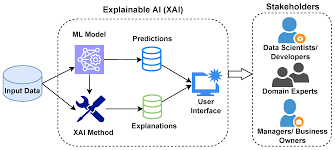
\includegraphics[width=0.65\linewidth]{assets/XAI.png}
	\caption{Explainable AI (XAI) layer integration within the automated diagnostic pipeline, illustrating the mapping of latent feature spaces to localized spatial heatmaps for clinical validation.}
	\label{fig:xai_in_action}
\end{figure}


\subsection*{Federated Learning Frameworks for Decentralized Thoracic Imaging}
\label{subsec:federated_learning}

Federated Learning (FL) represents a transformative decentralized optimization paradigm designed to facilitate collaborative, multi-institutional machine learning model development while guaranteeing complete local data sovereignty. In classical centralized deep learning frameworks, large-scale medical imaging repositories must be aggregated from multiple disparate clinical sites into a singular, central cloud repository or a unified computing infrastructure. This centralized architectural model introduces massive single-point-of-failure vulnerabilities, extreme network bandwidth consumption, and significant regulatory hurdles. 

Conversely, Federated Learning reverses this computational direction: rather than transmitting immense quantities of sensitive diagnostic imaging data over external networks to the centralized model, the abstract global model is transmitted directly to the decentralized institutional edge nodes. This foundational shift directly addresses the most critical hurdles in contemporary healthcare ecosystems, including strict patient privacy requirements, enterprise-grade data security protocols, legal liabilities, and the massive logistical burdens of cross-border medical dataset aggregation.

Within the high-stakes domain of clinical thoracic AI, datasets acquired across a multitude of independent hospitals, imaging centers, and regional health systems are fundamentally heterogeneous, geographically isolated, and legally protected[cite: 7, 10, 41]. Regulatory bodies enforce strict privacy statutes—such as the General Data Protection Regulation (GDPR) in the European Union and the Health Insurance Portability and Accountability Act (HIPAA) in the United States—which treat medical images and their associated metadata as highly sensitive Protected Health Information (PHI). 

Federated Learning provides a mathematically sound solution to these constraints by ensuring that raw patient data remains isolated behind institutional firewall structures throughout the entire lifecycle of model optimization[cite: 46]. The global model undergoes iterative optimization cycles by distributing parameter weights to individual clients, executing localized stochastic gradient descent loops entirely on edge hardware, and transmitting only abstract weight deltas or gradient updates back to a central orchestrating server. This collaborative process enables the underlying network to learn from massive, multi-institutional datasets of diverse patient distributions and varying scanner hardware configurations, which is critical for building a highly generalizable model capable of detecting rare, subtle lung abnormalities.

Federated Learning enhances clinical artificial intelligence development through several mechanisms:

\begin{itemize}
	\item \textbf{Complete Prevention of PHI Transmission:} Allowing diverse diagnostic centers to collaboratively train advanced deep networks without exposing, transmitting, or consolidating raw patient data.
	\item \textbf{Massive Global Generalizability and Scale:} Leveraging diverse datasets from distinct global populations, distinct geographic regions, and varying demographic slices, which directly prevents over-indexing on localized institutional distribution skews.
	\item \textbf{Significant Reduction of Data Breach Surfaces:} Mitigating systemic data breach risks and cyber-attacks by eliminating central honey-pot storage architectures, keeping sensitive information protected within local server environments.
	\item \textbf{Inherent Regulatory and Ethical Compliance:} Providing built-in compliance with evolving legal frameworks and data retention policies by minimizing data duplication and movement.
	\item \textbf{Continuous Edge-Driven Model Evolution:} Supporting lifelong and continuous learning patterns as edge institutions acquire new clinical imaging data during daily diagnostic workflows, without disrupting local institutional pipelines.
\end{itemize}

A multitude of aggregation strategies and architectural frameworks have been engineered to navigate the complex constraints of distributed medical imaging data. The foundational optimization baseline is \textit{Federated Averaging (FedAvg)}, where the central server initializes global model weights, distributes them to selected clients, and then computes a coordinate-wise weighted average of the local parameters based on the specific volume of data hosted at each institutional node after local optimization rounds. 

To stabilize convergence when dealing with severe non-IID client distributions, advanced aggregation algorithms like FedProx introduce proximal regularization terms to bound local parameter drift, while SCAFFOLD uses control variates to correct for localized client gradients. Furthermore, modern healthcare deployments implement security layers like Secure Aggregation (SecAgg) protocols based on cryptographic multi-party computation, alongside Differential Privacy (DP) techniques that add calibrated noise to local weight vectors to defend against reverse-engineering or model-inversion attacks. These privacy-preserving frameworks can also be paired with deep transfer learning, multi-task heads, and multi-modal feature fusion layers, allowing deep networks to optimize across distributed data streams while maintaining strong privacy guarantees. Figure~\ref{fig:federated_learning_pipeline} details the central-server approach to federated learning, illustrating the iterative parameter exchange loop between the global aggregator and the secure edge nodes.

\begin{figure}[H]
	\centering
	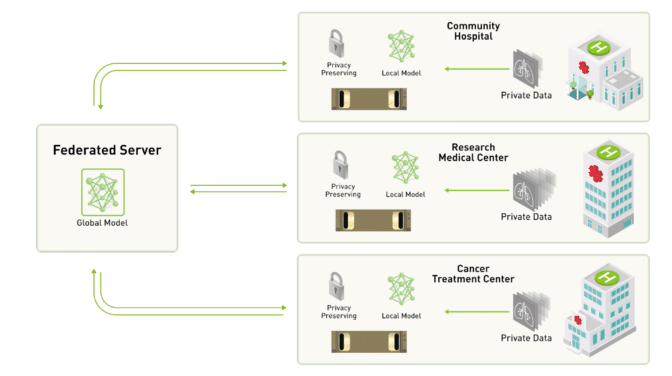
\includegraphics[width=0.8\linewidth]{assets/federated_learning.png}
	\caption{Centralized server architecture for federated learning, detailing the secure, iterative parameters exchange loop between the global orchestrator and localized institutional edge nodes.}
	\label{fig:federated_learning_pipeline}
\end{figure}

\section{Project Scope}
\label{sec:project_scope}

The fundamental scope of this research and development initiative centers on engineering, validating, and establishing an enterprise-grade, decentralized, and highly explainable medical computer vision ecosystem dedicated exclusively to multi-class thoracic pathology diagnosis. This advanced platform is structurally and algorithmically optimized to detect, classify, and spatio-temporally localize four highly prevalent, clinically severe, and socio-economically impactful thoracic conditions: acute pneumonia, Coronavirus Disease 2019 (COVID-19), chronic pulmonary tuberculosis (TB), and malignant lung cancer/chest masses. These conditions were strategically selected due to their massive contribution to global respiratory morbidity and mortality, the high risk of catastrophic clinical consequences if their initial radiological presentation is overlooked, and the immense structural variability they present across projectional and cross-sectional medical imaging modalities. By synthesizing advanced deep neural architectures with zero-trust decentralized optimization frameworks and post-hoc visual attribution models, this project scope explicitly establishes a robust, privacy-preserving machine learning diagnostic engine that can operate seamlessly across multi-institutional hospital networks.

The core technical boundary of this project is strictly defined by the integration, training, and fine-tuning of multi-modal deep learning models engineered to process two distinct clinical imaging streams. For the detection and differentiation of acute inflammatory and viral respiratory conditions (pneumonia and COVID-19), the system utilizes high-resolution projectional Chest X-ray (CXR) DICOM datasets, capturing fine-grained variations in alveolar and interstitial attenuation. For chronic infectious diseases and neoplastic lesions (tuberculosis, dense pulmonary masses, and lung cancer), the analytical pipeline is expanded to ingest and process high-contrast, cross-sectional chest Computed Tomography (CT) scans, enabling the extraction of multi-planar spatial features, volumetric nodule boundaries, and subtle morphological variations like edge spiculation or irregular calcifications. The machine learning pipeline is mathematically optimized to balance the trade-offs between diagnostic sensitivity and specificity, guaranteeing high recall to minimize false negative outcomes in clinical triage while maintaining precision to prevent downstream diagnostic bottlenecks and patient anxiety.

To guarantee seamless real-world deployability, abstract technological feasibility, and practical utility within active clinical environments, the backend diagnostic engine is natively wrapped inside a secure, low-latency, and web-based enterprise application interface. This front-end medical console is architected to allow non-technical healthcare practitioners, including front-line triage nurses, general physicians, emergency room technicians, and specialized thoracic radiologists, to securely ingest imaging files, execute distributed inference pipelines, and interact dynamically with the localized diagnostic outputs without requiring prior knowledge of deep learning mechanics, server configurations, or parameter tuning. While this cross-platform interface serves as a critical component for simulating real-world medical deployment and validating clinical integration, the primary focus, computational allocation, and academic scope of this project remain rigorously fixed upon the underlying mathematical formulations, decentralized federated optimization trajectories, model convergence stability under non-IID conditions, and the quantitative reliability of the explainable AI visualizations.

The functional boundaries and high-level architectural mandates of the system are categorized across four distinct, integrated operational vectors:

\begin{itemize}
	\item \textbf{Automated Multi-Class Thoracic Disease Identification:} Seamlessly processing heterogenous, multi-modal clinical image streams to perform differential classification across pneumonia, COVID-19, tuberculosis, and lung cancer/chest masses, effectively separating them from pristine normal baseline images.
	\item \textbf{Decentralized, Privacy-Preserving Collaborative Optimization:} Executing a secure, zero-trust federated learning protocol that orchestrates iterative parameter aggregation loops across distributed edge servers, strictly ensuring that protected health information (PHI) and raw patient images never exit local institutional firewalls.
	\item \textbf{Explainable Spatial Localization and Visual Justification:} Automatically coupling all deterministic classification outputs with high-fidelity, pixel-level attribution maps and self-attention weight heatmaps, explicitly highlighting the exact anatomical contours, parenchymal patches, or nodular boundaries that informed the network's predictive pathways.
	\item \textbf{Enterprise Web Deployment and Ingestion Architecture:} Constructing a secure web console featuring automated DICOM processing, smooth scaling across diverse hardware devices, and clean data visualizations tailored to match active clinical triage environments.
\end{itemize}

Crucially, the scope of this project is strictly defined by an assistive, clinician-in-the-loop operational philosophy and does \emph{not}, under any circumstances, aim to replace or supersede the definitive diagnostic judgment, clinical intuition, or legal accountability of professional medical practitioners or board-certified radiologists. Instead, the framework is meticulously engineered to function as an advanced, high-throughput second-opinion mechanism and triage assistant capable of reducing diagnostic oversights, mitigating human cognitive fatigue, and accelerating clinical turnaround times in high-volume emergency environments. 

Several technical boundaries are explicitly designated as out-of-scope for the current implementation phase to ensure absolute focus on the core machine learning and federated optimization objectives. The system is constrained to the four specified target conditions; the inclusion of other diffuse thoracic abnormalities (such as pneumothorax, chronic obstructive pulmonary disease, emphysema, or pleural effusions) falls entirely outside the project's current boundaries. Furthermore, while the federated learning layer is mathematically modeled and simulated to replicate a multi-hospital clinical network with severe statistical non-IID data distributions, the deployment scope is executed within distributed, multi-GPU simulated edge clusters rather than active, live-production hospital server backbones. Real-world institutional deployment across live physical hospital networks, real-time edge streaming, and expansion to handle non-thoracic disease modalities are deferred to future operational iterations, serving as logical continuations of this foundational architectural framework.

\begin{table}[htbp]
	\centering
	\caption{Project scope boundary matrix: Delineating technical inclusions, explicit exclusions, and target clinical metrics.}
	\label{tab:project_scope_matrix}
	\small
	\begin{tabularx}{\textwidth}{lXX}
		\toprule
		\textbf{Scope Category} & \textbf{Explicit Technical Inclusions} & \textbf{Explicit Technical Exclusions} \\
		\midrule
		\textbf{Target Pathologies} & Pneumonia, COVID-19, Pulmonary Tuberculosis (TB), and Lung Cancer/Chest Masses. & Pneumothorax, Emphysema, Pleural Effusions, Scoliosis, and Lung Nodules. \\
		\addlinespace
		\textbf{Imaging Modalities} & High-resolution projectional Chest X-rays (CXR) and cross-sectional chest CT scans. & Magnetic Resonance Imaging (MRI), Ultrasound, and Positron Emission Tomography (PET). \\
		\addlinespace
		\textbf{Data Protocols} & Zero-trust Federated Learning (FedAvg) using simulated non-IID distributed edge clients. & Live central cloud data pooling or live physical network integration into active EHR backbones. \\
		\addlinespace
		\textbf{Interpretability Layer} & Post-hoc visual attributions via Grad-CAM and self-attention rollout maps. & Automated clinical prescription generation or natural language therapy recommendations. \\
		\bottomrule
	\end{tabularx}
\end{table}

\section{Project Objectives} \label{sec:objectives}

The objectives of this project are centered around creating a reliable, accurate, and accessible diagnostic support system for lung tumor and chest diseases identification. The project aims to ensure that the system not only performs well in terms of machine learning metrics but also provides practical value to clinicians through usability, efficiency, and cost-effectiveness. Achieving clinical-level performance requires a well-defined set of goals that align both with technical constraints and real-world medical needs.

A primary objective is to develop a computer vision model capable of achieving high diagnostic performance. In particular, the system is designed to reach an accuracy above 90\% across its targeted conditions while maintaining a recall rate that minimizes the risk of missed fractures or tumors. Since false negatives can lead to severe clinical consequences, optimizing recall is essential for ensuring the safety and reliability of the system.

In addition to predictive performance, another major objective is to deliver an intuitive and engaging web interface that enables medical personnel to interact with the system easily. The interface should allow users to upload images, view results, and interpret highlighted regions without requiring technical expertise. Ease of use is critical for facilitating adoption in real clinical workflows, where time efficiency and clarity are important.

Operational efficiency is also a key objective. The system must be designed in a manner that minimizes computational overhead and reduces ongoing costs. This includes optimizing model size, using lightweight inference strategies where possible, and ensuring that the web application remains responsive even with limited hardware resources.

To summarize, the project seeks to meet the following objectives:

\begin{itemize}
	\item Achieve a diagnostic accuracy exceeding 90\% on lung tumor and chest diseases detection tasks.
	\item Maintain a high recall rate to reduce the likelihood of missed abnormalities.
	\item Provide a user-friendly, accessible, and engaging web interface suitable for non-technical clinical staff.
	\item Develop an efficient system that minimizes operational and computational costs.
\end{itemize}

Collectively, these objectives define the criteria by which the success of the project will be evaluated and guide the design decisions throughout development.

\section{Project Challenges}

Despite the remarkable progress achieved in recent years, medical image analysis remains a challenging field. The complexity of medical data, the critical nature of clinical decision-making, and the variability of imaging procedures introduce numerous obstacles that must be addressed to develop reliable and clinically applicable systems. The following subsections discuss the major challenges associated with medical image analysis, particularly in the context of chest disease detection using X-ray images and lung cancer detection using CT scans.

\subsection*{Limited Availability of High-Quality Medical Data}

One of the most significant challenges in medical image analysis is the limited availability of large, high-quality, and well-annotated datasets. Deep learning models generally require substantial amounts of labeled data to achieve high performance and robust generalization. However, obtaining medical images with accurate annotations is often difficult and expensive.

Medical image annotation requires the expertise of trained radiologists or medical specialists who must carefully examine each image and identify pathological findings. This process is time-consuming and resource-intensive. Furthermore, patient privacy regulations and ethical considerations often restrict the sharing of medical data between healthcare institutions, limiting the availability of publicly accessible datasets.

In the context of chest X-ray analysis, some diseases may occur infrequently, leading to severe class imbalance within datasets. Similarly, for lung cancer detection from CT scans, obtaining sufficiently large collections of confirmed malignant and benign cases can be challenging. These limitations can negatively affect model training and reduce diagnostic performance.

\subsection*{Variability in Image Acquisition}

Medical images are acquired using different imaging devices, protocols, and settings across hospitals and healthcare facilities. As a result, images may exhibit significant variations in quality, resolution, contrast, brightness, noise levels, and anatomical positioning.

Chest X-ray images obtained from different institutions may vary due to differences in machine manufacturers, patient positioning techniques, exposure settings, and image preprocessing procedures. Likewise, CT scans may differ in slice thickness, reconstruction algorithms, scanning protocols, and radiation dose levels.

Such variability can lead to distribution shifts between training and deployment environments. A model trained on data from one institution may experience performance degradation when applied to images acquired in another clinical setting. Ensuring robustness across diverse imaging conditions remains a major challenge for medical image analysis systems.

\subsection*{Image Noise and Artifacts}

Medical images frequently contain noise and artifacts that can obscure important anatomical structures and pathological findings. These imperfections may arise from patient movement, hardware limitations, acquisition errors, or environmental factors during image capture.

In chest X-ray imaging, artifacts such as medical devices, implants, external objects, and improper positioning can interfere with disease detection. CT scans may contain motion artifacts, beam-hardening effects, metal artifacts, and reconstruction-related distortions.

The presence of noise and artifacts can significantly reduce image quality and negatively affect the performance of automated detection systems. Consequently, effective preprocessing techniques, including image enhancement, denoising, and artifact removal, are often required before analysis.

\subsection*{Complexity of Disease Manifestations}

Many thoracic diseases exhibit highly variable visual characteristics, making automated detection particularly challenging. Diseases may present differently depending on their severity, progression stage, patient demographics, and coexisting medical conditions.

For example, pneumonia, tuberculosis, pulmonary edema, and COVID-19 may produce overlapping radiographic features in chest X-rays. Similarly, lung nodules observed in CT scans can vary considerably in size, shape, texture, density, and location. Some malignant nodules closely resemble benign abnormalities, increasing the difficulty of accurate classification.

Additionally, certain diseases may manifest as subtle changes that are difficult to detect even for experienced radiologists. Developing models capable of recognizing both obvious and subtle pathological patterns remains a critical research challenge.

\subsection*{Class Imbalance in Medical Datasets}

Medical datasets often suffer from class imbalance, where healthy cases significantly outnumber disease-positive cases or where some diseases occur much less frequently than others. This imbalance can lead machine learning models to favor majority classes during training.

For instance, in chest X-ray datasets, normal scans may constitute a large proportion of the available data, while rare diseases may only be represented by a small number of samples. Similarly, in lung cancer screening datasets, malignant nodules may be considerably less common than benign findings.

Class imbalance can result in poor sensitivity for detecting rare but clinically important conditions. Addressing this issue often requires specialized techniques such as data augmentation, oversampling, synthetic data generation, weighted loss functions, and balanced training strategies.

\subsection*{Interpretability and Explainability}

Healthcare professionals require transparency and trust when using artificial intelligence systems in clinical practice. Many state-of-the-art deep learning models function as black-box systems, producing predictions without providing clear explanations for their decisions.

In medical diagnosis, explainability is particularly important because clinicians must understand the reasoning behind automated recommendations before incorporating them into patient care decisions. A prediction without justification may not be sufficient in high-stakes medical environments.

To address this challenge, researchers employ explainable AI techniques such as saliency maps, Grad-CAM visualizations, attention mechanisms, and feature attribution methods. These approaches help identify image regions that contribute most strongly to model predictions, thereby improving transparency and clinical confidence.

\subsection*{Generalization and Robustness}

A medical image analysis system must perform reliably across different patient populations, imaging devices, healthcare institutions, and geographical regions. However, models trained on specific datasets may inadvertently learn dataset-specific characteristics rather than clinically meaningful features.

This issue can lead to reduced performance when models encounter unseen data during real-world deployment. Factors such as demographic differences, variations in disease prevalence, and differences in imaging protocols can all affect model generalization.

Ensuring robustness requires diverse training datasets, rigorous validation procedures, external testing across multiple institutions, and continuous performance monitoring after deployment.

\subsection*{Three-Dimensional Nature of CT Data}

Unlike chest X-rays, which provide two-dimensional projections, CT scans generate three-dimensional volumetric data. While this additional information improves diagnostic capabilities, it also introduces substantial computational and analytical challenges.

CT volumes may contain hundreds of slices for a single patient examination. Processing such large datasets requires considerable memory, storage capacity, and computational resources. Furthermore, accurately identifying lung nodules often requires analyzing spatial relationships across multiple slices.

Advanced techniques such as 3D convolutional neural networks, volumetric segmentation algorithms, and multi-view learning approaches are commonly employed to address these challenges. However, these methods generally demand greater computational complexity and longer training times.

\subsection*{Accurate Segmentation of Anatomical Structures}

Segmentation is a fundamental step in many medical image analysis pipelines. It involves identifying and isolating relevant anatomical structures such as lungs, airways, lesions, tumors, and nodules.

Accurate segmentation is particularly challenging when boundaries are unclear, tissues overlap, or pathological regions exhibit irregular shapes. In chest X-ray images, overlapping anatomical structures can complicate lung segmentation. In CT scans, tumors may have poorly defined margins or be attached to surrounding tissues.

Segmentation errors can propagate through subsequent analysis stages and adversely affect disease detection and classification performance. Therefore, robust segmentation algorithms remain an important area of ongoing research.

\subsection*{Clinical Validation and Regulatory Requirements}

Developing an accurate machine learning model is only one step toward clinical adoption. Medical image analysis systems must undergo extensive validation to demonstrate safety, reliability, and effectiveness in real-world healthcare environments.

Clinical validation typically involves testing models on large and diverse patient populations, comparing performance against expert radiologists, and assessing their impact on clinical workflows. Furthermore, healthcare technologies are subject to strict regulatory requirements and quality standards before deployment.

Meeting these regulatory and clinical validation requirements can be a lengthy and resource-intensive process, but it is essential for ensuring patient safety and maintaining trust in AI-assisted diagnostic systems.

\subsection*{Ethical and Privacy Considerations}

Medical image analysis systems operate on highly sensitive patient information. Protecting patient privacy and ensuring compliance with healthcare regulations are critical responsibilities throughout the development lifecycle.

Issues such as data security, informed consent, data ownership, and algorithmic bias must be carefully addressed. Models trained on non-representative datasets may exhibit reduced performance for certain demographic groups, potentially leading to inequitable healthcare outcomes.

Consequently, ethical AI development requires responsible data management practices, fairness assessments, transparency, and continuous evaluation to ensure that diagnostic systems benefit all patient populations.

\subsection*{Computational Resource Requirements}

Modern deep learning architectures used in medical image analysis often contain millions of trainable parameters and require substantial computational resources for training and inference. High-resolution chest X-ray images and volumetric CT scans further increase computational demands.

Training advanced models frequently requires powerful Graphics Processing Units (GPUs), large memory capacities, and extensive training times. These requirements may limit accessibility for smaller healthcare institutions and research groups with limited computational infrastructure.

Optimizing model efficiency while maintaining diagnostic accuracy remains an important challenge, particularly for deployment in resource-constrained clinical environments.

\section{Summary}
\label{sec:summary}

This chapter established the fundamental motivation, core medical context, and foundational technical architecture behind the development of an intelligent, decentralized, and highly transparent thoracic medical imaging platform. The rapid expansion of diagnostic imaging workloads within modern healthcare environments, combined with the extreme physiological subtlety of multi-class thoracic anomalies, has created an urgent, safety-critical requirement for enterprise-grade computer-aided diagnostic systems. Traditional radiographical interpretation processes are inherently vulnerable to human oversight caused by cognitive fatigue, subtle or overlapping pathological manifestations, and massive data distribution shifts induced by varying institutional imaging hardware and patient demographic skews.

To address these vulnerabilities, this chapter comprehensively explored the integration of advanced computer vision pipelines within clinical workflows, specifically targeting the detection and segmentation of highly infectious respiratory conditions and malignant neoplastic lesions. While deep learning architectures have demonstrated remarkable success in extracting high-level semantic abstractions from medical image grids, conventional centralized optimization paradigms face severe implementation barriers. Strict global data protection regulations and the risk of catastrophic data breaches legally restrict institutions from pooling sensitive patient records, which ultimately triggers model overfitting and prevents the development of generalized, clinically robust artificial intelligence models.

The rationale for the proposed platform directly resolves this technical and legal impasse by synthesizing state-of-the-art multi-scale deep neural networks with cutting-edge Explainable AI (XAI) pipelines and privacy-preserving Federated Learning (FL) aggregation strategies. This integrated design optimizes multi-class diagnostic sensitivity while providing pixel-level spatial attributions that map directly to peer-reviewed radiological criteria, allowing clinicians to confidently verify and audit the underlying decision-making logic. Simultaneously, the decentralized optimization framework enables secure, multi-institutional collaboration by transmitting only encrypted, abstract parameter updates over secure network layers, keeping raw patient records entirely localized and protected behind institutional firewalls.

Furthermore, the scope and technical objectives of this research were precisely defined to guide development toward real-world clinical viability. The architecture focuses on achieving maximum diagnostic sensitivity and localization accuracy for pneumonia, COVID-19, tuberculosis, and lung cancer across multi-modal image streams, while ensuring communication efficiency, robust edge-node security, and seamless clinical workflow integration. This chapter detailed the algorithmic and logistical challenges anticipated during development—such as severe statistical non-IID data skew, feature overlap, gradient drift, and adversarial inference risks—setting a clear benchmark for evaluating the platform's performance. In conclusion, this introductory analysis establishes the theoretical and practical foundation for an interpretable, privacy-preserving diagnostic platform, setting the stage for the detailed methodologies, experimental designs, and comparative performance evaluations presented in the subsequent chapters of this work.
\newpage
	
	%Chapter 2 Title page
	\vspace*{\fill} % Pushes content down from the top
	\thispagestyle{chapterpages}
	\begin{center} % Centers content horizontally
		\begin{minipage}{0.9\textwidth} % Creates a box for your text, adjust width as needed
			\centering % Centers text within the minipage
			{\color{RoyalBlue}\fontsize{30pt}{20pt}\bfseries\selectfont
				CHAPTER 2 
				\\[0.2cm] LITERATURE REVIEW
			}
		\end{minipage}
	\end{center}
	\vfill % Pushes content up from the bottom (equivalent to \vspace{\fill})
	\newpage
	
	% Chapter 2 content
	\chapter{Literature Review}
\pagestyle{default}
\thispagestyle{default}

In this chapter, a literature review is provided in project-related areas. To build the framework (X-Fed NeuroScan: Federated Learning with Explainable AI for Medical Image Classification), we need to get familiar with foundations of medical image analysis, deep learning-based classification techniques, and the challenges associated with handling sensitive clinical data. We also examine the principles and methodologies of Federated Learning (FL) as a privacy-preserving approach for multi-institutional model training, as well as Explainable AI (XAI) techniques that enhance model transparency and clinical trust. Additionally, this chapter reviews existing commercial medical imaging applications, related academic research, and publicly available datasets. Finally, we evaluate the tools, platforms, and frameworks that support the development of deep learning models, federated learning workflows, and explainable AI components.

The chapter is organized as follows:

\begin{itemize}
	\item Section 2.1: Medical image history and challenges, with subsections on bone fractures and chest diseases.
	\item Section 2.2: Explainable AI (XAI) in medical image detection.
	\item Section 2.3: Federated Learning (FL) in medical image detection.
	\item Section 2.4: Combined approaches integrating detection with XAI and FL.
	\item Section 2.5: Summary of related papers.
	\item Section 2.6: Similar commercial applications.
	\item Section 2.7: Summary of the chapter.
\end{itemize}

\section{Medical Image Diagnosis}

\textbf{Medical imaging} is the cornerstone of modern diagnosis, providing non-invasive visualization of the body’s interior using techniques like X-rays, Computed Tomography (CT), and Ultrasound. Due to the high volume and complexity of medical scans, interpretation is often time-consuming and subject to human variability. This process is increasingly enhanced by \textbf{Artificial Intelligence (AI)}, particularly \textbf{Computer Vision (CV)} and Deep Learning (DL) methods.

While traditional Deep Learning (DL) approaches have achieved high accuracy in radiological analysis for disease detection and bone fracture localization, their clinical deployment is significantly hindered. The primary issues stem from two critical needs: the strict requirement for \textbf{data privacy} and the \textbf{black-box nature} of AI decision-making. These barriers prevent the widespread, trustworthy adoption of powerful AI models in healthcare settings.

Consequently, the research focus has shifted toward specialized solutions: \textbf{Federated Learning (FL)}, a privacy-preserving paradigm, and \textbf{Explainable AI (XAI)}, a necessary component for model transparency. This work provides a systematic review of the state-of-the-art in these domains. It begins by examining advanced deep learning architectures, analyzing the role of FL in data collaboration, and reviewing XAI techniques.

We will first detail the related work in chest X-ray diagnosis and bone fracture detection. Subsequently, it will explore the use of XAI and FL specifically within these two application areas, identifying the gap that this research aims to bridge.

\subsection{Chest Diseases Detection}

The chest, encompassing the thoracic cavity, houses vital organs such as the lungs, heart, and major blood vessels, making it susceptible to various respiratory diseases that can be detected through imaging techniques like chest X-rays (CXR). CXR is a non-invasive, cost-effective diagnostic tool widely used for identifying abnormalities in lung tissue. We focus on four key categories for multiclassification: pneumonia, tuberculosis (TB), COVID-19, and normal (healthy) cases.

\begin{itemize} \itemsep 10pt
	\item \textbf{Pneumonia} is an inflammatory condition of the lung alveoli, often caused by bacterial, viral, or fungal infections, leading to fluid-filled sacs visible as opacities on CXR.
	\item \textbf{Tuberculosis} is a bacterial infection primarily caused by Mycobacterium tuberculosis, characterized by granulomas, cavities, or nodular infiltrates in the lungs, which can be chronic and contagious.
	\item \textbf{COVID-19}, caused by the SARS-CoV-2 virus, presents with ground-glass opacities, consolidations, and bilateral lung involvement on CXR, often progressing rapidly.
	\item \textbf{Normal cases} exhibit clear lung fields without pathological signs, serving as a baseline for comparison.
\end{itemize}
Accurate detection of these diseases via deep learning (DL) models on CXR images is crucial for timely intervention, especially in resource-limited settings \cite{ref8} \cite{ref9}.

\subsection{Target Diseases and Their Radiological Characteristics}

This study focuses on three major respiratory diseases that can be detected through chest X-ray imaging: pneumonia, COVID-19, and tuberculosis. These diseases represent significant public health concerns worldwide and are among the most commonly investigated conditions in computer-aided diagnostic systems. Although all three diseases affect the respiratory system, each exhibits distinct pathological characteristics and radiographic features that can assist clinicians in diagnosis. Understanding their symptoms and appearance in chest X-ray images is essential for accurate interpretation and effective disease detection.

\subsubsection*{Pneumonia}

Pneumonia is an inflammatory condition of the lungs that primarily affects the alveoli, the small air sacs responsible for gas exchange. The disease is commonly caused by bacterial, viral, or fungal infections, leading to the accumulation of fluid or pus within the affected lung tissue. Pneumonia remains one of the leading causes of respiratory-related morbidity and mortality, particularly among young children, elderly individuals, and immunocompromised patients.

Common symptoms of pneumonia include:

\begin{itemize}
	\item Persistent cough, often accompanied by mucus production.
	\item Fever and chills.
	\item Shortness of breath.
	\item Chest pain, especially during breathing or coughing.
	\item Fatigue and general weakness.
	\item Rapid breathing in severe cases.
\end{itemize}

In chest X-ray images, pneumonia typically appears as areas of increased opacity, commonly referred to as consolidations or infiltrates. These opacities occur due to the accumulation of inflammatory fluids within the alveoli, reducing the normal air content of the lungs. Depending on the severity and type of infection, the abnormalities may be localized to a single lobe (lobar pneumonia) or spread across multiple regions of the lungs. The affected areas generally appear whiter than healthy lung tissue, which normally appears dark due to the presence of air.

\subsubsection*{COVID-19}

Coronavirus Disease 2019 (COVID-19) is a highly contagious respiratory illness caused by the SARS-CoV-2 virus. Since its emergence, COVID-19 has posed substantial challenges to healthcare systems worldwide due to its rapid transmission and potentially severe respiratory complications.

The clinical presentation of COVID-19 varies considerably among patients, ranging from asymptomatic infections to severe respiratory failure. Common symptoms include:

\begin{itemize}
	\item Fever.
	\item Dry cough.
	\item Fatigue.
	\item Shortness of breath.
	\item Loss of taste or smell.
	\item Sore throat.
	\item Muscle and body aches.
	\item Headache.
\end{itemize}

Chest X-ray findings associated with COVID-19 often include bilateral lung abnormalities, particularly in the peripheral and lower lung regions. The disease commonly manifests as patchy or diffuse opacities that may affect both lungs simultaneously. As the infection progresses, these opacities may increase in size and density, resulting in widespread pulmonary involvement. Severe cases can demonstrate extensive bilateral infiltrates that significantly reduce the visibility of normal lung structures. Although chest X-rays are useful for evaluating disease progression, early-stage COVID-19 infections may not always produce clearly visible abnormalities.

\subsubsection*{Tuberculosis}

Tuberculosis (TB) is a chronic infectious disease caused by the bacterium \textit{Mycobacterium tuberculosis}. The disease primarily affects the lungs, although it can also spread to other organs. Tuberculosis remains a major global health concern, particularly in regions with limited healthcare resources.

The symptoms of pulmonary tuberculosis often develop gradually and may include:

\begin{itemize}
	\item Persistent cough lasting several weeks.
	\item Coughing up blood or blood-stained sputum.
	\item Chest pain.
	\item Fever.
	\item Night sweats.
	\item Unexplained weight loss.
	\item Fatigue and weakness.
	\item Loss of appetite.
\end{itemize}

Tuberculosis exhibits a wide range of radiographic appearances depending on the stage and severity of infection. In chest X-ray images, the disease frequently affects the upper lung regions and may appear as patchy infiltrates, nodular lesions, or areas of consolidation. Advanced cases can produce cavitary lesions, which are hollow spaces formed by tissue destruction within the lungs. Fibrosis and calcified granulomas may also be observed in chronic or healed infections. The diverse presentation of tuberculosis can sometimes complicate diagnosis, as certain imaging features overlap with those of other pulmonary diseases.

\subsubsection*{Comparative Radiological Characteristics}

Although pneumonia, COVID-19, and tuberculosis all affect the respiratory system and produce abnormalities in chest X-ray images, their radiographic patterns often differ. Pneumonia commonly presents as localized consolidations caused by fluid-filled alveoli, whereas COVID-19 typically produces bilateral and diffuse opacities that frequently involve the peripheral lung regions. Tuberculosis often demonstrates upper-lung involvement, nodular infiltrates, and cavitary lesions, particularly in advanced stages of the disease. Recognizing these characteristic imaging patterns is crucial for differentiating between conditions and supporting accurate clinical diagnosis.

\subsection{Related Work in Chest Diseases Multi-class Classification}
Interpreting Chest X-rays (CXRs) is vital for diagnosing various thoracic diseases like pneumonia and tuberculosis. Due to the subtlety of findings and high image volume, \textbf{Deep Learning (DL)} models have been widely adopted to automate diagnosis. These models, trained on large datasets, primarily focus on \textbf{multi classification} of different chest diseases. The following research examples showcase the success of various \textbf{Convolutional Neural Network (CNN)} architectures in achieving high accuracy in CXR analysis.

\begin{itemize} \itemsep 10pt
	\item The researchers Develop an automated Deep Neural Network (CNN) to classify Pneumonia, COVID-19, Tuberculosis, and No-findings from chest X-rays, addressing limitations in individual disease detection and small/biased datasets in prior studies.
	they Created a custom CNN architecture with 5 convolutional blocks (16-256 channels, ReLU activation, max-pooling), trained on split data (80\% training, 20\% testing). They Addressed heterogeneous data sources by preprocessing images (resizing to 300x300, denoising, normalization, filtering) to create a coherent dataset of 21,581 images from multiple Kaggle sources they achieve accuracy 98.72\% (using validation metrics) , Outperformed SOTA schemes like Venkataramana et al. (96.6\%) and Bhandari et al. (94.54\%), The study proved that a large diverse dataset is essential to achieve high multiclass accuracy and prevent overfitting, though class imbalance slightly reduced COVID-19 performance (96.27\% recall) \cite{ref10}.
	\item The researchers Develop a custom CNN model with soft attention to classify chest X-ray images into normal, COVID-19, pneumonia, and tuberculosis, while analyzing misclassifications through handcrafted features and statistical methods to improve clinical interpretability and diagnostic reliability. , Utilized transfer learning with pre-trained CNN models (VGG-19, ResNet-50, EfficientNet, DenseNet), trained on a balanced dataset split into training (70\%), validation (15\%), and testing (15\%) sets. They Preprocessed images via normalization, data augmentation (rotation, flipping, zooming), and resizing; applied SMOTE at the feature level to balance the originally imbalanced dataset from heterogeneous sources Best Modelis  ResNet-50 with 
	Accuracy:  97\% Compared to VGG-19 (95\%), DenseNet (91\%), EfficientNet (94\%) \cite{ref11}. 
	\item This study proposed a multi-level classification model using CNNs to differentiate COVID-19 from Tuberculosis (TB) and other Pneumonias based on CXR images. The primary challenge was addressing the severe data imbalance, specifically the scarcity of COVID-19 samples. The novelty involved combining data augmentation with the SMOTE technique to artificially balance the minority class. The system employed a two-stage process: first, classifying TB versus general Pneumonia, and second, sub-classifying the Pneumonia cases into COVID-19 and viral/bacterial types. This multi-level approach was designed to significantly reduce misdiagnosis between these similar lung diseases. The model achieved a high accuracy of 97.4\% for the TB/Pneumonia stage. The second stage achieved 88\% accuracy for bacterial/viral/COVID-19 classifications, demonstrating an overall 8–10\% improvement over existing methods \cite{ref12}.
	\item Additionally, a unified DL framework like CXR-MultiTaskNet used ResNet50 for joint disease localization and classification, incorporating thoracic diseases like pneumonia and TB, with an F1-score of 96.5\% through shared feature extraction \cite{ref13}.
	\item Another deep-learning pipeline classified chest X-ray images into normal, pneumonia, TB, and COVID-19 using a sequential CNN approach. Preprocessing steps such as grayscale conversion and normalization improved robustness, while transfer learning enhanced performance on limited data. VGG-16 achieved 95.9\%, DenseNet-161 reached 98.9\% for distinguishing COVID-19 from pneumonia, and ResNet-18 obtained 76\% for COVID-19 severity classification. The study demonstrates the effectiveness of multi-stage CNN models for automated COVID-19 screening from CXR images\cite{ref14}.
	\item A knowledge-distillation deep-learning model classified CXR images into COVID-19, pneumonia, TB, and normal using the RDD4 dataset. A deep CNN teacher network transferred its knowledge to a lightweight student model built in Keras/TensorFlow, preserving accuracy while reducing complexity. Data imbalance was addressed through augmentation. The distilled student model achieved 96.08\% accuracy, with high precision and recall, showing strong suitability for real-time, low-resource deployment\cite{ref15}.
	\item They develop a custom CNN model with soft attention to classify imbalanced chest X-ray images into normal, COVID-19, pneumonia, and tuberculosis, 
	the approach Designed COV-X-net19, a 16-layer CNN architecture (4 conv layers, 6 max-pooling, soft attention, dropout, dense with SoftMax), trained on split data (70\% training, 10\% validation, 20\% testing) with ablation studies for hyperparameter optimization (ReLU, Nadam optimizer, LR=0.001, batch=32) , the technique used preprocessed images via text removal (OCR+inpaint), morphological opening (3x3 kernel), CLAHE (ClipLimit=5.0, TileGridSize=3x3), histogram equalization. Best Model: COV-X-net19 with accuracy: 95.18\% Compared to 8 trans fer learning models (e.g., MobileNet at 82.96\%, VGG16 at 62.46\%), base CNN (89.96\%), and SOTA studies with similar multi-class setups (e.g., accuracies below 95\% in imbalanced scenarios) \cite{ref16}.
	\item A CNN-based system classified chest X-ray images into COVID-19, pneumonia, TB, and normal using over 21,000 images from three public datasets. The model used five convolutional blocks with preprocessing steps such as resizing, denoising, and normalization to handle heterogeneous sources. It achieved a high validation accuracy of 98.72\%, with strong per-class performance across all categories. The study shows that a carefully designed CNN can effectively support joint diagnosis of major chest diseases from CXR images \cite{ref17}.
	
\end{itemize}

\section{Explainable AI (XAI) in Medical Image Diagnosis}

Explainable AI (XAI) refers to techniques that make the decision-making process of AI models transparent and interpretable, addressing the "black-box" nature of DL models by providing insights into why a prediction was made. In this project, XAI is integrated using methods like Gradient-weighted Class Activation Mapping (GradCAM), which generates heatmaps highlighting regions in medical images (e.g., fracture lines in bone X-rays or opacities in CXR) that influenced the model's classification. This linkage enhances trust in diagnostics for both bone fractures and chest diseases, allowing clinicians to verify AI outputs against radiological features, reducing misdiagnosis risks, and facilitating model debugging.

\begin{figure}[htb]
	\centering
	\begin{minipage}{0.55\textwidth} % Adjust width as needed
		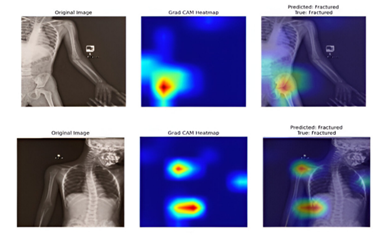
\includegraphics[width=\linewidth]{assets/bone_heatmap.png}
		\caption{Heatmap for bone}
		\label{fig:heatmap_bone}
	\end{minipage}
	\hfill % Adds horizontal space between minipages
	\begin{minipage}{0.40\textwidth} % Adjust width as needed
		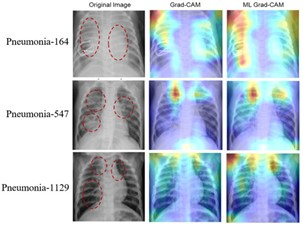
\includegraphics[width=\linewidth]{assets/pneumonia_heatmap.jpg}
		\caption{Heatmap for pneumonia detection}
		\label{fig:heatmap_pneumonia}
	\end{minipage}
\end{figure}

\subsubsection*{Related Papers on XAI For Bone Fracture Detection}
\begin{itemize} \itemsep 10pt
	\item Explainable AI has been increasingly integrated into medical imaging to ensure transparency  One study enhanced wrist fracture detection and classification by combining deep learning with XAI techniques, using saliency maps to highlight image regions that influenced predictions, thereby improving interpretability for clinicians. This work was presented in Enhancing Wrist Fracture Detection and Classification through Deep Learning and XAI (IEEE, 2024) \cite{ref18}.
	\item Another contribution focused on radiology, where machine learning models for bone fracture detection were augmented with XAI methods to visualize decision making processes. By providing interpretable outputs, the study bridged the gap between algorithmic accuracy and clinical usability. This was detailed in Enhancing Bone Fracture Detection in Radiology: A Machine Learning and Explainable AI Approach (IEEE, 2024) \cite{ref19}.
	\item Beyond fracture detection, interpretable machine learning has been applied to osteoporosis risk prediction. Comparative evaluations of predictive models were enriched with XAI analysis, allowing clinicians to understand how risk factors contributed to outcomes. This was reported in Interpretable Machine Learning for Osteoporosis Risk: A Comparative Evaluation of Predictive Models and XAI Analysis (IEEE, 2024) \cite{ref20}.
	\item Finally, advanced computational models have been proposed for predicting bone fracture healing and structural repair. XAI methods were employed to clarify how features influenced healing trajectories, supporting decision making in treatment planning. This was explored in XAI based Advanced Computational Models for Predictive Analysis of Bone Fracture and Structural Repair Healing Prediction (IEEE, 2024) \cite{ref21}.
	\item This study presents an Explainable AI system for humerus fracture detection utilizing deep learning models trained on 1,266 X-ray images from the MURA dataset. The researchers found that an ensemble of DenseNet architectures achieved a superior accuracy of 85\%, significantly outperforming standalone models like CNNs and VGGs. By integrating Saliency Maps and GRAD-CAM, the system visualizes specific fracture locations to ensure clinical interpretability and build trust with medical practitioners. This approach successfully combines high-performance automation with the necessary transparency for reliable orthopedic diagnosis \cite{ref22}.
	\item This study introduces a transparent AI framework for hand fracture detection using the YOLOv5m model trained on over 9,000 X-ray images. Optimized with specific preprocessing, the system achieved a superior 95.87\% accuracy, significantly outperforming architectures like Faster R-CNN in both speed and precision. The integration of Grad-CAM provides visual heatmaps with over 85\% localization accuracy, verifying that the model focuses on actual fracture lines rather than noise. This approach delivers a high-speed, interpretable diagnostic tool capable of enhancing clinical decision-making and trust \cite{ref23}. 
\end{itemize}

\subsubsection*{Related Papers on XAI For Chest Disease Multi-class Classification}
\begin{itemize} \itemsep 10pt
	\item This research introduces an Explainable AI (XAI) framework for the automatic detection, interpretation, and explanation of pulmonary diseases from chest radiographs (CXRs). The framework uses a transfer learning approach with a fine-tuned ResNet50 Convolutional Neural Network (CNN) trained on the COVID-CT and COVIDNet datasets. The Local Interpretable Model-agnostic Explanations (LIME) technique is employed to visually highlight the key regions in the CXR images that contribute most to the prediction. The developed system demonstrated strong performance, achieving high classification accuracy, reaching up to 97\% on the evaluated datasets. Validation confirmed that the model accurately focuses on clinically important features, thus assisting radiologists in early diagnosis and clinical decision-making\cite{ref24}.
	\item They develop XAI-TRANS, using inception-based transfer learning to classify CXR images for COVID-19, bacterial/viral pneumonia, and tuberculosis, addressing overlapping radiological features and black-box AI limitations by integrating improved U-Net segmentation and XAI tools the approach used is Utilized transfer learning with four pre-trained models (ResNet50, VGG19, VGG16, Inceptionv3), combined with an improved U-Net for lung segmentation to extract features, followed by XAI-TRANS for classification and explanation using Grad-CAM visualizations Technique Preprocessed images via resizing to 256*256 and normalization between 0 and 1fer learning models (e.g., MobileNet at 82.96\%, VGG16 at 62.46\%), base CNN (89.96\%), and SOTA studies with similar multi-class setups (e.g., accuracies below 95\% in imbalanced scenarios) the Best Model is XAI-TRANS (with and Grad-CAM) with accuracy: 97\% (overall classification accuracy) and 98\% precision, outperforming traditional DL methods by 4.75\% through XAI integration \cite{ref25}. 
	\item A survey reviewed over 200 papers on XAI in DL-based medical image analysis, emphasizing visual explanations for chest radiography to build clinician confidence\cite{ref26}.
	\item Additionally, an XAI-integrated DL framework for multiclass lung disease classification, targeting five classes: viral pneumonia, bacterial pneumonia, COVID-19, tuberculosis, and normal. It evaluates various DL architectures, including CNNs, hybrids, ensembles, transformers, and Big Transfer, with hyperparameter tuning and stratified 5-fold cross-validation to ensure robust performance. The Xception model, enhanced with transfer learning, emerges as the top performer, achieving 96.21\% accuracy by focusing on discriminative features in lung region\cite{ref27}.
	\item They built a lightweight CNN (5 convolutional layers) to classify chest X-rays into four classes: COVID-19, Pneumonia, TB, Normal. They applied Grad-CAM, LIME, and SHAP to generate visual explanations of model decisions, validating them with radiologists. The dataset was 7,132 public CXR images from three sources, with class imbalance handled by stratified batching. The model achieved a 10-fold cross-validation average test accuracy of 94.31\% ± 1.01\%, and they reported strong precision, recall, and F1\cite{ref28}.
\end{itemize}

\section{Federated Learning}

Federated Learning (FL) is a decentralized ML approach where models are trained collaboratively across multiple devices or institutions without sharing raw data, preserving privacy through local updates aggregated centrally. In medical imaging like bone X-rays and CXR classification, FL is used to train on distributed datasets from hospitals, mitigating data silos and complying with regulations like GDPR or HIPAA. It involves clients training on local data, sending model weights to a server for aggregation (e.g., via FedAvg), and is quickly implemented for real-time applications, reducing communication overhead while handling heterogeneous data.

\begin{figure}[htb]
	\centering
	\begin{minipage}{0.45\textwidth} % Adjust width as needed
		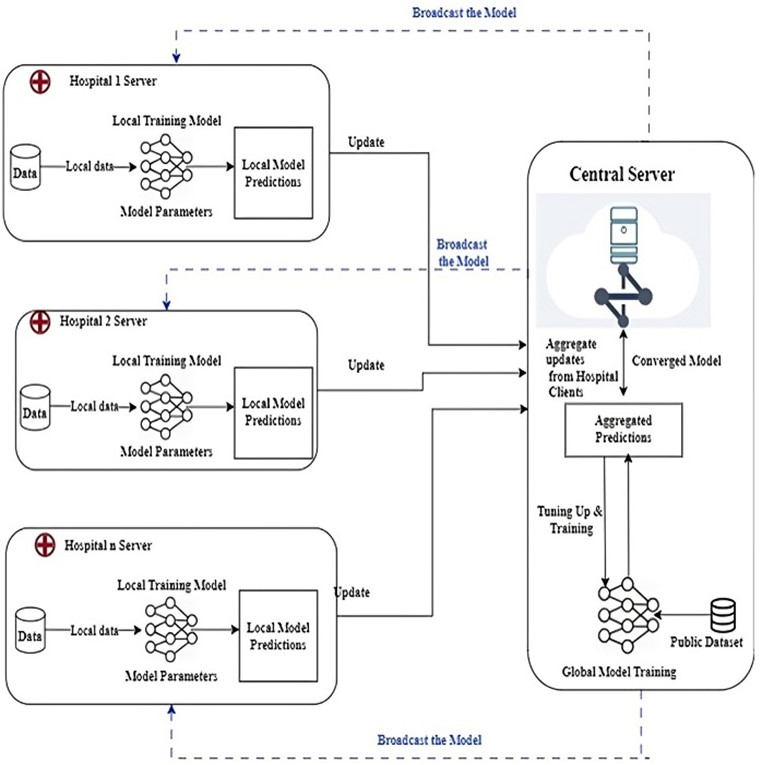
\includegraphics[width=\linewidth]{assets/federated1.jpg}
	\end{minipage}
	\hfill % Adds horizontal space between minipages
	\begin{minipage}{0.45\textwidth} % Adjust width as needed
		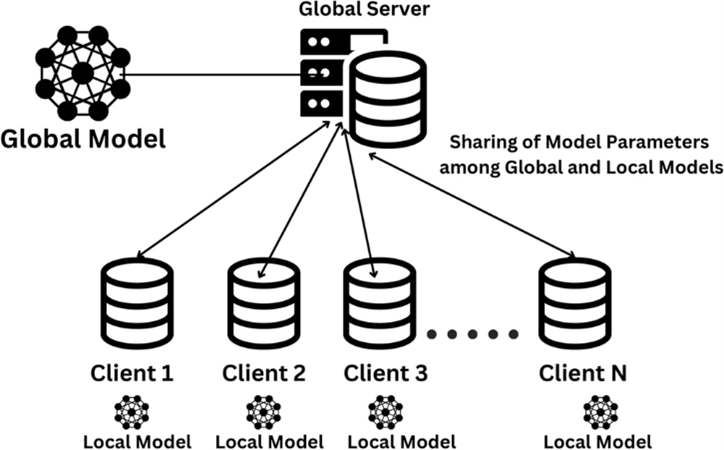
\includegraphics[width=\linewidth]{assets/federated2.png}
	\end{minipage}
	% Add more minipages for additional figures
	\caption{FL-Based efficient framework for smart healthcare sector}
	\label{fig:combined}
\end{figure}

\subsubsection{Related Papers on FL For Chest X-ray Disease Multi-class Classification}
\begin{itemize} \itemsep 10pt
	\item This study addresses the primary challenge in applying Federated Learning to chest X-ray analysis, which is the significant non-IID data distribution between adult and pediatric cohorts from different institutions. Analyzing over 400,000 radiographs, the research showed that conventional FL struggles to maintain consistent performance, particularly with the challenging pediatric dataset. The authors proposed enhancing FL by integrating general-purpose Self-Supervised Learning representations, using the DINOv2 model as a robust initialization.vThe new SSL-equipped framework proved highly effective, achieving an improvement exceeding 20\% in the AUC metric for pneumonia diagnosis in the difficult pediatric cases. This validates that readily available SSL models provide a practical and scalable solution for enabling FL in diverse healthcare settings while preserving data privacy\cite{ref33}.
	\item This study focuses on using federated learning (FL) for the accurate and privacy-preserving diagnosis of pediatric pneumonia via chest X-ray classification. Traditional machine learning approaches face significant challenges related to centralizing sensitive medical data, which risks patient privacy and security. FL addresses this by enabling collaborative model training across different institutions while ensuring the raw patient data remains local and secure. The researchers specifically tackled the common problem of data heterogeneity, which typically compromises classification accuracy in real-world clinical settings. They proposed an improved FL method utilizing "two-end control variables," modifying the loss function on the client side and adding momentum on the server. This novel approach successfully enhanced performance, achieving an average accuracy of 98\% and demonstrating an approximate 2\% improvement over existing federated learning algorithms. \cite{ref33}.
	\item Artificial Intelligence for lung disease detection is limited by major privacy concerns due to the need to centralize sensitive patient data (X-ray and CT scans). To overcome this, the paper proposes a decentralized Federated Transfer Learning (FTL) system, which enables effective collaborative model training without ever pooling raw data. This approach leverages federated learning's privacy features and the efficiency of transfer learning to train models on limited local datasets. The study evaluated four methods using the ResNet-50 model, confirming FTL as the most effective method for high accuracy. Specifically, the resulting accuracies were: Centralized (87.95\%), Transfer (88.04\%), Federated (87.55\%), and FTL (89.96\%) \cite{ref34}.
	\item A federated learning framework distinguished COVID 19 from four other chest diseases (lung cancer, TB, pneumothorax, pneumonia) plus normal using chest X rays from multiple hospitals. They used three pre trained models (DenseNet 169, VGG 16, VGG 19) and applied SMOTE to mitigate class imbalance. The aggregated system (using DenseNet 169) achieved 98.45\% accuracy, Grad CAM was used for model explainability, and their decision making client selection strategy reduced communication overhead significantly \cite{ref35}.
\end{itemize}

\section[Combined Approaches]{Combined Approaches: Medical Image Diagnosis with XAI and Federated Learning}

Integrating XAI and FL in medical image diagnosis combines privacy with interpretability, enabling collaborative training on bone X-rays and CXR while explaining predictions, with potential for broader medical domains. This section details key papers that merge these elements.

\subsection*{Related Papers on Combined Approaches for Chest Diseases Detection with XAI and Federated Learning}
\begin{itemize} \itemsep 10pt
	\item A Federated Learning Based Real Time Ensemble Model with Explainable AI Framework for an Efficient Diagnosis of Lung Diseases. It is FLEM-XAI, a privacy-preserving FL framework with XAI for real-time lung disease diagnosis from CXR, using FedAvg for decentralized training across hospitals without data sharing. It ensembles pre-trained models (InceptionV3, Conv2D, VGG16, ResNet-50) trained locally, aggregated centrally, and incorporates XAI via SHAP for feature importance and GradCAM for heatmaps highlighting affected lung areas. Results show ResNet-50 achieving 95.5\% overall accuracy (97.72\% COVID-19, 95.42\% pneumonia, 93.17\% TB), outperforming centralized models in bandwidth efficiency and maintaining convergence \cite{ref37}.
	\item This study introduces FLPneXAINet, a framework that securely predicts pneumonia from Chest X-ray (CXR) images by integrating Federated Learning (FL), Deep Learning (DL), and Explainable AI (XAI) to overcome data privacy issues. The method utilized an 8,402-image Kaggle dataset, which was augmented using a CycleGAN network, and then features were extracted via pre-trained DL models and four Ensemble DL (EDL) models. Feature optimization was performed using RFE, ANOVA, and RF to select the most relevant features, which were then classified by various machine learning models in an FL environment. The EDL network achieved the best results in the FL environment, with a high accuracy of 97.61\%, and was validated using XAI techniques (LIME and Grad-CAM). The full performance metrics were: F1 score 98.36\%, recall 98.13\%, and precision 98.59\%, offering a robust solution for healthcare professionals \cite{ref38}.
	\item A secure lung cancer prediction used mapreduce blockchain FL with XAI, ensuring interpretability in federated settings \cite{ref39}.
\end{itemize}

\section{Summary of Related Papers}
\renewcommand{\arraystretch}{1.2}
\begin{center}
	
	
	\begin{longtable}{|p{1cm}|p{1.5cm}|p{2cm}|p{1.8cm}|p{5cm}|p{1.2cm}|}
		\caption{Summary of related papers.} \\
		\hline
		\textbf{Focus Area} & \textbf{Sub-category} & \textbf{Model} & \textbf{Dataset} & \textbf{Result} & \textbf{Ref. Num.} \\ \hline % 
		Bones & General & Custom CNN and transfer learning & \textbf{FracAtlas} & The custom CNN achieved superior performance with 95.96\% accuracy, significantly outperforming the transfer learning models (EfficientNetB0, MobileNetV2, ResNet50) which only managed between 65\% and 67\% accuracy. & [1] \\ \hline
		
		Bones & General & YOLOv11 was developed and benchmarked against \textbf{Faster R-CNN} and SSD. & --- & YOLOv11 achieved superior performance with 96.8\% mAP and 95.14\% accuracy, significantly outperforming Faster R-CNN (87.5\% mAP) and SSD (82.9\% mAP) in both real-time fracture detection and localization. & [1] \\ \hline
		
		Bones & General & YOLOv11 was developed and benchmarked against Faster R-CNN and SSD. & --- & YOLOv11 achieved superior performance with 96.8\% mAP and 95.14\% accuracy, significantly outperforming Faster R-CNN (87.5\% mAP) and SSD (82.9\% mAP) in both real-time fracture detection and localization. & [1] \\ \hline
		
		Bones & General & EfficientNet-B6 & FracAtlas & The EfficientNet-B6 model achieved a 96.83\% testing accuracy & [3] \\
		\hline
		Bones & General & Custom CNN & ------ & The model achieved a classification accuracy of 92.44\% & [4] \\
		\hline
		Bones & General & SVM, k-NN, Naïve Bayes & -------- & Support Vector Machine (SVM) classifier achieved the highest accuracy, with a classification rate of 98\%. & [5] \\
		\hline
		Bones & General & Custom CNN & & Accuracy: 89.865\% (Approx. 90\%), Specificity: 89.90\% & [6] \\
		\hline
		Bones & General & Custom CNN & MURA dataset & Testing Accuracy: 99.79\% (at epoch 13). & [7] \\
		\hline
		Bones & XAI & MobileNetV3 style convolutional blocks with self-attention layers. & NEU Surface Defect Database, MVTec AD (Anomaly Detection), Severstal Steel Defect Dataset & proposed EdgeViT-Slim achieved 96.0\% accuracy, 0.953 F1 score, and 85 FPS on industrial defect datasets, outperforming baselines with far fewer parameters & [18] \\
		\hline
		Bones & XAI & ResNet-50, Faster R-CNN, and Mask R-CNN with Grad-CAM explainability & MURA & achieving 83\% classification accuracy (ResNet-50) & [19] \\
		\hline
		Bones & XAI & Random Forest, SVM, and KNN & MURA & Random Forest classifier achieved the best performance with 95\% accuracy, 93\% precision, and 0.96 F1-score, outperforming SVM (91\%) and KNN (88\%) & [20] \\
		\hline
		Bones & XAI & Logistic Regression, Random Forest, XGBoost, AdaBoost, LightGBM, and Gradient Boosting & custom multi-center clinical osteoporosis dataset (1,250 records) & ensemble model achieved the best performance with 90.82\% accuracy, 100\% precision, 81.63\% recall, and 89.99\% F1-score & [21] \\
		\hline
		Bones & XAI & (CNN, VGG, DenseNet) and found that Ensemble-2 (combining DenseNet121 and DenseNet169) & MURA dataset & The Ensemble-2 model achieved the highest accuracy of 85\% and an F1 score of 0.79. Additionally, the integration of Explainable AI (Grad-CAM and Saliency Maps) & [22] \\
		\hline
		Bones & XAI & YOLO, Faster R-CNN, & ------- & YOLOv5m (Best Performer) Achieved a Pointing Game Accuracy of $>85$\%, meaning Grad-CAM heatmaps consistently aligned with the ground truth fracture locations. & [23] \\
		\hline
		Bones & FL & DenseNet161 & & Federated Learning (FedAvg): The 5-node FedAvg model achieved the best performance with 91\% accuracy. Centralized Training: The centralized DenseNet161 model achieved 89.6\% accuracy. & [29] \\
		\hline
		Bone & FL & Local ML Models (Client-side), Federated Learning Frameworks (Server-side) & -- & Highest accuracy of 94.4\% (FL+VGG16 with augmentation) for binary classification. & [30] \\
		\hline
		Bones & FL & EfficientNet V2 (implemented within an Adaptive Federated Learning framework) & --- & federated methods lagged slightly behind the 96–98\% accuracy achieving near-centralized performance of up to 98.6\% using EfficientNetV2 & [31] \\
		\hline
		Bones & Combined & SemFedXAI (a framework combining Semantic Web technologies and Federated Learning & ------ & The SemFedXAI framework achieved the highest predictive accuracy at 85.3\%, outperforming standard Federated Learning (73.5\%) and other baselines. It also demonstrated superior explainability, scoring 0.85 in feature identification accuracy & [36] \\
		\hline
		Chest & General & Custom CNN & Kaggle \& IEEE & The model achieved 98.72\% overall accuracy across all classes. Recall per class: Pneumonia 99.66\%, No-findings 99.35\%, Tuberculosis 98.10\%, COVID-19 96.27\%. & [10] \\
		\hline
		Chest & General & & Kaggle & Accuracy: 97\% (using Resnet-50) VGG-19 (95\%), DenseNet (91\%), EfficientNet (94\%) & [11] \\
		\hline
		Chest & General & Custom CNN & Kaggle & TB vs Pneumonia classification: 97.4\% accuracy; COVID-19 vs viral/bacterial pneumonia vs (other pneumonia types) classification: 88.0\% accuracy & [12] \\
		\hline
		Chest & General & Custom CNN & VinDr-CXR & Classification Accuracy = 96.8\% (from micro-F1 $\approx$ 0.968) Localization Accuracy $\approx$ 85\% (IoU $\approx$ 0.851) & [13] \\
		\hline
		Chest & General & VGG16, DenseNet-161 and ResNet-18 & Custom clinical dataset collected and labeled & Normal/Pneumonia/TB/ COVID-19 classification (via VGG-16): 95.9\% . Normal/Pneumonia/COVID-19 classification (via DenseNet-161): 98.9\% . COVID-19 severity classification (via ResNet-18): 76.0\% . & [14] \\
		\hline
		Chest & General & Custom CNN & Kaggle & 97\% average accuracy (with precision $\approx$ 94\% and recall $\approx$ 97\%) for the full classification task. & [15] \\
		\hline
		Chest & General & Custom CNN and VGG-16 & Kaggle \& public dataset from Github & The COV-X-net19 achieves 95.18\% , MobileNet :  82.96\%, VGG16 : 62.46\% and  base CNN : 89.96\% . & [16] \\
		\hline
		Chest & General & DenseNet201, ResNet152V2 & IEEE & The model achieved superior performance with a test accuracy of 98.87\%, outperforming the individual base models (DenseNet201 and ResNet152V2) and demonstrating robust multi-class classification capabilities. & [17] \\
		\hline
		Chest & XAI & Explainable Framework based on DenseNet-201 & -- & The proposed explainable DenseNet-201 model achieved a high classification accuracy of 98.08\%, while also providing visual explanations (Grad-CAM) to build trust and interpretability for clinical diagnosis. & [24] \\
		\hline
		Chest & XAI & CNN and Vision Transformer & Kaggle & XAI-TRANS achieves accuracy: 97\% and 98\% precision & [25] \\
		\hline
		Chest & XAI & Review of various Deep Learning models and XAI techniques (e.g., Grad-CAM, LIME) & Survey of medical image analysis studies & & [26] \\
		\hline
		Chest & XAI & Custom CNN with Grad-CAM and LIME & -- & The proposed Custom CNN model achieved a high classification accuracy of 98.41\%, with XAI techniques successfully highlighting the critical image regions used for diagnosis, thereby improving model interpretability. & [27] \\
		\hline
		Chest & XAI & Ensemble of DenseNet201, InceptionResNetV2, Xception with Grad-CAM++ & Kaggle \& IEEE & The proposed deep learning ensemble achieved a superior average classification accuracy of 98.97\%, with XAI visualizations providing clinically plausible explanations for the model's decisions across all disease classes. & [28] \\
		\hline
		Chest & FL & Federated Learning (FedAvg) with a ResNet-based backbone and a novel age de-biasing loss function. & Multi-institutional chest X-ray datasets & The proposed de-biased FL model achieved an AUC of 89.7\%, outperforming the standard FL model (AUC of 86.2\%) and demonstrating significantly improved fairness and accuracy across different age groups. & [32] \\
		\hline
		Chest & FL & Federated Averaging (FedAvg) algorithm with a DenseNet-121 architecture as the core CNN model. & Chest X-ray images from multiple clients & The federated DenseNet-121 model achieved a test accuracy of 96.7\% and an F1-score of 95.8\%, matching the performance of a model trained on centralized data while preserving privacy. & [33] \\
		\hline
		Chest & FL & Federated Transfer Learning using a pre-trained ResNet-50 model, fine-tuned collaboratively across sites. & Collection from Kaggle & The federated transfer learning model achieved a classification accuracy of 96.3\% for detecting various lung diseases, significantly outperforming models trained on single, isolated datasets. & [34] \\
		\hline
		Chest & FL & A custom Federated Learning framework using a specialized Composite-DenseNet & -- & The DMFL\_Net framework achieved a high overall classification accuracy of 98.21\% and a precision of 98.14\%, demonstrating superior performance for multi-disease classification in a federated setting. & [35] \\
		\hline
		Chest & Combined & A Federated Learning-based Real-Time Ensemble Model combining multiple CNNs (VGG16, ResNet) with XAI techniques like Grad-CAM. & Kaggle & The FLEM-XAI ensemble model achieved accuracy of 99.4\% for multi-class lung disease classification. & [37] \\
		\hline
		Chest & Combined & A Federated Deep Learning framework using a custom CNN architecture integrated with XAI methods such as LIME and SHAP for model interpretation. & Chest X-ray images from distributed clients & The proposed FLPneXAINet framework achieved a high accuracy of 98.7\% in detecting pneumonia from chest X-rays & [38] \\
		\hline
		Chest & Combined & A Secure Framework using MapReduce, Blockchain-based Federated Learning, and XAI with a DenseNet-201. & Multi-source CT scan datasets & The secure federated learning model achieved an exceptional accuracy of 99.8\% for lung cancer prediction, leveraging blockchain for security and XAI for providing transparent, interpretable results. & [39] \\ \hline
	\end{longtable}
\end{center}

\section{Datasets Utilized in the Project}

\begin{table}[h]
	\centering
	\caption{Summary of Datasets Used in the Project}
	\label{tab:datasets}
	\renewcommand{\arraystretch}{1.3}
	\begin{tabular}{|p{3cm}|p{2cm}|p{7.5cm}|p{2.5cm}|}
		\hline
		\textbf{Dataset Name} & \textbf{Domain} & \textbf{Class Distribution / Description} & \textbf{Total Images} \\
		\hline
		FracAtlas & Bone &
		Fractured (1707), Hand (3487), Hardware (210), Hip (796), Leg (5293), Shoulder (796) &
		9,383 \\
		\hline
		COVID-19 \& Pneumonia \& Tuberculosis with Normal \& Non-X-ray &
		Chest &
		COVID-19 (\num{3616}), Normal (\num{5688}), Pneumonia (\num{4861}), Tuberculosis (\num{3453}) &
		\num{17618} \\
		\hline
		Chest X-ray Dataset for Lung Segmentation &
		Chest &
		Annotated chest X-ray images for lung segmentation tasks &
		\num{6106} images with corresponding \num{6106} masks \\
		\hline
		Random Images for Image Classification &
		General &
		Unlabeled random images used for general image classification experiments &
		\num{9958} \\
		\hline
		MURA &
		Bone &
		Elbow (1,912), Finger (2,110), Hand (2,185), Humerus (727), Forearm (1,010), Shoulder (3,015), Wrist (3,697) &
		40,561 images (14,656 studies) \\
		\hline
	\end{tabular}
\end{table}



\section{Similar Commercial Applications}

Several commercial applications leverage AI for medical image diagnosis, providing tools for clinicians to detect conditions like bone fractures and chest diseases. These applications often use DL models for classification but may lack advanced XAI or FL features for interpretability and privacy. Below, we discuss some notable examples.

\subsection{Aidoc (aiOS™)}
Aidoc is a leading clinical AI software company that utilizes its proprietary aiOS™ platform to deliver high-performance AI solutions for medical imaging interpretation and workflow optimization. The platform automatically analyzes medical scans, prioritizing critical findings like stroke, pulmonary embolism, and intracranial hemorrhage, and then notifies care teams in real-time. By integrating seamlessly with existing systems like EHR and PACS, Aidoc's solutions help radiologists streamline workflows, enhance diagnostic accuracy, and accelerate time-to-treatment for patients with acute conditions across radiology, cardiology, and neurovascular specialties.
\begin{figure*}[h]
	\centering
	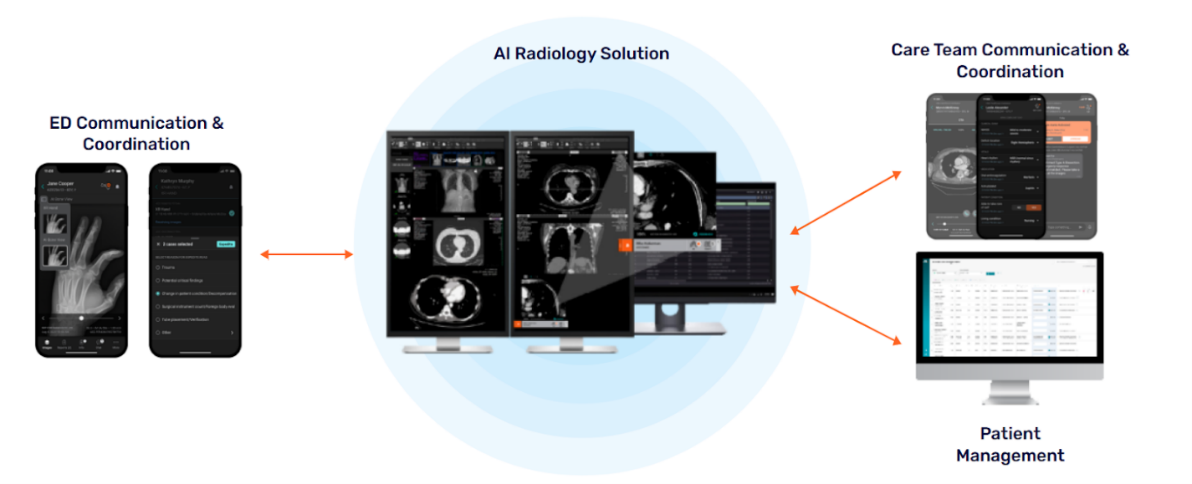
\includegraphics[width=0.5\linewidth]{assets/aidoc.png}
\end{figure*}

\subsection{Viz.ai (Viz.ai One®)}
Viz.ai is a leading AI-powered care coordination platform focused on transforming time-sensitive medical care by accelerating diagnosis and treatment decisions. The Viz.ai One® platform features multiple FDA-cleared AI algorithms that analyze imaging data, including CT scans and EKGs, to detect suspected diseases like stroke and pulmonary embolism. Crucially, it then uses real-time alerts and communication tools to instantly connect multidisciplinary care teams on mobile and desktop devices, ensuring the patient receives the necessary intervention as quickly as possible.
\begin{figure*}[h]
	\centering
	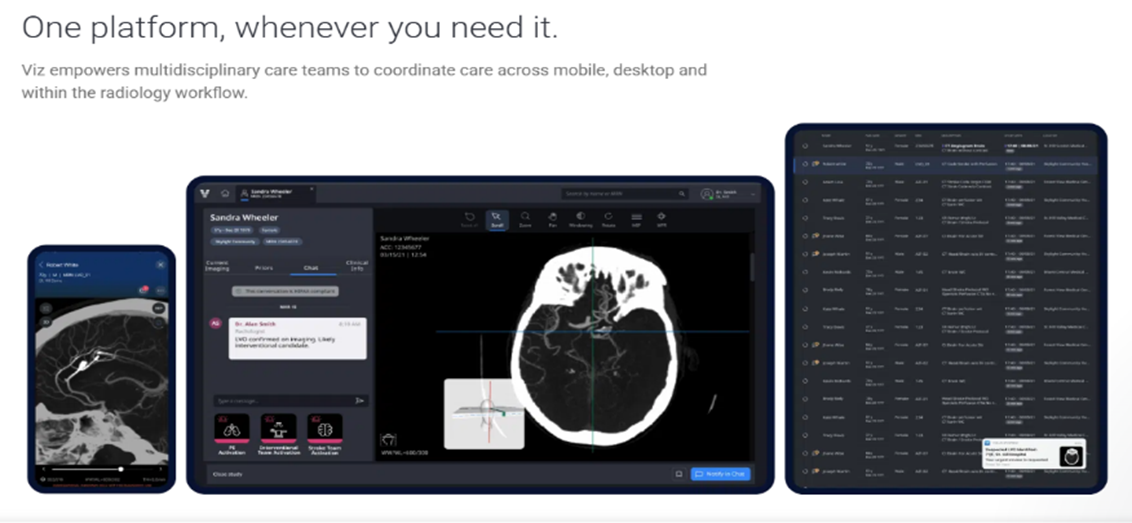
\includegraphics[width=0.5\linewidth]{assets/vizai.png}
\end{figure*}

\subsection{Qure.ai (qXR, qCT)}
Qure.ai specializes in developing deep learning algorithms for affordable and accessible diagnostics, with a strong presence in global health initiatives. Their core products, qXR (for chest X-rays) and qER/qCT (for head and lung CTs), use AI to detect and quantify abnormalities, including tuberculosis, lung nodules, and critical trauma findings. By analyzing scans with high accuracy in minutes, Qure.ai’s solutions assist radiologists in early disease detection, risk stratification, and provide essential diagnostic support, especially in areas with limited access to specialists.
\begin{figure*}[h]
	\centering
	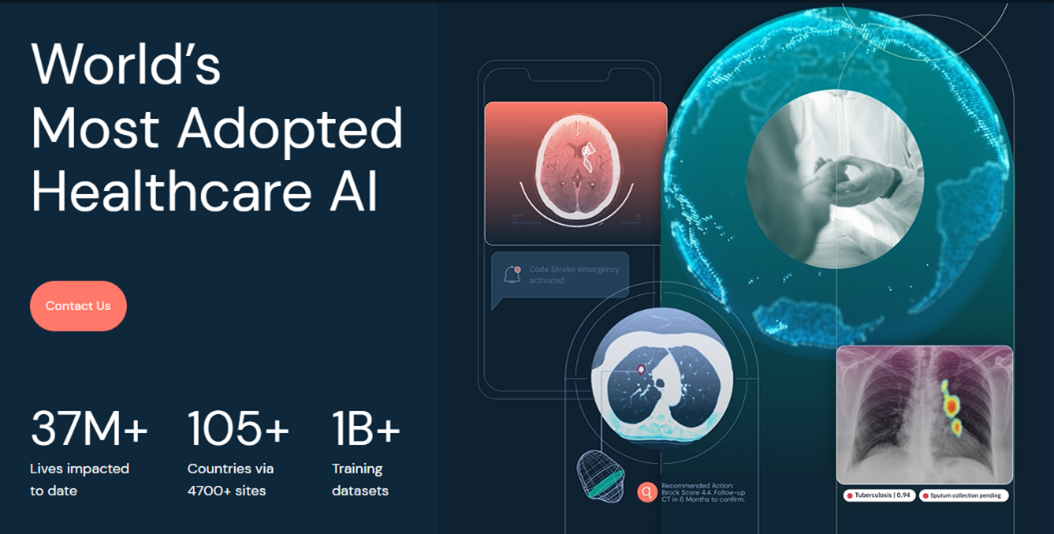
\includegraphics[width=0.5\linewidth]{assets/qure.png}
\end{figure*}

\subsection{Harrison.ai}
Harrison.ai, through its partnership with the I-MED Radiology Network 
(Annalise.ai), offers comprehensive, decision-supported AI tools designed to raise the standard of patient care and combat capacity limits. Their advanced AI solutions for Chest X-ray (CXR) and Non-contrast Head CT (CTB) are designed to detect a massive number of potential findings (often over 100) within seconds. By acting as a 'co-pilot' for clinicians, their AI solutions flag emergent and incidental findings, helping to reduce stress from chaotic worklists and significantly improving both diagnostic accuracy and efficiency.

\subsection{Lunit (Lunit INSIGHT, Lunit SCOPE)}
Lunit is a global leader in medical AI software with a singular mission to conquer cancer through cutting-edge technology. The company's solutions, including the Lunit INSIGHT suite for cancer screening (especially mammography and chest X-ray) and the Lunit SCOPE platform for precision oncology, transform complex clinical data into clear, actionable insights. By delivering highly accurate diagnostic results and extracting intelligence from tissue images to predict treatment response, Lunit empowers earlier detection and more precise treatment decisions across the entire cancer care continuum.

\section{Summary}

In this chapter, we presented the background on bone fractures and chest diseases as initial focus areas for medical image diagnosis, emphasizing multiclassification. We discussed similar commercial applications, reviewed related works on detection using DL for each domain, explainable AI techniques like GradCAM for interpretability (with potential image insertions for heatmaps), federated learning for privacy-preserving training, and combined approaches integrating these elements. We also evaluated tools for development. These insights form the foundation for our extensible project's development, highlighting gaps in interpretability and data privacy that our system aims to address for bone fracture detection, chest disease detection, and future expansions. \newpage
	
	%Chapter 3 Title page
	\vspace*{\fill} % Pushes content down from the top
	\thispagestyle{chapterpages}
	\begin{center} % Centers content horizontally
		\begin{minipage}{0.9\textwidth} % Creates a box for your text, adjust width as needed
			\centering % Centers text within the minipage
			{\color{RoyalBlue}\fontsize{30pt}{20pt}\bfseries\selectfont
				CHAPTER 3 
				\\[0.2cm] PROPOSED MODELS
			}
		\end{minipage}
	\end{center}
	\vfill % Pushes content up from the bottom (equivalent to \vspace{\fill})
	\newpage
	
	% Chapter 3 content
	\chapter{Proposed Models}
\pagestyle{default}
\thispagestyle{default}

This chapter presents the proposed end-to-end solution developed for the automated detection of chest diseases and bone fractures from medical imaging data. The chapter aims to provide a comprehensive description of the overall system architecture as well as a detailed explanation of the individual models that constitute the proposed solution.

The chapter begins by outlining the solution architecture, which describes the complete pipelines of the system, including the high-level data flow and processing in the DL pipeline, and the backend processes and structure. This section illustrates how both the DL pipeline and the system's backend operate cohesively to form a unified diagnostic framework.

Subsequently, the chapter discusses the transfer learning models used in the proposed system. This section explains the pre-trained architectures employed, and their advantages in medical image analysis.

The medical image routing model is then introduced, which serves as an intelligent intermediary responsible for directing input images to the appropriate diagnostic model based on anatomical or modality-specific characteristics. This component plays a critical role in enabling the downstream models to act on an expected input image modality and anatomical region, it is also crucial in dropping out-of-distribution input data from being processed by the diagnostic models.

Following this, the bone fracture detection model is presented in detail. This section describes the model architecture, and classification approach used to identify bone fractures from radiographic images.

Then, an in-depth explanation of the chest disease detection model, which focuses on identifying various thoracic conditions from chest X-ray images, is presented. The section covers the model design, feature extraction process, and classification methodology employed to achieve robust disease detection.

Finally, the chapter ends with a summary to conclude all the information presented and an emphasis is put on the key information given in the chapter.

\section{Proposed Architecture}
\label{sec:solution_architecture}

This chapter presents the architecture of the proposed intelligent medical image analysis framework. The system is designed as a hierarchical, modality-aware diagnostic pipeline capable of analyzing heterogeneous medical imaging data while maintaining high levels of reliability, interpretability, and scalability. The architecture addresses a practical challenge frequently encountered in real-world clinical environments: different diseases are diagnosed using different imaging modalities, and therefore a single monolithic model may not be the most effective solution. Instead, the proposed framework decomposes the overall diagnostic task into a sequence of specialized stages that collectively form an end-to-end decision-making pipeline.

The framework has been designed to support the automated analysis of chest radiographs and computed tomography (CT) scans. More specifically, the system is capable of detecting COVID-19, Tuberculosis, and Pneumonia from chest X-ray images, while also performing lung cancer detection from CT scans. In addition to disease classification, the framework incorporates Explainable Artificial Intelligence (XAI) mechanisms to improve transparency and trustworthiness, as well as Federated Learning (FL) capabilities to facilitate privacy-preserving collaborative model development across multiple healthcare institutions.

The overall architecture follows a two-level classification paradigm. At the first level, an intelligent routing model determines the modality of the incoming image and verifies whether it belongs to one of the supported image categories. At the second level, modality-specific diagnostic models perform disease prediction. This hierarchical structure enables the system to leverage specialized classifiers that are optimized for their respective tasks while reducing the complexity associated with training a single generalized model.

Figure~\ref{fig:full_overall_architecture} presents a high-level overview of the proposed framework.

\begin{figure}[H]
	\centering
	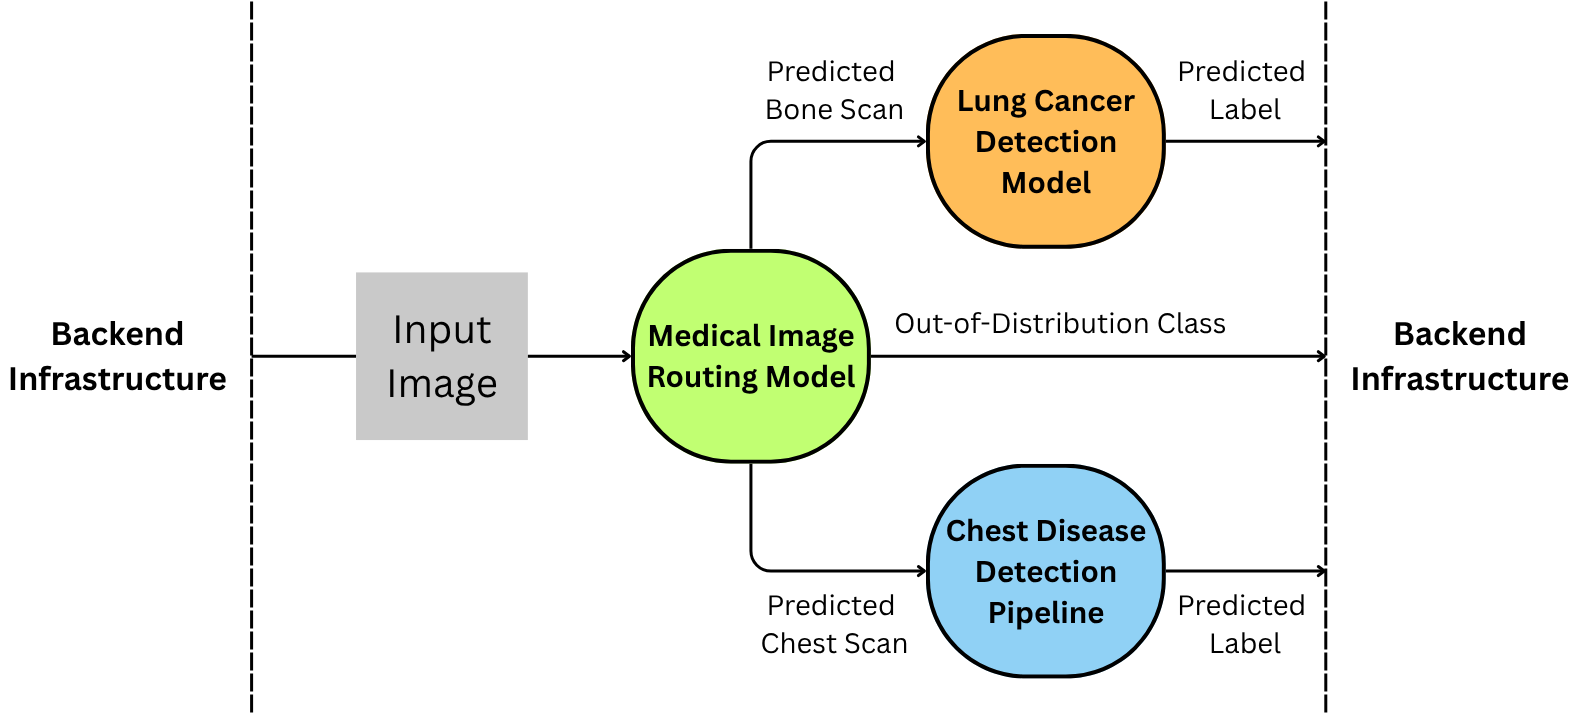
\includegraphics[width=\linewidth]{assets/full_project_arch.png}
	\caption{High-level architecture of the proposed framework. The system consists of a modality routing model, specialized disease classifiers, Explainable AI modules, and a Federated Learning infrastructure connecting multiple healthcare institutions.}
	\label{fig:full_overall_architecture}
\end{figure}

\subsection{Architectural Design Philosophy}

The proposed framework was developed according to several architectural principles that were established at the beginning of the system design process. These principles were intended to ensure that the resulting framework would not only achieve strong predictive performance but would also remain practical for real-world deployment in healthcare environments.

One of the most important design considerations was modality awareness. Medical images generated by different imaging technologies exhibit fundamentally different visual characteristics and diagnostic properties. Chest radiographs provide projection-based representations of thoracic structures, whereas CT scans generate detailed cross-sectional views that reveal significantly more anatomical information. These differences influence the types of features that neural networks must learn in order to perform accurate diagnosis. A single generalized model trained across multiple modalities may struggle to simultaneously learn optimal representations for all imaging types. Consequently, the proposed architecture explicitly separates modality identification from disease diagnosis. This design allows each diagnostic model to focus exclusively on data originating from the modality for which it was designed.

Another fundamental design principle was task specialization. The diseases targeted by this work differ substantially in terms of pathological manifestations, imaging characteristics, and diagnostic requirements. COVID-19, Tuberculosis, and Pneumonia are primarily identified using chest radiographs, whereas lung cancer diagnosis often relies on the higher anatomical resolution available in CT imaging. Rather than attempting to train a single network to recognize all diseases across all modalities, the proposed framework distributes these tasks among specialized models. This decomposition reduces task complexity and allows each model to learn more discriminative feature representations relevant to its specific diagnostic objective.

Reliability and patient safety also played a significant role in the architectural design. Medical AI systems must operate in environments where unexpected inputs are inevitable. Hospital information systems frequently contain diverse imaging studies, and a deployed diagnostic model may encounter unsupported image types, corrupted files, incomplete scans, or non-medical images. If such inputs are processed without validation, the resulting predictions may be unreliable and potentially dangerous. To address this issue, the proposed framework incorporates an explicit out-of-distribution detection mechanism within the routing stage. This component enables the system to identify unsupported inputs before they reach the diagnostic models.

Transparency represents another critical requirement for healthcare AI systems. Clinical practitioners often require evidence supporting automated predictions before integrating them into their decision-making processes. While deep neural networks have demonstrated remarkable predictive capabilities, they are frequently criticized for their lack of interpretability. The proposed architecture therefore integrates explainability mechanisms directly into the diagnostic workflow. These mechanisms provide visual explanations that highlight image regions contributing to the final prediction, thereby allowing clinicians to better understand and validate the reasoning process of the model.

Finally, the architecture was designed with scalability and long-term deployment in mind. Healthcare institutions are often unable to share patient data due to privacy regulations, legal restrictions, and ethical concerns. Consequently, the framework incorporates Federated Learning capabilities that enable multiple institutions to collaboratively improve model performance without exchanging raw patient information. This design promotes the creation of a continuously improving diagnostic ecosystem while preserving patient confidentiality.

\subsection{System Workflow}

The complete workflow of the proposed framework begins when a medical image is submitted to the system. Following acquisition, the image undergoes preprocessing operations intended to standardize the input format and improve compatibility with the downstream neural networks. These operations may include resizing, normalization, intensity standardization, and other transformations required by the underlying deep learning models.

Once preprocessing is completed, the image is forwarded to the first level of the architecture, namely the modality routing model. The purpose of this stage is to determine the nature of the input image and identify the appropriate diagnostic pathway. The routing decision governs all subsequent processing stages and therefore serves as a critical component of the framework.

After the routing decision is generated, the image is directed toward a specialized diagnostic model. Images identified as chest radiographs are analyzed by the chest disease classifier, while CT scans are analyzed by the lung cancer detection model. Images identified as out-of-distribution are excluded from automated diagnosis and may instead be flagged for manual review by healthcare personnel.

Following disease prediction, explainability modules generate visual interpretations of the model output. These interpretations provide insight into the image regions that most strongly influenced the prediction process. Finally, the prediction and associated explanation are presented to the clinician. During model training, Federated Learning mechanisms facilitate collaborative model improvement across multiple participating institutions.

Figure~\ref{fig:classification_tree} illustrates the classification pathway implemented by the proposed framework.

\begin{figure}[H]
	\centering
	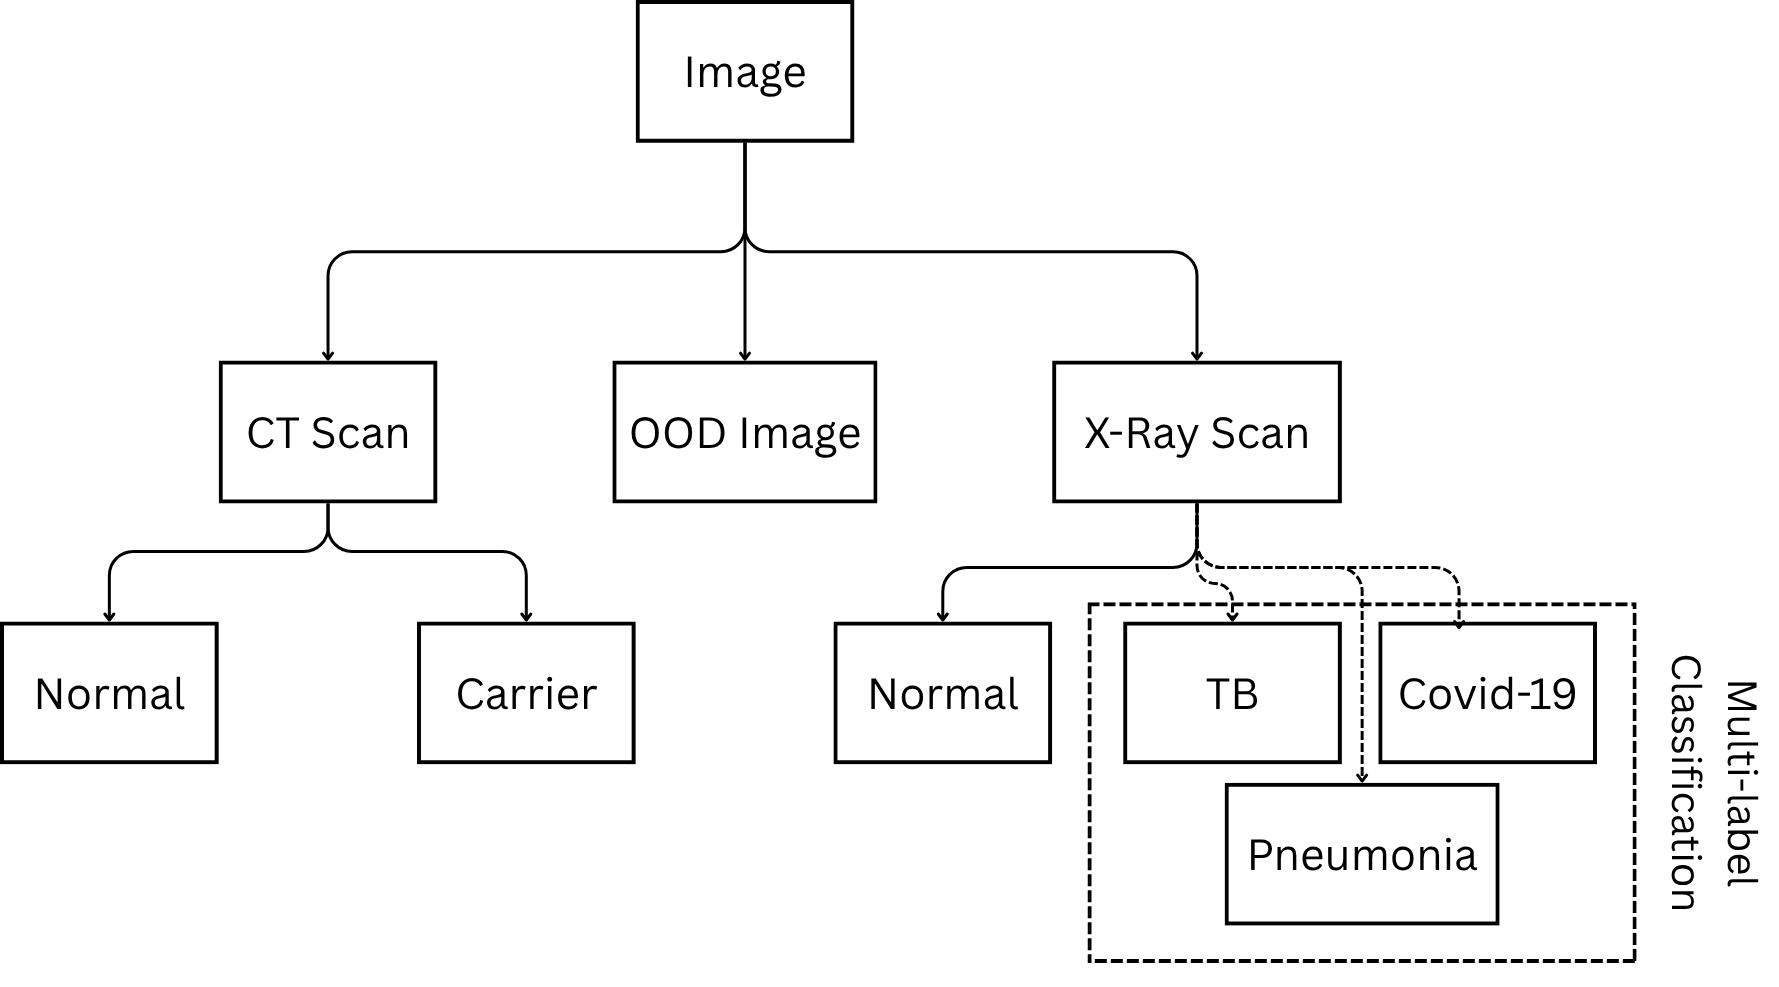
\includegraphics[width=0.8\linewidth]{assets/classification_tree.png}
	\caption{Classification tree of the proposed two-level framework. The routing model first determines the image modality before directing the image toward the appropriate disease-specific classifier.}
	\label{fig:classification_tree}
\end{figure}

\subsection{Level One: Modality Routing and Out-of-Distribution Detection}

The first level of the proposed architecture functions as an intelligent routing mechanism responsible for identifying the modality of the incoming image. Although this component performs a relatively simple classification task compared to disease diagnosis, its importance should not be underestimated. Every subsequent prediction generated by the framework depends directly on the correctness of the routing decision.

Formally, let $I$ denote an input image. The routing model $R(\cdot)$ maps the image into one of three categories:

\begin{equation}
	R(I) \in \{\text{X-ray}, \text{CT}, \text{OOD}\}
\end{equation}

where OOD represents an out-of-distribution image.

The motivation for introducing a dedicated routing stage arises from the substantial differences between X-ray and CT imaging modalities. Chest radiographs represent two-dimensional projection images that summarize anatomical information along a viewing direction. In contrast, CT scans provide detailed cross-sectional information that enables the visualization of internal structures with considerably greater precision. These differences imply that the features required for effective diagnosis are modality-dependent. Routing images to specialized models therefore allows the framework to exploit modality-specific representations rather than relying on a generalized feature extraction strategy.

From a computational perspective, routing also improves efficiency. Without this stage, every image would need to be processed by every available diagnostic model, resulting in increased computational cost and unnecessary inference overhead. By ensuring that each image is evaluated only by the most relevant classifier, the routing model reduces resource consumption and improves scalability.

An equally important function of the routing stage is out-of-distribution detection. In practical deployment scenarios, healthcare systems may receive images that differ significantly from those used during training. Examples include magnetic resonance imaging studies, ultrasound images, pathology slides, non-medical photographs, or improperly formatted files. Diagnostic models are generally incapable of producing reliable predictions for such inputs because they fall outside the distribution of the training data.

To mitigate this problem, the routing model incorporates a dedicated OOD category. Images assigned to this category are prevented from entering the diagnostic pipeline. This safeguard reduces the likelihood of erroneous predictions and contributes to the overall reliability of the framework. From a clinical perspective, this mechanism functions as a preliminary quality-control layer that ensures only supported image types proceed to automated analysis.

\subsection{Level Two: Chest Disease Detection Model}

Images identified as chest radiographs are forwarded to the chest disease classification model. This model is responsible for detecting three clinically significant respiratory diseases: COVID-19, Tuberculosis, and Pneumonia.

The selection of these diseases was motivated by both clinical relevance and public health importance. COVID-19 remains one of the most extensively studied respiratory illnesses in recent years and has highlighted the importance of rapid imaging-based screening techniques. Tuberculosis continues to represent a major global health challenge, particularly in developing countries where early detection plays a crucial role in disease management and transmission control. Pneumonia remains one of the most common respiratory infections worldwide and is associated with substantial morbidity and mortality across multiple age groups.

A key characteristic of the proposed chest disease model is its formulation as a multi-label classification problem rather than a conventional multi-class classification problem. This distinction is essential because the targeted diseases are not mutually exclusive. In clinical practice, a patient may simultaneously exhibit radiological findings associated with multiple respiratory conditions. For example, viral infections may be accompanied by secondary bacterial pneumonia, and complex pathological interactions may lead to overlapping imaging manifestations.

Traditional multi-class classification assumes that each sample belongs to exactly one category. Such an assumption would force the model to select a single disease label even when multiple diseases are present. This formulation would therefore fail to accurately represent many real-world clinical scenarios.

To address this limitation, the proposed architecture employs independent disease predictions. Let

\begin{equation}
	\mathbf{y} =
	[y_{\text{COVID}}, y_{\text{TB}}, y_{\text{Pneumonia}}]
\end{equation}

denote the output vector generated by the classifier. Each element corresponds to the estimated probability that a specific disease is present within the image.

Unlike a softmax-based multi-class architecture, the output layer uses independent sigmoid activations. This allows the model to assign high probabilities to multiple diseases simultaneously whenever appropriate. The final prediction for each disease is obtained by applying a predefined threshold:

\begin{equation}
	\hat{y}_i=
	\begin{cases}
		1 & y_i \geq \tau \\
		0 & y_i < \tau
	\end{cases}
\end{equation}

where $\tau$ denotes the classification threshold.

This formulation better reflects the realities of clinical diagnosis and provides greater flexibility when interpreting model outputs. Instead of receiving a single categorical prediction, clinicians are presented with independent disease probabilities that can be incorporated into broader diagnostic assessments.

\subsection{Level Two: Lung Cancer Detection Model}

Images classified as CT scans are forwarded to the lung cancer detection model. The decision to utilize CT imaging for lung cancer analysis is motivated by the superior anatomical detail provided by computed tomography compared to conventional radiography.

Lung cancer frequently manifests through subtle structural abnormalities such as pulmonary nodules, irregular masses, and localized tissue changes that may not be visible in chest radiographs. The high spatial resolution of CT imaging enables these features to be observed with significantly greater clarity, making CT the preferred modality for many lung cancer screening and diagnostic procedures.

The objective of the lung cancer model is to determine whether cancer-related findings are present within the input scan. The classifier can be represented mathematically as

\begin{equation}
	P_{\text{Cancer}} = C(I)
\end{equation}

where $C(\cdot)$ denotes the lung cancer detection network and $P_{\text{Cancer}}$ represents the estimated probability of malignancy.

By focusing exclusively on CT-derived information, the model can dedicate its representational capacity to learning highly discriminative cancer-related features. This specialization improves the model's ability to identify subtle pathological patterns that may be difficult to detect using a generalized classifier.

\subsection{Explainable Artificial Intelligence Integration}

The increasing adoption of artificial intelligence within healthcare has generated significant interest in model interpretability. Although deep learning systems are capable of achieving remarkable predictive performance, their internal decision-making processes often remain difficult to understand. This lack of transparency can hinder clinical adoption, particularly when predictions influence critical healthcare decisions.

To address this challenge, Explainable Artificial Intelligence techniques are integrated directly into the proposed architecture. Rather than treating explainability as an optional post-processing step, it is considered a fundamental component of the diagnostic workflow.

Following prediction generation, the explainability module produces visual explanations illustrating the regions of the image that most strongly influenced the model's decision. These visualizations may take the form of saliency maps, activation maps, attention maps, or gradient-based explanations depending on the selected implementation.

The integration of explainability serves several purposes. First, it increases clinician confidence by providing visual evidence supporting the model's prediction. Second, it facilitates model validation by enabling researchers to verify that the network is focusing on medically meaningful regions rather than irrelevant artifacts. Third, it assists in identifying potential biases or failure modes that may otherwise remain hidden within the network. Ultimately, explainability strengthens the collaborative relationship between clinicians and AI systems by transforming predictions into interpretable decision-support information.

\subsection{Federated Learning Infrastructure}

A distinguishing feature of the proposed framework is its support for Federated Learning. This capability was incorporated to address one of the most significant challenges facing medical artificial intelligence: limited access to large and diverse datasets.

Traditional deep learning systems typically rely on centralized training approaches in which data from multiple institutions are collected and stored in a single repository. While effective from a machine learning perspective, this strategy introduces substantial privacy, security, and regulatory concerns. Healthcare organizations are often prohibited from sharing patient data due to legal and ethical restrictions.

Federated Learning offers an alternative paradigm in which training occurs locally at each institution. Rather than transmitting patient data, participating hospitals train local models using their own datasets and share only model parameters or parameter updates. These updates are subsequently aggregated to produce a global model.

Let $w_i$ denote the model parameters learned by institution $i$, and let $n_i$ denote the number of training samples available at that institution. Using the Federated Averaging algorithm, the global model is computed as

\begin{equation}
	w_{\text{global}}
	=
	\sum_{i=1}^{K}
	\frac{n_i}{\sum_{j=1}^{K}n_j}
	w_i
\end{equation}

where $K$ represents the total number of participating institutions.

Beyond privacy preservation, Federated Learning provides several additional benefits. Because participating institutions often serve different patient populations, the resulting datasets contain greater demographic, geographic, and clinical diversity. Training across such heterogeneous data sources can improve model generalization and reduce susceptibility to institution-specific biases. Furthermore, the collaborative nature of Federated Learning enables continuous improvement of the framework as new institutions join the network and contribute additional knowledge.


\section{Transfer-Learning Models Used}
This section presents the transfer learning models employed in the proposed system and discusses the rationale behind their selection. Transfer learning is adopted to leverage pre-trained deep neural networks that have been trained on large-scale datasets, enabling effective feature extraction and improved generalization in medical imaging tasks with limited labeled data. The section provides an overview of the selected architectures and highlights their suitability for different components of the proposed diagnostic pipeline.

\subsection{ResNet50 Model} \label{subsec:resnet50-arch}
Residual Networks (ResNets) were introduced to address the degradation problem observed in deep convolutional neural networks, where increasing network depth leads to saturation or decline in training accuracy. This issue emerges due to optimization difficulties such as vanishing gradients. ResNet addresses this limitation through the concept of residual learning, which allows the training of substantially deeper networks by enabling more effective gradient propagation.

The key idea of residual learning is to reformulate the learning objective of a neural network block. Instead of directly learning a desired underlying mapping \( H(x) \), a residual block learns a residual function \( F(x) \) such that:
\[
H(x) = F(x) + x
\]
where \( x \) represents the input to the residual block and \( F(x) \) represents the output of the stacked convolutional layers within the block. The identity shortcut connection that performs the addition allows gradients to flow directly through the network during backpropagation, thereby minimizing vanishing gradient effects and improving training stability.

\begin{figure}[h]
	\centering
	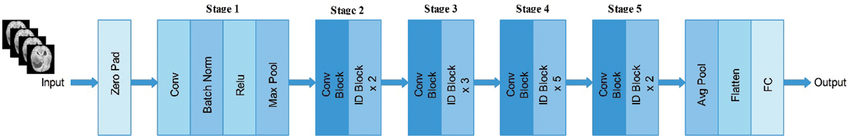
\includegraphics[width=\linewidth]{assets/resnet50.png}
	\caption{Architecture of the ResNet50 illustrating the successive stages of the model.}
	\label{fig:resnet50-arch}
\end{figure}

As illustrated in Figure~\ref{fig:resnet50-arch}, the ResNet50 architecture begins with an initial convolutional layer preceded by zero padding, followed by batch normalization, a ReLU activation function, and a max pooling operation. This initial stage is responsible for extracting low-level visual features from the input image. The network then proceeds through five sequential stages composed of convolutional blocks and identity blocks, each incorporating residual connections that bypass multiple convolutional layers.

ResNet50 employs a bottleneck design within its residual blocks, consisting of a sequence of \(1 \times 1\), \(3 \times 3\), and \(1 \times 1\) convolutional layers. The \(1 \times 1\) convolutions are used to reduce and subsequently restore feature dimensionality, thereby decreasing computational complexity while preserving representational power. This design enables ResNet50 to achieve substantial depth without incurring prohibitive computational costs.

Compared to shallower variants such as ResNet18 and ResNet34, ResNet50 offers increased representational capacity and improved ability to capture complex and abstract visual patterns. While deeper variants such as ResNet101 and ResNet152 further extend network depth, they introduce higher computational overhead and an increased risk of overfitting, particularly in medical imaging applications where annotated data is often limited. Consequently, ResNet50 represents a balanced trade-off between depth, efficiency, and performance within the ResNet family.

As shown in Figure~\ref{fig:resnet50-arch}, the final stages of ResNet50 consist of a global average pooling layer, followed by feature flattening and a fully connected layer. In transfer learning scenarios, this classification head can be replaced or fine-tuned to adapt the network to domain-specific medical tasks.

In the context of medical image analysis, ResNet50 is well-suited for extracting both low-level structural features and high-level semantic representations relevant to pathological patterns. The residual connections promote feature reuse and robust optimization, which is particularly important for detecting subtle abnormalities in medical images such as fractures or thoracic diseases. These characteristics make ResNet50 a reliable and widely adopted backbone for medical image classification tasks.

\subsection{DenseNet121 Model}
\label{subsec:densenet121}

DenseNet121 is a deep convolutional neural network architecture belonging to the family of Densely Connected Convolutional Networks (DenseNets), which were introduced by Huang \textit{et al.} in 2017 to address several limitations associated with traditional deep neural networks. DenseNet architectures were designed to improve feature propagation, encourage feature reuse, alleviate the vanishing gradient problem, and reduce the number of trainable parameters while maintaining high classification performance. Since its introduction, DenseNet121 has become one of the most widely adopted architectures in medical image analysis due to its ability to learn rich hierarchical representations from relatively limited datasets.

The fundamental idea behind DenseNet differs significantly from that of conventional convolutional neural networks. In traditional architectures, each layer receives information only from the immediately preceding layer and passes its output solely to the next layer. Although this sequential information flow is effective, it may lead to difficulties in gradient propagation as network depth increases. Furthermore, many learned feature maps become redundant because similar patterns are repeatedly relearned at different layers throughout the network.

To address these limitations, DenseNet introduces direct connections between layers. Instead of receiving input from only the previous layer, each layer receives the feature maps generated by all preceding layers within the same dense block. Consequently, information can flow directly from earlier layers to later layers without repeatedly passing through intermediate transformations. This dense connectivity pattern enables more efficient feature reuse and facilitates the training of very deep networks.

Figure~\ref{fig:densenet121_architecture} illustrates the overall architecture of DenseNet121.

\begin{figure}[H]
	\centering
	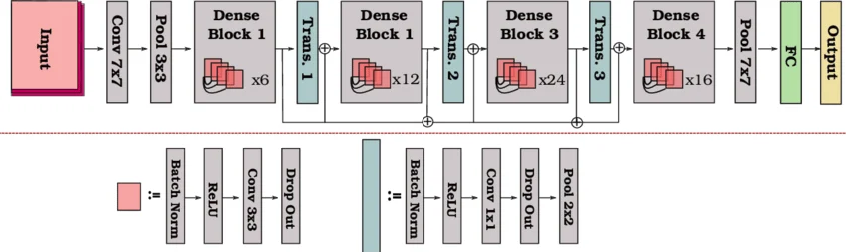
\includegraphics[width=\linewidth]{assets/DenseNet121.png}
	\caption{Overall architecture of DenseNet121 showing the arrangement of dense blocks, transition layers, and the final classification stage.}
	\label{fig:densenet121_architecture}
\end{figure}

\subsubsection{Motivation Behind Dense Connectivity}

As neural networks become deeper, the flow of information and gradients through the network becomes increasingly difficult. One of the most common challenges encountered in deep architectures is the vanishing gradient problem, where gradients become progressively smaller as they are propagated backward through many layers. When gradients become extremely small, early layers receive little useful learning signal, slowing convergence and potentially reducing overall performance.

Residual Networks (ResNets) partially addressed this issue through skip connections that allow gradients to bypass certain transformations. DenseNet extends this concept further by establishing direct connections between every pair of layers within a dense block. Instead of merely adding outputs from previous layers, DenseNet concatenates them. This strategy preserves information from all preceding layers and makes it directly accessible to subsequent layers.

The dense connectivity mechanism provides several important benefits. First, it improves gradient flow during training, allowing deeper networks to be optimized more effectively. Second, it encourages feature reuse, reducing redundancy among learned representations. Third, it improves parameter efficiency because layers can leverage previously learned features rather than learning entirely new representations from scratch.

\subsubsection{Dense Connectivity Mechanism}

The defining characteristic of DenseNet is the dense connection pattern between layers. Let $x_0$ represent the input to a dense block and let $x_l$ denote the output of the $l^{th}$ layer. Unlike traditional convolutional networks, where the output of layer $l$ depends only on the output of layer $l-1$, DenseNet computes each layer using the outputs of all preceding layers:

\begin{equation}
	x_l = H_l([x_0, x_1, x_2, ..., x_{l-1}])
\end{equation}

where:

\begin{itemize}
	\item $H_l(\cdot)$ denotes a composite transformation.
	\item $[\cdot]$ represents the concatenation operation.
	\item $x_0, x_1, ..., x_{l-1}$ are the feature maps generated by previous layers.
\end{itemize}

The concatenation operation differs fundamentally from the addition operation used in residual networks. Instead of merging features by summation, DenseNet preserves all previous feature maps and passes them directly to subsequent layers. As a result, each layer has access to both low-level and high-level information simultaneously.

This dense feature propagation mechanism allows later layers to exploit a richer collection of learned representations, improving feature diversity and reducing information loss.

\subsubsection{Dense Blocks}

The primary computational components of DenseNet121 are the dense blocks. A dense block consists of multiple densely connected layers arranged according to the connectivity pattern described previously.

Within each dense block, every layer receives as input the concatenated outputs of all preceding layers. Consequently, the number of feature maps grows progressively as additional layers are added. This growth is controlled through a parameter known as the \textit{growth rate}.

The growth rate, typically denoted by $k$, determines the number of new feature maps generated by each layer. If the input to a dense block contains $F_0$ feature maps and the block contains $L$ layers, the total number of feature maps at the end of the block can be expressed as:

\begin{equation}
	F = F_0 + kL
\end{equation}

where:

\begin{itemize}
	\item $F_0$ is the number of initial feature maps.
	\item $k$ is the growth rate.
	\item $L$ is the number of layers within the block.
\end{itemize}

For DenseNet121, the growth rate is typically set to 32. This means that each layer contributes 32 new feature maps while simultaneously utilizing all previously generated feature maps.

The use of a relatively small growth rate contributes to the parameter efficiency of DenseNet architectures, allowing them to achieve competitive performance with fewer parameters than many alternative architectures.

\subsubsection{Composite Function within Dense Layers}

Each layer within a dense block consists of a sequence of operations designed to transform incoming feature maps into more informative representations.

The composite transformation $H_l(\cdot)$ generally consists of:

\begin{enumerate}
	\item Batch Normalization (BN)
	\item Rectified Linear Unit (ReLU)
	\item Convolution
\end{enumerate}

This sequence is commonly referred to as the BN-ReLU-Conv pattern.

Batch normalization stabilizes the learning process by normalizing intermediate activations. This reduces internal covariate shift and allows higher learning rates to be used during training.

The ReLU activation function introduces non-linearity into the network and is defined as:

\begin{equation}
	f(x) = \max(0,x)
\end{equation}

Following activation, convolutional filters extract spatial patterns from the input feature maps. Through repeated application of these operations, the network gradually learns increasingly abstract representations of the input image.

\subsubsection{Bottleneck Layers}

As the number of feature maps grows within dense blocks, computational complexity can increase significantly. To reduce this cost, DenseNet121 employs bottleneck layers.

A bottleneck layer consists of a $1 \times 1$ convolution applied before the standard $3 \times 3$ convolution. The purpose of this operation is to reduce the number of feature channels while preserving important information.

The bottleneck structure can be summarized as:

\begin{equation}
	BN \rightarrow ReLU \rightarrow Conv(1\times1)
	\rightarrow BN \rightarrow ReLU \rightarrow Conv(3\times3)
\end{equation}

The use of bottleneck layers substantially reduces computational requirements while maintaining representational capacity.

\subsubsection{Transition Layers}

Because feature map dimensions increase continuously within dense blocks, DenseNet introduces transition layers between consecutive blocks to control network complexity.

A transition layer performs two primary functions. First, it reduces the number of feature maps through a $1 \times 1$ convolution. Second, it decreases spatial resolution using average pooling.

The transition layer architecture typically follows:

\begin{equation}
	BN \rightarrow ReLU \rightarrow Conv(1\times1)
	\rightarrow AvgPool(2\times2)
\end{equation}

These operations prevent excessive growth in memory consumption while preserving the most informative features.

Transition layers also contribute to hierarchical feature extraction by gradually reducing spatial dimensions as network depth increases.

\subsubsection{Architecture of DenseNet121}

DenseNet121 consists of four dense blocks separated by three transition layers. The architecture begins with an initial convolution layer and concludes with global average pooling followed by a fully connected classification layer.

The distribution of layers across dense blocks is as follows:

\begin{table}[H]
	\centering
	\caption{Layer distribution within DenseNet121.}
	\begin{tabular}{|c|c|}
		\hline
		Component & Number of Layers \\
		\hline
		Dense Block 1 & 6 \\
		Dense Block 2 & 12 \\
		Dense Block 3 & 24 \\
		Dense Block 4 & 16 \\
		\hline
		Total Dense Layers & 58 \\
		\hline
	\end{tabular}
	\label{tab:densenet121_blocks}
\end{table}

When all convolutional, pooling, and classification layers are included, the network contains 121 trainable layers, which gives the architecture its name.

The input image first passes through an initial $7\times7$ convolution layer followed by max pooling. Feature extraction then proceeds through the sequence of dense blocks and transition layers. Finally, global average pooling aggregates spatial information into a compact feature vector, which is passed to the final classification layer.

\subsubsection{Advantages of DenseNet121 for Medical Image Analysis}

DenseNet121 possesses several characteristics that make it particularly suitable for medical image classification tasks.

The dense connectivity pattern encourages extensive feature reuse, allowing the network to learn robust representations even when training datasets are relatively small. This characteristic is especially important in medical imaging, where acquiring large annotated datasets is often challenging.

The improved gradient flow resulting from dense connections facilitates stable optimization and reduces the risk of vanishing gradients. Consequently, deeper representations can be learned without the training difficulties commonly associated with very deep neural networks.

DenseNet121 is also highly parameter-efficient compared to many competing architectures. Despite its depth, the network requires fewer trainable parameters than several traditional convolutional architectures because previously learned features are reused rather than repeatedly regenerated.

Furthermore, the architecture has demonstrated strong performance across a wide range of medical imaging applications, including chest disease classification, pneumonia detection, COVID-19 diagnosis, tuberculosis screening, diabetic retinopathy analysis, and cancer detection. Its proven effectiveness in healthcare applications has made DenseNet121 a popular backbone network for medical image analysis research.

\subsubsection{DenseNet121 in the Proposed Framework}

In the context of this work, DenseNet121 was selected as the backbone architecture for the first-level routing model due to its strong balance between classification performance, computational efficiency, and feature extraction capability. The dense connectivity structure enables the model to capture both low-level radiological patterns and high-level pathological characteristics that are essential for accurate disease recognition.

Additionally, the feature reuse mechanism of DenseNet121 is particularly advantageous for medical datasets, where image variability can be substantial and labeled samples may be limited. By leveraging information from all preceding layers, the network can construct rich hierarchical representations that support robust classification performance.

Overall, DenseNet121 provides a powerful and efficient deep learning architecture that aligns well with the requirements of medical image analysis systems. Its dense connectivity, parameter efficiency, strong gradient propagation, and proven effectiveness in healthcare applications make it an appropriate choice for the disease classification tasks addressed in this project.

\subsection{YOLOv8 Model} \label{subsec:yolo}

\begin{figure}[H]
	\centering
	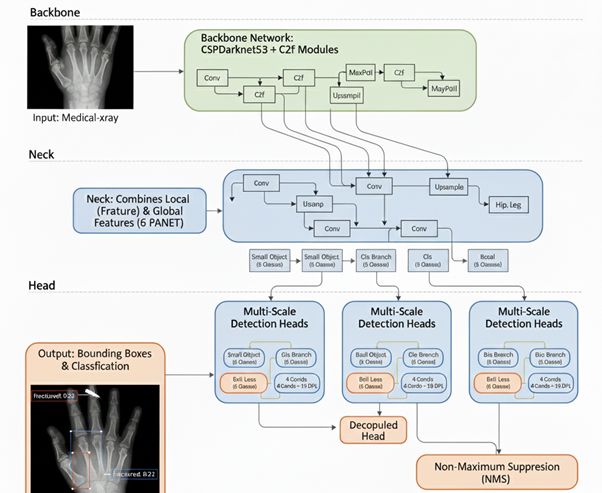
\includegraphics[width=\linewidth]{assets/yolo-arch.png}
	\caption{General architecture of YOLOv8 illustrating the backbone, neck, and detection head components.}
	\label{fig:yolo-arch}
\end{figure}

Object detection has become one of the most important computer vision tasks in modern medical image analysis due to its ability to simultaneously identify and localize pathological findings within an image. Unlike conventional image classification models that only determine whether a disease is present, object detection models additionally provide spatial information regarding the location of abnormalities. This capability is particularly valuable in lung cancer diagnosis, where clinicians must not only determine the presence of a suspicious lesion but also identify its precise location within the lungs.

In the proposed framework, lung cancer detection is formulated as an object detection problem rather than a traditional image classification task. Instead of predicting a single label for an entire CT scan, the model identifies suspicious cancerous regions and generates bounding boxes surrounding them. To accomplish this task, the proposed system employs YOLOv8 (You Only Look Once Version 8), one of the most recent and advanced members of the YOLO family of object detection architectures.

YOLOv8 is a single-stage object detector, meaning that object localization and classification are performed within a single forward pass through the network. This design significantly reduces computational complexity compared to two-stage detectors such as Faster R-CNN, which first generate candidate regions and subsequently classify them. By combining both operations into a unified architecture, YOLOv8 achieves high detection accuracy while maintaining efficient inference speeds. These characteristics make it particularly suitable for deployment within real-time clinical decision support systems where rapid analysis of CT scans is desirable.

The complete processing pipeline employed by the proposed lung cancer detection model is illustrated in Figure~\ref{fig:yolo_pipeline}.

\begin{figure}[H]
	\centering
	
	\resizebox{\linewidth}{!}{
		\begin{tabular}{c c c c c c c c c c c}
			\fbox{
				\begin{tabular}{c}
					Chest CT\\
					Input
				\end{tabular}
			}
			&
			$\rightarrow$
			&
			\fbox{
				\begin{tabular}{c}
					Image\\
					Preprocessing
				\end{tabular}
			}
			&
			$\rightarrow$
			&
			\fbox{
				\begin{tabular}{c}
					YOLOv8\\
					Backbone
				\end{tabular}
			}
			&
			$\rightarrow$
			&
			\fbox{
				\begin{tabular}{c}
					PANet\\
					Neck
				\end{tabular}
			}
			&
			$\rightarrow$
			&
			\fbox{
				\begin{tabular}{c}
					Detection\\
					Head
				\end{tabular}
			}
			&
			$\rightarrow$
			&
			\fbox{
				\begin{tabular}{c}
					Lung Cancer\\
					Detection
				\end{tabular}
			}
		\end{tabular}
	}
	
	\caption{End-to-end processing pipeline of the proposed YOLOv8 lung cancer detection model.}
	\label{fig:yolo_pipeline}
\end{figure}

As illustrated in Figure~\ref{fig:yolo-arch}, YOLOv8 consists of three primary components: the backbone, the neck, and the detection head. Each component contributes a specific functionality to the overall detection process.

\subsubsection{Backbone Network}

The backbone serves as the feature extraction component of YOLOv8. Its primary objective is to transform raw CT scan images into hierarchical feature representations that can be used for lesion detection. YOLOv8 employs the C2f (Cross-Stage Partial Bottleneck with Two Convolutions) architecture, which is an evolution of the CSP (Cross Stage Partial) designs used in previous YOLO versions.

The backbone progressively applies convolutional operations to the input image, generating increasingly abstract feature maps. Early layers learn low-level visual characteristics such as edges, gradients, and texture variations, while deeper layers capture more complex semantic information associated with pulmonary nodules, masses, and abnormal tissue structures.

One of the key advantages of the C2f architecture is its ability to improve gradient propagation while reducing computational overhead. By reusing features across multiple layers, the network can learn richer representations without requiring excessive numbers of parameters. This characteristic is particularly beneficial in medical imaging applications where datasets are often smaller than those available in general computer vision tasks.

For lung cancer detection, the backbone learns to distinguish subtle visual differences between healthy lung tissue and suspicious lesions. These differences may include variations in density, texture, shape, and intensity patterns that are characteristic of malignant abnormalities.

\subsubsection{Neck Network}

The neck component is responsible for feature aggregation and multi-scale feature fusion. In YOLOv8, this functionality is implemented using a Path Aggregation Network (PANet).

Feature extraction layers at different depths of the backbone capture information at different scales. Shallow layers retain detailed spatial information, while deeper layers capture more abstract semantic features. Because lung cancer lesions can vary significantly in size, relying on a single feature scale would limit detection performance.

Small pulmonary nodules may occupy only a tiny portion of the CT image, whereas larger tumors may extend across substantial regions of the lung. The PANet structure addresses this challenge by combining feature maps generated at multiple scales. Through repeated top-down and bottom-up information flow, PANet enables the model to simultaneously utilize local texture details and broader anatomical context.

Consequently, the neck allows YOLOv8 to detect both small and large lesions while maintaining accurate localization performance across a wide range of tumor sizes.

\subsubsection{Detection Head}

The final component of YOLOv8 is the detection head. This module is responsible for generating the actual predictions produced by the network.

Unlike earlier object detectors that relied on predefined anchor boxes, YOLOv8 employs an anchor-free detection strategy. Rather than predicting offsets relative to predetermined anchors, the model directly predicts object centers and bounding box coordinates.

The detection head performs two independent tasks:

\begin{itemize}
	\item Classification of detected regions.
	\item Localization of detected lesions.
\end{itemize}

This decoupled architecture allows each task to be optimized independently, improving overall detection performance. For each detected region, the model predicts:

\begin{itemize}
	\item Bounding box coordinates.
	\item Object confidence score.
	\item Cancer detection probability.
\end{itemize}

The resulting predictions are then forwarded to the post-processing stage for refinement.

\subsubsection{Multi-Scale Detection}

A major challenge in lung cancer detection is the substantial variability in lesion size. Early-stage tumors may appear as extremely small nodules, whereas advanced-stage tumors can occupy large portions of the lung field.

YOLOv8 addresses this challenge through multi-scale detection. Detection heads operate on feature maps of different resolutions, enabling the model to identify abnormalities across multiple spatial scales.

This capability is particularly important in CT-based diagnosis because the early detection of small nodules is often critical for improving patient outcomes. Multi-scale processing allows the model to preserve fine-grained details while simultaneously leveraging high-level semantic information extracted from deeper network layers.

The full process of multi-scale feature extraction is shown in Figure~\ref{fig:yolo_multiscale}

\begin{figure}[H]
	\centering
	
	\begin{tabular}{ccc}
		
		\fbox{
			\begin{minipage}{0.25\textwidth}
				\centering
				High-Resolution Features\\
				(Small Nodules)
			\end{minipage}
		}
		
		&
		
		\fbox{
			\begin{minipage}{0.25\textwidth}
				\centering
				Medium-Resolution Features\\
				(Intermediate Lesions)
			\end{minipage}
		}
		
		&
		
		\fbox{
			\begin{minipage}{0.25\textwidth}
				\centering
				Low-Resolution Features\\
				(Large Tumors)
			\end{minipage}
		}
		
	\end{tabular}
	
	\vspace{0.5cm}
	
	$\downarrow$
	
	\vspace{0.3cm}
	
	\fbox{
		\begin{minipage}{0.4\textwidth}
			\centering
			Unified Multi-Scale Detection Output
		\end{minipage}
	}
	
	\caption{Multi-scale feature extraction employed by YOLOv8 for detecting lung lesions of varying sizes.}
	\label{fig:yolo_multiscale}
\end{figure}

\subsubsection{Anchor-Free Detection Mechanism}

Traditional object detection models rely on predefined anchor boxes that attempt to approximate the expected shapes and sizes of target objects. Although effective in many applications, anchor-based methods introduce additional hyperparameters and often struggle with irregularly shaped objects.

Lung tumors exhibit substantial variability in morphology and rarely conform to standardized geometric patterns. Consequently, anchor-based approaches may fail to adequately represent their boundaries.

YOLOv8 addresses this limitation by adopting an anchor-free detection strategy. Instead of matching objects to predefined anchor templates, the model directly predicts object centers and corresponding bounding box coordinates.

This design offers several advantages:

\begin{itemize}
	\item Reduced hyperparameter complexity.
	\item Improved adaptability to irregular tumor shapes.
	\item Faster convergence during training.
	\item Enhanced localization performance.
\end{itemize}

These characteristics make anchor-free detection particularly suitable for medical imaging applications involving heterogeneous pathological structures.

\subsubsection{Bounding Box Regression and Localization}

Once suspicious regions have been identified, YOLOv8 must determine the exact boundaries of each lesion.

Bounding box regression is performed by predicting:

\begin{itemize}
	\item Horizontal position.
	\item Vertical position.
	\item Width.
	\item Height.
\end{itemize}

These predictions are continuously refined throughout training using specialized localization loss functions. The resulting bounding boxes provide interpretable visual evidence regarding the location of suspicious findings and can assist clinicians during diagnostic review.

\subsubsection{Non-Maximum Suppression}

Object detectors frequently generate multiple overlapping predictions for the same lesion. To eliminate redundant detections, YOLOv8 employs Non-Maximum Suppression (NMS).

The process is illustrated in Figure~\ref{fig:yolo_nms}.

\begin{figure}[H]
	\centering
	
	\resizebox{0.95\linewidth}{!}{
		\begin{tabular}{c c c c c c c}
			
			\fbox{
				\begin{tabular}{c}
					Overlapping\\
					Bounding Boxes
				\end{tabular}
			}
			
			&
			$\rightarrow$
			&
			
			\fbox{
				\begin{tabular}{c}
					IoU\\
					Calculation
				\end{tabular}
			}
			
			&
			$\rightarrow$
			&
			
			\fbox{
				\begin{tabular}{c}
					Non-Maximum\\
					Suppression
				\end{tabular}
			}
			
			&
			$\rightarrow$
			&
			
			\fbox{
				\begin{tabular}{c}
					Final Lung Cancer\\
					Detection
				\end{tabular}
			}
			
		\end{tabular}
	}
	
	\caption{Non-Maximum Suppression procedure used to remove duplicate detections and retain the highest-confidence prediction.}
	\label{fig:yolo_nms}
\end{figure}

The overlap between predicted and ground-truth boxes is measured using the Intersection over Union (IoU) metric:

\[
IoU =
\frac
{
	Area(B_p \cap B_g)
}
{
	Area(B_p \cup B_g)
}
\]

where \(B_p\) denotes the predicted bounding box and \(B_g\) denotes the ground-truth bounding box.

Predictions with excessive overlap are suppressed, ensuring that each lesion is represented by a single final detection.

\subsubsection{Training Objective and Loss Functions}

YOLOv8 optimizes a composite loss function composed of multiple components.

\paragraph{Classification Loss (Binary Cross-Entropy)}

Binary Cross-Entropy loss guides the model in distinguishing cancerous lesions from background regions. This loss encourages accurate classification while minimizing false positive detections.

\paragraph{Box Localization Loss (CIoU)}

Complete Intersection over Union (CIoU) loss evaluates localization quality by considering overlap area, center distance, and aspect ratio differences between predicted and ground-truth boxes.

This loss can be expressed conceptually as:

\[
L_{CIoU}
=
1 - IoU
+
\text{Distance Penalty}
+
\text{Aspect Ratio Penalty}
\]

where additional penalty terms improve localization precision.

\paragraph{Distribution Focal Loss (DFL)}

Distribution Focal Loss improves boundary estimation by modeling uncertainty in bounding box coordinates. This is particularly important in medical images where lesion boundaries may be ambiguous or partially obscured.

Together, these loss functions allow YOLOv8 to simultaneously optimize classification accuracy and localization quality.

\subsubsection{Suitability of YOLOv8 for Lung Cancer Detection}

Several characteristics make YOLOv8 particularly suitable for lung cancer detection.

First, its single-stage architecture provides rapid inference speeds while maintaining high detection accuracy. This allows the model to be integrated into real-time diagnostic support systems.

Second, multi-scale feature extraction enables the detection of lesions exhibiting substantial size variation, ranging from small pulmonary nodules to larger malignant masses.

Third, the anchor-free detection mechanism improves adaptability to irregular tumor morphologies commonly encountered in clinical practice.

Fourth, the generated bounding boxes provide intuitive visual explanations that can assist clinicians in understanding and verifying model predictions.

Finally, YOLOv8 benefits from transfer learning, allowing knowledge acquired from large-scale image datasets to be leveraged for medical imaging tasks. This capability is especially valuable when working with limited annotated medical datasets.

To evaluate the effectiveness of the proposed lung cancer detection model, Precision, Recall, and mAP50 are employed as the primary performance metrics. Precision quantifies the proportion of detected lesions that are truly cancerous, Recall measures the proportion of actual lesions successfully identified by the model, and mAP50 provides a comprehensive assessment of overall detection performance by evaluating both localization and classification accuracy at an Intersection over Union threshold of 0.50.

Collectively, these metrics provide a rigorous evaluation of the model's ability to accurately identify and localize lung cancer lesions within chest CT scans, ensuring that the resulting system can serve as a reliable component of the proposed intelligent diagnostic framework.

\subsection{The CheXFound Vision Foundation Model and ViT Architecture}
\label{subsec:chexfound_vit}

To address the limitations of centralized and domain-restricted architectures under severe data siloing, modern clinical pipelines are shifting toward Vision Foundation Models (VFMs). At the forefront of this shift is \textbf{CheXFound}, a self-supervised, vision-centric foundation model engineered explicitly for high-throughput, multi-class thoracic imaging diagnosis. CheXFound eliminates the historical constraint of training standalone networks for separate diagnostic indications by building generalized, highly robust chest representations. By utilizing a heavy Vision Transformer (ViT) architecture rather than a conventional convolutional backbone, CheXFound effectively captures long-range dependencies, contextual anatomical relationships, and fine-grained pathological variations across heterogeneous image streams.

\subsubsection{The Vision Transformer (ViT-Large) Backbone Architecture}

CheXFound is structurally built upon a modified \textbf{ViT-Large (ViT-L/16)} structural spine, optimizing representation capabilities at an expanded spatial resolution of $512\times512$ pixels. This configuration is mathematically designed to process image grids without losing subtle pathological signals, such as micro-nodular patterns or faint ground-glass borders, which often disappear when compressed into lower-resolution latent matrices. 

The structural flow of the forward pass within CheXFound's ViT-L/16 architecture proceeds as follows:

\begin{enumerate}
	\item \textbf{Patch Extraction and Flattening:} A continuous two-dimensional input thoracic image $\mathbf{X} \in \mathbb{R}^{H \times W \times C}$ (where $H=W=512$ and $C=1$ for radiographs or single-slice CTs) is systematically split into a grid of non-overlapping, uniform rectangular patches $\mathbf{X}_p \in \mathbb{R}^{N \times (P^2 \cdot C)}$. Here, $P = 16$ denotes the hardcoded spatial patch size, and $N$ represents the resulting total number of sequence patches, computed mathematically as:
	\begin{equation}
		N = \frac{H \cdot W}{P^2} = \frac{512 \times 512}{16 \times 16} = 1024 \text{ patches}
	\end{equation}
	
	\item \textbf{Linear Patch Embedding:} Each flattened structural patch token is projected into a lower-dimensional latent embedding space using a trainable linear mapping matrix $\mathbf{E} \in \mathbb{R}^{(P^2 \cdot C) \times D}$, where $D = 1024$ defines the dense hidden embedding dimension of the ViT-Large backbone.
	
	\item \textbf{CLS Token Prepended and Position Encodings:} A learnable classification token embedding $\mathbf{z}_0^0 = \mathbf{x}_{\text{class}} \in \mathbb{R}^D$ is prepended to the sequence of patch tokens. To preserve the two-dimensional spatial topography of the chest inside a one-dimensional sequence pipeline, standard learnable one-dimensional position encodings $\mathbf{E}_{\text{pos}} \in \mathbb{R}^{(N+1) \times D}$ are element-wise added to the patch embeddings, yielding the initial input tensor $\mathbf{z}_0$:
	\begin{equation}
		\mathbf{z}_0 = \left[ \mathbf{x}_{\text{class}}; \, \mathbf{X}_p^1\mathbf{E}; \, \mathbf{X}_p^2\mathbf{E}; \, \dots; \, \mathbf{X}_p^N\mathbf{E} \right] + \mathbf{E}_{\text{pos}}
	\end{equation}
	
	\item \textbf{Transformer Encoder Blocks:} The combined sequence $\mathbf{z}_0$ passes sequentially through $L = 24$ identical Transformer Encoder blocks. Each block features a Multi-Head Self-Attention (\text{MHSA}) mechanism with $h = 16$ distinct attention heads, interleaved with Multi-Layer Perceptron (\text{MLP}) blocks and scaled by Layer Normalization (\text{LN}) using residual skip-connections:
	\begin{align}
		\mathbf{z}_{\ell}' &= \text{MHSA}(\text{LN}(\mathbf{z}_{\ell-1})) + \mathbf{z}_{\ell-1}, \quad \ell = 1, \dots, 24 \\
		\mathbf{z}_{\ell} &= \text{MLP}(\text{LN}(\mathbf{z}_{\ell}')) + \mathbf{z}_{\ell}'
	\end{align}
\end{enumerate}

The standard ViT core configuration embedded inside CheXFound is mathematically mapped and detailed in Table~\ref{tab:vit_large_specs}.

\begin{table}[htbp]
	\centering
	\caption{Structural and mathematical parameter configurations of the CheXFound ViT-Large/16 backbone layout.}
	\label{tab:vit_large_specs}
	\small
	\begin{tabularx}{\textwidth}{lXX}
		\toprule
		\textbf{Architectural Hyperparameter} & \textbf{Formal Definition / Notation} & \textbf{Deterministic Global Value} \\
		\midrule
		\textbf{Input Resolution} & $H \times W \times C$ & $512 \times 512 \times 1$ Pixels \\
		\addlinespace
		\textbf{Patch Dimension} & $P \times P$ & $16 \times 16$ Pixels \\
		\addlinespace
		\textbf{Sequence Count} & $N = (H \cdot W)/P^2$ & $1024$ Active Patch Tokens \\
		\addlinespace
		\textbf{Hidden Layer Dimension} & $D$ & $1024$ Scaled Scaling Dimensions \\
		\addlinespace
		\textbf{Transformer Layers} & $L$ & $24$ Cascaded Encoder Blocks \\
		\addlinespace
		\textbf{Attention Heads} & $h$ & $16$ Independent Heads \\
		\addlinespace
		\textbf{MLP Expansion Ratio} & $\text{Ratio}_{\text{MLP}}$ & $4.0 \times D$ ($4096$ Hidden Units) \\
		\bottomrule
	\end{tabularx}
\end{table}

\subsubsection{Pretraining Paradigm and Self-Supervised Objective Functions}

CheXFound is pretrained on a curated, large-scale medical dataset comprising approximately 987,000 unique chest radiographs derived from 12 distinct open-source clinical databases (including MIMIC-CXR, CheXpert, PadChest, and BraX). To extract optimal task-agnostic representations without relying on manual labels, CheXFound utilizes the **DINOv2** self-supervised learning pipeline. This setup combines a student network (parameterized by weights $\theta_s$) and a teacher network (parameterized by weights $\theta_t$). The teacher's weights are updated continuously via an Exponential Moving Average (EMA) of the student's weights:
\begin{equation}
	\theta_t \leftarrow \lambda \theta_t + (1 - \lambda)\theta_s
\end{equation}

The optimization function combines a multi-crop global-to-local cross-entropy loss with an explicit Masked Image Modeling (MIM) autoencoder objective function. Given a global view image input $x_g$ and a local masked crop input $x_l$, the multi-crop cross-entropy loss enforces representational consistency across scales:
\begin{equation}
	\mathcal{L}_{\text{global}} = \sum_{x \in \{x_g, x_l\}} \sum_{i \neq j} H\left(P_t(x^{(i)}), P_s(x^{(j)})\right)
\end{equation}
where $H(p, q) = -p \log q$, and $P_t, P_s$ denote the soft probability outputs generated by passing the $\mathbf{x}_{\text{class}}$ token through a centering and sharpening bottleneck.

Concurrently, the MIM objective function randomly masks out a subset of the patch sequence tokens (typically 50\% bounding ratios) before feeding them into the student network. The model then computes a localized categorical cross-entropy loss at the patch-token level against the unmasked teacher representations, training the model to predict contextual structure:
\begin{equation}
	\mathcal{L}_{\text{MIM}} = -\sum_{k \in \mathcal{M}} P_t(\mathbf{z}_k) \log P_s(\mathbf{z}_k)
\end{equation}
where $\mathcal{M}$ signifies the set of index fields tracking the masked patches. The unified self-supervised optimization equation for the foundation layer is structured as:
\begin{equation}
	\mathcal{L}_{\text{CheXFound}} = \alpha \mathcal{L}_{\text{global}} + \beta \mathcal{L}_{\text{MIM}}
\end{equation}

\subsubsection{Global and Local Representations Integration (GLoRI) Downstream Adaptation Head}

Standard foundation models often lose small-scale, localized pathological indicators—such as early-stage lung cancer nodules or subtle tuberculous cavities—during global attention pooling over the classification token ($\mathbf{x}_{\text{class}}$). To prevent this loss, CheXFound introduces a specialized downstream adaptation module called the **Global and Local Representations Integration (GLoRI)** head. 

Instead of relying solely on the final layer's $\mathbf{x}_{\text{class}}$ token, the GLoRI module processes both coarse-grained global features and fine-grained, localized patch tokens. During downstream fine-tuning, the backbone CheXFound parameters remain completely frozen to preserve generalizability, while the GLoRI head operates as a trainable multi-head cross-attention layer.

The mathematical routing within the GLoRI module follows this pipeline:
\begin{enumerate}
	\item The global representation vector $\mathbf{f}_g \in \mathbb{R}^D$ is isolated from the class token $\mathbf{x}_{\text{class}}$.
	\item The array of patch tokens $\mathbf{F}_p = [\mathbf{z}_1, \mathbf{z}_2, \dots, \mathbf{z}_1024] \in \mathbb{R}^{1024 \times D}$ is mapped to extract high-resolution localized profiles.
	\item A specific cross-attention layer treats the global feature vector as the query vector ($\mathbf{Q}$), while mapping the patch tokens to generate the keys ($\mathbf{K}$) and values ($\mathbf{V}$):
	\begin{equation}
		\mathbf{Q} = \mathbf{f}_g \mathbf{W}_Q, \quad \mathbf{K} = \mathbf{F}_p \mathbf{W}_K, \quad \mathbf{V} = \mathbf{F}_p \mathbf{W}_V
	\end{equation}
	where $\mathbf{W}_Q, \mathbf{W}_K, \mathbf{W}_V$ represent trainable projection matrices with 8 attention heads and a multi-head channel layout of 786 units.
	
	\item The final contextual integrated vector $\mathbf{f}_{\text{GLoRI}}$ is computed via scaled dot-product attention, blending global context with localized pathology indicators:
	\begin{equation}
		\mathbf{f}_{\text{GLoRI}} = \text{Softmax}\left(\frac{\mathbf{Q}\mathbf{K}^T}{\sqrt{d_k}}\right)\mathbf{V} + \mathbf{f}_g
	\end{equation}
\end{enumerate}

Figure~\ref{fig:chexfound_glori_flow} illustrates the workflow of the input transformation, patching layer, ViT matrix encoding, and the GLoRI feature blending architecture within the system.

\begin{figure}[H]
	\centering
	% Scaled to 0.73 and tightly condensed node gaps to prevent horizontal page overflow
	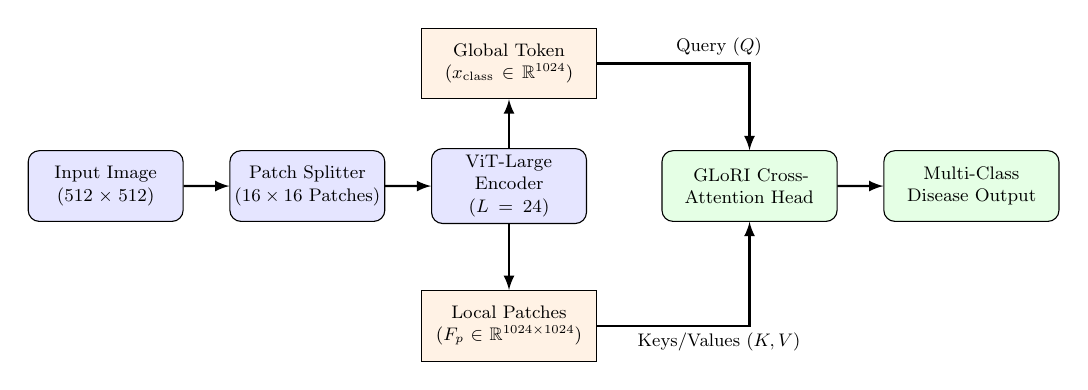
\begin{tikzpicture}[scale=0.73, transform shape, node distance=1.0cm and 0.8cm, auto, >=latex, font=\small]
		% Modern TikZ styles definition
		\tikzset{
			block/.style={rectangle, draw, fill=blue!10, text width=7em, text centered, rounded corners, minimum height=3.5em},
			cloud/.style={rectangle, draw, fill=green!10, text width=8em, text centered, rounded corners, minimum height=3.5em},
			process/.style={rectangle, draw, fill=orange!10, text width=8em, text centered, minimum height=3.5em}
		}
		
		% Row 1: Global Token Path (Top)
		\node [process] (cls) {Global Token\\($x_{\text{class}} \in \mathbb{R}^{1024}$)};
		
		% Row 2: Core Backbone Flow (Middle)
		\node [block, below=of cls, yshift=0.15cm] (vit) {ViT-Large\\Encoder ($L=24$)};
		\node [block, left=of vit] (patch) {Patch Splitter\\($16 \times 16$ Patches)};
		\node [block, left=of patch] (input) {Input Image\\($512 \times 512$)};
		
		\node [cloud, right=of vit, xshift=0.5cm] (glori) {GLoRI Cross-Attention Head};
		\node [cloud, right=of glori] (output) {Multi-Class\\Disease Output};
		
		% Row 3: Local Patches Path (Bottom)
		\node [process, below=of vit, yshift=-0.15cm] (patches) {Local Patches\\($F_p \in \mathbb{R}^{1024 \times 1024}$)};
		
		% Edges & Connections
		\draw [->, thick] (input) -- (patch);
		\draw [->, thick] (patch) -- (vit);
		
		% Routing from Encoder to the split rows
		\draw [->, thick] (vit) -- (cls);
		\draw [->, thick] (vit) -- (patches);
		
		% Routing from split rows into GLoRI module
		\draw [->, thick] (cls) -| node[pos=0.4, above] {Query ($Q$)} (glori);
		\draw [->, thick] (patches) -| node[pos=0.4, below] {Keys/Values ($K,V$)} (glori);
		
		\draw [->, thick] (glori) -- (output);
	\end{tikzpicture}
	\caption{Functional computational pipeline of the CheXFound framework: Transitioning from input image patch serialization, through the ViT-Large encoder blocks, to the GLoRI cross-attention alignment module.}
	\label{fig:chexfound_glori_flow}
\end{figure}

Furthermore, Figure~\ref{fig:chexfound_placeholder} serves as a modular architectural block diagram tracking the data flow from structural raw DICOM files to final predictions.

\begin{figure}[H]
	\centering
	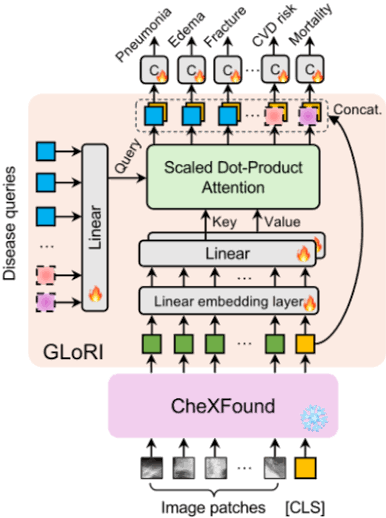
\includegraphics[width=\linewidth]{assets/vit-1.png}
	\caption{Modular schematic layout detailing parameter extraction, input token construction, and feature routing pathways between the frozen base model and the target task head.}
	\label{fig:chexfound_placeholder}
\end{figure}

\section{Medical Image Routing Model}
This section presents the proposed medical image routing model employed in the system and discusses the motivation behind the model, its problem formulation, and finally its architecture. This model serves as the decision-making unit of the system, where the destination of each input image is determined and forwarded thereafter.

\subsection{Motivation}
The increasing use of deep learning in medical image analysis has enabled the development of highly specialized models for tasks such as disease detection and diagnosis. In the context of lung cancer detection, chest X-ray and computed tomography (CT) images provide complementary diagnostic information and often require different processing pipelines and model architectures. While chest X-rays offer a low-cost and widely accessible imaging modality for preliminary screening, CT scans provide detailed cross-sectional information that supports more comprehensive assessment of lung abnormalities.

However, in real-world deployment scenarios, diagnostic systems are often exposed to heterogeneous image inputs originating from different imaging modalities, anatomical regions, or acquisition protocols. Applying a modality-specific diagnostic model to an inappropriate image type may lead to unreliable predictions and compromise the robustness and safety of the overall system. Consequently, there is a need for an initial classification mechanism capable of identifying the nature of incoming medical images before further analysis is performed.

This section introduces a medical image classification model designed to function as an image routing component within a larger lung cancer diagnostic pipeline. The model distinguishes between chest X-ray images, chest CT scan images, and an additional out-of-distribution category referred to as “Other.” By incorporating this third category, the system is able to explicitly handle images that do not belong to the intended diagnostic classes, thereby reducing the risk of misclassification and improving overall system reliability. Once classified, chest X-ray and CT scan images are forwarded to their corresponding lung cancer diagnostic models, while out-of-distribution images are rejected from further analysis. The following subsections present the motivation for this approach, formally define the classification problem, and describe the model architecture employed.

\subsection{Problem Statement}

The goal of this work is to develop an automated medical image classification model capable of identifying the type of an input image and routing it to the appropriate downstream analysis. The task is formulated as a three-class classification problem, where each input image \(X \in \mathbb{R}^{224 \times 224 \times 3}\) must be assigned to one of three categories: chest X-ray images (\(0\)), chest CT scan images (\(1\)), or out-of-distribution images labeled as \emph{Other} (\(2\)). This multi-class formulation ensures that irrelevant or ambiguous inputs are explicitly handled, improving system safety and reducing the risk of inappropriate downstream processing.

The model is designed to output a probability distribution \(\mathbf{p} = [p_0, p_1, p_2]\) over the three classes, where \(p_k = P(y = k \mid X)\) and \(\sum_{k=0}^{2} p_k = 1\). The predicted class is obtained by selecting the class with the highest probability, \(\hat{y} = \arg\max_{k} p_k\). Images classified as chest X-rays are forwarded to the X-ray-based lung cancer detection model, while images classified as CT scans are routed to the CT-based lung cancer detection model. By incorporating the \emph{Other} category, the model avoids forcing all inputs into diagnostic categories and can robustly separate images outside the target distribution, laying a solid foundation for safe integration within a larger medical image analysis pipeline.

\subsection{Model Architecture}

The proposed medical image classification model is designed using a transfer learning approach based on the ResNet50 convolutional neural network. The architecture follows a structured pipeline consisting of input preprocessing, deep feature extraction, feature aggregation, and final classification. This modular design allows the model to benefit from representations learned on large-scale image datasets while adapting effectively to the target medical imaging task. An overview of the complete classification pipeline is illustrated in Figure~\ref{fig:overall_architecture}.

\begin{figure}[h]
	\centering
	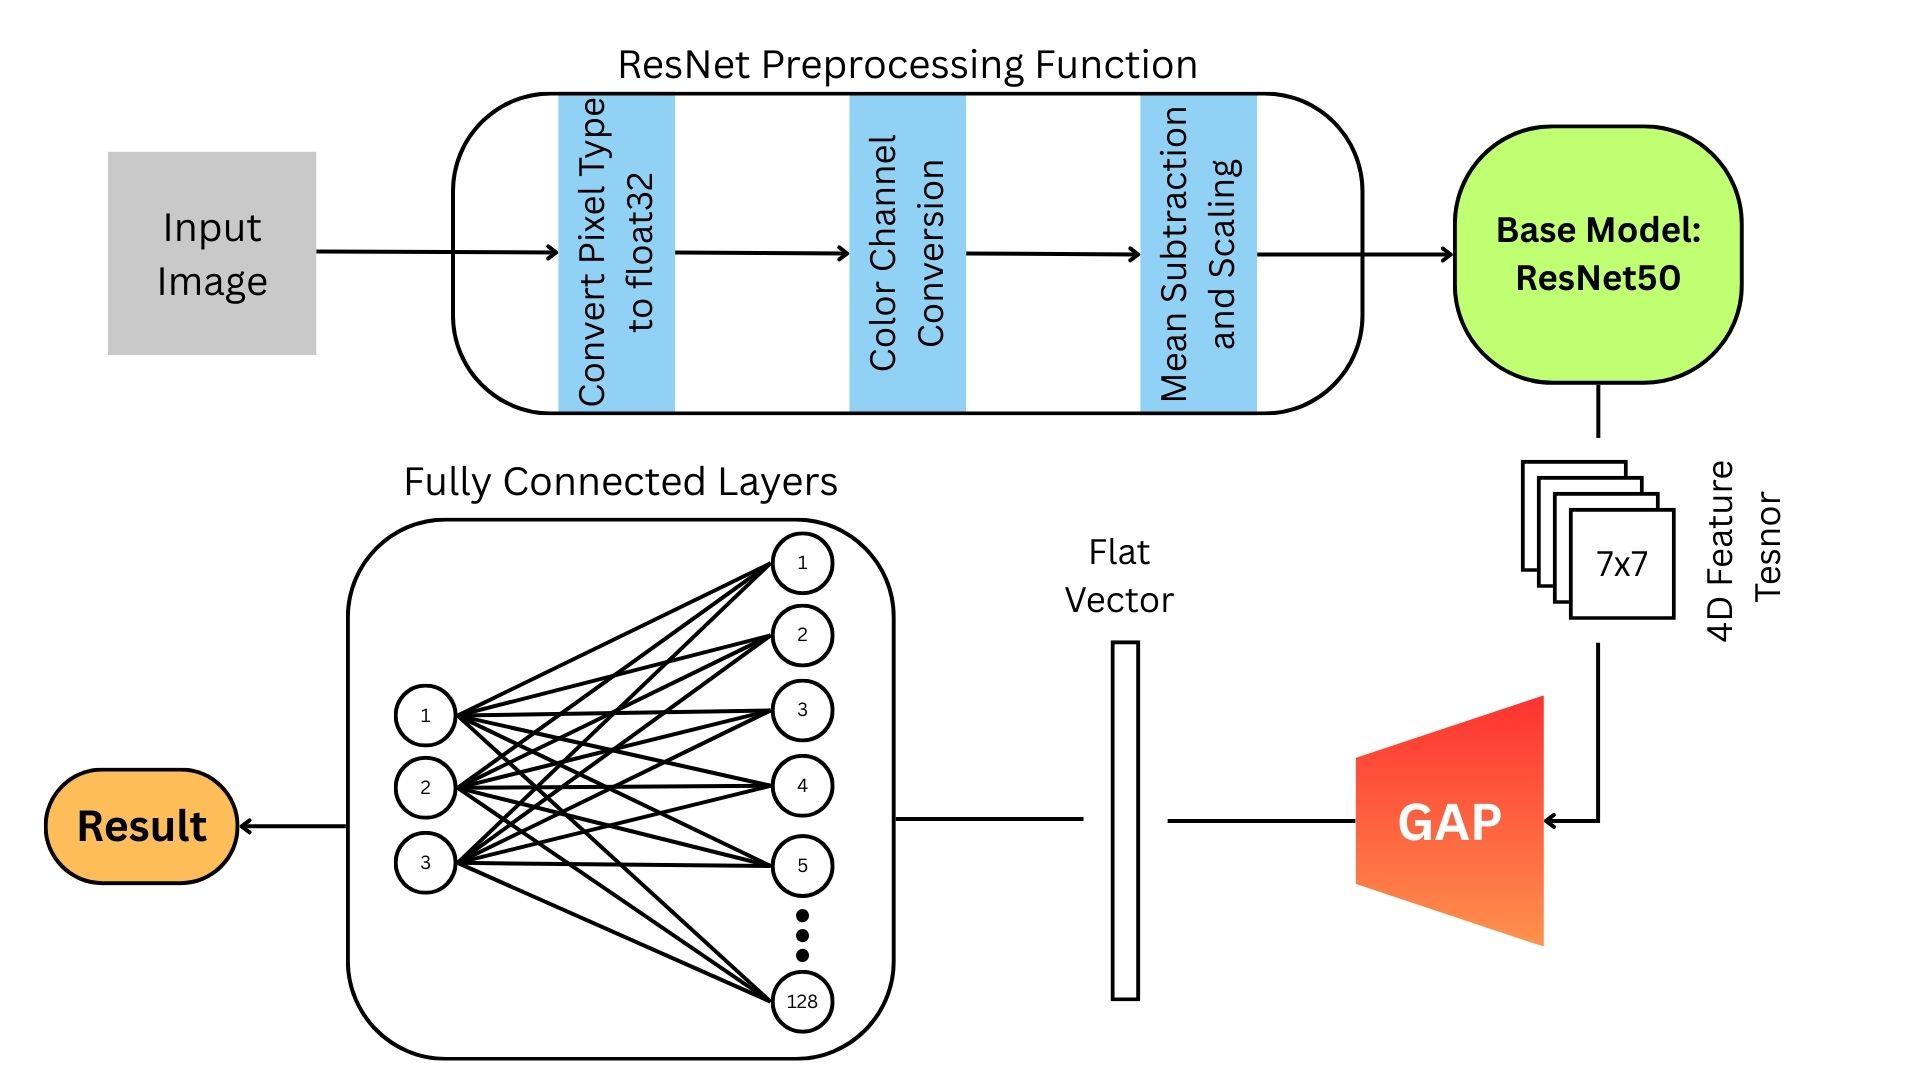
\includegraphics[width=0.95\linewidth]{assets/router-architecture.jpg}
	\caption{Overall architecture of the proposed medical image routing model.}
	\label{fig:overall_architecture}
\end{figure}

The input to the model is a medical image \(X \in \mathbb{R}^{224 \times 224 \times 3}\), resized to a fixed spatial resolution and represented in RGB color space. Prior to being processed by the pretrained network, the image undergoes a preprocessing step to ensure compatibility with the ResNet50 weights. This step mirrors the preprocessing applied during the original ImageNet training of ResNet50 and is essential for effective transfer learning. Specifically, the input image is first converted to floating-point representation, its color channels are reordered from RGB to BGR, and a fixed channel-wise mean is subtracted. Let \(X_{rgb}\) denote the raw input image; the preprocessed image \(X_{prep}\) is obtained as \(X_{prep} = \mathrm{BGR}(X_{rgb}) - \mu\), where \(\mu = [103.939, 116.779, 123.68]\) represents the ImageNet mean for the blue, green, and red channels, respectively. This operation centers the input distribution around zero and aligns it with the statistical properties expected by the pretrained backbone.

Following preprocessing, the image is passed through the ResNet50 network with its original classification layers removed. In this configuration, ResNet50 functions as a fully convolutional feature extractor. For an input tensor of shape \((224, 224, 3)\), the output of the backbone is a high-dimensional feature map of shape \((7, 7, 2048)\). This tensor contains 2048 feature channels, each encoding abstract visual patterns such as anatomical structures, textures, and modality-specific characteristics while preserving coarse spatial relationships within the image. For a detailed discussion of the ResNet50 model architecture, refer to Subsection~\ref{subsec:resnet50-arch}.

To transform the spatial feature maps into a compact representation suitable for classification, a global average pooling operation is applied to the output of the ResNet50 backbone. This operation computes the average activation of each feature channel across the spatial dimensions, effectively summarizing the presence of each learned feature over the entire image. Given a feature map \(F \in \mathbb{R}^{7 \times 7 \times 2048}\), the pooled feature vector \(z \in \mathbb{R}^{2048}\) is computed such that each element \(z_k\) corresponds to the mean of the activations in channel \(k\), i.e.
\begin{equation*}
	z_k = \frac{1}{7 \times 7} \sum_{i=1}^{7} \sum_{j=1}^{7} F_{i,j,k}
\end{equation*}
This operation reduces the tensor shape from \((7, 7, 2048)\) to \((2048)\) while significantly lowering the number of parameters required in subsequent layers and improving generalization.

The resulting feature vector is then passed to a task-specific classification head composed of fully connected layers. These layers learn discriminative combinations of the extracted features and map them to the target class space. The final layer applies a softmax activation function, producing a probability distribution \(\mathbf{p} = [p_0, p_1, p_2]\), where each component represents the predicted probability of the image belonging to the chest X-ray class, chest CT scan class, or the out-of-distribution \emph{Other} class. The predicted label is obtained as \(\hat{y} = \arg\max_k p_k\).


\section{Chest Disease Classification Model}

This section presents one of the downstream diagnostic models developed within the project, focusing on automated multi-class classification of chest diseases from chest X-ray (CXR) images. The model is designed as a robust and interpretable pipeline that integrates standardized image preprocessing, lung region isolation, and deep learning–based classification using transfer learning. Emphasis is placed on architectural design choices and methodological foundations rather than performance evaluation, which is discussed in a later chapter.

\subsection{Motivation}

Deep learning has demonstrated strong potential in medical image analysis, yet several challenges remain, including variability in image acquisition, class imbalance, and the need for explainable decision-making. The proposed model addresses these issues through a multi-stage pipeline that enhances image quality, isolates clinically relevant lung regions, and applies a transfer learning–based classifier augmented with explainability techniques.

\subsection{Problem Statement}

The objective of this model is to perform multi-class classification of chest X-ray images into the following diagnostic categories:
\[
\mathcal{C} = \{\text{NORMAL}, \text{PNEUMONIA}, \text{COVID-19}, \text{TUBERCULOSIS}\}.
\]

Given an input chest X-ray image \( I \in \mathbb{R}^{H \times W} \), the task is to learn a mapping
\[
f_\theta : I \rightarrow \mathbf{p},
\]
where \( \mathbf{p} \in \mathbb{R}^{|\mathcal{C}|} \) is a probability distribution over disease classes and \( \theta \) denotes the model parameters.

To improve robustness and clinical relevance, the classification task is constrained to lung parenchyma regions extracted via an explicit segmentation stage. Additionally, the model must provide interpretable outputs to support clinical trust, motivating the use of gradient-based visualization techniques.

\subsection{Model Architecture}

The diagnostic model is structured as a multi-stage pipeline, illustrated conceptually in Figure~\ref{fig:chest_pipeline_overview}. The pipeline consists of three main components: image preprocessing, lung segmentation, and disease classification.


\begin{figure}[h]
	\centering
	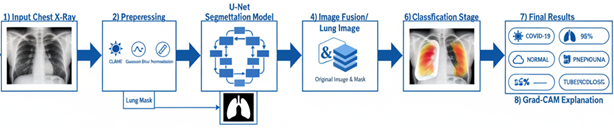
\includegraphics[width=0.75\textwidth]{assets/chest-pipeline.png}
	\caption{High-level overview of the multi-stage chest disease classification pipeline.}
	\label{fig:chest_pipeline_overview}
\end{figure}


Each chest X-ray image undergoes a standardized preprocessing pipeline to enhance diagnostically relevant features. Images are first converted to grayscale and enhanced using Contrast Limited Adaptive Histogram Equalization (CLAHE). Noise introduced during enhancement is mitigated using Gaussian smoothing with a \(5 \times 5\) kernel.

Pixel intensities are then normalized using Min--Max normalization: $I_{\text{norm}} = \frac{I - I_{\min}}{I_{\max} - I_{\min}}$ where \( I_{\min} \) and \( I_{\max} \) represent the minimum and maximum pixel values of the image. Finally, images are converted to RGB format to ensure compatibility with the ResNet50 model. For a discussion of the ResNet50 model, refer to Subsection~\ref{subsec:resnet50-arch}.

Figure~\ref{fig:preprocessing} illustrates the effect of the preprocessing pipeline on representative CXR images.

\begin{figure}[h]
	\centering
	\begin{subfigure}[b]{0.25\textwidth}
		\centering
		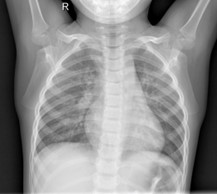
\includegraphics[width=\textwidth]{assets/pneu1.jpg}
		\caption{Original Pneumonia CXR}
		\label{fig:orig-pneumonia}
	\end{subfigure}
	\hspace*{1cm}
	\begin{subfigure}[b]{0.25\textwidth}
		\centering
		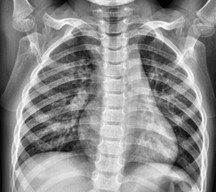
\includegraphics[width=\textwidth]{assets/proc-pneu1.jpg}
		\caption{Preprocessed Pneumonia CXR}
		\label{fig:proc-pneumonia}
	\end{subfigure}
	\\
	\begin{subfigure}[b]{0.25\textwidth}
		\centering
		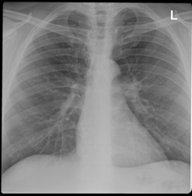
\includegraphics[width=\textwidth]{assets/pneu2.png}
		\caption{Original Pneumonia CXR}
		\label{fig:orig-pneumonia2}
	\end{subfigure}
	\hspace*{1cm}
	\begin{subfigure}[b]{0.25\textwidth}
		\centering
		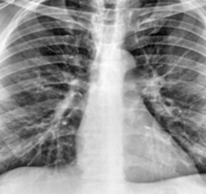
\includegraphics[width=\textwidth]{assets/proc-pneu2.png}
		\caption{Preprocessed Pneumonia CXR}
		\label{fig:proc-pneumonia2}
	\end{subfigure}
	\caption{Chest X-ray images before and after preprocessing, highlighting improved contrast and reduced noise.}
	\label{fig:preprocessing}
\end{figure}
%	\begin{figure}[h]
	%		\centering
	%		\includegraphics[width=0.9\textwidth]{preprocessing_comparison.png}
	%		\caption{Chest X-ray images before and after preprocessing, highlighting improved contrast and reduced noise.}
	%		\label{fig:preprocessing}
	%	\end{figure}

To ensure that classification focuses exclusively on clinically relevant regions, a U-Net–based segmentation model is employed to extract lung masks. The U-Net architecture follows an encoder–decoder structure with skip connections that preserve spatial information, making it well suited for biomedical image segmentation. The U-Net architecture used is shown in Figure~\ref{fig:unet-arch}



\begin{figure}[h]
	\centering
	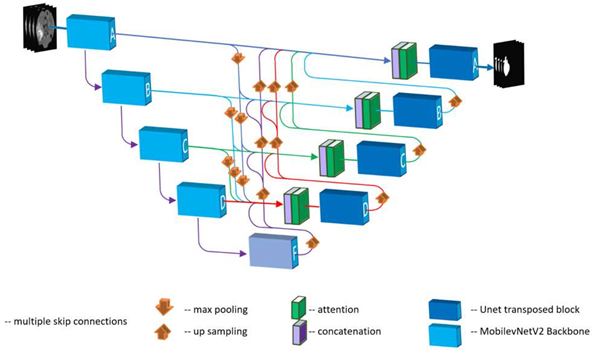
\includegraphics[width=0.9\textwidth]{assets/unet-arch.png}
	\caption{The U-Net architecture, illustrating the encoder-decoder structure with skip connections that merge high-resolution features from the contracting path with upsampled features in the expansive path. This design is highly effective for precise medical image segmentation.}
	\label{fig:unet-arch}
\end{figure}

The segmentation network outputs a binary lung mask \( M \in \{0,1\}^{H \times W} \), which is applied to the preprocessed image using element-wise multiplication:
\[
I_{\text{lung}} = I_{\text{norm}} \odot M.
\]

Training of the segmentation model is guided by the Dice Loss, derived from the Dice--Sørensen Coefficient (DSC):
\[
\text{DSC} = \frac{2|X \cap Y|}{|X| + |Y|},
\]
where \( X \) and \( Y \) denote the predicted and ground-truth masks, respectively. The loss function is defined as
\[
\mathcal{L}_{\text{Dice}} = 1 - \text{DSC},
\]
which is particularly effective in handling class imbalance between lung and background pixels. The result of using segmentation on CXR images is illustrated in Figure~\ref{fig:lung_segmentation}

\begin{figure}[h]
	\centering
	\begin{subfigure}[b]{0.25\textwidth}
		\centering
		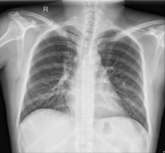
\includegraphics[width=\textwidth]{assets/proc-cxr.png}
		\caption{Preprocessed CXR Image}
		\label{fig:proc-cxr}
	\end{subfigure}
	\hspace*{1cm}
	\begin{subfigure}[b]{0.25\textwidth}
		\centering
		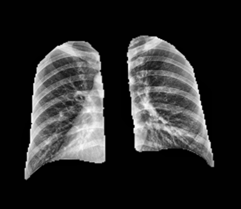
\includegraphics[width=\textwidth]{assets/segmented-lung.png}
		\caption{Segmented Lung Image after Mask Application}
		\label{fig:segmented-lung}
	\end{subfigure}
	\caption{Application of the U-Net segmentation mask. The original preprocessed Figure~\ref{fig:proc-cxr} is processed to produce the final segmented lung Figure~\ref{fig:segmented-lung}, which serves as the input for the classification stage}
	\label{fig:lung_segmentation}
\end{figure}

%	\begin{figure}[h]
	%		\centering
	%		\includegraphics[width=0.9\textwidth]{lung_segmentation.png}
	%		\caption{Application of the U-Net segmentation mask to isolate lung regions from chest X-ray images.}
	%		\label{fig:lung_segmentation}
	%	\end{figure}
%	
The final classification stage employs a ResNet50-based transfer learning model. ResNet architectures leverage residual connections to facilitate gradient flow and enable the training of deep networks. As the ResNet family is discussed in detail earlier in this book, only a brief overview is provided here.

A ResNet50 model pre-trained on ImageNet is used as a feature extractor, with early layers frozen to preserve general visual representations. A custom classification head is appended, consisting of global average pooling, fully connected layers with ReLU activation, dropout for regularization, and a final softmax layer producing class probabilities.

The model is trained using Sparse Categorical Cross-Entropy loss:
\[
\mathcal{L}_{\text{CE}} = - \sum_{i=1}^{N} \log p_{i,c},
\]
where \( p_{i,c} \) denotes the predicted probability of the true class \( c \) for sample \( i \). To address class imbalance, class-weighted loss scaling is applied during training.

To enhance interpretability, Gradient-weighted Class Activation Mapping (Grad-CAM) is employed to visualize the regions most influential to model predictions, an example is shown in Figure~\ref{fig:gradcam}. Grad-CAM computes the gradients of the target class score with respect to the feature maps of the final convolutional layer and produces a coarse localization map highlighting salient regions.

These heatmaps are overlaid on the original chest X-ray images, enabling qualitative assessment of whether the model attends to clinically meaningful lung regions.

\begin{figure}[h]
	\centering
	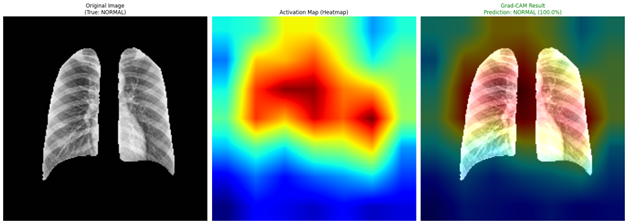
\includegraphics[width=0.9\textwidth]{assets/gradcam.png}
	\caption{Grad-CAM visualizations highlighting regions contributing to model predictions.}
	\label{fig:gradcam}
\end{figure}


\section{Lung Cancer Detection Model}
This section presents the lung cancer and tuberculosis detection model developed within the project, focusing on automated localization and classification of pulmonary abnormalities from chest X-ray (CXR) images[cite: 1, 2]. The model is designed as an end-to-end object detection pipeline that integrates binary mask conversion, bounding box generation, and deep learning–based detection using the YOLOv8 architecture[cite: 3]. Emphasis is placed on the data preparation strategy and architectural design choices that underpin the detection framework[cite: 4].

\subsection{Motivation}
Object detection frameworks offer distinct advantages over image-level classification for medical imaging tasks, as they provide explicit spatial localization of pathological regions rather than a single diagnostic label[cite: 5, 6]. For lung cancer and tuberculosis screening, identifying the precise location and extent of pulmonary lesions or infiltrates is clinically essential, as it directly informs radiological assessment and subsequent clinical decision-making[cite: 7]. The proposed model addresses this requirement by reformulating the diagnostic task as a bounding box regression and classification problem, enabling simultaneous localization and identification of disease regions within a single unified forward pass[cite: 8].

\subsection{Problem Statement}
The objective of this model is to perform multi-class detection of pulmonary abnormalities in chest X-ray images, identifying and localizing instances belonging to the following diagnostic categories[cite: 9, 10]:
\begin{equation}
	C = \{\text{tumor}, \text{tuberculosis}\} [cite: 11]
\end{equation}

Given an input chest X-ray image $I \in \mathbb{R}^{H \times W}$, the task is to learn a mapping[cite: 12]:
\begin{equation}
	f_\theta : I \rightarrow \{(b_i, c_i, s_i)\}_{i=1 \dots N} [cite: 13]
\end{equation}
where each tuple $(b_i, c_i, s_i)$ denotes the predicted bounding box coordinates, class label, and confidence score for the $i$-th detected region, and $\theta$ represents the model parameters[cite: 14].

To bridge the gap between pixel-level segmentation annotations (binary masks) and the bounding box representation required by the detection framework, an explicit mask-to-box conversion stage is incorporated as the first step of the pipeline[cite: 15]. Each connected foreground component in the binary annotation mask is converted into a normalized YOLO-format bounding box, enabling the use of richly annotated mask datasets for detection training without manual re-labeling[cite: 16].

\subsection{Model Architecture}
The detection model is structured as a three-stage pipeline consisting of: (1) mask-to-bounding-box conversion and dataset preparation, (2) YOLO-format data organization and configuration, and (3) YOLOv8-based detection model training and evaluation[cite: 17, 18]. Each stage is described in detail below[cite: 19].

\begin{figure}[htbp]
	\centering
	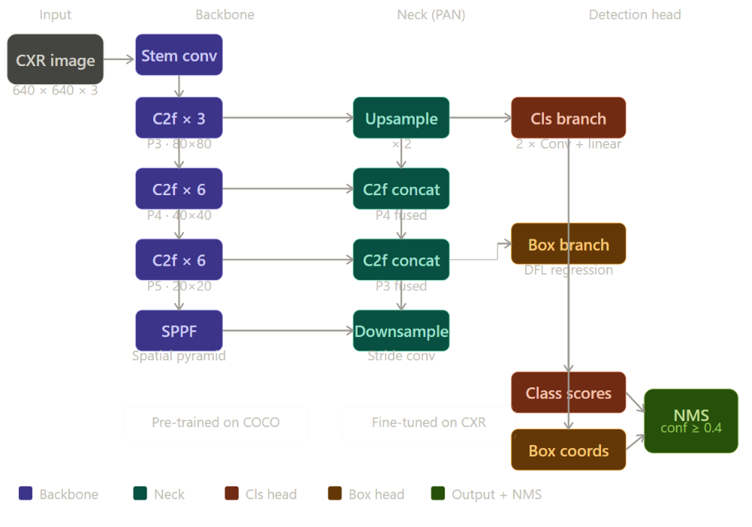
\includegraphics[width=\textwidth]{assets/yolo8_arch.png}
	\caption{YOLOv8 architecture pipeline for automated localization and classification of pulmonary abnormalities.}
	\label{fig:yolov8_architecture}
\end{figure}

\subsubsection{Mask-to-Bounding-Box Conversion}
Annotation masks for pulmonary lesions are provided as binary PNG images in which foreground pixels (intensity $> 127$) correspond to pathological regions[cite: 20, 21]. To convert these masks into YOLO-format bounding box annotations, connected component analysis is applied using external contour detection[cite: 22]. For each detected contour, an axis-aligned bounding box is computed and normalized with respect to the image dimensions, yielding center coordinates and extent values in the range $[0, 1]$[cite: 23].

Formally, for a contour with pixel-space bounding rectangle $(x, y, w, h)$ within an image of width $W$ and height $H$, the normalized YOLO representation is[cite: 24]:
\begin{equation}
	c_x = \frac{x + w/2}{W}, \quad c_y = \frac{y + h/2}{H}, \quad n_w = \frac{w}{W}, \quad n_h = \frac{h}{H} [cite: 25]
\end{equation}

Contours enclosing fewer than 5 pixels in either dimension are discarded as noise prior to annotation generation[cite: 26]. All foreground components within a given mask are assigned the class index corresponding to the image-level label (tumor or tuberculosis), since mask annotations are provided per diagnostic category[cite: 27].

\subsubsection{Dataset Preparation and Splitting}
Following bounding box conversion, the dataset is partitioned into training, validation, and test subsets using stratified random splitting[cite: 28, 29]. The default split proportions are 75\% training, 15\% validation, and 10\% test, with random seed fixed at 42 to ensure reproducibility[cite: 30]. Image files and their corresponding YOLO label files are organized into the standard YOLO directory structure, with separate image and label folders for each split[cite: 31]. A YAML configuration file is generated automatically to specify dataset paths, the number of classes, and class names, serving as the interface between the prepared dataset and the YOLOv8 training framework[cite: 32].

\subsubsection{YOLOv8 Detection Architecture}
Object detection is performed using YOLOv8, the latest generation of the You Only Look Once (YOLO) family of single-stage detectors[cite: 33, 34]. YOLOv8 follows an anchor-free design and adopts a CSPDarknet backbone for feature extraction, a Path Aggregation Network (PAN) neck for multi-scale feature fusion, and a decoupled detection head that separately predicts classification scores and bounding box offsets[cite: 35]. This design enables real-time inference while maintaining competitive localization accuracy[cite: 36].

A YOLOv8n (nano) variant is employed as the base model, pre-trained on the COCO dataset, and fine-tuned on the prepared CXR detection dataset[cite: 37]. The model is trained for 50 epochs with an input resolution of $640 \times 640$ pixels and a batch size of 16[cite: 38]. Transfer learning is leveraged by initializing all network weights from the COCO pre-trained checkpoint, with all layers unfrozen to allow domain-specific adaptation[cite: 38]. The training objective combines binary cross-entropy loss for classification, distribution focal loss (DFL) for bounding box regression, and a complete intersection-over-union (CIoU) penalty term to improve localization precision[cite: 39]:
\begin{equation}
	L = \lambda_{\text{cls}} \cdot L_{\text{cls}} + \lambda_{\text{box}} \cdot L_{\text{box}} + \lambda_{\text{dfl}} \cdot L_{\text{DFL}} [cite: 40]
\end{equation}
where $\lambda_{\text{cls}}$, $\lambda_{\text{box}}$, and $\lambda_{\text{dfl}}$ are scalar weighting coefficients that balance the contribution of each loss component during optimization[cite: 41].

After training, the best-performing checkpoint, selected based on validation mean Average Precision at IoU threshold 0.50 (mAP50), is retained for evaluation[cite: 42]. Model performance is assessed on both the held-out validation and test splits, reporting mAP50, mAP50–95, precision, and recall as primary evaluation metrics[cite: 43]. Qualitative evaluation is conducted by visually inspecting annotated predictions on test set images, examining the spatial correspondence between predicted bounding boxes and known pathological regions[cite: 44].

\begin{figure}[htbp]
	\centering
	\begin{minipage}{0.48\textwidth}
		\centering
		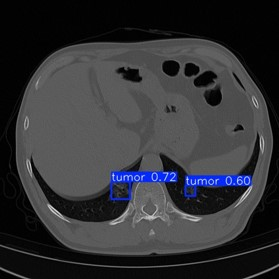
\includegraphics[width=\textwidth]{assets/lung1.jpg}
		\caption{Qualitative evaluation showing tumor localization (confidence scores 0.72 and 0.60) on an axial CT slice.}
		\label{fig:qualitative_ct_1}
	\end{minipage}\hfill
	\begin{minipage}{0.48\textwidth}
		\centering
		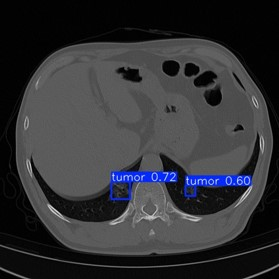
\includegraphics[width=\textwidth]{assets/lung1.jpg}
		\caption{Qualitative evaluation showing tumor localization (confidence score 0.87) on an axial CT slice.}
		\label{fig:qualitative_ct_2}
	\end{minipage}
\end{figure}

\subsection{Interpretability Considerations}
Unlike classification-only models that require post-hoc gradient visualization to identify diagnostically relevant regions, the detection framework provides explicit spatial outputs in the form of bounding boxes and associated confidence scores[cite: 45, 46]. Each prediction directly encodes the model's estimate of where a pathological region is located and how confident it is in that localization[cite: 47]. This built-in spatial explainability reduces the reliance on auxiliary interpretability methods and aligns more naturally with clinical reporting conventions, in which radiologists annotate specific anatomical regions rather than assigning image-level labels[cite: 48]. Confidence thresholding ($\tau = 0.4$) and non-maximum suppression with an IoU threshold of 0.6 are applied at inference time to filter low-quality or redundant detections, producing a concise set of high-confidence predictions per image[cite: 49].

\begin{figure}[htbp]
	\centering
	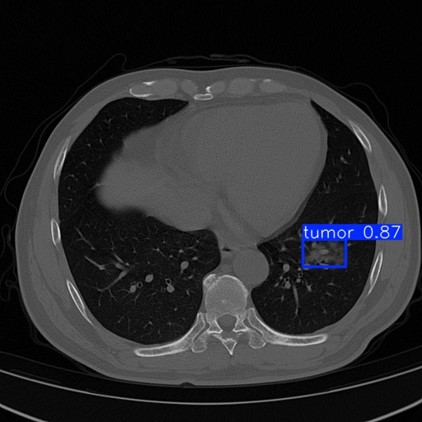
\includegraphics[width=0.6\textwidth]{assets/lung3.jpg}
	\caption{Example of an interpretable YOLO detection result on a chest CT image. The model localizes a suspected lesion using a bounding box and reports a confidence score of 0.87. Such spatial predictions provide inherent interpretability by explicitly identifying the anatomical region associated with the model's decision, reducing the need for post-hoc visualization techniques.}
	\label{fig:interpretability_example}
\end{figure}
\FloatBarrier
\section{Federated Learning}
\subsection{Concept and Motivation}
\label{subsec:fl_concept}
 
Federated learning (FL) is a distributed machine learning paradigm in which
a model is trained collaboratively across multiple independent nodes without
any raw data leaving its source institution~\cite{mcmahan2017}. Rather than
centralizing training samples on a shared server, FL brings the computation
to the data: each participating node trains a local model on its private
dataset and shares only the resulting model parameters with a central
aggregation server, which combines the updates into an improved global model.
This cycle repeats for a defined number of communication rounds until the
global model converges.
 
The motivation for adopting FL in this work is rooted in the fundamental
tension between data-driven model development and patient privacy. Healthcare
institutions collect large volumes of annotated medical images, yet regulatory
frameworks --- including the Health Insurance Portability and Accountability Act
(HIPAA) in the United States and the General Data Protection Regulation (GDPR)
in the European Union --- impose strict constraints on cross-institutional data
sharing. Negotiating data transfer agreements is costly, time-consuming, and
in many cases legally impractical. FL resolves this tension by enabling
institutions to contribute to a shared model without relinquishing data
custody, making large-scale collaborative medical AI both legally feasible
and technically practical.
 
% -----------------------------------------------------------------------------
\subsection{Federated Learning in Medical Imaging}
\label{subsec:fl_medical}
 
The adoption of FL in the medical domain has grown substantially since its
introduction, driven by the recognition that many clinical datasets are too
small at any single institution to train robust deep learning models, while
the combined data across institutions would be sufficient~\cite{sheller2019}.
FL directly addresses this data insufficiency problem without requiring
physical data consolidation.
 
In medical imaging specifically, FL has been applied across a broad range of
modalities and anatomical targets. Early work by Sheller~\textit{et al.}
demonstrated FL for brain tumor segmentation from MRI scans across multiple
institutions, achieving performance comparable to centralized training without
sharing any patient data~\cite{sheller2019}. Subsequent studies have extended
FL to chest radiograph classification, diabetic retinopathy screening from
fundus photography, histopathology slide analysis, and cardiac structure
segmentation from echocardiography, among others~\cite{rieke2020}.
 
This breadth of applicability is a key motivation for the design of the
proposed system. Rather than building a solution tied to a specific model
architecture or anatomical region, the FL framework developed in this work
is designed to be \textbf{model-agnostic} and \textbf{organ-agnostic}: any
classification or segmentation backbone can be substituted as the local
model, and the training data can comprise images from any body region or
imaging modality. The federated coordination layer — covering client
management, weight aggregation, and communication — remains unchanged
regardless of the underlying clinical task.
 
% -----------------------------------------------------------------------------
\subsection{The Federated Averaging Algorithm}
\label{subsec:fedavg}
 
The aggregation algorithm that underpins the proposed system is Federated
Averaging (FedAvg), introduced by McMahan~\textit{et al.}~\cite{mcmahan2017}
and the most widely adopted FL optimization method to date. FedAvg operates
in iterative communication rounds. Let $K$ denote the number of participating
clients, $\mathcal{D}_k$ the private dataset of client $k$, $n_k =
|\mathcal{D}_k|$ its size, and $n = \sum_{k=1}^{K} n_k$ the total number of
training samples across all clients. The global model at round $t$ is
parameterized by weight vector $\mathbf{w}_t$. Each round consists of three
phases:
 
\textbf{(1) Broadcast.} The server distributes the current global model
weights to all $K$ clients:
\begin{equation}
    \mathbf{w}_t \;\longrightarrow\; \{\text{client}_1, \dots, \text{client}_K\}.
\end{equation}
\textbf{(2) Local Training.} Each client $k$ independently minimizes its
local empirical risk $\mathcal{L}_k$ over $E$ local epochs using a gradient-
based optimizer, producing updated local weights:
\begin{equation}
    \mathbf{w}_t^k \;=\; \mathbf{w}_t \;-\; \eta\,\nabla\mathcal{L}_k(\mathbf{w}_t),
\end{equation}
where $\eta$ is the local learning rate and $\mathcal{L}_k$ is the
task-specific loss function evaluated over the client's local dataset:
\begin{equation}
    \mathcal{L}_k(\mathbf{w}) \;=\;
    \frac{1}{n_k}\sum_{(x_i,\,y_i)\,\in\,\mathcal{D}_k}
    \ell\!\left(f_{\mathbf{w}}(x_i),\,y_i\right).
\end{equation}
 
\textbf{(3) Aggregation.} The server collects the locally updated weights
from all clients and computes the new global model as a weighted average
proportional to each client's dataset size:
\begin{equation}
    \mathbf{w}_{t+1} \;=\; \sum_{k=1}^{K}\frac{n_k}{n}\,\mathbf{w}_t^k.
    \label{eq:fedavg}
\end{equation}
This process minimizes the global objective:
\begin{equation}
    F(\mathbf{w}) \;=\; \sum_{k=1}^{K}\frac{n_k}{n}\,\mathcal{L}_k(\mathbf{w}).
\end{equation}
Equation~\eqref{eq:fedavg} assigns greater influence to clients with larger
datasets, which is appropriate in the medical setting where institutional
dataset sizes vary considerably. Clients contributing more annotated images
should exert proportionally greater influence on the global model.
 
% -----------------------------------------------------------------------------
\subsection{Key Parameters of a Federated Learning System}
\label{subsec:fl_parameters}
 
Configuring a federated learning system involves a distinct set of
parameters beyond those of conventional deep learning. These parameters
govern the coordination between server and clients and directly affect
convergence speed, model quality, communication cost, and privacy. A clear
understanding of each parameter is essential for adapting the system to
different clinical tasks. Table~\ref{tab:fl_params} provides an overview
of the critical parameters and their implications.
 
\begin{table}[!htbp]
\centering
\caption{Key Federated Learning Parameters and Their Clinical Implications}
\label{tab:fl_params}
\begin{tabular}{|p{3.2cm}|p{4.2cm}|p{5.8cm}|}
\hline
\textbf{Parameter} & \textbf{Definition} & \textbf{Implication} \\
\hline
Number of clients ($K$)
    & Total participating institutions
    & More clients improve data diversity and model generalization but
      increase coordination overhead. \\
\hline
Communication rounds ($T$)
    & Number of server--client training cycles
    & More rounds improve accuracy at the cost of higher communication
      volume. Convergence is typically monitored to select $T$. \\
\hline
Client fraction ($C$)
    & Proportion of clients selected per round ($C \in (0,1]$)
    & $C = 1.0$ uses all clients every round (synchronous FL).
      $C < 1.0$ enables asynchronous, scalable training. \\
\hline
Local epochs ($E$)
    & Training epochs each client performs before returning weights
    & Higher $E$ reduces communication rounds but risks \textit{client drift}
      — divergence of local models due to non-IID data~\cite{li2020}. \\
\hline
Local batch size ($B$)
    & Mini-batch size for local gradient computation
    & Affects local convergence speed, memory footprint, and gradient
      privacy (smaller batches increase reconstruction attack risk). \\
\hline
Local learning rate ($\eta$)
    & Step size for local gradient updates
    & Must be tuned per model architecture; too large a value exacerbates
      client drift in non-IID settings. \\
\hline
Aggregation strategy
    & Algorithm used to combine client updates (e.g., FedAvg, FedProx,
      FedNova)
    & Choice depends on data heterogeneity; FedAvg is the standard baseline;
      FedProx adds a proximal term to limit client drift. \\
\hline
Data partitioning scheme
    & How training data is divided across clients (IID vs. non-IID)
    & Non-IID partitions (realistic in healthcare) slow convergence and
      reduce final accuracy compared to IID partitions. \\
\hline
Minimum clients for aggregation
    & Minimum number of client updates required before the server aggregates
    & Prevents the global model from being updated on insufficient
      information; critical for stability. \\
\hline
\end{tabular}
\end{table}
 
Among these, the number of local epochs $E$ and the aggregation strategy
warrant particular attention in the medical imaging context. Increasing $E$
reduces the number of costly communication rounds, which is beneficial in
healthcare networks where bandwidth and uptime may be limited. However,
when client datasets are statistically heterogeneous — a common condition
across hospitals using different scanners, populations, or labeling protocols
— high $E$ causes the local models to overfit to their local distributions
and diverge from the global optimum, a phenomenon known as \textit{client
drift}~\cite{li2020}. The selection of $E$ therefore requires careful
empirical tuning for each deployment scenario.
 
% -----------------------------------------------------------------------------
\subsection{System Architecture Overview}
\subsubsection{Client--Server Design}

The system follows a two-tier federated learning architecture implemented using the Flower (\texttt{flwr}) framework. A single Federated Learning (FL) Server process hosts both the Flower gRPC server and a FastAPI-based REST management API within the same Python process. The Flower server operates on port \texttt{50051}, while the REST management layer operates on port \texttt{8001}. Both services share a common \texttt{SharedState} singleton object that stores the current round status, active model type, round identifier, and the reference to the active Flower thread. This co-location eliminates additional network overhead between the aggregation engine and the management layer and enables efficient coordination between both services.

Each participating hospital deploys an FL Client as a Docker container. Upon startup, the client continuously polls the server's health endpoint until a federated learning round becomes active. Once the server signals round activation, the client initializes the appropriate model according to the task being executed. For any task a client model is instantiated. The client subsequently waits for the gRPC service to become available before connecting through Flower's \texttt{NumPyClient} interface.

A key design principle of the architecture is data locality. Medical images and patient records remain exclusively within the hospital infrastructure and are never transmitted to the central server. Instead, only serialized NumPy arrays containing model parameters are exchanged during federated learning rounds. This design significantly reduces privacy risks while maintaining collaborative model training across institutions.

\begin{figure}[H]
	\centering
	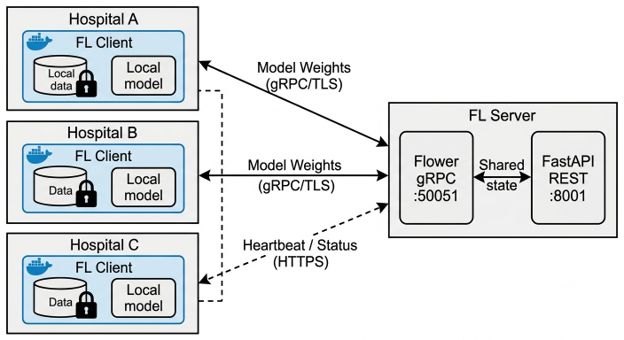
\includegraphics[width=0.9\textwidth]{assets/fl_system_architecture.png}
	\caption{Two-tier federated learning system architecture. Hospital clients communicate with the central federated learning server through TLS-secured gRPC channels, while the REST management layer provides round lifecycle management and monitoring. Raw medical data remains within each hospital boundary.}
	\label{fig:fl_system_architecture}
\end{figure}

\subsubsection{Communication Protocol}

All model parameter exchanges between federated learning clients and the central server are performed using gRPC, Google's high-performance remote procedure call framework built on HTTP/2 and Protocol Buffers. The Flower framework serializes model weight tensors into Protocol Buffer messages before transmission, providing an efficient and platform-independent communication mechanism.

To ensure secure communication, the production deployment uses Transport Layer Security (TLS). Before any model parameters are exchanged, a complete TLS handshake is performed involving a trusted Certificate Authority (CA) certificate, a server certificate, and the server's private key. This process guarantees encrypted communication channels and prevents unauthorized interception or modification of model updates during transmission.

In addition to the gRPC communication channel, the system incorporates a secondary REST-based heartbeat mechanism. Each client periodically sends status reports to the FastAPI management API at a configurable interval, with a default period of 15 seconds. These heartbeat messages include metadata such as the currently active model type and the active federated learning round identifier.

The heartbeat channel provides real-time visibility into client participation and system health while maintaining patient privacy. No medical images, patient records, or other sensitive clinical information are transmitted through this channel. Instead, it serves exclusively for monitoring, synchronization, and lifecycle management purposes.

The server broadcasts the active model type to all clients before the start of each federated learning round. This ensures that all participating institutions instantiate and train identical model architectures, thereby maintaining consistency during the aggregation process.

\subsection{Model Architecture}
\subsubsection{Federated Learning Workflow}

Federated Learning (FL) is a distributed machine learning paradigm that enables multiple clients to collaboratively train a shared global model without directly exchanging their local data. Instead of transferring datasets to a centralized location, each client performs training locally and only shares model updates with a coordinating server. This approach preserves data privacy while allowing the model to benefit from knowledge learned across multiple data sources.

The federated learning process proceeds iteratively through a sequence of communication rounds. At the beginning of each round, the central server distributes the current global model to participating clients. Each client then trains the model on its local dataset and computes updated model parameters. These parameters are subsequently transmitted back to the server, where they are aggregated to produce a new global model.

This collaborative training framework offers several advantages, including improved privacy, reduced data-sharing requirements, and the ability to leverage geographically distributed datasets. As a result, federated learning has become an attractive solution in domains where data governance, confidentiality, or regulatory constraints limit centralized data collection.

\subsubsection{Local Data Processing}

Prior to local training, each client performs preprocessing on its own dataset according to a predefined and consistent pipeline. Standardized preprocessing ensures that data representations remain compatible across clients and that model updates are learned under similar conditions.

Typical preprocessing operations may include:

\begin{itemize}
	\item Data cleaning and quality control
	\item Feature normalization or standardization
	\item Input resizing or formatting when required
	\item Training-time augmentation or transformation strategies
\end{itemize}

During validation and evaluation, only deterministic preprocessing operations are applied to ensure that performance metrics accurately reflect the model's generalization capability.

By maintaining a consistent preprocessing procedure across all participating clients, federated learning systems reduce variability introduced by differences in local data sources and collection procedures.

\subsubsection{Local Training and Model Updates}

Each participating client receives the current global model from the federated server and performs training on its local dataset for a predefined number of epochs or optimization steps. The training process follows the same objective function and optimization strategy across all clients to ensure consistency during aggregation.

After local training is completed, the client generates a set of updated model parameters representing knowledge learned from its local data. Rather than transmitting raw data samples, only these model updates are communicated to the federated server.

The use of local training provides several benefits:

\begin{itemize}
	\item Data remains within the client environment.
	\item Communication involves model parameters rather than datasets.
	\item Learning can exploit knowledge from diverse and distributed data sources.
	\item Privacy risks associated with centralized data storage are reduced.
\end{itemize}

\subsubsection{Global Aggregation}

Upon receiving updates from participating clients, the federated server combines the local model parameters to produce an improved global model. The most common aggregation strategy is Federated Averaging (FedAvg), where client updates are weighted according to the amount of local training data available at each client.

The aggregation process can be expressed as:

\[
w^{(t+1)} = \sum_{k=1}^{K} \frac{n_k}{N} w_k^{(t)},
\]

where:

\begin{itemize}
	\item $w^{(t+1)}$ denotes the updated global model parameters,
	\item $w_k^{(t)}$ represents the parameters received from client $k$,
	\item $n_k$ is the number of training samples at client $k$,
	\item $N = \sum_{k=1}^{K} n_k$ is the total number of samples across all participating clients,
	\item $K$ is the number of participating clients.
\end{itemize}

After aggregation, the updated global model is redistributed to clients, and the next communication round begins. Through repeated rounds of local training and global aggregation, the model gradually converges toward a solution that reflects information learned from all participating clients.

\subsubsection{Model Evaluation and Checkpointing}

To monitor training progress and ensure model quality, each client performs validation using a local validation dataset. Evaluation metrics are computed after training intervals and can be used to assess convergence and generalization performance.

A common practice is to employ best-model checkpointing, where the model parameters corresponding to the best validation performance are preserved during local training. At the conclusion of a training round, the selected parameters are used to generate the client update transmitted to the federated server.

This strategy helps prevent the propagation of overfitted local models and improves the overall stability and generalization of the aggregated global model. By combining locally optimized updates from multiple participants, federated learning achieves collaborative model improvement while maintaining data locality and privacy.

\subsection{Privacy and Security}

\subsubsection{Core Privacy Guarantee}

The primary privacy advantage of federated learning is that raw patient data never leaves the originating healthcare institution. Medical images, metadata, and associated clinical records remain stored locally, while only model parameters are exchanged during training.

Compared to centralized machine learning approaches, this architecture substantially reduces the risk associated with large-scale data breaches and simplifies compliance with healthcare regulations such as HIPAA and GDPR.

Only model weight tensors are transmitted between clients and the central server, ensuring that explicit patient identifiers are never exposed during the learning process.

\subsubsection{Centralized vs. Federated Comparison}

Table~\ref{tab:centralized_federated} summarizes the major privacy and security differences between centralized and federated learning approaches.

\begin{table}[H]
	\centering
	\caption{Privacy and Security Comparison Between Centralized and Federated Learning}
	\label{tab:centralized_federated}
	\begin{tabular}{|l|c|c|}
		\hline
		\textbf{Property} & \textbf{Centralized} & \textbf{Federated} \\
		\hline
		Raw data leaves institution & Yes & No \\
		Single point of data breach & Yes & No \\
		HIPAA/GDPR compliance & Difficult & Easier \\
		Shared artifact & Full dataset & Model weights only \\
		Supports differential privacy & N/A & Yes \\
		Resilient to server breach & No & Partial \\
		\hline
	\end{tabular}
\end{table}

Federated learning eliminates the need for centralized storage of medical imaging datasets, thereby reducing regulatory burden and minimizing exposure of sensitive patient information.

\subsubsection{Known Threats and Mitigations}

Although federated learning significantly improves privacy, it does not completely eliminate all attack vectors. Several threats remain relevant, particularly those attempting to reconstruct information from shared model updates.

The system incorporates multiple mitigation mechanisms designed to reduce the effectiveness of such attacks while preserving model utility.

\subsubsection{Gradient Inversion Attacks}

Gradient inversion attacks attempt to reconstruct training samples from model updates shared during federated learning.

An adversary with access to model gradients may iteratively optimize synthetic inputs until their gradients resemble the observed updates, potentially revealing information about the original training data.

The effectiveness of these attacks decreases substantially as batch size increases because gradients become aggregated across multiple samples.

The system therefore enforces minimum batch sizes:

\begin{itemize}
	\item DenseNet-121: $B \ge 32$
	\item YOLOv8n (CPU): $B \ge 8$
	\item YOLOv8n (GPU): $B \ge 16$
\end{itemize}

These constraints reduce the feasibility of reconstructing individual patient images from shared updates.

\subsubsection{Differential Privacy}

For deployments requiring stronger privacy guarantees, the architecture supports Differential Privacy (DP) through Gaussian perturbation of model updates before transmission.

The private update rule is defined as:

\[
\tilde{w}_{k}^{t}
=
w_{k}^{t}
+
\mathcal{N}
\left(
0,\,
\sigma^{2}C^{2}I
\right)
\]

where:

\begin{itemize}
	\item $w_k^t$ is the original model update,
	\item $C$ is the clipping threshold,
	\item $\sigma$ is the noise multiplier,
	\item $\epsilon$ represents the privacy budget,
	\item $\delta$ represents the failure probability.
\end{itemize}

\begin{figure}[H]
	\centering
	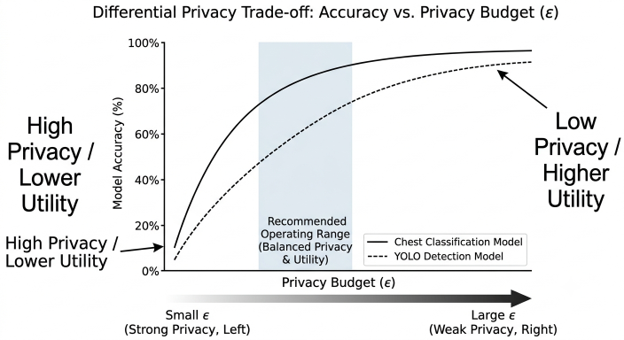
\includegraphics[width=0.8\textwidth]{assets/privacy_utility_tradeoff.png}
	\caption{Privacy--utility tradeoff under $(\epsilon,\delta)$-differential privacy. Smaller values of $\epsilon$ provide stronger privacy guarantees but may reduce model performance.}
	\label{fig:dp_tradeoff}
\end{figure}

\subsubsection{Additional Privacy Considerations}

Beyond gradient inversion attacks, model inversion and membership inference attacks represent additional privacy concerns.

Model inversion attempts to reconstruct representative training samples from a trained model, while membership inference seeks to determine whether a specific record was used during training.

Federated aggregation, large batch sizes, and differential privacy collectively reduce the effectiveness of these attack vectors.

\subsubsection{Transport-Layer Security (TLS)}

All model parameter exchanges are protected using mutual Transport Layer Security (mTLS) over gRPC.

The security infrastructure consists of:

\begin{itemize}
	\item Certificate Authority certificate (\texttt{ca.crt})
	\item Server certificate (\texttt{server.pem})
	\item Server private key (\texttt{server.key})
\end{itemize}

Mutual authentication ensures confidentiality, integrity, server authentication, and client authentication during communication.

In production deployments, TLS is mandatory and protects all federated learning traffic against interception and tampering.

\subsubsection{Authentication and Access Control}

Each participating institution receives a unique client identifier and API key during enrollment.

These credentials are required before client startup and are validated for every REST API request.

The authentication framework ensures:

\begin{itemize}
	\item Only authorized hospitals can participate.
	\item Unauthorized clients cannot submit updates.
	\item Client activity can be audited through server logs.
	\item Credentials remain external to source code repositories.
\end{itemize}

\subsubsection{Round Integrity and Liveness Controls}

The system continuously verifies round status before and during local training.

If a round is cancelled or completed, participating clients immediately terminate local computation and prevent obsolete updates from reaching the aggregation server.

Heartbeat messages are transmitted every fifteen seconds, enabling real-time monitoring of client availability and participation status.

These mechanisms improve both system integrity and operational reliability.

\subsubsection{Security Implementation Status Summary}

Table~\ref{tab:security_controls} summarizes the implementation status of all security controls incorporated into the federated learning platform.

\begin{table}[H]
	\centering
	\caption{Security Controls -- Implementation Status}
	\label{tab:security_controls}
	\renewcommand{\arraystretch}{1.2}
	\begin{tabularx}{\textwidth}{|p{3.8cm}|p{2cm}|p{1.8cm}|X|}
		\hline
		\textbf{Security Control} &
		\textbf{Category} &
		\textbf{Status} &
		\textbf{Notes} \\
		\hline
		
		Data locality (no raw data transmitted) &
		Privacy &
		Done &
		Core FL design property; only weight tensors transmitted \\
		\hline
		
		TLS encryption on gRPC channel &
		Transport &
		Done &
		\texttt{ca.crt} + \texttt{server.pem} + \texttt{server.key}; mutual TLS \\
		\hline
		
		API key authentication &
		Access Control &
		Done &
		\texttt{CLIENT\_API\_KEY} required; validated on every REST call \\
		\hline
		
		Client identity validation &
		Access Control &
		Done &
		\texttt{CLIENT\_ID} required; startup exit if absent \\
		\hline
		
		Large batch size ($B \geq 32$) &
		Privacy &
		Done &
		Mitigates gradient inversion attack fidelity \\
		\hline
		
		Heartbeat liveness monitoring &
		Integrity &
		Done &
		Continuous per-client liveness signal every 15 seconds \\
		\hline
		
		Per-epoch round-active check &
		Integrity &
		Done &
		Aborts training on cancelled round; covers both model types \\
		\hline
		
		Best-model checkpoint (local) &
		Robustness &
		Done &
		Restores best validation-loss weights before uploading to server \\
		\hline
		
		Selective YOLO federation (no head) &
		Integrity &
		Done &
		\texttt{cv3} detection head excluded from aggregation to prevent shape mismatch \\
		\hline
		
		Differential Privacy (DP noise) &
		Privacy &
		CONFIG-URABLE &
		Architecture supports $(\epsilon,\delta)$-DP; not yet enabled by default \\
		\hline
		
		Secure credential storage &
		Access Control &
		Done &
		\texttt{.env.template} pattern; credentials never stored in source code or container images \\
		\hline
		
		Shutdown-on-breach notification &
		Resilience &
		Done &
		Server sends \texttt{round-failed} webhook on unexpected shutdown \\
		\hline
		
	\end{tabularx}
\end{table}

The current implementation includes fully operational transport security, authentication, access control, liveness monitoring, and round integrity mechanisms. Differential privacy remains available as a configurable enhancement for deployments requiring stronger formal privacy guarantees.
\subsection{What Makes the Proposed System Distinctive}
\label{subsec:fl_novelty}
 
While federated learning has been applied in various medical imaging studies,
the majority of existing implementations are designed around a fixed model
architecture and a specific anatomical target, limiting their transferability
to new clinical tasks. The proposed framework differentiates itself through
the following design principles:
 
\textbf{Model Agnosticism.} The federated coordination layer — encompassing
client management, weight serialization, aggregation, and communication — is
fully decoupled from the local model definition. Any differentiable model
that can be expressed as a parameter vector (e.g., CNNs for classification,
U-Net variants for segmentation, Vision Transformers) can be substituted as
the local model without modifying the federated infrastructure. This makes
the system immediately applicable to new imaging tasks simply by swapping the
model definition on the client side.
  
\textbf{Staged Data Integration.} The system incorporates a staged data
feeding protocol that progressively increases each client's active training
subset across federated rounds. This design reflects the clinical reality
that expert-annotated medical imaging datasets grow incrementally over time
as radiologists label new cases. Rather than requiring a fully annotated
dataset before training begins, the system accommodates continuous data
growth, enabling earlier model deployment and iterative improvement as
annotation progresses.
 
\textbf{Containerized Reproducibility.} Each participating node is deployed
as an isolated Docker container, ensuring that the federated environment is
fully reproducible across different hardware configurations and operating
systems. The container-based architecture also simplifies scaling: adding a
new institution requires only the deployment of an additional client
container with the appropriate data volume mount, with no changes to the
server or existing clients.
 
\textbf{Framework Choice.} The system is implemented using the Flower
(flwr) framework~\cite{beutel2022}, selected for its support of multiple
ML backends (PyTorch, TensorFlow, JAX), its clean abstraction of the
client-server protocol, and its active development for healthcare FL
research. The backend-agnostic design of Flower further reinforces the
model-agnostic objective of the proposed system.
 
Collectively, these properties position the proposed FL framework as a
general-purpose infrastructure for privacy-preserving collaborative medical
image analysis, extensible to a wide range of clinical specialties and
diagnostic tasks without architectural redesign.


\section{Retrieval-Augmented Generation (RAG) Model}

The proposed platform incorporates a Retrieval-Augmented Generation (RAG) model to provide an intelligent medical question-answering assistant capable of responding to user inquiries using trusted medical knowledge sources. Unlike conventional large language models that rely solely on their internal parametric knowledge, the RAG approach augments the language model with information retrieved from an external knowledge base at inference time. This enables the system to generate responses that are more accurate, context-aware, explainable, and grounded in domain-specific medical information.

The primary objective of integrating the RAG model within the proposed framework is to provide users with a reliable conversational assistant capable of answering questions related to chest diseases, lung cancer, medical imaging, diagnostic procedures, and other healthcare-related topics. By retrieving relevant information from curated medical documents before response generation, the system significantly reduces hallucinations and improves the factual consistency of generated answers.

\subsection{Motivation}

Although modern Large Language Models (LLMs) demonstrate remarkable natural language understanding and generation capabilities, they suffer from several limitations when deployed in healthcare environments. Most notably, they may generate inaccurate information, provide outdated medical recommendations, or produce responses unsupported by clinical evidence.

In medical applications, such limitations can negatively affect user trust and potentially lead to harmful outcomes. Consequently, relying solely on the internal knowledge of a pretrained language model is insufficient for healthcare-oriented systems.

Retrieval-Augmented Generation addresses these challenges by combining information retrieval techniques with generative language models. Instead of answering questions exclusively from learned parameters, the system first retrieves relevant medical knowledge from an external document repository and then uses this information to guide response generation. This approach ensures that answers remain grounded in verified sources while maintaining the conversational capabilities of modern language models.

\subsection{Overview of the Proposed RAG Architecture}

The implemented RAG system consists of four major components:

\begin{enumerate}
	\item Medical Knowledge Base
	\item FAISS Vector Database
	\item Ollama Large Language Model
	\item LangChain Orchestration Layer
\end{enumerate}

The interaction between these components is illustrated in Figure~\ref{fig:rag_architecture}.

\begin{figure}[htbp]
	\centering
	
	\resizebox{\linewidth}{!}{
		\begin{tabular}{c c c c c c c c c}
			
			\fbox{
				\begin{tabular}{c}
					User\\
					Query
				\end{tabular}
			}
			
			&
			$\rightarrow$
			&
			
			\fbox{
				\begin{tabular}{c}
					Query\\
					Processing
				\end{tabular}
			}
			
			&
			$\rightarrow$
			&
			
			\fbox{
				\begin{tabular}{c}
					Embedding\\
					Generation
				\end{tabular}
			}
			
			&
			$\rightarrow$
			&
			
			\fbox{
				\begin{tabular}{c}
					FAISS\\
					Vector Search
				\end{tabular}
			}
			
			&
			$\rightarrow$
			&
			
			\fbox{
				\begin{tabular}{c}
					Relevant\\
					Document Chunks
				\end{tabular}
			}
			
		\end{tabular}
	}
	
	\vspace{0.6cm}
	
	$\downarrow$
	
	\vspace{0.4cm}
	
	\resizebox{0.8\linewidth}{!}{
		\begin{tabular}{c c c c c}
			
			\fbox{
				\begin{tabular}{c}
					Context\\
					Construction
				\end{tabular}
			}
			
			&
			$\rightarrow$
			&
			
			\fbox{
				\begin{tabular}{c}
					Qwen 2.5\\
					(LLM)
				\end{tabular}
			}
			
			&
			$\rightarrow$
			&
			
			\fbox{
				\begin{tabular}{c}
					Response\\
					Generation
				\end{tabular}
			}
			
		\end{tabular}
	}
	
	\vspace{0.6cm}
	
	$\downarrow$
	
	\vspace{0.4cm}
	
	\fbox{
		\begin{minipage}{0.45\linewidth}
			\centering
			Final Response + Source References
		\end{minipage}
	}
	
	\caption{Overall architecture of the proposed Retrieval-Augmented Generation (RAG) model. The user query is transformed into vector embeddings, relevant medical knowledge is retrieved from the FAISS vector database, and the retrieved context is supplied to the Qwen 2.5 language model to generate a grounded and source-aware response.}
	\label{fig:rag_architecture}
\end{figure}

The architecture begins when a user submits a natural language query through the platform interface. The query is forwarded to the FastAPI model backend, where LangChain orchestrates the retrieval and generation pipeline. Relevant document chunks are retrieved from the FAISS vector database and supplied as contextual information to the language model. The generated answer is then returned to the user along with references to the retrieved sources.

\subsection{Knowledge Base Construction}

The foundation of the RAG system is a curated collection of medical documents covering topics related to:

\begin{itemize}
	\item Chest diseases
	\item Pneumonia
	\item Tuberculosis
	\item COVID-19
	\item Lung cancer
	\item Medical imaging
	\item Diagnostic procedures
	\item Healthcare guidelines
\end{itemize}

These documents are converted into machine-processable representations before being indexed. Since language models cannot efficiently search through large collections of raw documents during inference, each document is divided into smaller semantic chunks.

Chunking improves retrieval accuracy by allowing the system to retrieve only the most relevant portions of a document rather than entire files.

For each generated chunk, metadata is preserved, including:

\begin{itemize}
	\item Document name
	\item Page number
	\item Source identifier
	\item Document category
\end{itemize}

This metadata later enables source attribution and transparency within generated responses.

\subsection{Vector Embedding Generation}

After document chunking, each text segment is transformed into a dense numerical representation known as an embedding vector.

Embeddings encode semantic meaning into a high-dimensional vector space, allowing documents with similar meanings to be located near one another mathematically.

Given a document chunk $(d\_i)$, an embedding function (E($\cdot$)) produces a vector representation $v_i = E(d_i)$ 
where $v_i \in \mathbb{R}^{n}$ and $(n)$ represents the embedding dimensionality.

These embeddings capture semantic relationships between medical concepts and enable similarity-based retrieval during inference.

\subsection{FAISS Vector Database}

To support efficient retrieval over thousands of embedded document chunks, the system employs Facebook AI Similarity Search (FAISS).

FAISS is a high-performance vector database specifically designed for similarity search within large embedding collections. Instead of performing keyword matching, FAISS retrieves documents based on semantic similarity.

All generated embeddings are stored within the FAISS index.

During inference, a user query is embedded using the same embedding model: $q = E(x)$ where $(x)$ denotes the user's query.

The FAISS index then searches for the (k) nearest vectors according to cosine similarity and returns the most relevant document chunks.

This retrieval process allows the system to locate contextually relevant medical information even when the exact wording differs from that found in the original documents.

\subsection{Large Language Model Integration}

The generative component of the RAG pipeline utilizes the Qwen 2.5 language model deployed locally through Ollama.

Running the model locally provides several advantages:

\begin{itemize}
	\item Reduced operational cost
	\item Improved privacy
	\item Low latency
	\item Full deployment control
	\item Offline inference capability
\end{itemize}

The model configuration used in the implementation is summarized in Table~\ref{tab:rag_model_configuration}.

\begin{table}[htbp]
	\centering
	\caption{Configuration of the deployed language model.}
	\label{tab:rag_model_configuration}
	\begin{tabular}{|l|l|}
		\hline
		\textbf{Parameter} & \textbf{Value} \\ 
		\hline
		LLM Engine & Ollama \\
		\hline
		Model & qwen2.5:3b \\
		\hline
		Temperature & 0.5 \\
		\hline
		Max Tokens & 500 \\
		\hline
		Keep Alive & Infinite (-1) \\
		\hline
	\end{tabular}
\end{table}

After retrieval, the selected document chunks are appended to the prompt supplied to the language model. Consequently, generated responses become grounded in retrieved medical knowledge rather than relying exclusively on pretrained parameters.

\subsection{Query Processing Workflow}

The complete RAG workflow implemented within the system is illustrated in Figure~\ref{fig:rag_workflow}.

\begin{figure}[htbp]
	\centering
	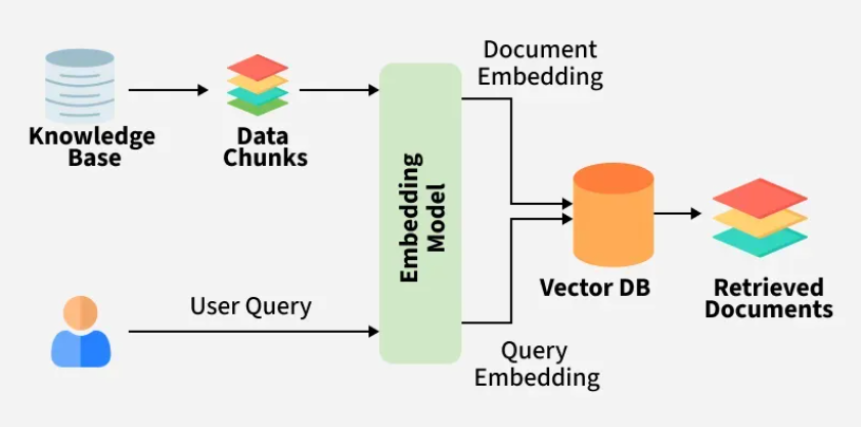
\includegraphics[width=\linewidth]{assets/RAG_1.png}
	\caption{Query processing workflow of the proposed RAG system.}
	\label{fig:rag_workflow}
\end{figure}

The workflow consists of the following steps:

\begin{enumerate}
	\item User submits a medical question.
	\item Query is forwarded to the FastAPI backend.
	\item Query embedding is generated.
	\item FAISS retrieves the most relevant document chunks.
	\item Retrieved context is assembled.
	\item Context and user query are passed to Qwen 2.5.
	\item The language model generates a grounded response.
	\item Source metadata is attached.
	\item Final response is returned to the user.
\end{enumerate}

\subsection{Source Attribution and Explainability}

One of the most important characteristics of the proposed RAG implementation is transparency.

Rather than generating answers without justification, the system preserves metadata associated with retrieved documents and returns source references alongside generated responses. This allows users to trace the origin of information and verify the supporting evidence used during answer generation. The underlying report emphasizes that retrieved documents and page references are preserved to improve transparency and user trust.

Providing source-aware responses is particularly important in healthcare applications where explainability and evidence-based recommendations are essential.

\subsection{Advantages of the Proposed Approach}

The implemented Retrieval-Augmented Generation model provides several advantages:

\begin{itemize}
	\item Reduces hallucinations compared with standalone LLMs.
	\item Produces responses grounded in medical knowledge sources.
	\item Supports explainable and source-aware answers.
	\item Enables efficient retrieval through FAISS vector search.
	\item Preserves privacy through local deployment using Ollama.
	\item Can be continuously expanded by adding new medical documents.
	\item Integrates seamlessly with the overall X-Fed Neuroscan architecture.
\end{itemize}

Consequently, the RAG subsystem serves as an intelligent medical assistant that complements the image analysis capabilities of the platform by providing users with reliable, contextualized, and explainable healthcare information.


\section{Platform Architecture}
The system  is a comprehensive web-based healthcare management system developed to streamline medical services and enhance diagnostic workflows through an integrated digital platform. The system provides a centralized environment where patients, doctors, administrators, and healthcare institutions can interact efficiently through role-based dashboards and specialized services.
The platform allows patients to create accounts, manage their profiles, book appointments, track medical records, and communicate through an intelligent healthcare assistant. Doctors can manage appointments, analyze medical images, review patient information, and assign diagnostic results, while administrators oversee user management, system operations, and hospital coordination. The system also supports healthcare institutions participating in collaborative AI model development through federated learning mechanisms.
Built using a modern multi-tier architecture, XFed NeuroScan combines a responsive web interface, secure backend services, cloud-based storage, and artificial intelligence modules to deliver a seamless user experience. The application emphasizes security, scalability, and usability by implementing role-based access control, secure authentication, real-time communication, and centralized healthcare workflows.
By integrating healthcare management features with intelligent diagnostic services, XFed NeuroScan provides a unified platform that improves operational efficiency, supports medical decision-making, and enhances the overall experience for both healthcare providers and patients.

The platform is composed of four tightly integrated repositories:
\begin{itemize}
	\item \textbf{Frontend:} React 18 single-pages application serving doctors, patients, and administrators.
	\item \textbf{Backend:} Spring Boot 3.5 REST and WebSocket API acting as the central system of record, handling authentication, business logic, user management, and communication between services.
	\item \textbf{Model Backend:} FastAPI-based AI service responsible for medical image analysis, chest disease classification, lung cancer detection, explainable AI heatmap generation, and a Retrieval-Augmented Generation (RAG) medical chatbot for intelligent question answering.
	\item \textbf{Federated-Learning Server:} Flower-based federated learning coordinator managing hospital registration, client monitoring, distributed training rounds, and global model aggregation.
\end{itemize} 
Together, these components provide a complete healthcare platform that combines medical workflow management, AI-assisted diagnosis, intelligent medical assistance through RAG, and privacy-preserving federated learning across multiple healthcare institutions.

\begin{table}[htbp]
	\centering
	\caption{Summary of the proposed X-Fed NeuroScan framework.}
	\label{tab:framework_summary}
	\begin{tabular}{|p{4cm}|p{9cm}|}
		\hline
		\textbf{Dimension} & \textbf{Detail} \\
		\hline
		Primary Domain & Medical imaging and AI-based diagnostic systems \\
		\hline
		Key Innovation & Federated learning for privacy-preserving model improvement and collaborative model training across institutions \\
		\hline
		User Roles & Patient, Doctor, and Administrator \\
		\hline
		Imaging Modalities & Chest X-ray classification (COVID-19, Tuberculosis, Pneumonia, and Normal) and lung cancer detection from CT scans \\
		\hline
		AI Explainability & Grad-CAM heatmaps for chest disease predictions and lesion localization visualizations for lung cancer detection \\
		\hline
		Privacy Model & Raw medical images never leave hospital premises; only model parameters are exchanged during federated learning \\
		\hline
	\end{tabular}
\end{table}

\subsection{End-to-End System Architecture}The system follows a microservices architecture. Four independent services communicate over well-defined APIs. The frontend is the only entry point for human users; all backend services are internal.

\subsubsection{Service Map}
Table~\ref{tab:system_components} lists all the different components and services of the proposed system.
\begin{table}[htbp]
	\centering
	\caption{Technological components of the proposed system architecture.}
	\label{tab:system_components}
	\begin{tabular}{|p{3.5cm}|p{4.5cm}|p{2cm}|p{5cm}|}
		\hline
		\textbf{Service} & \textbf{Technology} & \textbf{Port} & \textbf{Primary Role} \\
		\hline
		Frontend &
		React 18, Vite, and TypeScript &
		3000 &
		User interface for patients, doctors, and administrators \\
		\hline
		
		Backend &
		Spring Boot 3.5 and Java 21 &
		8080 &
		Authentication, business logic implementation, and API gateway services \\
		\hline
		
		Model Backend &
		FastAPI and Python 3 &
		8000 &
		Machine learning inference services and retrieval-augmented generation (RAG) chatbot functionality \\
		\hline
		
		Federated Learning Server &
		FastAPI, Flower, and Python 3 &
		8001 / 50051 &
		Federated learning coordination, client management, and hospital registry services \\
		\hline
	\end{tabular}
\end{table}

\subsubsection{External Infrastructure}
During system implementation, we  have also relied on external components to not reinvent the wheel  and leverage already existing powerful and free infrastructure, those components are listed in Table~\ref{tab:supporting_infrastructure}
\begin{table}[htbp]
	\centering
	\caption{Supporting infrastructure and external services used by the proposed system.}
	\label{tab:supporting_infrastructure}
	\begin{tabular}{|p{4.5cm}|p{10cm}|}
		\hline
		\textbf{Component} & \textbf{Role} \\
		\hline
		
		Cloudflare R2 (S3-Compatible Storage) &
		Stores uploaded medical images, generated Grad-CAM heatmaps, lung cancer detection result overlays, and other imaging-related artifacts. \\
		\hline
		
		PostgreSQL &
		Primary relational database used to manage users, medical images, appointments, hospital information, federated learning participants, and other persistent application data. \\
		\hline
		
		Redis &
		Provides high-speed storage for refresh tokens and caching of presigned URLs to improve system performance and reduce unnecessary storage requests. \\
		\hline
		
		Ollama (qwen2.5:3b) &
		Local large language model (LLM) responsible for generating responses within the retrieval-augmented generation (RAG) chatbot component. \\
		\hline
		
		Gmail SMTP &
		Handles transactional email services including password reset requests, user invitations, account notifications, and hospital package communications. \\
		\hline
		
		FAISS &
		Vector similarity search engine used to index and retrieve relevant documents for the retrieval-augmented generation (RAG) pipeline. \\
		\hline
		
	\end{tabular}
\end{table}

\subsubsection{Architecture Visualization}

To provide a clearer understanding of the overall system structure, Figures~\ref{fig:system_architecture_overview} and \ref{fig:deployment_architecture_overview} present visual representations of the proposed \textit{X-Fed NeuroScan} framework. These diagrams complement the architectural descriptions presented throughout this chapter by illustrating the interaction between system components, data flow pathways, and deployment services. Together, they provide a comprehensive view of both the logical architecture of the framework and the technological infrastructure used to support its operation.

\begin{figure}[htbp]
	\centering
	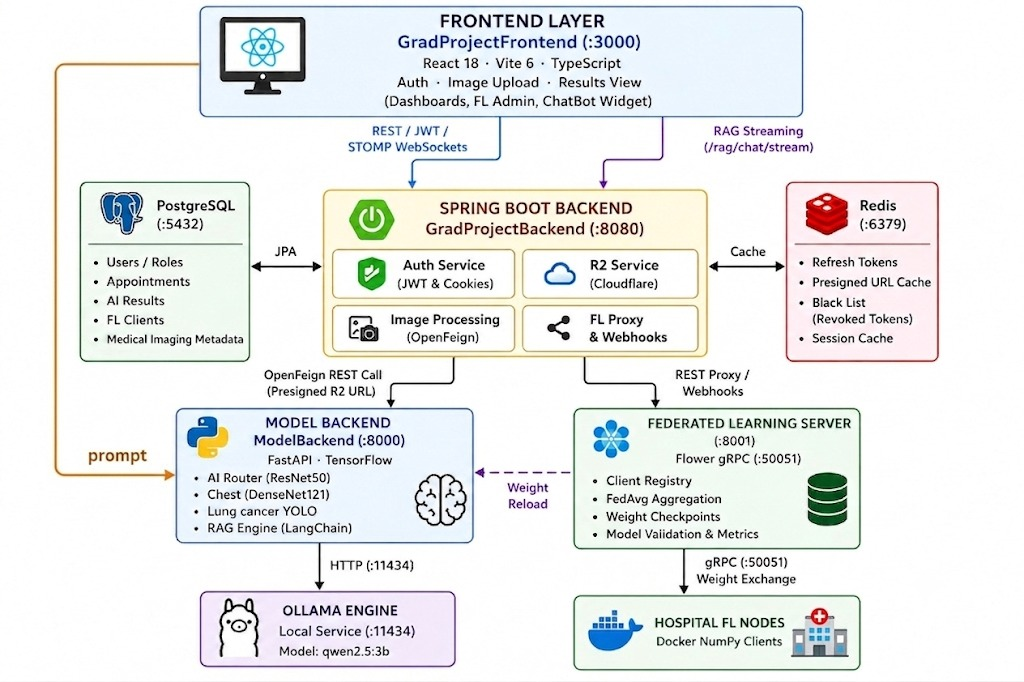
\includegraphics[width=0.95\linewidth]{assets/backend-1-ag.jpeg}
	\caption{End-to-end logical architecture of the proposed X-Fed NeuroScan framework, illustrating the interaction between users, backend services, AI models, explainability components, federated learning infrastructure, and data storage systems.}
	\label{fig:system_architecture_overview}
\end{figure}

\begin{figure}[htbp]
	\centering
	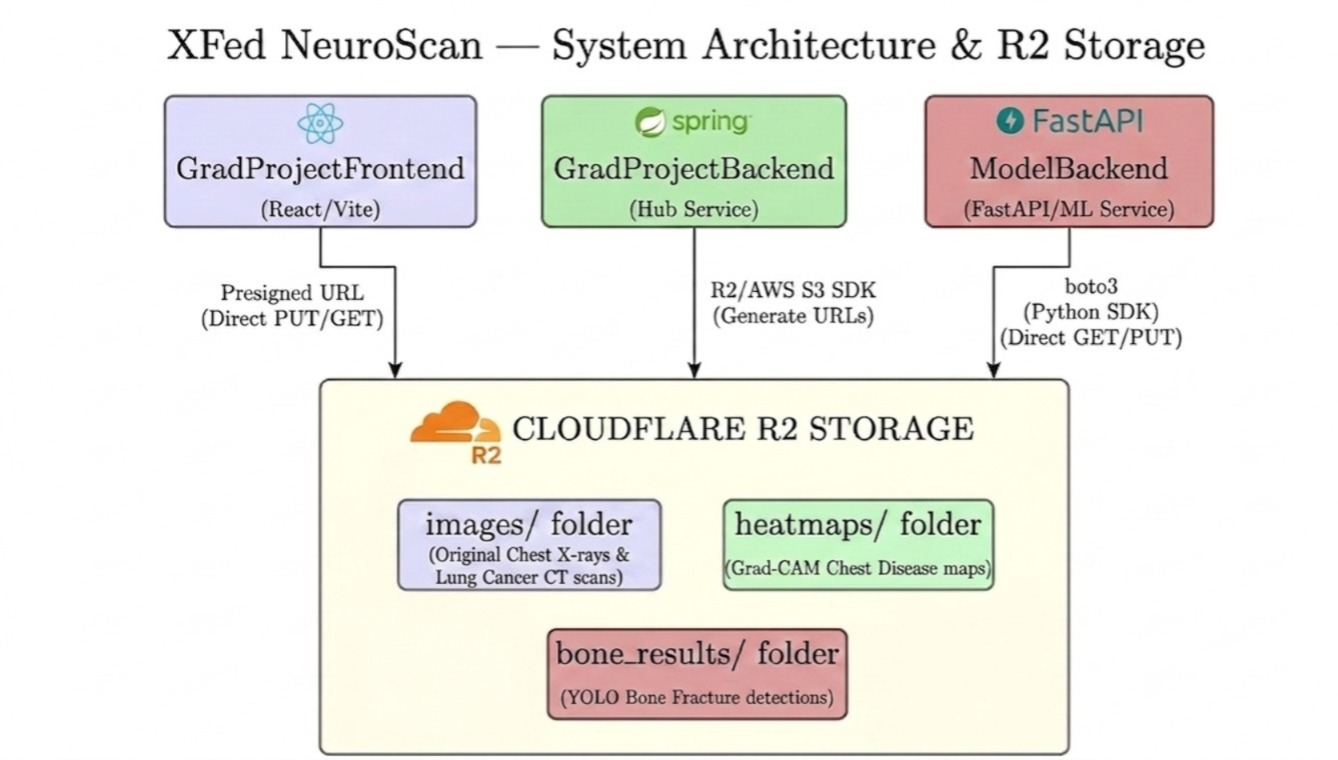
\includegraphics[width=0.95\linewidth]{assets/backend-2-ag.jpeg}
	\caption{Deployment architecture of the proposed system showing the frontend application, backend services, model-serving infrastructure, federated learning server, databases, storage components, and external integrations.}
	\label{fig:deployment_architecture_overview}
\end{figure}

\subsection{Frontend}
The frontend is a React 18 single-page application built with Vite 6 and TypeScript. It serves three user roles — Patient, Doctor, and Admin — through role-gated dashboards, and is the sole human interface into the platform.

\subsubsection{Technology Stack}
Different technologies were used during the development and implementation of the frontend components of the proposed system. They have been listed in Table~\ref{tab:frontend_technologies}.
\begin{table}[htbp]
	\centering
	\caption{Frontend technologies used in the implementation of the proposed system.}
	\label{tab:frontend_technologies}
	\begin{tabular}{|p{4cm}|p{8.5cm}|}
		\hline
		\textbf{Category} & \textbf{Technology} \\
		\hline
		
		Framework &
		React 18 \\
		\hline
		
		Build Tool &
		Vite 6 with \texttt{@vitejs/plugin-react-swc} \\
		\hline
		
		Programming Language &
		TypeScript 5 (Strict Mode) \\
		\hline
		
		Routing &
		React Router 7 \\
		\hline
		
		Styling &
		Tailwind CSS v4 \\
		\hline
		
		UI Primitives &
		Radix UI with shadcn-style wrapper components \\
		\hline
		
		Animations &
		Framer Motion (Motion) \\
		\hline
		
		Charts and Data Visualization &
		Recharts \\
		\hline
		
		Real-Time Communication &
		\texttt{@stomp/stompjs} and \texttt{sockjs-client} \\
		\hline
		
		Form Management &
		react-hook-form \\
		\hline
		
	\end{tabular}
\end{table}

\subsubsection{User Roles \& Capabilities}
The system is designed as a role-based healthcare to ensure that each type of user interacts with the platform according to their responsibilities, permissions, and level of access. The system defines three main roles: Patient, Doctor, and Administrator, each serving a distinct purpose within the healthcare workflow.

Patients represent the end users of the system. Their role is limited to personal healthcare management, including registering accounts, booking appointments, viewing medical history, and accessing their own diagnostic results. This restricted access ensures that patients can interact with their healthcare data securely without modifying clinical or system-level information.

Doctors have a more advanced role focused on medical operations. They can upload and analyze medical images, review AI-generated predictions, interpret results, and assign diagnoses to patients. In addition, doctors manage appointments and clinical interactions with patients. This role requires broader access because it directly involves medical decision-making and the use of AI diagnostic tools.
Administrators hold the highest level of control within the system. They are responsible for managing users, including creating and inviting doctors, monitoring system activity, and overseeing hospital and federated learning operations. Administrators also handle system configuration and ensure that all services operate securely and efficiently.

The separation of roles is essential for maintaining security, privacy, and operational clarity. By limiting access based on responsibilities, the system prevents unauthorized actions, reduces the risk of data misuse, and ensures that each user interacts only with the features relevant to their function. This role-based design also improves usability by providing a tailored interface for each type of user, making the system more efficient and easier to navigate.

\begin{table}[htbp]
	\centering
	\caption{User roles and capabilities within the proposed X-Fed NeuroScan system.}
	\label{tab:user_roles_capabilities}
	\begin{tabular}{|p{3cm}|p{9.5cm}|}
		\hline
		\textbf{Role} & \textbf{Capabilities} \\
		\hline
		
		Patient &
		View personalized dashboard statistics, book appointments with doctors, upload medical image attachments, access diagnostic results, and review prediction history. \\
		\hline
		
		Doctor &
		Analyze chest medical images using the integrated AI models, assign diagnostic results to patients, manage appointment schedules, review patient records, and access prediction history. \\
		\hline
		
		Administrator &
		Perform full platform administration including user management, federated learning hospital registration, hospital selection for federated training rounds, monitoring system activity, and conducting image analysis through the integrated diagnostic framework. \\
		\hline
		
	\end{tabular}
\end{table}

\subsubsection{Key Pages and Routing}
Frontend is structured as a single-page application with role-based routing to ensure secure and organized access to system features. Each user type is directed to specific pages depending on their permissions and responsibilities within the platform.

Public users can access the landing page and authentication-related pages, including login, signup, password recovery, and invite-based account activation. These pages are only available to guests who are not yet authenticated.

Authenticated users are redirected to role-specific dashboards after login. Patients have access to their personal dashboard and medical history, where they can view appointments and diagnostic results. Doctors are provided with a dedicated dashboard along with access to image analysis tools and patient-related medical data. Administrators have the highest level of access, allowing them to manage users, monitor system activity, and control federated learning operations.

In addition to dashboards, administrators also access specialized modules for user management and federated learning configuration, including hospital registration and training round setup. The image analysis page is restricted to doctors and administrators due to its clinical importance and use of AI-based diagnostic tools.

Overall, the routing structure enforces strict role-based access control, ensuring that each user interacts only with the features relevant to their responsibilities while maintaining system security and usability.

\begin{table}[htbp]
	\centering
	\caption{Access control policy for system pages and administrative modules.}
	\label{tab:system_page_access_control}
	\begin{tabular}{|p{4cm}|p{6.5cm}|}
		\hline
		\textbf{Page} & \textbf{Access} \\
		\hline
		
		Landing Page &
		Publicly accessible to all users, including unauthenticated visitors. \\
		\hline
		
		Authentication Pages &
		Accessible only to guest users who have not yet authenticated. \\
		\hline
		
		Password Recovery &
		Accessible only to guest users initiating the password reset process. \\
		\hline
		
		Invite Activation &
		Accessible only through a valid invitation token provided to the invited user. \\
		\hline
		
		Image Analysis &
		Accessible to users with Administrator or Doctor privileges. \\
		\hline
		
		Prediction History &
		Accessible to Administrators, Doctors, and Patients according to their authorization level. \\
		\hline
		
		Administrator Dashboard &
		Accessible exclusively to users with the Administrator role. \\
		\hline
		
		Doctor Dashboard &
		Accessible exclusively to users with the Doctor role. \\
		\hline
		
		Patient Dashboard &
		Accessible exclusively to users with the Patient role. \\
		\hline
		
		User Management &
		Accessible exclusively to Administrators for managing user accounts and permissions. \\
		\hline
		
		Federated Learning Hospital Management &
		Accessible exclusively to Administrators for registering, updating, and monitoring participating hospitals. \\
		\hline
		
		Federated Learning Training Round Setup &
		Accessible exclusively to Administrators for configuring and launching federated learning training rounds. \\
		\hline
		
	\end{tabular}
\end{table}

\subsubsection{Core Features}
\paragraph{Authentication \& Session Management}
The frontend implements a full authentication lifecycle using JWT access tokens are stored in memory (not localStorage); refresh tokens are stored in HttpOnly cookies. On app load, the context attempts a silent token refresh to restore sessions without requiring re-login. GuestRoute prevents authenticated users from visiting auth. pages; Require Dashboard Role guards all dashboard routes.

\paragraph{Medical Image Analysis}
The image analysis flow uses a presigned-URL pattern to avoid routing large files through the backend:
\begin{itemize}
	\item Step 1: Frontend requests a presigned R2 PUT URL from Spring Backend 
	\item Step 2: Frontend uploads the image directly to Cloudflare R2
	\item Step 3: Frontend calls the api who is responsible for image-processing with the R2 key
	\item Step 4: Backend triggers Model inference and returns prediction, confidence, and heatmap URL
\end{itemize}

\paragraph{Federated Learning Management}
Admins manage FL hospitals through two dedicated pages. FLHospitalsPage shows all registered hospital nodes with live ONLINE/OFFLINE status via WebSocket. FL Select Hospitals Page lets admins choose which hospitals participate in the next training round. Registration generates an API key displayed once via ApiKeySuccessDialog.

\paragraph{AI Chatbot (RAG)}
A floating chat widget  is available on every page. Responses are streamed from the RAG service. The chatbot gracefully degrades to keyword-based mock answers if the RAG API is unreachable.

\begin{figure}[htbp]
	\centering
	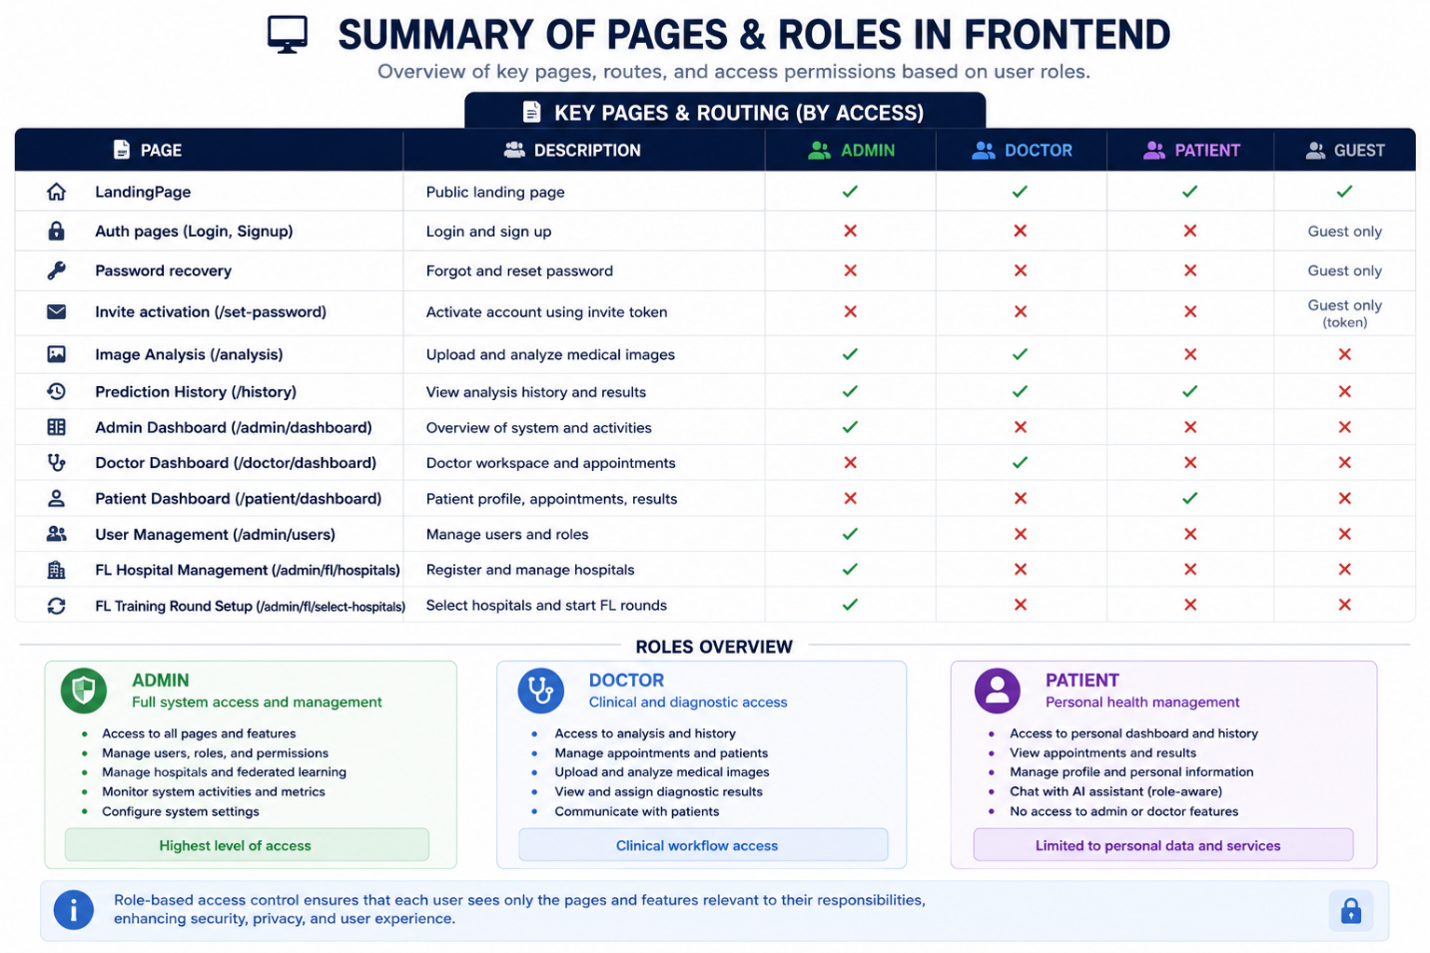
\includegraphics[width=0.95\linewidth]{assets/backend3.png}
	\caption{A visualization of the roles and pages implemented in the web application.}
	\label{fig:roles_pages_summary}
\end{figure}

\subsection{Centralized Backend (Spring Boot)}
Centralized backend is a Spring Boot 3.5 application written in Java 21. It serves as the central API gateway and system of record for authentication, user management, medical image orchestration, appointments, federated learning coordination, and real-time WebSocket broadcasts. 

\subsubsection{Technology Stack}
Various technologies were utilized in the implementation of the backend of the proposed end-to-end system. All of these technologies are listed in Table~\ref{tab:backend_technologies}.
\begin{table}[htbp]
	\centering
	\caption{Backend technologies used in the implementation of the proposed system.}
	\label{tab:backend_technologies}
	\begin{tabular}{|p{4cm}|p{8.5cm}|}
		\hline
		\textbf{Category} & \textbf{Technology} \\
		\hline
		
		Framework &
		Spring Boot 3.5.4 \\
		\hline
		
		Programming Language &
		Java 21 \\
		\hline
		
		Build Tool &
		Maven \\
		\hline
		
		Security &
		Spring Security 6 with JSON Web Token (JWT) authentication using JJWT 0.12.3 \\
		\hline
		
		Persistence Layer &
		Spring Data JPA, Hibernate, and PostgreSQL \\
		\hline
		
		Cache and Session Management &
		Spring Data Redis \\
		\hline
		
		HTTP Client &
		Spring Cloud OpenFeign \\
		\hline
		
		Real-Time Communication &
		Spring WebSocket, STOMP, and SockJS \\
		\hline
		
		Object Storage Integration &
		AWS SDK v2 for S3-compatible storage (Cloudflare R2) \\
		\hline
		
		Email Services &
		Spring Mail with Gmail SMTP \\
		\hline
		
		API Documentation &
		SpringDoc OpenAPI (Swagger UI) \\
		\hline
		
		Object Mapping and Code Generation &
		MapStruct and Lombok \\
		\hline
		
	\end{tabular}
\end{table}

\subsubsection{Security \& Authentication}

\begin{figure}[htbp]
	\centering
	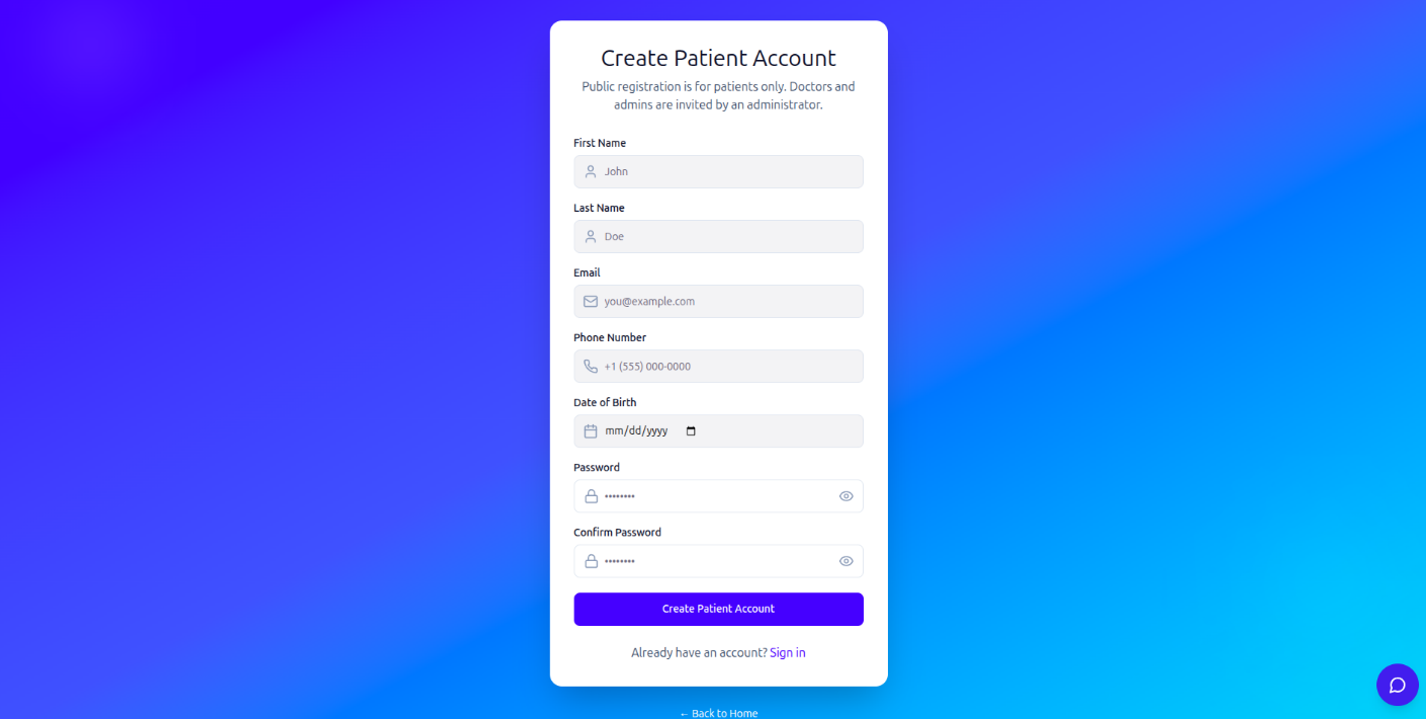
\includegraphics{assets/backend4.png}
	\caption{An image of the Create Account interaction from the web application.}
	\label{fig:create_account}
\end{figure}

\begin{figure}[htbp]
	\centering
	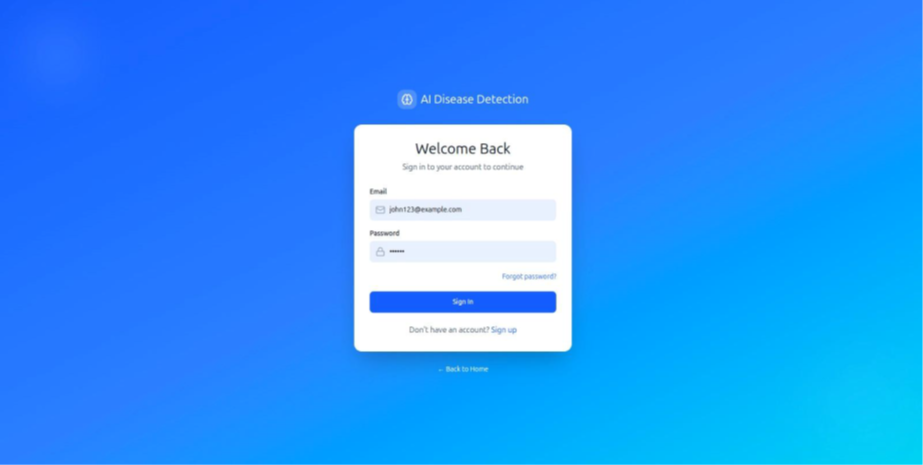
\includegraphics{assets/backend5.png}
	\caption{An image of the Login interaction from the web application.}
	\label{fig:login}
\end{figure}

Security is implemented with JWT access tokens and HttpOnly refresh-token cookies stored in Redis:
\begin{itemize}
	\item Access Tokens: short-lived JWTs returned in the login response body
	\item Refresh Tokens: longer-lived tokens stored in Redis (key: email:deviceId) and set as HttpOnly cookies
	\item Logout: access tokens blacklisted when still valid; refresh token deleted from Redis
	\item FL API keys: encrypted at rest using AES via EncryptionUtils
	\item FL webhook endpoints: authenticated with a shared secret (not JWT)
	\item Soft delete: deleted users cannot log in
\end{itemize}

In the current system design, \textbf{login is restricted to patients only}. Doctor and Admin accounts are not self-authenticated through public signup; instead, they are created and managed exclusively by an administrator and activated through an invitation-based workflow. This ensures strict control over privileged roles in the healthcare system.

After login, user information is stored in PostgreSQL, but sensitive session data is handled separately for security. Passwords are never stored in plain text; instead, they are hashed using \textbf{BCrypt} before being saved in the database, making them irreversible and protected even if the database is compromised.

During authentication, the input password is hashed and compared with the stored hash. If valid, the system generates a short-lived \textbf{JWT access token} and a long-lived \textbf{refresh token}. The access token is used for API requests, while the refresh token is stored securely in \textbf{Redis} and also set as an \textbf{HttpOnly cookie}.

When the user logs out, the access token is blacklisted and the refresh token is removed from Redis, fully terminating the session. This design ensures secure password storage, stateless authentication, and strong session protection. 

In the system, only Admin users have the authority to create or manage Doctor and other Admin accounts, ensuring strict role control and preventing unauthorized privilege escalation.

New privileged users (Doctors or Admins) cannot register through the public signup process. Instead, an Admin must explicitly create or invite them through the administrative interface. This invitation-based flow allows the system to maintain tight control over sensitive roles that have access to clinical data, AI analysis tools, and system-wide management features.

\begin{figure}[htbp]
	\centering
	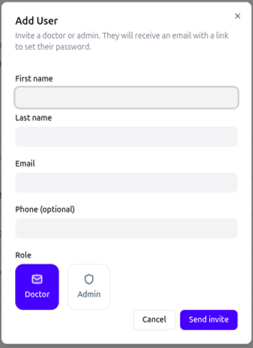
\includegraphics{assets/backend6.png}
	\caption{An image of the Add User interaction from the web application.}
	\label{fig:add_user}
\end{figure}

After an Admin creates a new Doctor or Admin account, the account does not become active immediately. Instead, it enters a pending state until it is explicitly approved. This approval step ensures that no privileged user gains access to the system without proper verification and administrative confirmation.

During this pending phase, the user record is already stored in the database, but the account remains inactive, meaning the user cannot log in or access any system features. Once the Admin approves the account, its status is updated to active, and the user is then able to authenticate and use the system according to their assigned role.

In the user management interface, the Admin has full control over viewing and organizing all system users through a role-based filtering system. This allows the Admin to efficiently manage large numbers of accounts by categorizing users according to their current role and status.

In addition to account creation and approval, the Admin also has full control over existing privileged accounts, as shown in \ref{fig:user_mgmt}. This includes the ability to disable or delete accounts at any time. Disabling an account temporarily prevents the user from logging in without removing their data, while deletion marks the account as removed (soft delete), ensuring it is excluded from authentication and system operations but still preserved for audit or historical purposes.

\begin{figure}[htbp]
	\centering
	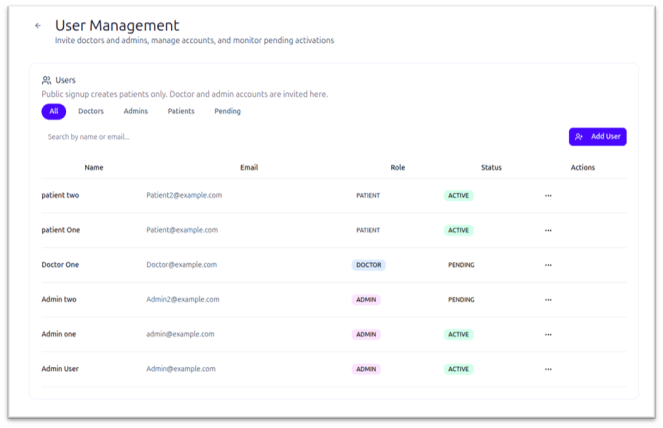
\includegraphics[width=0.95\linewidth]{assets/backend7.png}
	\caption{An image of the User Management tab from the web application.}
	\label{fig:user_mgmt}
\end{figure}

When a user selects “Forgot Password”, the system follows a secure multi-step flow to ensure that only the legitimate account owner can reset the password.

First, the user enters their registered email address in the frontend. This request is sent to the Spring Boot backend, which validates whether the email exists in the system. If the user is found, Spring Boot generates a secure password reset token, typically a short-lived, random token linked to the user account.

This token is then stored temporarily (or associated with the user record) and sent to the user via email using Gmail SMTP. The email contains a secure reset link that includes the token as a parameter.

When the user clicks the link, they are redirected to the password reset page in the frontend. The new password is submitted along with the token, and Spring Boot validates the token to ensure it is still valid and has not expired or been used before.

If the token is valid, the system hashes the new password using BCrypt and updates it in the PostgreSQL database, replacing the old password hash. After successful reset, the token is invalidated to prevent reuse.

Overall, the forgot password process ensures security by combining email verification, time-limited tokens, secure transmission, and encrypted password storage.

So in summary User authentication in system uses a secure JWT-based system where only patients can self-register and log in, while doctors and admins are created by admins. Passwords are stored in the database using BCrypt hashing.

After successful login, the system issues a short-lived JWT access token and a long-lived refresh token stored in Redis as an HttpOnly cookie. The access token is used for requests, and the refresh token allows session renewal.

The system also supports a secure forgot password workflow, where a password reset token is generated, sent to the user via email, and validated before allowing password updates. The new password is then hashed using BCrypt and stored in the database.

On logout, tokens are invalidated by blacklisting the access token and removing the refresh token. Role-based access control and soft delete ensure only authorized and active users can access the system.

\begin{figure}[htbp]
	\centering
	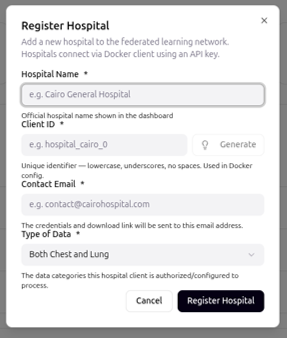
\includegraphics{assets/backend8.png}
	\caption{An image of the Add Hospital interaction from the web application.}
	\label{fig:add_hospital}
\end{figure}

\begin{figure}[htbp]
	\centering
	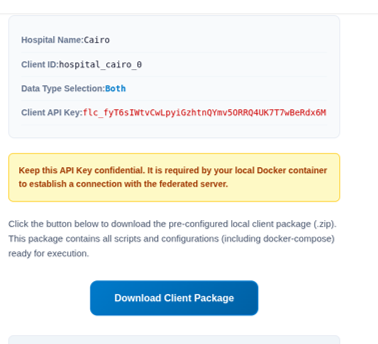
\includegraphics{assets/backend9.png}
	\caption{An image of the client hospital getting a confidential API key interaction from the web application.}
	\label{fig:hospital_api}
\end{figure}

Backend handles the full lifecycle of registering new hospitals in the federated learning system. When an Admin submits a hospital, Spring Boot validates the request, ensures only Admins can perform the action, and then generates a unique FL client ID and encrypted API key using AES before storing them in PostgreSQL. The hospital is initially saved with a PENDING or INACTIVE status.

After that, Spring Boot registers the hospital with the Federated Learning Server by sending its credentials and metadata, allowing it to join the federated learning network. It may also provide a Docker-based client package for hospital deployment.

Spring Boot receives and synchronizes key data from the Federated Learning (FL) Server, especially hospital online/offline status, which is determined by heartbeat signals sent from hospital clients to the FL Server. Spring Boot does not calculate this status itself; instead, it periodically fetches updated client information from the FL Server.

Overall, Spring Boot acts as a bridge that collects, stores, and distributes FL Server status updates, giving administrators a live view of the federated learning network.

When a new hospital is registered in the federated learning system, Spring Boot not only creates and stores the hospital record, but also sends an automated email notification via Gmail SMTP as part of the onboarding process.

After the Admin submits and approves the hospital registration, Spring Boot generates the hospital’s federated learning credentials (such as the FL client ID and encrypted API key) and securely stores them in the database. Once the registration is successfully completed, Spring Boot triggers the email service to notify the hospital.

This email is sent using Gmail SMTP integration and typically contains important onboarding information such as the hospital’s activation status, instructions for joining the federated learning network, and in some cases, a link or attachment for downloading the Docker-based FL client package required to connect to the FL server.

This step ensures that hospitals are immediately informed after registration and can proceed with setup and participation in federated learning without manual coordination. It also improves system automation and reduces administrative overhead while maintaining secure delivery of sensitive setup information.

\subsubsection{Medical Image Pipeline}
The backend orchestrates image analysis without storing raw images locally:
\begin{itemize}
	\item Presigned PUT URL is generated for direct R2 upload (5-minute expiry).
	\item After upload, backend saves image metadata to PostgreSQL
	\item ModelBackend is called via OpenFeign (Feign client) with a presigned GET URL
	\item ML results — prediction label, confidence score, heatmap S3 key — are persisted
	\item Presigned GET URLs for original and heatmap images are cached in Redis (~59 min TTL)
\end{itemize}

Small parts of the pipeline can be shown in \ref{fig:greeting_}, and \ref{fig:greeting_2} where the user is asked to upload a medical image to the system so that they are directed to the right models and diagnosed.

\begin{figure}[htbp]
	\centering
	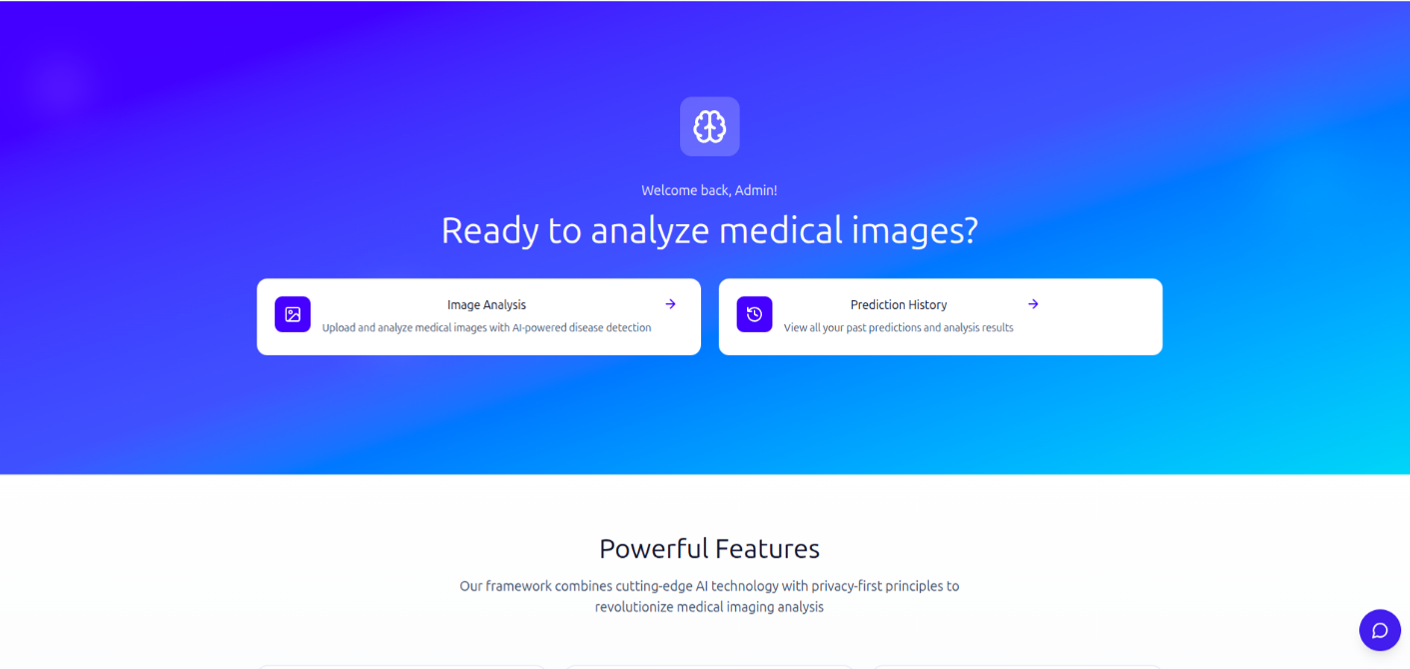
\includegraphics[width=0.95\linewidth]{assets/backend10.png}
	\caption{An image greeting page of the web application.}
	\label{fig:greeting_1}
\end{figure}

\begin{figure}[htbp]
	\centering
	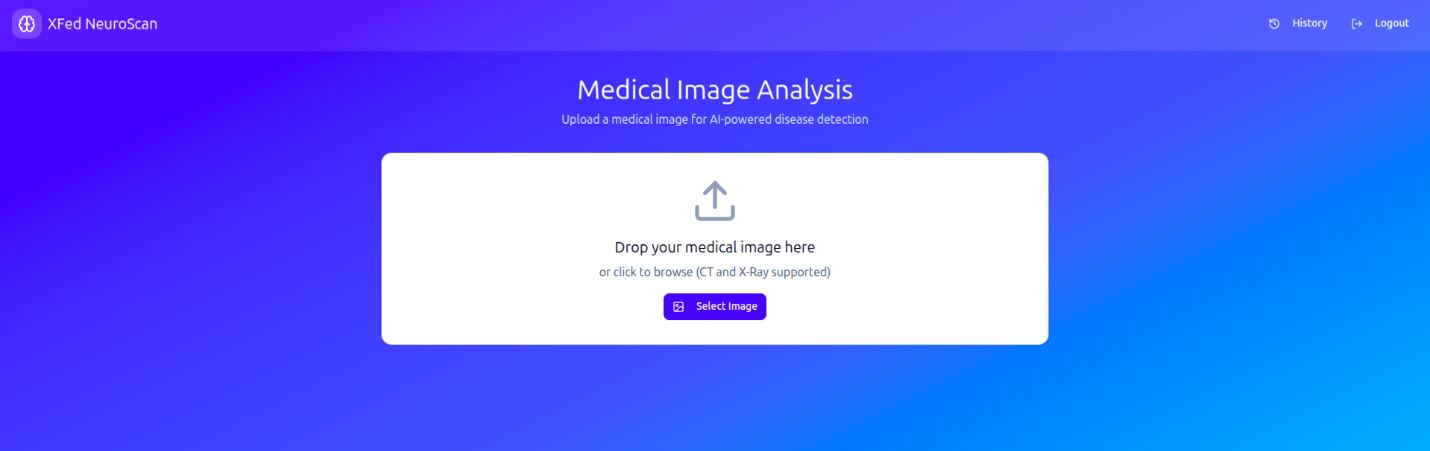
\includegraphics[width=0.95\linewidth]{assets/backend11.png}
	\caption{An image of the system asking the user to upload a scan to diagnose.}
	\label{fig:greeting_2}
\end{figure}

Prediction history can be viewed and also has statistics like (total scans , AVG. confidence) , and also every prediction’s details can be viewed or deleted, as shown in Figure~\ref{fig:pred_history}, and the details of each scan can be reviewed as well, as shown in Figure~\ref{fig:pred_review}.

\begin{figure}[htbp]
	\centering
	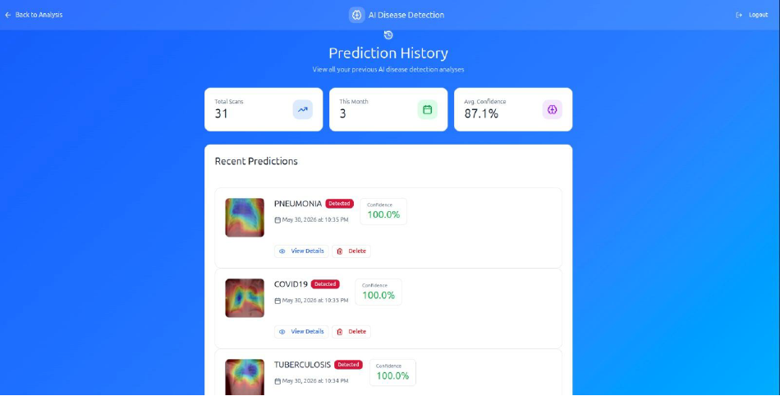
\includegraphics[width=0.95\linewidth]{assets/backend12.png}
	\caption{An image of the system showing the prediction history of the logged-in  user.}
	\label{fig:pred_history}
\end{figure}

\begin{figure}[htbp]
	\centering
	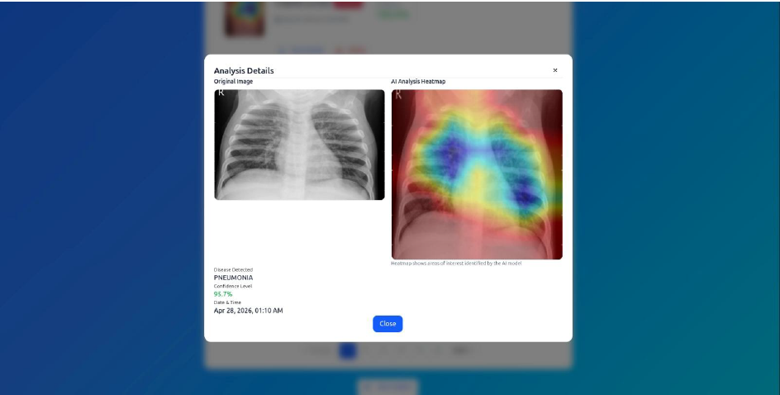
\includegraphics[width=0.95\linewidth]{assets/backend13.png}
	\caption{An image of the system showing the details of one of the user's historical predictions.}
	\label{fig:pred_review}
\end{figure}

Some examples of the Lung Cancer model in action are shown in Figure~\ref{fig:lung1}, and Figure~\ref{fig:lung2}. The system also makes sure to show the confidence as ordinary in medical applications of computer vision systems, as well as the processing time and the resulting heatmap, if applicable.

\begin{figure}[htbp]
	\centering
	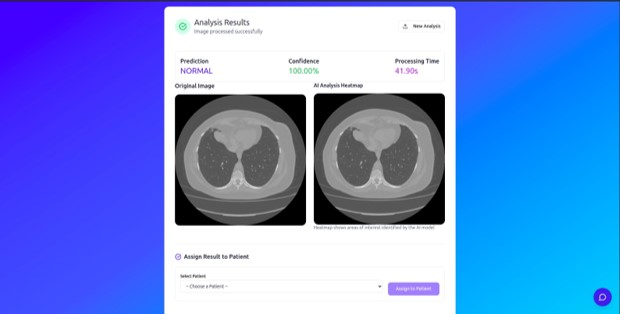
\includegraphics[width=0.95\linewidth]{assets/backend14.jpg}
	\caption{One of the of the examples of using the system on the a lung cancer image.}
	\label{fig:lung1}
\end{figure}

\begin{figure}[htbp]
	\centering
	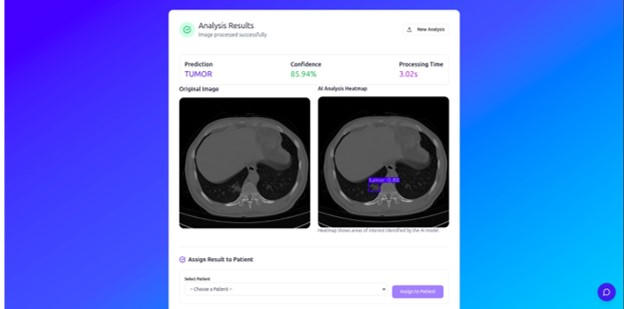
\includegraphics[width=0.95\linewidth]{assets/backend15.jpg}
	\caption{Another example of using the system on the a lung cancer image.}
	\label{fig:lung2}
\end{figure}

\subsubsection{Appointment Management}
The appointment management module enables patients and doctors to coordinate medical consultations through a structured workflow. Patients can create appointments by selecting a doctor, choosing a date and time, specifying the appointment type, and providing optional notes or supporting attachments. Once submitted, the appointment information is stored in the database and becomes available to the assigned doctor.

Doctors can view their scheduled appointments, review patient details, and update the appointment status as needed. They can mark appointments as completed, add consultation notes, or cancel appointments when necessary. Patients can also view the status of their appointments and track any updates made by the doctor.

All appointment data is managed through the Spring Boot backend and stored in PostgreSQL, ensuring persistence and secure access. The module provides an organized way to manage patient-doctor interactions while maintaining a complete record of appointment history within the platform.

\begin{figure}[htbp]
	\centering
	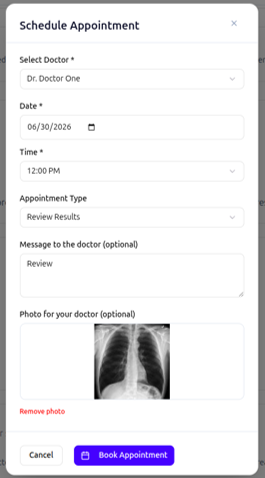
\includegraphics{assets/backend16.png}
	\caption{An image of the Schedule Appointment interaction from the system.}
	\label{fig:appointment_mgmt}
\end{figure}

\paragraph{Real-Time WebSocket}
Spring WebSocket with STOMP over SockJS provides live FL hospital status to the frontend. A scheduled poller runs every 10 seconds, fetches client status from the FL Server, syncs to PostgreSQL, and broadcasts to /topic/fl/clients. Hospital nodes that miss heartbeats are marked OFFLINE automatically.

\paragraph{Email Service}
Spring Mail with Gmail SMTP sends three types of emails:
\begin{itemize}
	\item Password Reset: link to \texttt{/reset-password?token=...}
	\item Admin Invite: link to \texttt{/set-password?token=...} for new doctor/admin accounts
	\item FL hospital onboarding: download link for the hospital Docker client package plus connection details.
\end{itemize}

\paragraph{Core API Modules}
The core modules exposed by the API and implemented in it a re listed in Table~\ref{tab:backend_modules}
\begin{table}[htbp]
	\centering
	\caption{Backend service modules and their responsibilities within the system.}
	\label{tab:backend_modules}
	\begin{tabular}{|p{4cm}|p{9cm}|}
		\hline
		\textbf{Module} & \textbf{Description} \\
		\hline
		
		Authentication &
		Handles the full authentication lifecycle including user registration, login, token issuance, refresh token management, and logout operations. \\
		\hline
		
		Image Upload &
		Generates and returns Cloudflare R2 presigned PUT URLs to enable secure direct client-side uploads of medical images. \\
		\hline
		
		Image Processing &
		Orchestrates the machine learning inference pipeline, triggers model execution, and stores as well as retrieves diagnostic results from the persistence layer. \\
		\hline
		
		Appointments &
		Manages the full appointment workflow, allowing patients to book appointments and doctors to approve, complete, or cancel scheduled sessions. \\
		\hline
		
		Admin User Management &
		Provides administrative capabilities for managing user accounts, including creation, modification, role assignment, and deactivation. \\
		\hline
		
		Federated Learning Hospitals &
		Handles hospital registration and management within the federated learning ecosystem, acting as a proxy interface to the federated learning server. \\
		\hline
		
		Federated Learning Webhooks &
		Processes callback events from the federated learning server after training rounds, updating system state and storing training metadata accordingly. \\
		\hline
		
	\end{tabular}
\end{table}

\subsection{ML Service - ModelBackend}
ModelBackend is a FastAPI microservice that hosts all AI capabilities. At startup it loads four ML components into memory and exposes a unified image-processing endpoint plus a RAG chatbot. It runs on port 8000 and is called by centralized Backend for image analysis and directly by the frontend for chatbot interactions.

\subsubsection{ML Models}
Different backbone models were used for the different tasks the proposed system performs. All the AI models and architectures used are listed in Table~\ref{tab:ml_components}.

\begin{table}[htbp]
	\centering
	\caption{Machine learning components and their corresponding frameworks and purposes within the proposed system.}
	\label{tab:ml_components}
	\begin{tabular}{|p{4cm}|p{5cm}|p{6cm}|}
		\hline
		\textbf{Component} & \textbf{Framework} & \textbf{Purpose} \\
		\hline
		
		Router Model &
		Keras (DenseNet121) &
		Classifies input images into X-ray, CT scan, or out-of-distribution categories using 224×224 image resolution as the first stage of the diagnostic pipeline. \\
		\hline
		
		Chest Classification &
		TensorFlow/Keras (DenseNet121) &
		Performs four-class chest X-ray diagnosis including COVID-19, Normal, Pneumonia, and Tuberculosis classification in a multi-label-ready setup. \\
		\hline
		
		Lung Segmentation &
		TensorFlow/Keras (U-Net) &
		Extracts lung regions from medical images prior to classification to enhance focus on relevant anatomical structures and improve diagnostic accuracy. \\
		\hline
		
		Lung Cancer Detection &
		YOLOv8 &
		Detects and localizes lung cancer regions in CT scans using bounding box predictions for object-level medical diagnosis. \\
		\hline
		
		RAG Stack &
		LangChain, Ollama, and FAISS &
		Implements a retrieval-augmented generation chatbot for medical question answering using vector-based document retrieval and local LLM inference. \\
		\hline
		
	\end{tabular}
\end{table}

FastAPI serves as the AI engine of XFed NeuroScan and relies on Spring Boot to integrate its models into the complete healthcare platform. While FastAPI is responsible for running AI models and generating predictions, Spring Boot manages the workflow and communicates with the AI service whenever analysis is requested.

Separating Spring Boot and FastAPI into two services improves scalability and maintainability, allowing the healthcare system and AI models to be developed, updated, and deployed independently without affecting each other.

\subsubsection{Image Processing Pipeline}
The image processing module is designed to automatically analyze uploaded medical images and route them to the appropriate AI model based on their content. This architecture allows the system to support multiple diagnostic pipelines while maintaining a single entry point for image analysis.

\paragraph{Unified Routing}
Every uploaded image first passes through the Router Model, which serves as the initial classification layer. The router determines whether the image is a chest X-ray, lung cancer image, or an unsupported image type. A confidence threshold of 0.5 is used to ensure reliable routing decisions. Images classified as other are immediately rejected to prevent invalid data from being processed by diagnostic models. Once classified, chest X-rays are forwarded to the DenseNet-based chest disease pipeline, while lung cancer images are sent to the YOLOv8 detection pipeline.

\paragraph{Chest Pipeline}
The chest disease analysis pipeline is optimized for detecting four classes: COVID-19, Pneumonia, Tuberculosis, and Normal. Before classification, several preprocessing steps are applied to improve image quality and model performance.

First, a U-Net lung segmentation model isolates the lung region from the surrounding anatomy, allowing the classifier to focus only on clinically relevant areas. Next, Contrast Limited Adaptive Histogram Equalization (CLAHE) enhances local contrast within the segmented lungs, making subtle abnormalities easier to detect. A Gaussian Blur (5×5) filter is then applied to reduce image noise while preserving important structures.

The processed image is normalized to the range [0,1], converted to RGB format, and resized to 224×224 pixels, which matches the input requirements of the DenseNet model. The DenseNet classifier then predicts one of the four disease categories and returns a confidence score indicating prediction certainty.

To improve explainability, the system generates a Grad-CAM heatmap from the final convolutional layers of the network. This heatmap highlights the image regions that most influenced the model’s decision, providing visual evidence to support the prediction. Both the original image and the generated heatmap are uploaded to Cloudflare R2 for storage and later retrieval by the frontend.

\paragraph{Lung Cancer Pipeline}
The lung cancer pipeline is based on YOLOv8, an object detection model capable of identifying suspicious cancerous regions within medical images. After the router classifies an image as a lung cancer case, it is forwarded directly to the YOLOv8 model for inference.

The model performs real-time detection using a confidence threshold of 0.3, identifying potential cancer regions and generating bounding boxes around detected abnormalities. For each detected region, the model provides confidence scores indicating the likelihood of cancer presence.

The detected regions are then visually annotated on the image by drawing bounding boxes and labels, creating an interpretable result that can be reviewed by medical professionals. The final annotated image is uploaded to Cloudflare R2 under the lung cancer results directory, allowing it to be displayed in the frontend and stored as part of the patient's analysis history.

This dual-pipeline architecture combines classification-based diagnosis for chest diseases with object-detection-based localization for lung cancer, enabling the platform to provide both diagnostic predictions and visual explanations while maintaining a unified processing workflow.

An overall visualization of the image processing pipeline is shown in Figure~\ref{fig:backend_overall}

\begin{figure}[htbp]
	\centering
	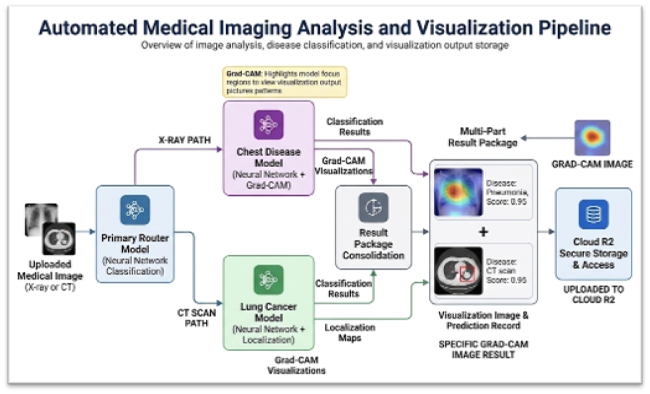
\includegraphics[width=0.95\linewidth]{assets/backend17.png}
	\caption{A simple visualization of the overall image processing pipeline from the backend's perspective.}
	\label{fig:backend_overall}
\end{figure}

\subsubsection{Grad-CAM Explainability and Localization}
For every chest X-ray prediction, the system generates a Grad-CAM (Gradient-weighted Class Activation Mapping) heatmap to provide interpretability for the AI decision. This mechanism highlights the regions of the image that most influenced the model’s prediction by tracing gradients flowing into the final convolutional layers of the DenseNet network.

The generated heatmap is visualized using a JET colormap and overlaid on the original X-ray image , allowing both the anatomical structure and the activated regions to remain clearly visible. This overlay helps radiologists and clinicians visually verify whether the model is focusing on medically relevant areas such as lung opacities, consolidations, or abnormal tissue patterns rather than irrelevant regions.

To support persistence and later retrieval, both the original Grad-CAM output and the processed overlay image are stored in Cloudflare R2 under the \texttt{heatmaps/} directory. These images are served to the frontend using secure presigned URLs, ensuring controlled and time-limited access to sensitive medical data.

\subsubsection{Localization Capability}Beyond explainability, Grad-CAM also provides a form of weak localization for disease regions within the chest X-ray. Although the DenseNet model is primarily designed for classification, Grad-CAM transforms it into a pseudo-localization system by identifying spatial regions that contribute most strongly to the predicted class.

This allows the system to:
\begin{itemize}
	\item Approximate the location of abnormal lung regions.
	\item Highlight areas associated with diseases.
	\item Provide spatial context without requiring a dedicated detection model   
\end{itemize}

In practice, this means the system not only predicts the presence of a disease but also indicates where in the lungs the abnormality is likely located. This improves clinical trust and makes the AI output more interpretable, bridging the gap between pure classification models and spatially aware diagnostic tools.

Overall, Grad-CAM serves as both an explainability mechanism and a lightweight localization method, enhancing transparency and clinical usability of the AI predictions.

\subsubsection{RAG Chatbot Module}
Retrieval-Augmented Generation (RAG) is an AI technique that enhances LLM responses by grounding them in a private document corpus rather than relying solely on the model's pre-trained knowledge. This is critical for domain-specific applications — such as medical systems,  where accuracy, traceability, and up-to-date information are essential.

\paragraph{Standard RAG Pipeline}
\begin{itemize}
	\item Ingest:  Load source documents (PDF, TXT, etc.)
	\item Chunk: Split long documents into overlapping smaller pieces.
	\item Embed: Convert each chunk to a dense numerical vector using a sentence embedding model.
	\item Store: Persist vectors in a FAISS vector database, organized by category.
	\item Retrieve: On a user query, embed the question and find the top-k most similar chunks.
	\item Generate: Pass the retrieved chunks and the question to the LLM to produce a grounded answer.
\end{itemize}

The classifier is the key differentiator of this RAG system. Rather than searching all documents indiscriminately, each query is first categorized, enabling targeted retrieval from the correct FAISS index.

\paragraph{Categories}
\begin{table}[htbp]
	\centering
	\caption{Categories of input handled by the RAG-based medical chatbot.}
	\label{tab:rag_input_categories}
	\begin{tabular}{|p{4cm}|p{9cm}|}
		\hline
		\textbf{Category} & \textbf{Typical Content} \\
		\hline
		
		Medical &
		Queries related to chest diseases and lung cancer, including symptoms, diagnosis, interpretation of medical findings, and general medical imaging questions. \\
		\hline
		
		General &
		Greetings, small talk, and off-topic or non-medical conversational queries that do not require clinical or diagnostic knowledge. \\
		\hline
		
	\end{tabular}
\end{table}

\paragraph{Model Architecture}
The classifier uses a lightweight 1D Convolutional Neural Network (CNN) designed for speed and bilingual text support, the full visualization of the architecture is shown in Figure~\ref{fig:rag_arch}.
\begin{enumerate}
	\item Input: Token IDs (max 50 tokens)
	\item Embedding Layer (vocab $\rightarrow$ 64 dims)
	\item Conv1d (64 $\rightarrow$ 128 channels) + ReLU + Dropout(0.3)
	\item Conv1d (128 $\rightarrow$ 128 channels) + ReLU
	\item AdaptiveMaxPool1d(1)
	\item Fully Connected: 128 $\rightarrow$ 64 $\rightarrow$ 3
	\item Output.
\end{enumerate}

\begin{figure}[htbp]
	\centering
	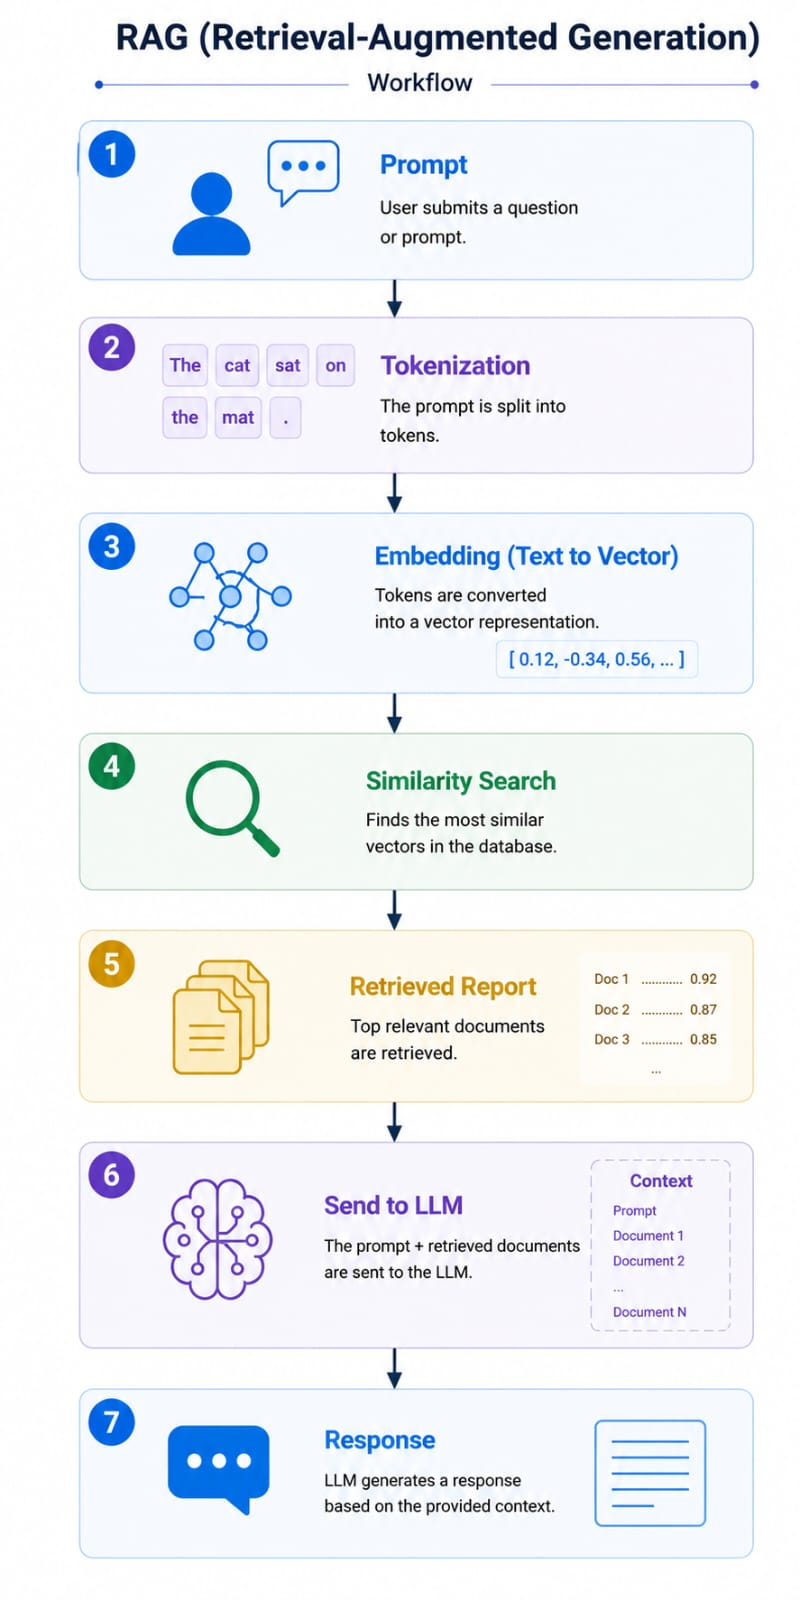
\includegraphics[height=0.90\textheight, keepaspectratio]{assets/backend18.jpeg}
	\caption{A simple visualization of the overall RAG architecture.}
	\label{fig:rag_arch}
\end{figure}

\paragraph{Bilingual Tokenizer}
\begin{itemize}
	\item Tokenizes Arabic , English, and numeric tokens
	\item Vocabulary built from training data (~300+ labeled question pairs)
	\item Fixed-length encoding: max 50 tokens, padded with <PAD>, unknown words as <UNK>
	\item Outputs: classifier.pth, tokenizer.json, config.json
\end{itemize}

\paragraph{Training Configuration}
The model was trained for 100 epochs using the Adam optimizer with a learning rate of 0.001 and a batch size of 16. The vocabulary size is 352 tokens, and each input token is mapped into a 64-dimensional embedding space. The hidden layer dimension is set to 128, Each input sequence is limited to a maximum length of 50 tokens to ensure consistent processing and performance.

\paragraph{LLM Configuration}
The configurations used for the RAG engine are shown in Table~\ref{tab:llm_parameters} for reproduce-ability purposes.
\begin{table}[htbp]
	\centering
	\caption{Configuration parameters of the RAG-based LLM engine.}
	\label{tab:llm_parameters}
	\begin{tabular}{|p{5cm}|p{8cm}|}
		\hline
		\textbf{Parameter} & \textbf{Standalone Value} \\
		\hline
		
		LLM Engine &
		Ollama \\
		\hline
		
		Model &
		qwen2.5:3b \\
		\hline
		
		Temperature &
		0.5 \\
		\hline
		
		Max Tokens &
		500 \\
		\hline
		
		Keep Alive &
		Infinite (-1) \\
		\hline
		
	\end{tabular}
\end{table}

\paragraph{Prompt Design}
The LLM is strictly instructed to answer only from the retrieved context. If the context does not contain the answer, the model is instructed to say "I don't know." Responses are capped at three sentences and must match the language of the question.

The text is split using a RecursiveCharacterTextSplitter with a chunk size of 1000 characters and an overlap of 150 characters between consecutive chunks. This ensures that the text is broken into manageable segments while preserving context between adjacent chunks for better retrieval accuracy.

RAG Independence from Image models  RAG does not receive chest X-ray predictions, GradCAM heatmaps, lung cancer results, or Spring Boot patient records. It is a standalone medical Q\&A chatbot co-located in every page  purely for deployment convenience.

Examples of using the RAG agent implemented in the system are shown in Figure~\ref{fig:rag_examples}

\begin{figure}[htbp]
	\centering
	
	% ---------------- Left Example ----------------
	\begin{subfigure}[t]{0.48\textwidth}
		\centering
		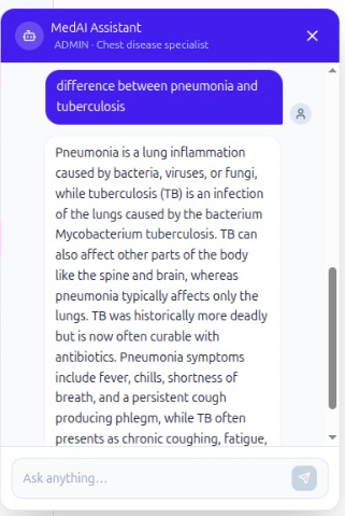
\includegraphics[width=\linewidth]{assets/backend19.png}
		\caption{Example of a medical query processed by the RAG agent, showing retrieval of relevant documents and generated response.}
		\label{fig:rag_example_1}
	\end{subfigure}
	\hfill
	% ---------------- Right Example ----------------
	\begin{subfigure}[t]{0.48\textwidth}
		\centering
		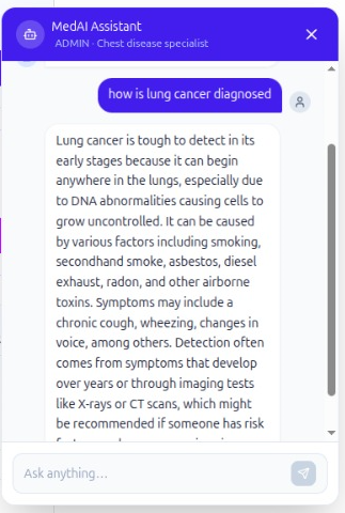
\includegraphics[width=\linewidth]{assets/backend20.png}
		\caption{Example of a general/off-topic query handled by the RAG agent with a conversational response without medical retrieval.}
		\label{fig:rag_example_2}
	\end{subfigure}
	
	\caption{Illustrative examples of the behavior of the retrieval-augmented generation (RAG) agent in different query scenarios. The system adapts its response strategy depending on whether the input is medical or general in nature.}
	\label{fig:rag_examples}
\end{figure}


\subsubsection{Performance Profile}
The performance profile of the proposed system is discussed in Table~\ref{tab:performance_overview}.
\begin{table}[htbp]
	\centering
	\caption{Computational performance and execution environment of the proposed system components.}
	\label{tab:performance_overview}
	\begin{tabular}{|p{5cm}|p{4cm}|p{5cm}|}
		\hline
		\textbf{Component} & \textbf{Approximate CPU Time} & \textbf{GPU} \\
		\hline
		
		Router &
		50--100 ms &
		Automatically enabled if CUDA is available \\
		\hline
		
		Chest Pipeline (Segmentation + Prediction + Grad-CAM) &
		1--5 s &
		CUDA auto-enabled \\
		\hline
		
		Lung Cancer YOLO Inference &
		1--5 s &
		CUDA auto-enabled \\
		\hline
		
		R2 Download / Upload &
		Network-dependent &
		N/A \\
		\hline
		
	\end{tabular}
\end{table}

Running the ModelBackend requires sufficient computational resources because it hosts multiple AI components simultaneously, including image classification models (DenseNet, YOLO, U-Net), the router model, and the RAG pipeline with embedding models and an LLM (Ollama). For stable performance, a GPU is strongly recommended for accelerating deep learning inference, especially for chest X-ray and lung cancer detection tasks.

In addition, the system requires adequate CPU resources to handle concurrent API requests, image preprocessing, and routing logic, while RAM (at least 4–6 GB minimum, higher recommended) is needed to keep multiple models, FAISS indexes, and embeddings loaded in memory without performance degradation. Overall, a balanced setup with a capable GPU, multi-core CPU, and sufficient RAM ensures smooth and responsive AI processing across all services in the ModelBackend

\subsection{Federated Learning Server}
The Federated-Learning-Server is responsible for enabling privacy-preserving collaborative training across multiple hospitals without requiring any centralization of medical data. It allows hospitals to jointly train a shared model while ensuring that raw patient images never leave their local environments, maintaining strict data privacy and compliance with healthcare constraints.

The system is built using a hybrid architecture that combines a FastAPI REST service and a Flower-based gRPC server within a single Python process. The FastAPI layer acts as the control interface for registration, monitoring, and coordination tasks, while the Flower server handles the actual federated learning workflow, including distributed training and weight aggregation.

Both components are synchronized through an in-memory SharedState singleton, which maintains the current training status, active clients, and round coordination signals. This design allows seamless communication between REST-based administrative actions and gRPC-based training execution, ensuring that federated learning rounds are executed in a coordinated and efficient manner across all participating hospitals.

\subsubsection{Design Principles}
The design principles of the federated learning server are listed in Table~\ref{tab:fl_principles}.
\begin{table}[htbp]
	\centering
	\caption{Core design principles and their implementation in the federated learning framework.}
	\label{tab:fl_principles}
	\begin{tabular}{|p{4cm}|p{9cm}|}
		\hline
		\textbf{Principle} & \textbf{Implementation} \\
		\hline
		
		Privacy first &
		Only model weight updates are transmitted between clients and the server; raw medical images never leave the hospital premises under any circumstance. \\
		\hline
		
		On-demand training &
		The Flower server remains idle until explicitly triggered by an administrator via the \texttt{POST /start-round} endpoint, ensuring that training rounds are fully controlled and non-automatic. \\
		\hline
		
		In-process coupling &
		FastAPI and Flower operate within a shared runtime environment using a \texttt{SharedState} singleton, eliminating the need for internal HTTP communication and reducing overhead. \\
		\hline
		
		Weight hot-reload &
		After each federated aggregation round, the updated global model weights are immediately pushed to the Model Backend, enabling real-time deployment of improved models. \\
		\hline
		
	\end{tabular}
\end{table}

The Federated-Learning-Server follows a dual-process architecture where two interconnected services run simultaneously within the same system. The main process runs a Uvicorn-based FastAPI server on port 8001, which acts as the REST bridge responsible for hospital registration, client management, monitoring, and handling webhooks from the main backend system. In parallel, a daemon process runs a Flower gRPC server on port 50051, which is responsible for coordinating the actual federated learning workflow, including distributed training and model weight aggregation across participating hospitals.

This separation allows the system to clearly divide responsibilities between control-plane operations (handled by FastAPI) and training-plane execution (handled by Flower). Both processes share a common in-memory SharedState, ensuring synchronization between REST actions and federated learning events while maintaining efficient and real-time coordination.

\subsubsection{Training Round Lifecycle}
A complete federated training round follows these steps:
\begin{itemize}
	\item Step 1: Admin selects online hospitals and initiates a round
	\item Step 2: Spring calls start-round with round id, min clients, deadline minutes
	\item Step 3: FastAPI sets SharedState \texttt{trigger\_event}, unblocking the Flower server thread
	\item Step 4: Hospital clients receive global weights via gRPC, train locally on their data
	\item Step 5: CustomFedAvg aggregates weight updates using the FedAvg algorithm
	\item Step 6: Aggregated weights saved and pushed to ModelBackend
	\item Step 7: Webhook notifies spring of round completion or failure
	\item Step 8: trigger event cleared; Flower waits for the next admin trigger
\end{itemize}

\begin{figure}[htbp]
\centering
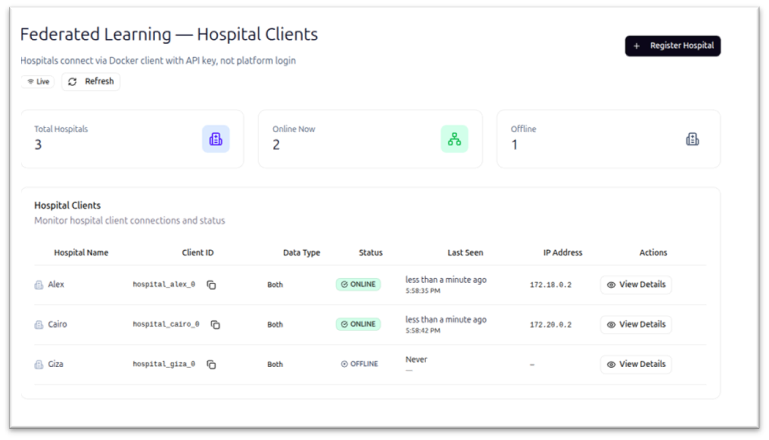
\includegraphics[width=0.95\linewidth]{assets/backend21.png}
\caption{The federated learning dashboard of the web application.}
\label{fig:fed_db}
\end{figure}

After a hospital is successfully registered in the federated learning system, Spring Boot finalizes the onboarding process by generating the necessary FL credentials and preparing a deployment package for that hospital. Once the registration is approved, the system automatically sends an email notification to the hospital using Gmail SMTP.

This email contains all essential onboarding information, including the hospital’s federated learning client ID, encrypted API key, and instructions for connecting to the Federated Learning Server. It also provides a Docker-based hospital client package, which is the only component the hospital needs to run locally.

From the hospital side, the setup process is intentionally simple. The hospital team only needs to:
\begin{enumerate}
	\item Put the data in the required folder
	\item Run the container provided in the package 
\end{enumerate}

Once the container is started, the hospital client automatically connects to the Federated Learning Server, begins sending heartbeat signals, and becomes eligible for participation in training rounds. After this step, no further manual integration is required, as all communication and training coordination are handled automatically by the system.

This design ensures a smooth onboarding process where hospitals do not need to manage complex machine learning setups, and can join the federated learning network by simply configuring and running a pre-built container

Once the container is running and sending heartbeat signals, the hospital is marked as ONLINE and becomes eligible to participate in federated training rounds.

\begin{figure}[htbp]
	\centering
	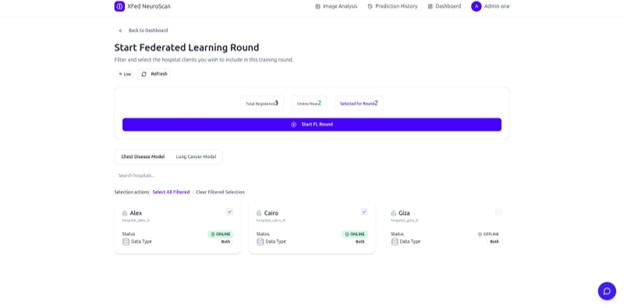
\includegraphics[width=0.95\linewidth]{assets/backend22.jpg}
	\caption{The federated learning management tab.}
	\label{fig:fed_mgmt}
\end{figure}

\subsubsection{Round Status States}
The full states and status code for the federated learning server are listed and explained in Table~\ref{tab:fl_status}
\begin{table}[htbp]
	\centering
	\caption{Federated learning server execution states and their meanings.}
	\label{tab:fl_status}
	\begin{tabular}{|p{3.5cm}|p{10cm}|}
		\hline
		\textbf{Status} & \textbf{Meaning} \\
		\hline
		
		IDLE &
		No federated learning round is currently running; the Flower server is blocked and waiting for an external trigger event. \\
		\hline
		
		STARTED &
		A training round has been triggered and participating hospital clients are actively performing local model training. \\
		\hline
		
		AGGREGATING &
		The server is performing FedAvg aggregation over received client updates to compute the new global model. \\
		\hline
		
		COMPLETED &
		The federated learning round has successfully finished, and the updated global model weights have been saved and pushed to the Model Backend for deployment. \\
		\hline
		
		FAILED &
		The federated learning round has failed due to issues such as timeouts, client-side errors, or model update push failures. \\
		\hline
		
	\end{tabular}
\end{table}

\subsubsection{Security}
The Federated Learning security model is designed to ensure strict isolation between hospitals, the platform backend, and the training infrastructure. A Platform API key is used exclusively by the centralized Backend to securely register new hospital clients, retrieve client lists, and initiate federated learning rounds, ensuring that only the trusted backend can control system-level operations.

Each hospital node is assigned a unique Client API key, which is used solely for heartbeat authentication to confirm that the hospital is online and eligible to participate in training. In addition, a Webhook secret is shared between the FL Server and centralized  Backend to verify and secure all outbound callbacks related to training round completion and status updates.

Hospitals communicate with the system only through outbound connections to port 8001 for REST heartbeats and port 50051 for gRPC-based training, eliminating the need for direct inbound access. Importantly, admin users never interact directly with the FL Server; instead, all operations are securely routed through centralized Backend using JWT authentication, maintaining a centralized and controlled security layer.

The various key types and their roles are shown and explained in great detail in Table~\ref{tab:fl_keys}.

\begin{table}[htbp]
	\centering
	\caption{Authentication key types and their roles within the federated learning system.}
	\label{tab:fl_keys}
	\begin{tabular}{|p{4cm}|p{4.5cm}|p{6cm}|}
		\hline
		\textbf{Key Type} & \textbf{Holder} & \textbf{Scope} \\
		\hline
		
		Platform API Key &
		Centralized Backend &
		Used by the backend system to register clients, initiate federated learning rounds, and retrieve the list of participating clients. \\
		\hline
		
		Client API Key &
		Each hospital node &
		Used exclusively for heartbeat authentication to verify active participation and connectivity of hospital clients. \\
		\hline
		
		Webhook Secret &
		Federated Learning Server and Centralized Backend &
		Used to authenticate outbound callback requests from the federated learning server after training rounds to ensure secure communication. \\
		\hline
		
	\end{tabular}
\end{table}

\subsection{End-to-End Data Flows}
\subsubsection{Medical Image Analysis Flow}
\begin{enumerate}
	\item The frontend user selects an image and requests a presigned URL from the Spring Backend.
	
	\item The frontend uploads the image directly to Cloudflare R2 using the provided presigned URL.
	
	\item After upload, the frontend calls the image processing service with the stored R2 key.
	
	\item The Spring Backend saves image metadata in PostgreSQL, generates a presigned URL, and forwards the request to the FastAPI service via Feign client communication.
	
	\item The FastAPI service downloads the image from R2, routes it using the trained routing model, and executes the appropriate specialist pipeline (either chest disease classification or lung cancer detection).
	
	\item The FastAPI service uploads the generated outputs (such as Grad-CAM heatmaps or annotated detection images) back to R2 and returns the prediction, confidence score, and storage key.
	
	\item The Spring Backend stores the final inference results in the database and generates presigned URLs for secure result visualization.
	
	\item The frontend displays the prediction results, confidence scores, and visual explanations such as Grad-CAM overlays or bounding box annotations to the user.
\end{enumerate}

\subsubsection{User Authentication Flow}
\begin{enumerate}
	\item The user logs in via the login page, where credentials are verified by Spring Security.
	
	\item If authentication succeeds, an access JWT is returned in the response body, and a refresh token is set as an HttpOnly cookie.
	
	\item The refresh token is also stored in Redis with a defined key and a 30-day expiration period.
	
	\item The frontend stores the access token in memory, while the authentication context initializes and loads the user role and profile information.
	
	\item When the access token expires, the frontend calls the refresh token endpoint, which issues a new access token and rotates the refresh cookie.
	
	\item During logout, the access token is blacklisted and the refresh token is removed from Redis, fully invalidating the user session.
\end{enumerate}

\subsubsection{Federated Learning Hospital Status Flow}
\begin{enumerate}
	\item The administrator registers a hospital through the frontend interface, and the Spring forwards the registration request to the Federated Learning (FL) Server.
	
	\item The FL Server generates a unique API key, which is encrypted and stored by the backend. Subsequently, an onboarding email containing the Docker-based client package is sent to the hospital.
	
	\item The hospital deploys the provided Docker client, which establishes a connection to the Flower server via gRPC for federated learning participation.
	
	\item The hospital client initiates a heartbeat process that continuously sends periodic signals to the FL Server every 30 seconds to indicate active status.
	
	\item The Spring Backend executes a polling mechanism every 10 seconds to retrieve the latest client status updates from the FL Server.
	
	\item The retrieved client statuses are synchronized with the PostgreSQL database and broadcast in real time using STOMP WebSocket communication.
	
	\item The frontend subscribes to the WebSocket channel and dynamically updates hospital ONLINE/OFFLINE indicators in real time based on received status updates.
\end{enumerate}


\section{Summary}

This chapter presented the proposed end-to-end model for automated detection of chest diseases and bone fractures from medical images. The overall solution architecture was introduced, highlighting the integration of a deep learning–based diagnostic pipeline with supporting backend processes to enable efficient and scalable medical image analysis.

The deep learning pipeline was described in detail, illustrating the sequential flow from image preprocessing and feature extraction to intelligent routing and task-specific inference. Transfer learning was adopted as a core strategy to leverage pre-trained deep neural networks, enabling effective feature representation and improved generalization in the presence of limited labeled medical data.

The chapter also introduced the medical image routing model, which enables dynamic task allocation by directing input images to specialized diagnostic models. This design enhances modularity and allows the system to support multiple medical imaging tasks within a unified framework.

Then, the architecture of the chest disease classification model was discussed in detail. The design was illustrated, and the use of ResNet50 as the main feature extractor was justified. The formulation of the problem and the motivation behind such a model were presented while detailed architectural aspects of the transfer-learning model were omitted to avoid redundancy.

Finally, the bone fracture detection model was presented as a task-specific component of the system, implemented using an unmodified YOLOv8 architecture. The formulation of the fracture detection problem and the motivation for adopting a one-stage object detection approach were discussed, while detailed architectural aspects were referenced to earlier sections to avoid redundancy.

Overall, this chapter established the structural and methodological foundation of the proposed system, providing a clear understanding of its components and design choices. The described models form the basis for the experimental evaluation and performance analysis presented in the subsequent chapter.
	
	%Chapter 4 Title page
	\vspace*{\fill} % Pushes content down from the top
	\thispagestyle{chapterpages}
	\begin{center} % Centers content horizontally
		\begin{minipage}{0.9\textwidth} % Creates a box for your text, adjust width as needed
			\centering % Centers text within the minipage
			{\color{RoyalBlue}\fontsize{30pt}{20pt}\bfseries\selectfont
				CHAPTER 4
				\\[0.2cm] RESULTS \& \\[0.2cm] EVALUATION
			}
		\end{minipage}
	\end{center}
	\vfill % Pushes content up from the bottom (equivalent to \vspace{\fill})
	\newpage
	
	% Chapter 4 content
	\chapter{Results and Evaluation}

This chapter presents the experimental results obtained from the implementation and evaluation of the proposed framework, \textit{X-Fed NeuroScan: Federated Learning with Explainable AI for Medical Image Classification}. The primary objective of this chapter is to assess the effectiveness of the developed models, validate the design decisions discussed in previous chapters, and demonstrate the capability of the proposed system to accurately analyze medical images within a hierarchical diagnostic pipeline.

The evaluation process was designed to investigate both the individual performance of each model and the overall effectiveness of the integrated framework. Since the proposed architecture consists of multiple interconnected components, a comprehensive assessment is necessary to ensure that each stage performs its intended function reliably. Particular emphasis is placed on the routing model, which serves as the first level of the classification pipeline and is responsible for identifying the modality of incoming medical images before directing them to the appropriate downstream diagnostic model. The performance of the disease classification and lung cancer detection models is subsequently analyzed to determine their ability to perform accurate medical image diagnosis within their respective domains.

To provide a rigorous and objective evaluation, multiple performance metrics are employed throughout this chapter. These metrics include accuracy, precision, recall, F1-score, loss values, confusion matrices, and training convergence behavior. In addition, comparative experiments are conducted to evaluate different model architectures and hyperparameter configurations, allowing the selection of the most suitable models for inclusion within the final framework. Training and validation curves are also examined to assess optimization stability, convergence characteristics, and generalization performance.

Beyond predictive performance, this chapter also evaluates the practical aspects of the proposed framework. The effectiveness of transfer learning, data augmentation, class balancing strategies, and other implementation choices is analyzed to determine their contribution to overall model performance. Furthermore, the results obtained from the explainability component are discussed to demonstrate how visual explanations can enhance model transparency and improve the interpretability of diagnostic decisions. The chapter also examines the federated learning implementation and its ability to support collaborative model training while preserving data privacy.

The results presented throughout this chapter provide quantitative and qualitative evidence regarding the feasibility of the proposed approach for medical image analysis. By systematically evaluating each component of the framework and comparing alternative design choices, this chapter establishes the effectiveness of the developed system and provides a foundation for the discussion, conclusions, and future research directions presented in the subsequent chapters.

\section[Routing Model Results]{Evaluation of the Medical Image Routing Model}

The medical image routing model represents the first level of the proposed hierarchical diagnostic framework and therefore plays a critical role in determining the overall effectiveness of the system. Since all incoming images must first pass through the routing stage before being analyzed by specialized diagnostic models, the reliability of this component directly impacts the performance of the entire framework. Consequently, a comprehensive evaluation was conducted to assess the ability of the routing model to accurately distinguish between chest X-ray images, chest CT scan images, and out-of-distribution images categorized as \emph{Other}.

The evaluation process was designed not only to measure the classification performance of the final selected model but also to compare multiple candidate architectures and investigate the effect of hyperparameter selection on model performance. In particular, several deep learning architectures were trained and evaluated under identical experimental conditions, including a custom convolutional neural network, ResNet50, DenseNet121, and EfficientNetB3. The objective was to identify the architecture that offered the best combination of classification accuracy, generalization capability, and computational efficiency for the image routing task.

\subsection{Implementation Environment and Development Tools}

The routing model was implemented using the Python programming language and developed within a Jupyter Notebook environment. The deep learning pipeline was built using TensorFlow version 2.20.0 and Keras version 3.12.0, which provided the necessary functionality for constructing, training, and evaluating convolutional neural networks. Data preprocessing, dataset partitioning, performance evaluation, and metric computation were performed using Scikit-learn version 1.8.0.

Model training and experimentation were conducted on a workstation equipped with an NVIDIA RTX 2060 graphics processing unit (GPU). The availability of GPU acceleration significantly reduced training times and enabled the efficient evaluation of multiple candidate architectures and hyperparameter configurations. Table~\ref{tab:routing_tools} summarizes the software and hardware environment used during the implementation and evaluation process.

\begin{table}[H]
	\centering
	\caption{Software and hardware environment used for implementing the routing model.}
	\label{tab:routing_tools}
	\begin{tabular}{|l|l|}
		\hline
		\textbf{Component} & \textbf{Specification} \\
		\hline
		Programming Language & Python 3.12 \\
		\hline
		Deep Learning Framework & TensorFlow 2.20.0 \\
		\hline
		Neural Network API & Keras 3.12.0 \\
		\hline
		Machine Learning Library & Scikit-learn 1.8.0 \\
		\hline
		Development Environment & Jupyter Notebook \\
		\hline
		GPU & NVIDIA RTX 2060 \\
		\hline
	\end{tabular}
\end{table}

\subsection{Dataset Preparation and Experimental Setup}

The aggregated routing dataset consisted of three image categories corresponding to the target classes of the routing problem. The first category contained chest X-ray images, the second category contained chest CT scan images, and the third category consisted of out-of-distribution images grouped under the \emph{Other} class. The final dataset contained a total of 19,615 images distributed across the three classes as shown in Table~\ref{tab:routing_dataset_distribution}.

\begin{figure}[H]
	\centering
	
	% ---------------- LEFT: TABLE ----------------
	\begin{minipage}[c]{0.46\textwidth}
		\centering
		
		\captionof{table}{Class distribution of the routing dataset.}
		\label{tab:routing_dataset_distribution}
		
		\vspace{0.3cm}
		
		\begin{tabular}{|l|c|}
			\hline
			\textbf{Class} & \textbf{Number of Images} \\
			\hline
			Chest X-Ray & 7,123 \\
			\hline
			Chest CT Scan & 2,534 \\
			\hline
			Other & 9,958 \\
			\hline
			Total & 19,615 \\
			\hline
		\end{tabular}
		
	\end{minipage}
	\hfill
	% ---------------- RIGHT: FIGURE ----------------
	\begin{minipage}[c]{0.46\textwidth}
		\centering
		
		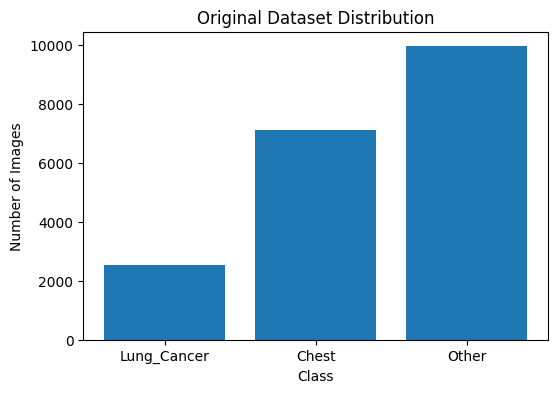
\includegraphics[
		width=\linewidth
		]{assets/dataset_dist_rm.png}
		
		\captionof{figure}{Distribution of the routing dataset classes.}
		\label{fig:routing_dataset_distribution}
		
	\end{minipage}
	
	\caption{Summary of the routing dataset distribution.}
	\label{fig:routing_dataset_summary}
\end{figure}

To ensure a fair evaluation procedure, the dataset was partitioned using a stratified sampling strategy. This approach preserved the original class distribution across all subsets and prevented sampling bias from influencing the evaluation results. The dataset was divided into training, validation, and testing subsets using a ratio of 70\%, 15\%, and 15\%, respectively.

A number of techniques were employed to mitigate the effects of class imbalance. First, class weights were incorporated during training to increase the contribution of minority classes to the optimization process. Second, stratified sampling was utilized to preserve representative class distributions across all dataset splits. Third, extensive data augmentation was applied to improve generalization and increase sample diversity. The augmentation pipeline included common image transformation techniques such as rotation, translation, zooming, flipping, brightness adjustment, and contrast variation. Geometric transformations that could significantly distort medical structures, such as excessive shearing, were intentionally avoided in order to preserve clinically relevant image features.

All models were trained using a batch size of 8 for a total of 10 epochs. The same training, validation, and testing partitions were used across all experiments to ensure consistency when comparing model performance.

\subsection{Learning Rate Optimization}

Since learning rate selection plays a crucial role in determining convergence behavior and final model performance, multiple learning rate values were investigated for each architecture. The evaluated learning rates included \(10^{-5}\), \(10^{-4}\), \(10^{-3}\), and \(10^{-2}\).

The experiments revealed that different architectures exhibited different optimization characteristics. DenseNet121 and ResNet50 achieved their highest performance when trained using a learning rate of \(10^{-2}\), whereas EfficientNetB3 performed best with a learning rate of \(10^{-4}\). Due to its relatively shallow architecture and limited feature extraction capacity, the custom convolutional neural network achieved its best results with a learning rate of \(10^{-5}\).

Table~\ref{tab:learning_rates} summarizes the optimal learning rate selected for each evaluated architecture.

\begin{table}[H]
	\centering
	\caption{Optimal learning rates identified during hyperparameter tuning.}
	\label{tab:learning_rates}
	\begin{tabular}{|l|c|}
		\hline
		\textbf{Model} & \textbf{Optimal Learning Rate} \\
		\hline
		Custom CNN & $10^{-5}$ \\
		\hline
		ResNet50 & $10^{-2}$ \\
		\hline
		DenseNet121 & $10^{-2}$ \\
		\hline
		EfficientNetB3 & $10^{-4}$ \\
		\hline
	\end{tabular}
\end{table}

These findings highlight the importance of architecture-specific hyperparameter tuning. Applying a common learning rate across all models would have resulted in suboptimal performance and potentially misleading comparisons between candidate architectures.

\subsection{Comparative Evaluation of Candidate Architectures}

To identify the most suitable backbone architecture for the routing model, four candidate architectures were trained and evaluated under identical conditions. The evaluated architectures included a custom CNN developed specifically for this task, ResNet50, DenseNet121, and EfficientNetB3.

The comparison focused on commonly used classification metrics, including accuracy, precision, recall, F1-score, and loss. Table~\ref{tab:routing_model_comparison} summarizes the performance of all evaluated architectures.

\begin{table}[H]
	\centering
	\caption{Performance comparison of candidate routing architectures.}
	\label{tab:routing_model_comparison}
	\begin{tabular}{|l|c|c|c|c|c|}
		\hline
		\textbf{Model} &
		\textbf{Accuracy} &
		\textbf{Precision} &
		\textbf{Recall} &
		\textbf{F1-Score} &
		\textbf{Loss} \\
		\hline
		Custom CNN & 1.0000 & 1.0000 & 1.0000 & 1.0000 & 0.0011 \\
		\hline
		ResNet50 & 1.0000 & 1.0000 & 1.0000 & 1.0000 & $1.782 \times 10^{-6}$ \\
		\hline
		EfficientNetB3 & 1.0000 & 1.0000 & 1.0000 & 1.0000 & $1.9816 \times 10^{-5}$ \\
		\hline
		DenseNet121 & 1.0000 & 1.0000 & 1.0000 & 1.0000 & $1.5126 \times 10^{-7}$ \\
		\hline
	\end{tabular}
\end{table}

The results demonstrate the superiority of DenseNet121 for the routing task. DenseNet121 achieved perfect classification performance on the test dataset, obtaining an accuracy, precision, recall, and F1-score of 100\%. Furthermore, the model achieved an extremely low loss value of \(1.5126 \times 10^{-7}\), indicating highly confident predictions and excellent convergence behavior.

The dense connectivity mechanism employed by DenseNet121 enables efficient feature reuse throughout the network and facilitates gradient propagation across deep layers. As a result, the model was able to learn highly discriminative representations that effectively separated the three image categories. Based on these findings, DenseNet121 was selected as the backbone architecture of the final routing model.

\begin{figure}[htbp]
	\centering
	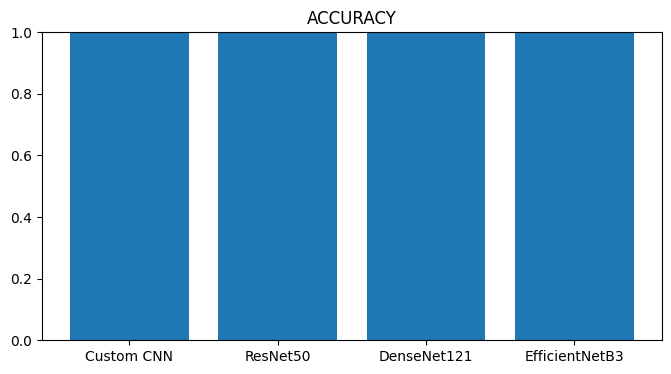
\includegraphics[width=\linewidth]{assets/models_acc_rm.png}
	\caption{Comparison of classification accuracy across all evaluated routing architectures.}
	\label{fig:routing_accuracy_comparison}
\end{figure}

\subsection{Training and Validation Behavior}

In addition to evaluating final classification performance, the training dynamics of each architecture were analyzed to assess convergence behavior and learning stability throughout the optimization process.

Figures~\ref{fig:routing_training_curves} illustrate the evolution of training accuracy, validation accuracy, training loss, and validation loss during the training process for all evaluated models.

\begin{figure}[htbp]
	\centering
	
	% -------------------------------------------------
	% Custom CNN
	% -------------------------------------------------
	\begin{subfigure}{0.95\textwidth}
		\centering
		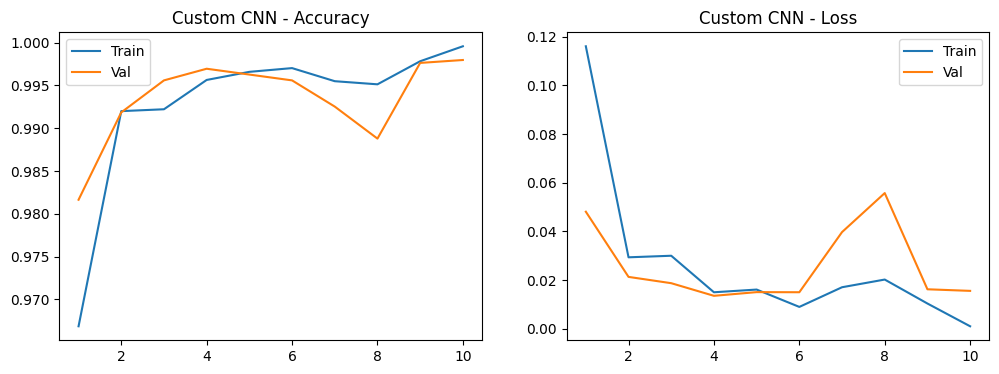
\includegraphics[
		width=\linewidth,
		height=0.18\textheight,
		keepaspectratio
		]{assets/curve_customcnn.png}
		\caption{Training and validation curves for the Custom CNN model.}
		\label{fig:customcnn_training_curves}
	\end{subfigure}
	
	\vspace{0.25cm}
	
	% -------------------------------------------------
	% ResNet50
	% -------------------------------------------------
	\begin{subfigure}{0.95\textwidth}
		\centering
		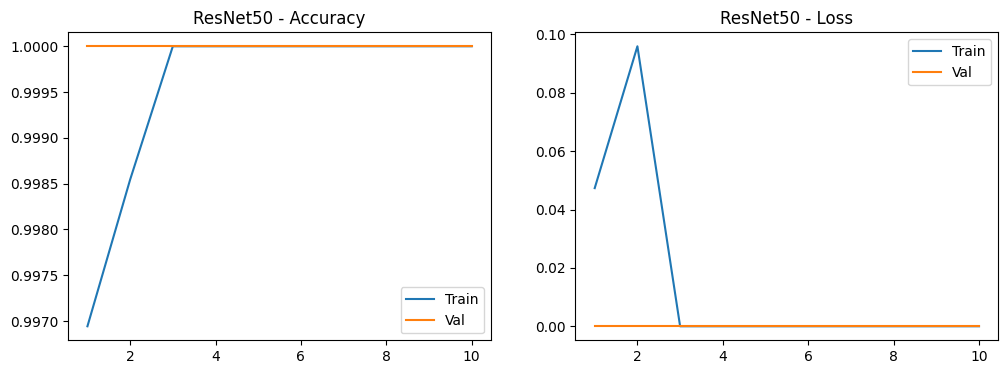
\includegraphics[
		width=\linewidth,
		height=0.18\textheight,
		keepaspectratio
		]{assets/curve_resnet.png}
		\caption{Training and validation curves for the ResNet50 model.}
		\label{fig:resnet50_training_curves}
	\end{subfigure}
	
	\vspace{0.25cm}
	
	% -------------------------------------------------
	% EfficientNetB3
	% -------------------------------------------------
	\begin{subfigure}{0.95\textwidth}
		\centering
		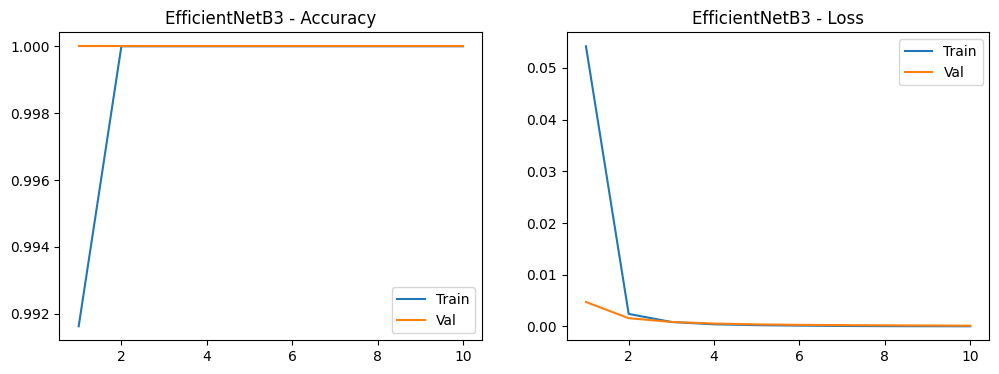
\includegraphics[
		width=\linewidth,
		height=0.18\textheight,
		keepaspectratio
		]{assets/curve_efficient.png}
		\caption{Training and validation curves for the EfficientNetB3 model.}
		\label{fig:efficientnet_training_curves}
	\end{subfigure}
	
	\vspace{0.25cm}
	
	% -------------------------------------------------
	% DenseNet121
	% -------------------------------------------------
	\begin{subfigure}{0.95\textwidth}
		\centering
		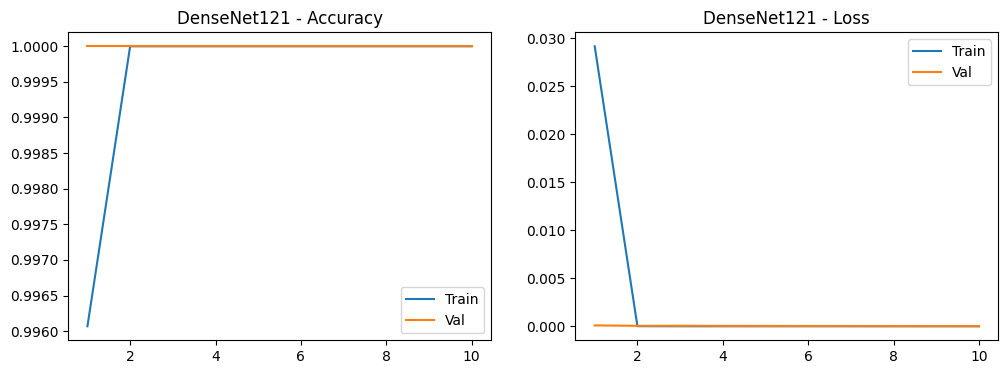
\includegraphics[
		width=\linewidth,
		height=0.18\textheight,
		keepaspectratio
		]{assets/curve_densenet.png}
		\caption{Training and validation curves for the DenseNet121 model.}
		\label{fig:densenet121_training_curves}
	\end{subfigure}
	
	\caption{Training and validation performance curves for all evaluated routing model architectures. Each figure illustrates the evolution of accuracy and loss throughout the training process and provides insight into model convergence, optimization stability, and generalization behavior.}
	\label{fig:routing_training_curves}
\end{figure}

Analysis of these curves provides valuable insight into convergence speed, optimization stability, and generalization behavior. The results indicate that DenseNet121 exhibited rapid convergence while maintaining stable validation performance throughout training, further supporting its selection as the final routing architecture.

\subsection{Confusion Matrix Analysis}

To further investigate classification performance, confusion matrices were generated for each evaluated architecture. Confusion matrices provide a detailed view of model predictions by illustrating the relationship between true class labels and predicted class labels.

The confusion matrix analysis is particularly important for the routing stage because misclassification at this level may cause images to be forwarded to an inappropriate downstream diagnostic model. Therefore, minimizing routing errors is essential for ensuring the reliability of the entire hierarchical framework.

Figure~\ref{fig:all_confusion_matrices} presents the confusion matrices obtained for all evaluated architectures.

\begin{figure}[htbp]
	\centering
	
	% ---------------- Row 1 ----------------
	\begin{subfigure}[t]{0.48\textwidth}
		\centering
		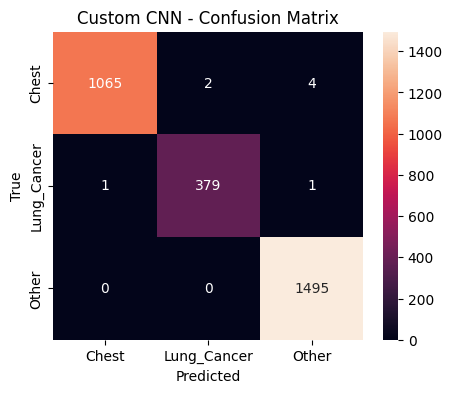
\includegraphics[
		width=\linewidth,
		height=0.28\textheight,
		keepaspectratio
		]{assets/customcnn_cm_rm.png}
		\caption{Custom CNN}
	\end{subfigure}
	\hfill
	\begin{subfigure}[t]{0.48\textwidth}
		\centering
		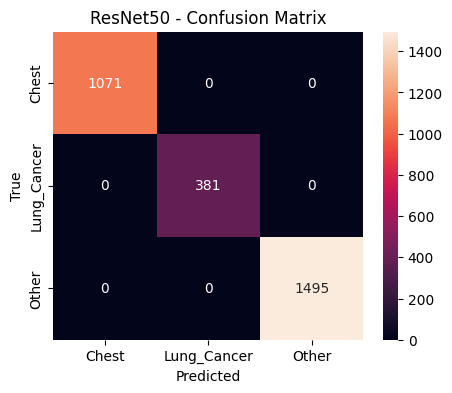
\includegraphics[
		width=\linewidth,
		height=0.28\textheight,
		keepaspectratio
		]{assets/resnet50_cm_rm.png}
		\caption{ResNet50}
	\end{subfigure}
	
	\vspace{0.3cm}
	
	% ---------------- Row 2 ----------------
	\begin{subfigure}[t]{0.48\textwidth}
		\centering
		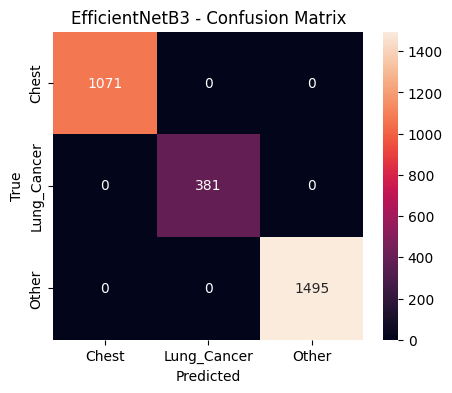
\includegraphics[
		width=\linewidth,
		height=0.28\textheight,
		keepaspectratio
		]{assets/efficient_cm_rm.png}
		\caption{EfficientNetB3}
	\end{subfigure}
	\hfill
	\begin{subfigure}[t]{0.48\textwidth}
		\centering
		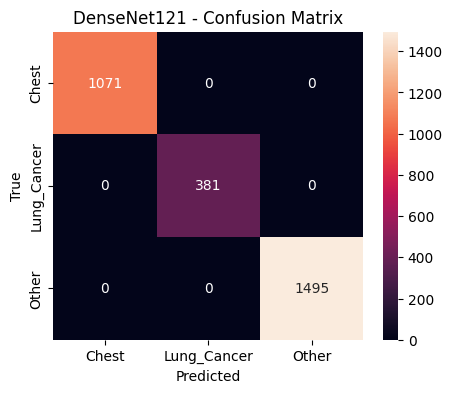
\includegraphics[
		width=\linewidth,
		height=0.28\textheight,
		keepaspectratio
		]{assets/densenet_cm_rm.png}
		\caption{DenseNet121}
	\end{subfigure}
	
	\caption{Confusion matrices for all evaluated routing models across the three classes.}
	\label{fig:all_confusion_matrices}
\end{figure}

The confusion matrix corresponding to DenseNet121 demonstrated perfect classification performance across all three classes, with no observed misclassifications in the test set. This result confirms the model's ability to accurately distinguish between chest X-ray images, chest CT scans, and out-of-distribution images, making it highly suitable for deployment as the first-level routing component within the proposed framework.

\subsection{Discussion}

The experimental results demonstrate that the proposed routing model successfully fulfills its intended objective of accurately identifying image modalities and directing images toward the appropriate diagnostic pathway. The combination of transfer learning, data augmentation, class weighting, and hyperparameter optimization enabled the evaluated architectures to achieve strong classification performance despite the inherent challenges associated with heterogeneous medical imaging data.

Among all tested architectures, DenseNet121 consistently produced the most favorable results and achieved perfect performance on the test dataset. The model's dense connectivity structure enabled efficient feature reuse and facilitated the extraction of highly discriminative modality-specific representations. Furthermore, the confusion matrix analysis confirmed the absence of routing errors, indicating that all images were successfully assigned to their correct categories.

These findings validate the effectiveness of the proposed first-level routing strategy and demonstrate that the routing component provides a reliable foundation for the subsequent disease classification and lung cancer detection stages of the overall framework.

% Relax float placement constraints for this section to improve page utilization
\renewcommand{\topfraction}{.85}
\renewcommand{\bottomfraction}{.7}
\renewcommand{\textfraction}{.15}
\renewcommand{\floatpagefraction}{.66}
\setcounter{topnumber}{9}
\setcounter{bottomnumber}{9}
\setcounter{totalnumber}{20}

\section{Chest Disease Classification Experiments}

This section documents the experimental results obtained from the evaluation of various deep learning architectures for chest disease classification. Both centralized and federated learning paradigms are explored to assess performance, generalization, and privacy-preserving capabilities.

\subsection{Implementation Environment and Development Tools}

This section documents the hardware infrastructure, software environment, and development frameworks employed throughout the experimental evaluation of the proposed chest disease classification system. Reproducibility of results depends critically on the precise specification of the computational environment, and accordingly all relevant configurations are reported below.

\subsubsection{Hardware Environment}

All centralized training experiments (preprocessing, U-Net segmentation, DenseNet121, ResNet50V2, EfficientNet, and VGG-19 classification models) were conducted on a cloud-based GPU accelerated computational environment. The hardware specifications and computed class weights are summarized in Table~\ref{tab:chest_hardware} and Table~\ref{tab:chest_computed_weights}, respectively.

{\renewcommand{\arraystretch}{1.2}
\begin{table}[htbp]
    \centering
    \begin{minipage}[c]{0.52\textwidth}
        \centering
        \caption{Hardware specifications.}
        \label{tab:chest_hardware}
        \small
        \begin{tabularx}{\textwidth}{|l|X|}
            \hline
            \textbf{Component} & \textbf{Specification} \\
            \hline
            Compute Platform & Colab Pro \\
            \hline
            GPU & NVIDIA T4 (15 GB) \\
            \hline
            CPU & Intel Xeon (2 vCPUs) \\
            \hline
            System RAM & 12--51 GB \\
            \hline
            Storage & Google Drive \\
            \hline
            OS & Ubuntu 20.04 LTS \\
            \hline
        \end{tabularx}
    \end{minipage}
    \hfill
    \begin{minipage}[c]{0.44\textwidth}
        \centering
        \caption{Computed class weights.}
        \label{tab:chest_computed_weights}
        \small
        \begin{tabularx}{\textwidth}{|l|c|X|}
            \hline
            \textbf{Class} & $N_k$ & \textbf{Weight $w_k$} \\
            \hline
            Normal & 4,870 & $\sim$0.78 \\
            \hline
            Pneu. & 4,221 & $\sim$0.90 \\
            \hline
            COVID & 3,192 & $\sim$1.19 \\
            \hline
            TB & 2,946 & $\sim$1.29 \\
            \hline
        \end{tabularx}
    \end{minipage}
\end{table}
}

The Federated Learning simulation experiments required more intensive multi-process resource management due to the Ray-based client parallelism used by the Flower framework. Resources were allocated per client using Ray's resource reservation mechanism, as detailed in Section~\ref{sec:federated_results}.

\subsubsection{Software Frameworks and Libraries}

The implementation stack is summarized in Table~\ref{tab:chest_software}. All dependencies were installed within the Colab environment, with version pinning applied where reproducibility was critical.

\begin{table}[htbp]
	\centering
	\caption{Software framework and library stack.}
	\label{tab:chest_software}
	\small
	\begin{tabularx}{\textwidth}{|l|l|X|}
		\hline
		\textbf{Library / Framework} & \textbf{Version / Source} & \textbf{Purpose} \\
		\hline
		Python & 3.10 & Primary programming language \\
		\hline
		TensorFlow / Keras & 2.15.1 & Centralized model training (U-Net, DenseNet, ResNet, EfficientNet, VGG) \\
		\hline
		PyTorch & 2.1.0 & Federated Learning model backbone (DenseNet121) \\
		\hline
		Torchvision & 0.16.1 & Pre-trained model weights, image transforms \\
		\hline
		Flower (flwr) & 1.4 (simulation) & Federated Learning framework (FedAvg strategy) \\
		\hline
		Ray & 2.1 & Distributed simulation backend for Flower \\
		\hline
		OpenCV (cv2) & 4.8.2 & Image preprocessing (CLAHE, Gaussian blur, normalization) \\
		\hline
		NumPy & 1.24.0 & Numerical computation \\
		\hline
		Scikit-learn & 1.3.0 & Classification reports, confusion matrices, AUC computation \\
		\hline
		Matplotlib & 3.7.1 & Training history plots, visualization \\
		\hline
		tqdm & 4.66.1 & Training progress bars \\
		\hline
		Pandas & 2.0.2 & Misclassification analysis and CSV export \\
		\hline
	\end{tabularx}
\end{table}

\subsubsection{Development Workflow}

All experiments were developed iteratively in Jupyter Notebooks within the Google Colab environment, with datasets mounted from Google Drive. The local preprocessing pipeline (CLAHE, Gaussian blur, normalization) was executed on a local machine equipped with an NVIDIA GPU, and the resulting processed dataset was uploaded to Google Drive for cloud-based training. Model checkpoints, final weights, and evaluation artefacts were saved both locally and to Drive for persistence across Colab session resets.

Mixed precision training (float16 for computations, float32 for master weights) was enabled throughout using TensorFlow's Automatic Mixed Precision (AMP) for TensorFlow experiments, providing approximately 2--3$\times$ speed improvement on Tensor Core-equipped NVIDIA GPUs with negligible accuracy impact.

\subsection{Dataset Preparation and Experimental Setup}

\subsubsection{Dataset Splits and Class Distribution}

The full composite dataset of 17,637 images was partitioned into training, validation, and test sets. The training set (15,229 images) was used exclusively for gradient-based parameter updates. The validation set was used for early stopping, learning rate scheduling, and model selection. The test set was kept strictly held out throughout all training and validation activities and was accessed only once for final performance evaluation.

{\renewcommand{\arraystretch}{1.2}
\begin{table}[htbp]
    \centering
    \begin{minipage}[c]{0.52\textwidth}
        \centering
        \caption{Complete dataset split.}
        \label{tab:chest_dataset_splits}
        \small
        \begin{tabularx}{\textwidth}{|l|c|c|c|c|}
            \hline
            \textbf{Class} & \textbf{Train} & \textbf{Val} & \textbf{Test} & \textbf{Total} \\
            \hline
            Normal & 4,870 & $\sim$610 & $\sim$610 & $\sim$6,090 \\
            \hline
            Pneu. & 4,221 & $\sim$528 & $\sim$528 & $\sim$5,277 \\
            \hline
            COVID & 3,192 & $\sim$400 & $\sim$400 & $\sim$3,992 \\
            \hline
            TB & 2,946 & $\sim$368 & $\sim$368 & $\sim$3,682 \\
            \hline
            \textbf{Total} & \textbf{15,229} & \textbf{1,906} & \textbf{1,906} & \textbf{19,041} \\
            \hline
        \end{tabularx}
    \end{minipage}
    \hfill
    \begin{minipage}[c]{0.44\textwidth}
        \centering
        \caption{Data augmentation parameters.}
        \label{tab:chest_augmentation}
        \small
        \begin{tabularx}{\textwidth}{|l|l|X|}
            \hline
            \textbf{Aug.} & \textbf{Param.} & \textbf{Just.} \\
            \hline
            Rotation & $\pm$15$^\circ$ & Position \\
            \hline
            W-Shift & $\pm$10\% & Lat. Trans. \\
            \hline
            H-Shift & $\pm$10\% & C-C Var. \\
            \hline
            Zoom & $\pm$10\% & SID Var. \\
            \hline
            H-Flip & $p=0.5$ & Symmetry \\
            \hline
            Fill & Zero & Textures \\
            \hline
        \end{tabularx}
    \end{minipage}
\end{table}
}

\textbf{Note on Class Imbalance:} The training set exhibits a moderate class imbalance, with Normal (32\%) substantially over-represented relative to Tuberculosis (19.3\%). Inverse-frequency class weights are applied during training for all models to counteract this imbalance and prevent the classifier from developing a bias toward more frequent classes.

\subsubsection{Data Augmentation Strategy}

Online data augmentation is applied exclusively to the training set using Keras's \texttt{ImageDataGenerator} API (for TensorFlow experiments) and \texttt{torchvision.transforms} (for Federated Learning experiments). The augmentation policy was carefully selected to apply only transformations that are plausible within the domain of chest radiography --- preserving diagnostic realism while increasing data diversity.

Notably, vertical flipping and brightness/contrast jitter are excluded to preserve diagnostic realism and avoid conflict with CLAHE preprocessing. Augmentations are applied only at training time; validation and test generators apply only the rescaling operation.

\subsubsection{Class Weighting}

To further address class imbalance beyond augmentation, inverse-frequency class weights are computed from the training set label distribution and passed to the model's \texttt{fit()} call. For each class $k$:
\begin{equation}
	w_k = \frac{N_{\text{total}}}{K \cdot N_k}
	\label{eq:chest_weights}
\end{equation}
where $K=4$, $N_{\text{total}}=15,229$, and $N_k$ is the number of training samples of class $k$. The computed weights for the training set are summarized in Table~\ref{tab:chest_computed_weights}.

\subsubsection{Evaluation Metrics}

Model performance is evaluated using a comprehensive set of metrics reflecting both overall and class-specific diagnostic performance:
\begin{itemize}
    \item \textbf{Accuracy:} $\frac{TP+TN}{TP+TN+FP+FN}$ --- overall proportion of correct predictions.
    \item \textbf{Precision (Positive Predictive Value):} $\frac{TP}{TP+FP}$ --- fraction of positive predictions that are correct.
    \item \textbf{Recall (Sensitivity):} $\frac{TP}{TP+FN}$ --- fraction of true positives correctly detected.
    \item \textbf{F1-Score:} $2 \cdot \frac{\text{Precision} \cdot \text{Recall}}{\text{Precision} + \text{Recall}}$ --- harmonic mean of precision and recall.
    \item \textbf{AUC-ROC:} Area under the Receiver Operating Characteristic curve (for OVR models, evaluated per class and macro-averaged).
    \item \textbf{Confusion Matrix:} A matrix showing the breakdown of correct and incorrect predictions across all class pairs.
\end{itemize}

\subsection{Segmentation Training Results}

The segmentation model was trained on a dataset of 6,106 annotated images, with an 85:15 split between training and validation sets. Early stopping was applied, terminating training at epoch 15 out of a maximum of 50 epochs. The model was optimized using the Adam optimizer with a learning rate of $10^{-4}$ and a combined Binary Cross-Entropy (BCE) and Dice loss function.

\begin{table}[h]
	\centering
	\caption{Segmentation Model Performance on the Validation Set}
	\label{tab:segmentation_results}
	\begin{tabular}{lc}
		\hline
		\textbf{Metric} & \textbf{Value} \\
		\hline
		Validation Accuracy & 95.86\% \\
		Training Accuracy & 98.14\% \\
		Validation Loss & 0.0904 \\
		Dice Coefficient & 0.9592 \\
		IoU Score & 0.9756 \\
		\hline
	\end{tabular}
\end{table}

The obtained results demonstrate excellent segmentation performance. The model achieved a validation accuracy of 95.86\% with a low validation loss of 0.0904, indicating good generalization capability. Furthermore, the Dice coefficient of 0.9592 and IoU score of 0.9756 confirm a high degree of overlap between the predicted masks and the ground-truth annotations, highlighting the effectiveness of the proposed segmentation approach.

\subsection{Single-Label Classification Results (SoftMax Approach)}

The SoftMax approach treats the four-class chest disease classification as a standard single-label multi-class problem: each image is assigned exactly one diagnostic class, and the output layer applies the SoftMax function to produce a valid probability distribution over the four classes:
\begin{equation}
	\hat{y}_k = \frac{e^{z_k}}{\sum_{j=1}^K e^{z_j}}, \quad \sum_{k=1}^K \hat{y}_k = 1
\end{equation}
The predicted class is $\hat{k} = \arg\max_k \hat{y}_k$, and the loss function is sparse categorical cross-entropy:
\begin{equation}
	\mathcal{L}_{\text{CE}} = -\log \hat{y}_{y_{\text{true}}}
\end{equation}

\subsubsection{DenseNet121 (SoftMax, Two-Phase Fine-Tuning)}

The first evaluated architecture is DenseNet121 with SoftMax output, trained using a two-phase fine-tuning strategy designed to maximize the transfer learning benefit while progressively adapting the network to the chest disease classification task. Key hyperparameters are detailed in Table~\ref{tab:densenet_softmax_params}. The learning curves, confusion matrix, and classification report for this model are shown in Figure~\ref{fig:densenet_softmax_curves}, Figure~\ref{fig:densenet_softmax_cm}, and Figure~\ref{fig:densenet_softmax_report}, respectively.

\textbf{Phase 1 --- Feature Extraction:} The DenseNet121 base is initialized with ImageNet weights. The last 100 layers are made trainable while all preceding layers are frozen. This selective unfreezing ensures that the early-stage feature extractors (which learn generic low-level features such as edges and textures --- applicable across domains) are preserved, while the deeper, task-specific layers are fine-tuned for chest pathology discrimination. The custom classification head (GAP $\to$ BN $\to$ Dense(512) $\to$ Dropout(0.4) $\to$ Dense(256) $\to$ Dropout(0.3) $\to$ Dense(4, SoftMax)) is trained end-to-end for a maximum of 40 epochs with the Adam optimizer at an initial learning rate of $10^{-4}$.

\textbf{Phase 2 --- Deep Fine-Tuning:} The best Phase 1 checkpoint is loaded, and the trainable scope is extended to the last 200 layers of the DenseNet121 base. The learning rate is significantly reduced to $10^{-6}$ (100$\times$ smaller) to ensure that the pre-trained weights are refined gently rather than disrupted. A maximum of 10 additional epochs are run. This two-phase strategy prevents the "catastrophic forgetting" of ImageNet representations that can occur when fine-tuning with an aggressive learning rate.

{\renewcommand{\arraystretch}{1.2}
\begin{table}[htbp]
	\centering
	\caption{DenseNet121 SoftMax --- Key Hyperparameters.}
	\label{tab:densenet_softmax_params}
	\small
	\begin{tabularx}{0.9\textwidth}{|X|l|l|}
		\hline
		\textbf{Parameter} & \textbf{Phase 1} & \textbf{Phase 2} \\
		\hline
		Trainable layers & Last 100 & Last 200 \\
		\hline
		Optimizer & Adam & Adam \\
		\hline
		Learning rate & $10^{-4}$ & $10^{-6}$ \\
		\hline
		Max epochs & 40 & 10 \\
		\hline
		Loss & \multicolumn{2}{l|}{Sparse Categorical Cross-Entropy} \\
		\hline
		Batch size & 32 & 32 \\
		\hline
		Early stopping & \multicolumn{2}{l|}{patience=8, monitor=val\_accuracy} \\
		\hline
		LR reduction & \multicolumn{2}{l|}{ReduceLROnPlateau (factor=0.2, patience=3)} \\
		\hline
	\end{tabularx}
\end{table}
}

\begin{figure}[htbp]
	\centering
	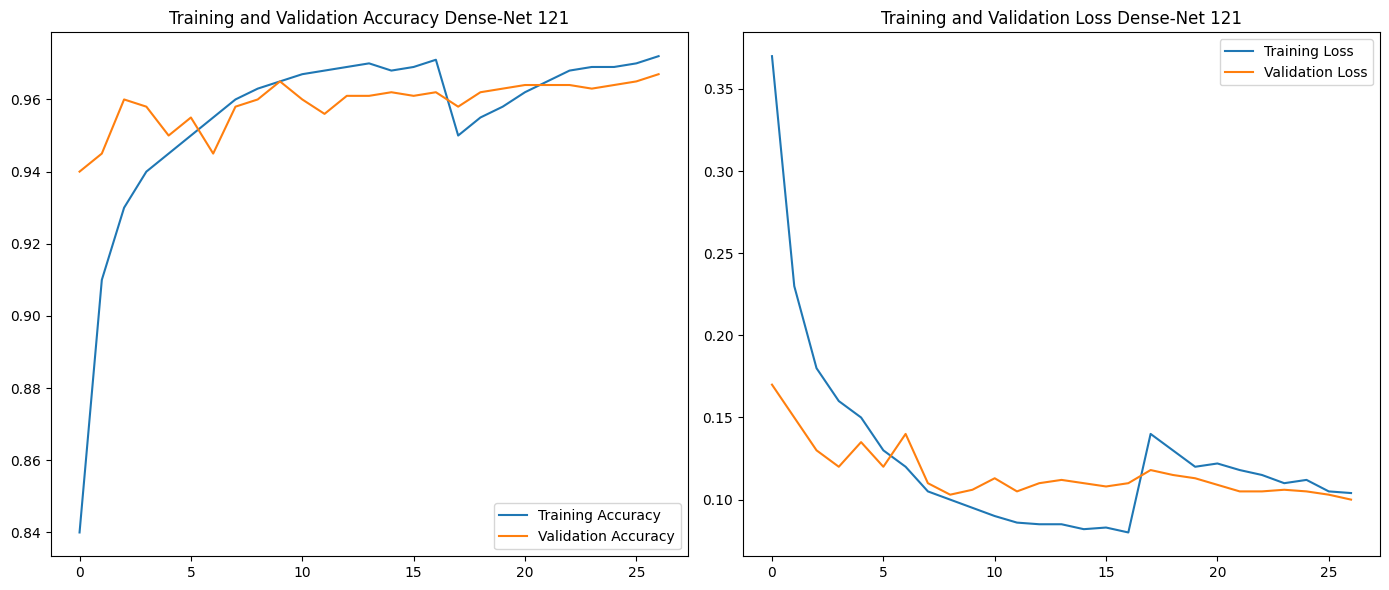
\includegraphics[width=0.85\textwidth, height=7cm, keepaspectratio]{assets/chest_model/image1.png}
	\caption{Learning curves for DenseNet121 SoftMax.}
	\label{fig:densenet_softmax_curves}
\end{figure}

\begin{figure}[htbp]
	\centering
	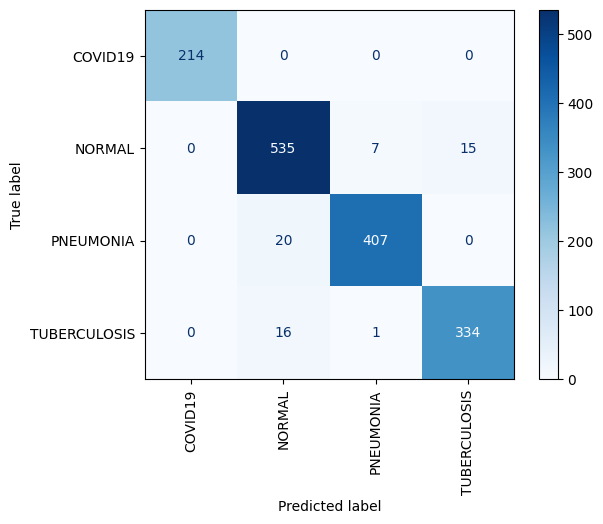
\includegraphics[width=0.7\textwidth, height=8cm, keepaspectratio]{assets/chest_model/image2.png}
	\caption{Confusion matrix for DenseNet121 SoftMax.}
	\label{fig:densenet_softmax_cm}
\end{figure}

\begin{figure}[htbp]
	\centering
	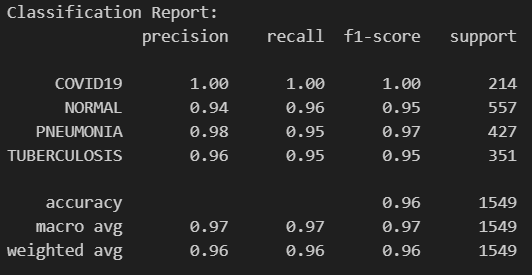
\includegraphics[width=0.85\textwidth, height=9cm, keepaspectratio]{assets/chest_model/image3.png}
	\caption{Classification report for DenseNet121 SoftMax.}
	\label{fig:densenet_softmax_report}
\end{figure}

\subsubsection{ResNet50V2 (Softmax, Partial Fine-Tuning)}

The second SoftMax baseline employs ResNet50V2 (He et al., 2016, V2 with pre-activation residual blocks), a 50-layer residual network pre-trained on ImageNet. ResNet50V2 introduces significant architectural improvements over the original ResNet50, including full pre-activation order (BN $\to$ ReLU $\to$ Conv rather than Conv $\to$ BN $\to$ ReLU), which leads to improved gradient flow and training stability. The model follows a partial fine-tuning strategy in which the last 40 layers are unfrozen for task-specific adaptation while the earlier layers retain their ImageNet representations.

The classification head follows the same structural template as DenseNet121: GAP $\to$ Dense(512, ReLU) $\to$ Dropout(0.4) $\to$ Dense(256, ReLU) $\to$ Dense(4, SoftMax). A notably lower learning rate of $10^{-4}$ is used from the outset, reflecting the more conservative fine-tuning approach appropriate for ResNet50V2's architecture. Key hyperparameters are listed in Table~\ref{tab:resnet_softmax_params}, with experimental results shown in Figure~\ref{fig:resnet_softmax_curves}, Figure~\ref{fig:resnet_softmax_cm}, and Figure~\ref{fig:resnet_softmax_report}. Training runs for a maximum of 30 epochs with early stopping (patience=7).

{\renewcommand{\arraystretch}{1.2}
\begin{table}[htbp]
	\centering
	\caption{ResNet50V2 SoftMax --- Key Hyperparameters.}
	\label{tab:resnet_softmax_params}
	\small
	\begin{tabularx}{0.85\textwidth}{|X|l|}
		\hline
		\textbf{Parameter} & \textbf{Value} \\
		\hline
		Base architecture & ResNet50V2 (ImageNet pre-trained) \\
		\hline
		Trainable layers & Last 40 layers + head \\
		\hline
		Frozen layers & First $\sim$145 layers \\
		\hline
		Optimizer & Adam ($10^{-4}$) \\
		\hline
		Max epochs & 30 \\
		\hline
		Loss & Sparse Categorical Cross-Entropy \\
		\hline
		Batch size & 32 \\
		\hline
		Early stopping & patience=7, monitor=val\_accuracy \\
		\hline
		LR reduction & ReduceLROnPlateau (factor=0.2, patience=3) \\
		\hline
	\end{tabularx}
\end{table}
}

\begin{figure}[htbp]
	\centering
	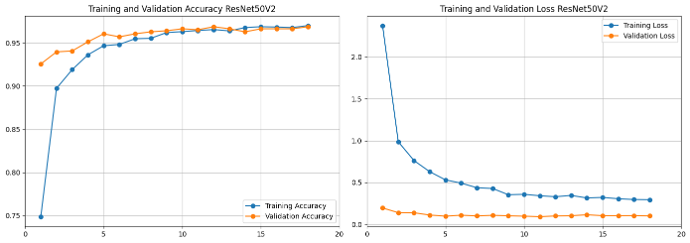
\includegraphics[width=\textwidth]{assets/chest_model/resnet-graphs.png}
	\caption{Learning curves for ResNet50V2 SoftMax.}
	\label{fig:resnet_softmax_curves}
\end{figure}

\begin{figure}[htbp]
	\centering
	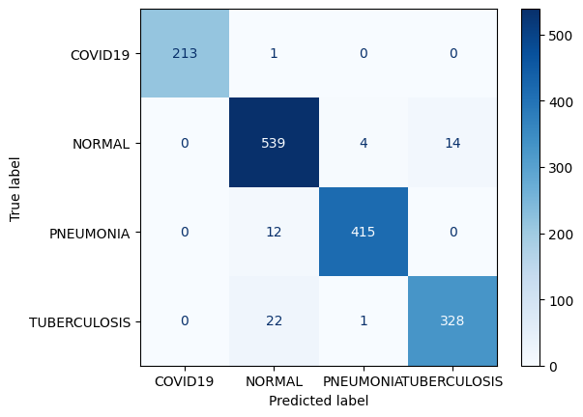
\includegraphics[width=\textwidth]{assets/chest_model/resnet-cm.png}
	\caption{Confusion matrix for ResNet50V2 SoftMax.}
	\label{fig:resnet_softmax_cm}
\end{figure}

\begin{figure}[htbp]
	\centering
	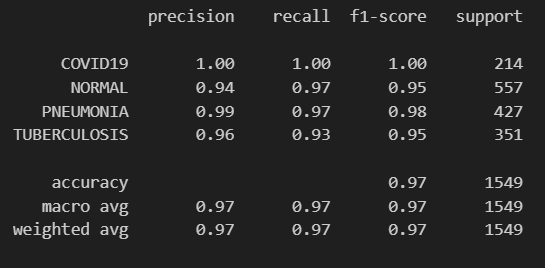
\includegraphics[width=0.85\textwidth, height=9cm, keepaspectratio]{assets/chest_model/image6.png}
	\caption{Classification report for ResNet50V2 SoftMax.}
	\label{fig:resnet_softmax_report}
\end{figure}

\FloatBarrier

\subsubsection{EfficientNet (SoftMax)}

EfficientNet scales network depth, width, and resolution jointly using a compound scaling coefficient, achieving state-of-the-art accuracy with fewer parameters than comparable architectures. The same classification head structure and training strategy are applied. Hyperparameters and results for EfficientNet are provided in Table~\ref{tab:efficientnet_softmax_params}, Figure~\ref{fig:efficientnet_softmax_curves}, Figure~\ref{fig:efficientnet_softmax_cm}, and Figure~\ref{fig:efficientnet_softmax_report}.

{\renewcommand{\arraystretch}{1.2}
\begin{table}[htbp]
	\centering
	\caption{EfficientNet SoftMax --- Key Hyperparameters.}
	\label{tab:efficientnet_softmax_params}
	\small
	\begin{tabularx}{0.85\textwidth}{|X|l|}
		\hline
		\textbf{Parameter} & \textbf{Value} \\
		\hline
		Base architecture & EfficientNetB0 (ImageNet pre-trained) \\
		\hline
		Trainable layers & Last 200 layers \\
		\hline
		Optimizer & Adam ($10^{-4}$) \\
		\hline
		Max epochs & 30 \\
		\hline
		Loss & Sparse Categorical Cross-Entropy \\
		\hline
		Batch size & 32 \\
		\hline
		Early stopping & patience=7, monitor=val\_accuracy \\
		\hline
		LR reduction & ReduceLROnPlateau (factor=0.2, patience=3) \\
		\hline
	\end{tabularx}
\end{table}
}

\begin{figure}[htbp]
	\centering
	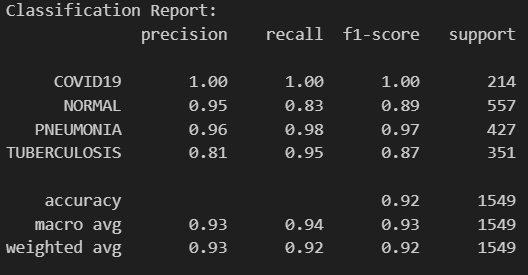
\includegraphics[width=0.85\textwidth, height=7cm, keepaspectratio]{assets/chest_model/image9.png}
	\caption{Classification report for EfficientNet SoftMax.}
	\label{fig:efficientnet_softmax_report}
\end{figure}

\begin{figure}[htbp]
	\centering
	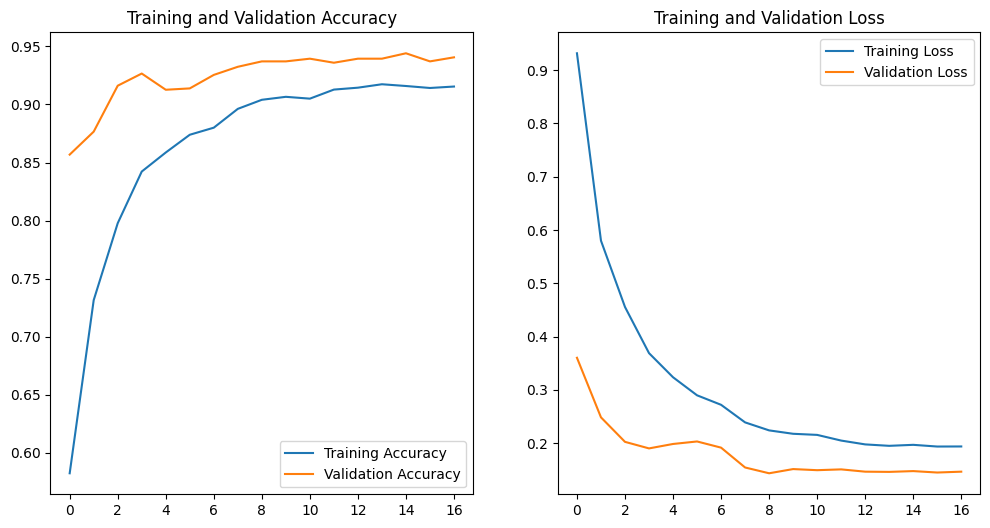
\includegraphics[width=\textwidth]{assets/chest_model/image7.png}
	\caption{Learning Curves for EfficientNet SoftMax.}
	\label{fig:efficientnet_softmax_curves}
\end{figure}

\begin{figure}[htbp]
	\centering
	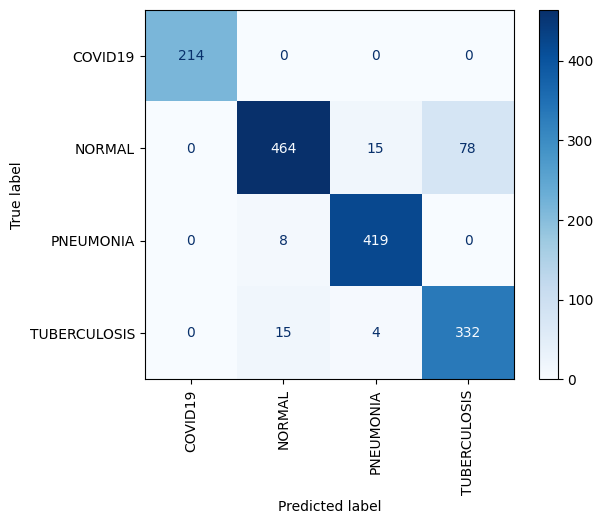
\includegraphics[width=\textwidth]{assets/chest_model/image8.png}
	\caption{Confusion matrix for EfficientNet SoftMax.}
	\label{fig:efficientnet_softmax_cm}
\end{figure}

\FloatBarrier

\subsubsection{VGG-19 (SoftMax)}

VGG-19 is a deep convolutional network with 19 weight layers characterized by a uniform architecture of convolutions and max-pooling operations. Despite its comparatively large parameter count, it remains a strong baseline for medical image classification due to its simple and well-understood feature hierarchy. Hyperparameters for VGG-19 are summarized in Table~\ref{tab:vgg_softmax_params}.

{\renewcommand{\arraystretch}{1.2}
\begin{table}[htbp]
	\centering
	\caption{VGG-19 SoftMax --- Key Hyperparameters.}
	\label{tab:vgg_softmax_params}
	\small
	\begin{tabularx}{0.85\textwidth}{|X|l|}
		\hline
		\textbf{Parameter} & \textbf{Value} \\
		\hline
		Base architecture & VGG-19 (ImageNet pre-trained) \\
		\hline
		Trainable layers & Last 5 conv layers + head \\
		\hline
		Optimizer & Adam ($10^{-5}$) \\
		\hline
		Max epochs & 30 \\
		\hline
		Loss & Sparse Categorical Cross-Entropy \\
		\hline
		Batch size & 32 \\
		\hline
		Early stopping & patience=7, monitor=val\_accuracy \\
		\hline
		LR reduction & ReduceLROnPlateau (factor=0.2, patience=3) \\
		\hline
	\end{tabularx}
\end{table}
}

Table~\ref{tab:vgg_res} presents the results achieved by the VGG-19 model configured with a Softmax activation function for multi-class chest disease classification. Overall, the model demonstrates strong discriminative capability across the four target classes (COVID-19, Normal, Pneumonia, and Tuberculosis), benefiting from the deep hierarchical feature extraction of the VGG-19 architecture. However, compared to more recent architectures, a slight reduction in generalization performance can be observed, particularly in visually similar classes such as Pneumonia and Tuberculosis, which often share overlapping radiographic patterns and therefore present a more challenging classification boundary.

The training dynamics of the model were recorded during training and are illustrated in Figure~\ref{fig:vgg_curves}, showing a generally stable convergence with steadily improving training and validation accuracy across epochs. A small generalization gap emerges in later epochs, indicating mild overfitting typical of high-capacity CNNs trained on limited medical datasets. The confusion matrix in Figure~\ref{fig:vgg-cm} further details class-wise prediction behavior, highlighting that most misclassifications occur between Pneumonia and Tuberculosis due to their radiographic similarity, while COVID-19 samples are classified more consistently due to more distinctive visual patterns. In addition, the final classification report shown in Figure~\ref{fig:vgg-report} confirms strong precision, recall, and F1-scores across most classes, providing a comprehensive evaluation of the model’s diagnostic performance.

\begin{table}[H]
	\centering
	\caption{Training Configuration and Performance Summary}
	\label{tab:vgg_res}
	\renewcommand{\arraystretch}{1.2}
	\begin{tabular}{|l|l|}
		\hline
		\textbf{Parameter} & \textbf{Value} \\
		\hline
		Loss & Sparse Categorical Cross-Entropy \\
		\hline
		Early stopping & patience = 5, monitor = val\_acc \\
		\hline
		LR reduction & factor = 0.1, patience = 4, min\_lr = $1 \times 10^{-7}$ \\
		\hline
		Accuracy & \textbf{94.77\%} \\
		\hline
	\end{tabular}
\end{table}

\begin{figure}[H]
	\centering
	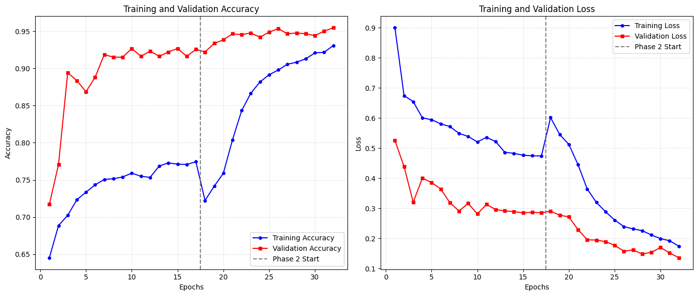
\includegraphics[width=\linewidth]{assets/chest_model/vgg-curves.png}
	\label{fig:vgg_curves}
	\caption{Learning curves for VGG-19 SoftMax.}
\end{figure}

\begin{figure}[H]
	\centering
	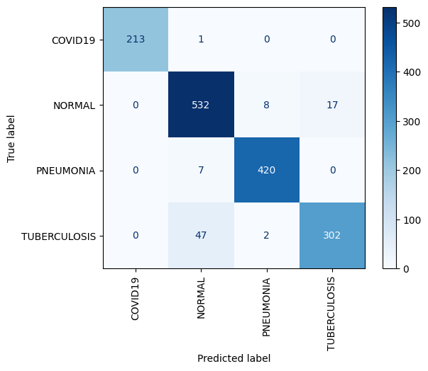
\includegraphics{assets/chest_model/vgg-cm.png}
	\label{fig:vgg-cm}
	\caption{Confusion matrix for VGG-19 SoftMax.}
\end{figure}

\begin{figure}[H]
	\centering
	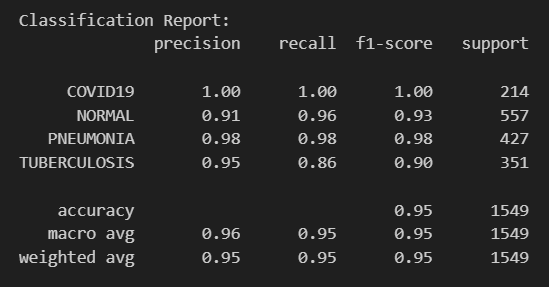
\includegraphics{assets/chest_model/vgg-report.png}
	\label{fig:vgg-report}
	\caption{Classification report for VGG-19 SoftMax.}
\end{figure}

\subsection{One-vs-Rest Classification Results (OVR / Sigmoid Approach)}

In the One-vs-Rest (OVR) paradigm, the four-class classification problem is decomposed into four independent binary classification sub-problems. Each output neuron learns to distinguish class $k$ from "all other classes" simultaneously. The output layer applies the sigmoid activation function independently to each logit, producing uncoupled probability scores:
\begin{equation}
	\hat{y}_k = \sigma(z_k) = \frac{1}{1 + e^{-z_k}}, \quad k \in \{1,2,3,4\}
\end{equation}
A threshold of 0.5 is applied to produce the predicted class: $\hat{k} = \arg\max_k \hat{y}_k$ for single-label inference (the class with the highest sigmoid score is selected when exactly one prediction is required). The training loss is Binary Cross-Entropy computed independently per class and per sample:
\begin{equation}
	\mathcal{L}_{\text{OVR}} = -\frac{1}{NK} \sum_{n=1}^N \sum_{k=1}^K \left[ y_{nk} \log \hat{y}_{nk} + (1 - y_{nk}) \log (1 - \hat{y}_{nk}) \right]
\end{equation}
Model selection is performed by monitoring the multi-label AUC-ROC metric on the validation set, rather than accuracy, because AUC is more informative for imbalanced multi-label settings.

\subsubsection{ResNet50 OVR (Sigmoid)}

The ResNet50 OVR model uses ResNet50 (original V1 architecture) as the backbone, with the last 40 layers unfrozen for fine-tuning. This is a more targeted fine-tuning scope than the SoftMax ResNet50V2 variant, focusing on the highest-level residual blocks that encode the most abstract and class-discriminative representations. The classification head follows the OVR template: GAP $\to$ BN $\to$ Dense(512, ReLU) $\to$ Dropout(0.4) $\to$ Dense(256, ReLU) $\to$ Dropout(0.3) $\to$ Dense(4, Sigmoid). Implementation details and results are given in Table~\ref{tab:resnet_ovr_params}, Figure~\ref{fig:resnet_ovr_curves}, Figure~\ref{fig:resnet_ovr_cm}, and Table~\ref{tab:resnet_ovr_report}.

{\renewcommand{\arraystretch}{1.2}
\begin{table}[htbp]
	\centering
	\caption{ResNet50 OVR --- Key Hyperparameters.}
	\label{tab:resnet_ovr_params}
	\small
	\begin{tabularx}{0.85\textwidth}{|X|l|}
		\hline
		\textbf{Parameter} & \textbf{Value} \\
		\hline
		Base architecture & ResNet50 (ImageNet pre-trained) \\
		\hline
		Trainable layers & Last 40 layers \\
		\hline
		Optimizer & Adam ($10^{-4}$) \\
		\hline
		Max epochs & 40 \\
		\hline
		Loss & Binary Cross-Entropy \\
		\hline
		Output activation & Sigmoid (independent) \\
		\hline
		Primary metric & AUC (multi-label) \\
		\hline
		Batch size & 32 \\
		\hline
	\end{tabularx}
\end{table}
}

\renewcommand{\arraystretch}{1.2}

\begin{table}[htbp]
	\centering
	\caption{ResNet50 OVR Report.}
	\label{tab:resnet_ovr_report}
	\small
	\begin{tabularx}{0.6\textwidth}{|X|c|c|c|}
		\hline
		\textbf{Class} & \textbf{Prec.} & \textbf{Rec.} & \textbf{F1} \\
		\hline
		COVID & 1.00 & 1.00 & 1.00 \\
		\hline
		Normal & 0.93 & 0.97 & 0.95 \\
		\hline
		Pneu. & 0.99 & 0.98 & 0.98 \\
		\hline
		TB & 0.97 & 0.91 & 0.94 \\
		\hline
		\textbf{Acc.} & \multicolumn{3}{c|}{\textbf{0.96}} \\
		\hline
	\end{tabularx}
\end{table}

\begin{figure}[htbp]
	\centering
	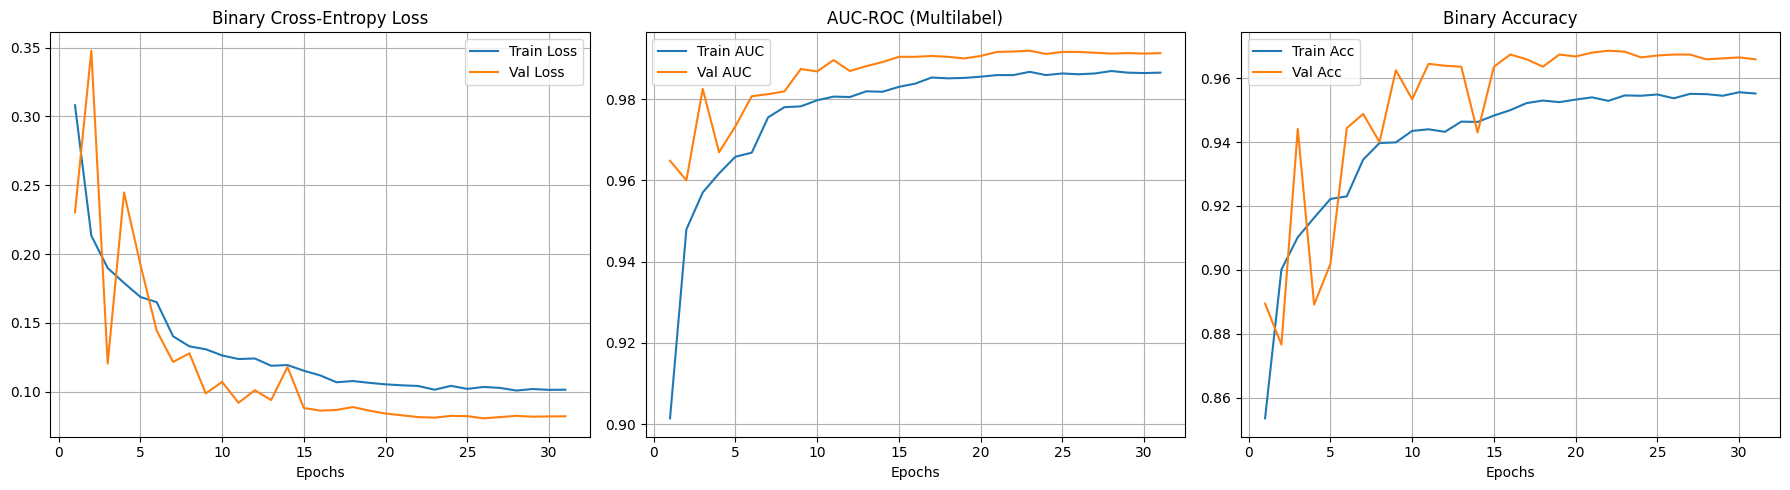
\includegraphics[width=\textwidth]{assets/chest_model/image10.png}
	\caption{Learning curves for ResNet50 OVR.}
	\label{fig:resnet_ovr_curves}
\end{figure}

\begin{figure}[htbp]
	\centering
	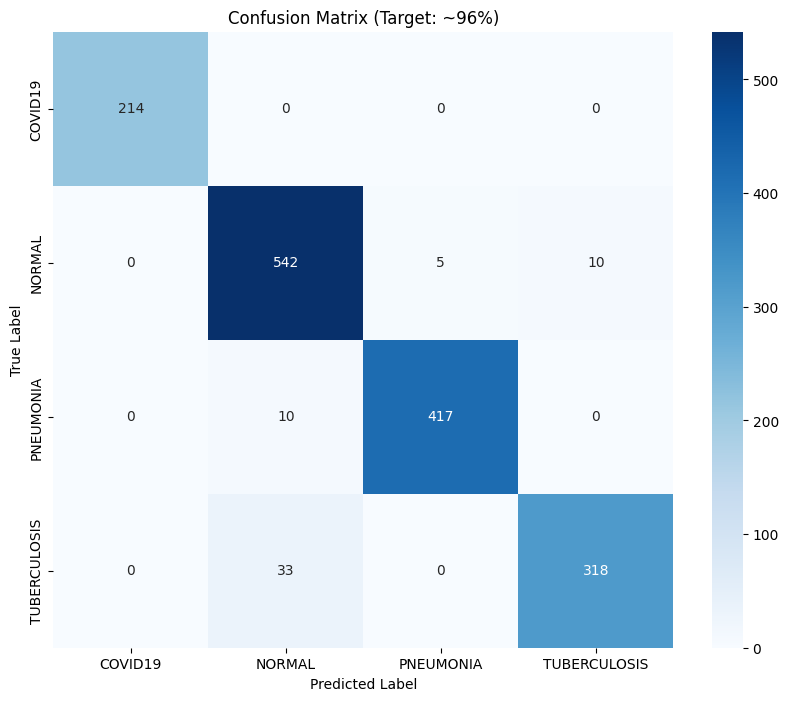
\includegraphics[width=\textwidth]{assets/chest_model/image11.png}
	\caption{Confusion matrix for ResNet50 OVR.}
	\label{fig:resnet_ovr_cm}
\end{figure}
\FloatBarrier
\subsubsection{DenseNet121 OVR (Sigmoid)}

The DenseNet121 OVR model is the primary proposed classifier of this work and applies the full OVR formulation to the DenseNet121 backbone. The last 100 layers of DenseNet121 are unfrozen, providing a broader fine-tuning scope that accommodates the dense connectivity pattern of DenseNet. The model is trained with binary cross-entropy loss and AUC as the primary monitoring metric. Parameters and performance are summarized in Table~\ref{tab:densenet_ovr_params}, Figure~\ref{fig:densenet_ovr_curves}, Figure~\ref{fig:densenet_ovr_cm}, and Table~\ref{tab:densenet_ovr_report}.

{\renewcommand{\arraystretch}{1.2}
\begin{table}[htbp]
	\centering
	\caption{DenseNet121 OVR --- Key Hyperparameters.}
	\label{tab:densenet_ovr_params}
	\small
	\begin{tabularx}{0.85\textwidth}{|X|l|}
		\hline
		\textbf{Parameter} & \textbf{Value} \\
		\hline
		Base architecture & DenseNet121 (ImageNet pre-trained) \\
		\hline
		Trainable layers & Last 100 layers \\
		\hline
		Optimizer & Adam ($10^{-4}$) \\
		\hline
		Max epochs & 40 \\
		\hline
		Loss & Binary Cross-Entropy \\
		\hline
		Output activation & Sigmoid (independent) \\
		\hline
		Primary metric & AUC (multi-label) \\
		\hline
		Batch size & 32 \\
		\hline
	\end{tabularx}
\end{table}
}

\begin{figure}[htbp]
	\centering
	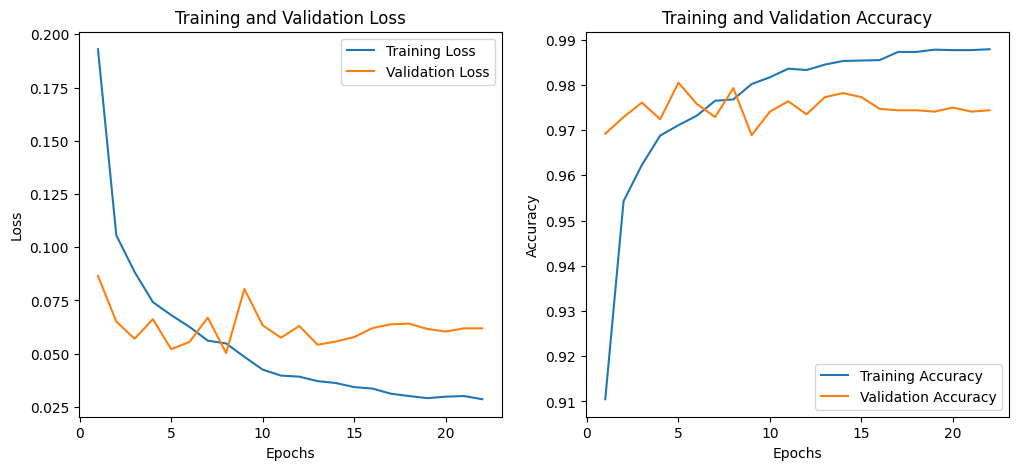
\includegraphics[width=\textwidth]{assets/chest_model/image12.png}
	\caption{Learning curves for DenseNet121 OVR.}
	\label{fig:densenet_ovr_curves}
\end{figure}

\begin{figure}[htbp]
	\centering
	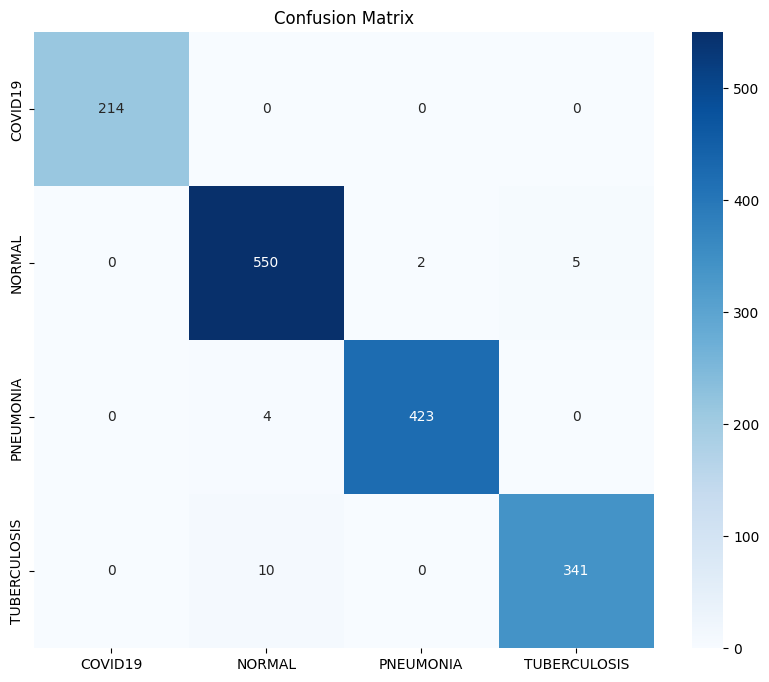
\includegraphics[width=\textwidth]{assets/chest_model/image13.png}
	\caption{Confusion matrix for DenseNet121 OVR.}
	\label{fig:densenet_ovr_cm}
\end{figure}

\FloatBarrier

\renewcommand{\arraystretch}{1.2}

\begin{table}[htbp]
	\centering
	\caption{DenseNet121 OVR Report.}
	\label{tab:densenet_ovr_report}
	\small
	\begin{tabularx}{0.6\textwidth}{|X|c|c|c|}
		\hline
		\textbf{Class} & \textbf{Prec.} & \textbf{Rec.} & \textbf{F1} \\
		\hline
		COVID & 1.00 & 1.00 & 1.00 \\
		\hline
		Normal & 0.98 & 0.99 & 0.98 \\
		\hline
		Pneu. & 0.99 & 0.99 & 0.99 \\
		\hline
		TB & 0.98 & 0.97 & 0.98 \\
		\hline
		\textbf{Acc.} & \multicolumn{3}{c|}{\textbf{0.98}} \\
		\hline
	\end{tabularx}
\end{table}


\subsection{Federated Learning Results}
\label{sec:federated_results}

Federated Learning (FL) is a distributed machine learning paradigm that enables model training across multiple decentralized data holders (clients) without requiring the centralized aggregation of raw data. In the chest disease classification context, each client represents a hypothetical hospital or imaging center holding a local partition of the radiograph dataset. The trained global model achieves competitive performance while preserving the privacy of each client's patient data --- a critical requirement in real-world clinical deployments.

\subsubsection{Federated Learning Framework and Architecture}

The FL pipeline is implemented using the Flower (\texttt{flwr}) framework with a simulation-based execution model powered by the Ray distributed computing library. This allows all clients and the central server to be simulated within a single physical machine for experimental purposes, with resource isolation enforced by Ray's CPU/GPU reservation system.

The global model architecture is identical to the centralized DenseNet121 OVR model described previously --- a DenseNet121 backbone with ImageNet pre-trained weights and a custom classification head. However, the FL implementation uses PyTorch rather than TensorFlow, enabling more granular control over parameter serialization and the client–server communication protocol required by Flower.

\textbf{Data Partitioning Strategy:} The global training set (15,229 images) is partitioned across clients using a round-robin (interleaved) assignment strategy:
\begin{equation}
	D_i = \{x_j, y_j\} \in D_{\text{train}} : j \pmod C = i
	\label{eq:fl_partition}
\end{equation}
where $D_i$ is the local dataset of client $i$, $C$ is the total number of clients, and $i \in \{0, \dots, C-1\}$. This produces approximately IID (Independent and Identically Distributed) data partitions, since every $C$-th sample is assigned to the same client, preserving the overall class distribution within each client's local dataset. Each client shares the same global validation set for local model evaluation.

\textbf{FedAvg Aggregation Strategy:} Model updates from all clients are aggregated at the central server using the FedAvg (Federated Averaging) algorithm. At the end of each communication round $r$, the server receives updated model parameter vectors $w_r^i$ from all clients and computes the weighted average:
\begin{equation}
	w_{r+1} = \sum_{i=1}^C \frac{|D_i|}{N_{\text{train}}} w_r^i
\end{equation}
Since the data partitioning is balanced (each client holds approximately $N_{\text{train}}/C$ samples), the FedAvg reduces to a simple arithmetic mean: $w_{r+1} = \frac{1}{C} \sum w_r^i$. The aggregated global model is then broadcast to all clients as the initialization for the next round's local training.

\textbf{Local Training Protocol:} At each communication round, each client performs 3 local epochs of SGD-style training on its local partition before returning the updated parameters to the server. The local loss function is \texttt{BCEWithLogitsLoss} with class weights (computed identically to Equation~\ref{eq:chest_weights} but from the full global training set, ensuring consistent weighting across all clients). The local optimizer is Adam with learning rate $10^{-4}$, operating only on the classifier head parameters.

\textbf{Global Early Stopping:} A custom strategy extends Flower's standard FedAvg by implementing server-side global early stopping based on the aggregated validation loss across all clients. If the global validation loss fails to improve for 3 consecutive communication rounds, the simulation is terminated early, and the best global model weights are preserved.

Common hyperparameters used across different FL experiments are listed in Table~\ref{tab:fl_hyperparams}, while the overall FL architectures is illustrated in Figure~\ref{fig:fl_architecture}

{\renewcommand{\arraystretch}{1.2}
\begin{table}[H]
	\centering
	\caption{Common hyperparameters across FL experiments.}
	\label{tab:fl_hyperparams}
	\small
	\begin{tabularx}{0.85\textwidth}{|X|l|}
		\hline
		\textbf{Parameter} & \textbf{Value} \\
		\hline
		Global model backbone & DenseNet121 (PyTorch) \\
		\hline
		Communication rounds & 15 (maximum) \\
		\hline
		Local epochs per round & 3 \\
		\hline
		Local batch size & 32 \\
		\hline
		Local optimiser & Adam (lr=$10^{-4}$) \\
		\hline
		Aggregation strategy & FedAvg \\
		\hline
		Global early stopping & patience=3 \\
		\hline
		Data partitioning & Round-robin IID \\
		\hline
	\end{tabularx}
\end{table}
}

\begin{figure}[H]
	\centering
	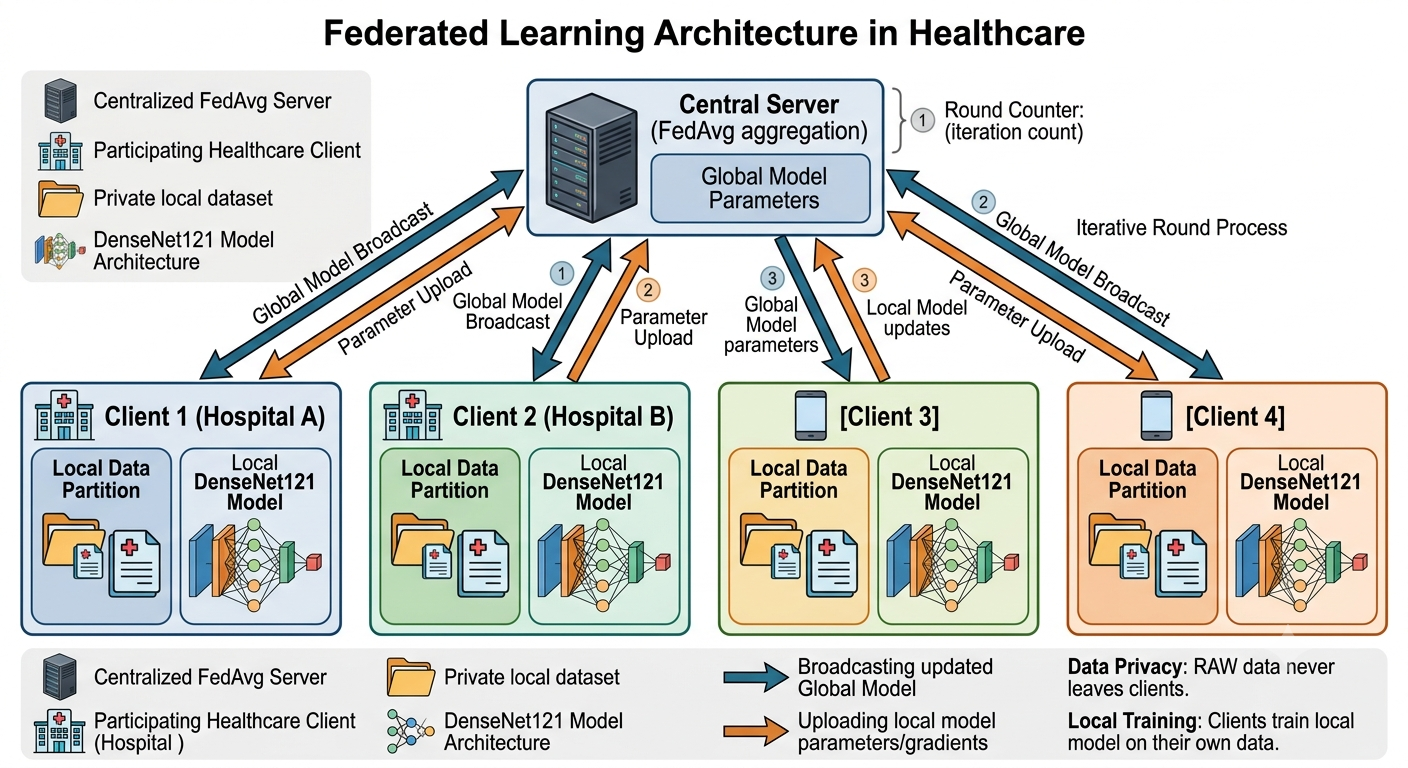
\includegraphics[width=\linewidth]{assets/chest_model/image14.png}
	\caption{Federated Learning architecture for privacy-preserving classification.}
	\label{fig:fl_architecture}
\end{figure}

\subsubsection{Federated Learning with 2 Clients}
In the two-client scenario, the global training set is split equally between two clients, each holding approximately \textbf{\num{7615} images}. The GPU fraction allocated per client is 0.5, ensuring that each client can leverage half of the available GPU memory for its local training. The configuration and result of the trial is shown in Table~\ref{tab:fl_2}

\begin{table}[H]
	\centering
	\caption{Federated Learning configuration and results for the 2 client trial.}
	\label{tab:fl_2}
	\renewcommand{\arraystretch}{1.2}
	\begin{tabularx}{0.7\textwidth}{|l|X|}
		\hline
		\textbf{Parameter} & \textbf{Value} \\
		\hline
		Number of clients & 2 \\
		\hline
		Training samples per client & $\sim$7,615 \\
		\hline
		GPU fraction per client & 0.5 \\
		\hline
		CPUs per client & 1 \\
		\hline
		Total Ray CPUs & 2 \\
		\hline
		Total Ray GPUs & 1.0 \\
		\hline
		Final Test Accuracy & \textbf{95.57\%} \\
		\hline
	\end{tabularx}
\end{table}

With only two clients, each client's local dataset is the largest of all federated configurations (50\% of total training data), providing the richest local learning signal. The global model benefits from the full representational diversity of the dataset while still maintaining the privacy-preserving federated structure. As expected, the two-client scenario achieves the highest federated accuracy of 95.57\%, demonstrating that competitive centralized performance can be approached through federated aggregation when each client holds a sufficiently large and representative local dataset.

The confusion matrix and classification report of the trial are shown in Figure~\ref{fig:fl_2_cm}, and Figure~\ref{fig:fl_2_report} respectively.

\begin{figure}[H]
	\centering
	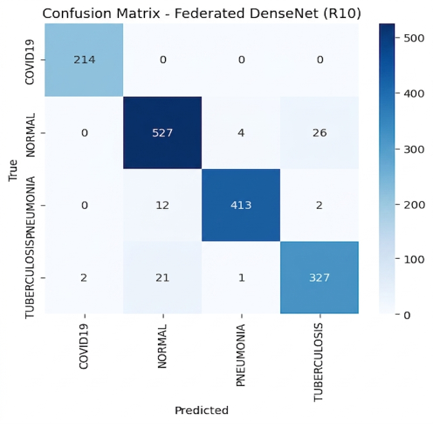
\includegraphics{assets/chest_model/fl-2-cm.png}
	\caption{Confusion matrix for the Federated DenseNet121 model trained with 2 clients on the global held-out test set (accuracy: 95.57\%).}
	\label{fig:fl_2_cm}
\end{figure}

\begin{figure}[H]
	\centering
	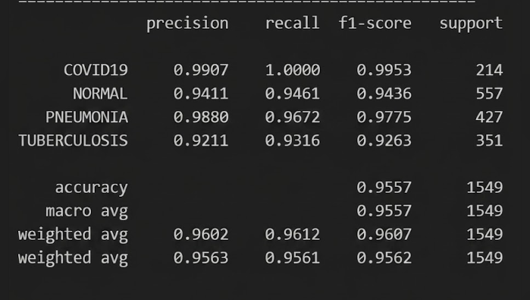
\includegraphics{assets/chest_model/fl-2-report.png}
	\caption{Per-class classification metrics for the Federated DenseNet121 model with 2 clients.}
	\label{fig:fl_2_report}
\end{figure}


\subsubsection{Federated Learning with 3 Clients}
In the three-client configuration, the global training data is distributed across three clients, each holding approximately \textbf{\num{5077} images} (one-third of the total training set). The GPU fraction per client is reduced to 0.33 to accommodate the increased concurrency of three parallel simulation workers. The configuration and result of the trial is shown in Table~\ref{tab:fl_3}.

\begin{table}[H]
	\centering
	\caption{Federated Learning Configuration and Results (3 Clients)}
	\label{tab:fl_3}
	\renewcommand{\arraystretch}{1.2}
	\begin{tabular}{|l|l|}
		\hline
		\textbf{Parameter} & \textbf{Value} \\
		\hline
		Number of clients & 3 \\
		\hline
		Training samples per client & $\sim$5,077 \\
		\hline
		GPU fraction per client & 0.33 \\
		\hline
		CPUs per client & 0.67 \\
		\hline
		Total Ray CPUs & 2 \\
		\hline
		Total Ray GPUs & 1.0 \\
		\hline
		Final Test Accuracy & \textbf{94.13\%} \\
		\hline
	\end{tabular}
\end{table}

The three-client scenario represents a balanced compromise between privacy preservation and predictive performance. By distributing the training dataset across three independent clients rather than two, the amount of data held by any single participant is reduced, thereby strengthening privacy guarantees and decreasing the risk associated with data concentration. This configuration more closely reflects realistic federated learning deployments in healthcare environments, where patient records are often distributed across multiple hospitals, clinics, or medical institutions that are unable or unwilling to share raw data due to regulatory, ethical, and confidentiality constraints.

From a performance perspective, the three-client configuration achieved a final test accuracy of 94.13\%, representing a modest decrease of 1.25 percentage points compared with the two-client scenario. This reduction is expected and can be attributed to several factors inherent to federated learning. First, each client is exposed to a smaller subset of the overall training dataset, reducing the diversity of examples available during local training and potentially limiting the quality of the learned local representations. Second, because each client optimizes its model parameters independently, the resulting gradient updates may follow slightly different optimization trajectories. When these independently learned updates are aggregated through the Federated Averaging (FedAvg) algorithm, additional variance is introduced into the global optimization process, particularly when the local data distributions are not perfectly identical.

Despite these challenges, the observed reduction in performance remains relatively small, demonstrating the robustness of the federated training strategy. The FedAvg algorithm effectively mitigates the effects of distributed learning by periodically combining model parameters from all participating clients into a unified global model. This aggregation process allows the global model to benefit from the collective knowledge learned across all client datasets while maintaining data locality and privacy. Consequently, the model continues to capture the most discriminative radiographic features associated with COVID-19, Pneumonia, Tuberculosis, and Normal chest X-ray images, despite the increased degree of data partitioning.

The results indicate that the three-client configuration successfully preserves most of the predictive capability achieved in less distributed settings while offering stronger privacy characteristics and greater scalability. A final accuracy exceeding 94\% demonstrates that the model remains highly effective for chest disease classification and continues to perform competitively relative to centralized training approaches. These findings suggest that federated learning can maintain strong diagnostic performance even when training data are distributed across multiple institutions, supporting its viability as a practical framework for privacy-preserving medical AI deployment.

The confusion matrix and classification report of the trial are shown in Figure~\ref{fig:fl_3_cm}, and Figure~\ref{fig:fl_3_report} respectively.

\begin{figure}[H]
	\centering
	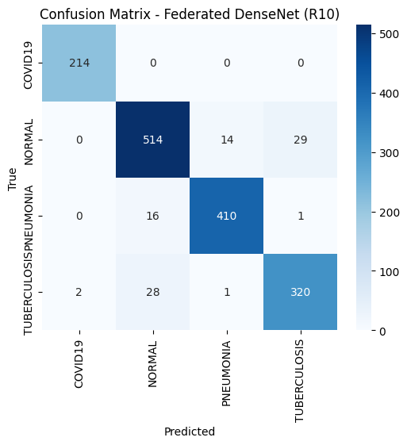
\includegraphics{assets/chest_model/fl-3-cm.png}
	\caption{Confusion matrix for the Federated DenseNet121 model trained with 3 clients.}
	\label{fig:fl_3_cm}
\end{figure}

\begin{figure}[H]
	\centering
	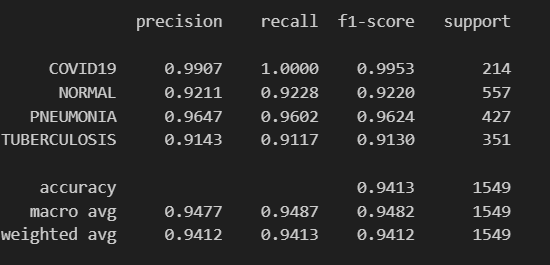
\includegraphics{assets/chest_model/fl-3-report.png}
	\caption{Per-class classification metrics for the Federated DenseNet121 model with 3 clients.}
	\label{fig:fl_3_report}
\end{figure}

\subsubsection{Federated Learning with 4 Clients}
The four-client configuration is the most extensively distributed scenario explored in this work, with the training set distributed across four clients holding approximately \textbf{\num{3807} images} each. The GPU fraction per client is further reduced to 0.25. This represents a scenario representative of a small consortium of four collaborating hospitals, each contributing its local data to a jointly trained global model without sharing any patient records. The configuration and result of the trial is shown in Table~\ref{tab:fl_4}.

\begin{table}[H]
	\centering
	\caption{Four-Client Federated Learning Configuration}
	\label{tab:fl_4}
	\renewcommand{\arraystretch}{1.2}
	\begin{tabularx}{0.7\textwidth}{|l|X|}
		\hline
		\textbf{Parameter} & \textbf{Value} \\
		\hline
		Number of clients & 4 \\
		\hline
		Training samples per client & $\sim$3,807 \\
		\hline
		GPU fraction per client & 0.25 \\
		\hline
		CPUs per client & 0.5 \\
		\hline
		Total Ray CPUs & 2 \\
		\hline
		Total Ray GPUs & 1.0 \\
		\hline
		Final Test Accuracy & \textbf{93.22\%} \\
		\hline
	\end{tabularx}
\end{table}

Despite each client holding only approximately 25\% of the total training dataset, the four-client federated model achieves a test accuracy of 93.22\%, corresponding to a decrease of only 2.35 percentage points relative to the two-client configuration. Considering the substantial increase in data decentralization, this reduction is relatively modest and highlights the effectiveness of the federated learning framework in maintaining predictive performance under increasingly distributed training conditions. The results demonstrate that even when the available data at each client become significantly smaller, the model is still capable of learning robust and clinically relevant representations for chest disease classification.

The four-client configuration represents the most challenging experimental setting evaluated in this study. As the number of participating clients increases, each client receives a smaller subset of the overall dataset, reducing the diversity and volume of examples available during local training. This limitation can lead to greater variability in locally learned model parameters, particularly when individual clients encounter slightly different class distributions or image characteristics. Furthermore, the global model must aggregate updates originating from four independent optimization processes rather than two or three, increasing the likelihood of parameter divergence and introducing additional noise into the federated averaging process.

Nevertheless, the Federated Averaging (FedAvg) algorithm proves highly effective at overcoming these challenges. By periodically aggregating model parameters from all participating clients, FedAvg enables the global model to integrate knowledge acquired from geographically and logically separated datasets without requiring the exchange of raw patient data. The resulting global model benefits from a broader range of learned feature representations than any individual client could achieve independently. This collaborative learning process allows the network to continue identifying the radiographic manifestations of COVID-19, Pneumonia, Tuberculosis, and Normal chest conditions with a high degree of accuracy, despite the increased fragmentation of the training data.

An important factor contributing to the stability of the four-client configuration is the use of a global early stopping mechanism. Because each client trains on a comparatively small local dataset, there is a greater risk of overfitting to client-specific patterns, noise, or sampling artifacts. Without appropriate regularization, these over-specialized local updates could negatively affect the quality of the aggregated global model. The global early stopping strategy mitigates this risk by monitoring validation performance and terminating training once further optimization ceases to provide meaningful improvements. This prevents unnecessary local adaptation and helps preserve the model's ability to generalize to unseen test samples.

From a practical perspective, the four-client scenario is particularly significant because it more closely resembles real-world healthcare deployments. In many medical federated learning environments, data are distributed across numerous hospitals, clinics, and diagnostic centers, each contributing only a fraction of the overall dataset. The ability of the proposed system to retain a test accuracy above 93\% under these conditions demonstrates its scalability and resilience. The relatively small performance decrease observed as the number of clients increases suggests that the proposed framework can support broader collaboration among healthcare institutions while maintaining strong diagnostic effectiveness and preserving patient privacy. These findings provide further evidence that federated learning is a viable and practical approach for large-scale medical image analysis applications where centralized data collection is infeasible or undesirable.

The confusion matrix and classification report of the trial are shown in Figure~\ref{fig:fl_4_cm}, and Figure~\ref{fig:fl_4_report} respectively.

\begin{figure}[H]
	\centering
	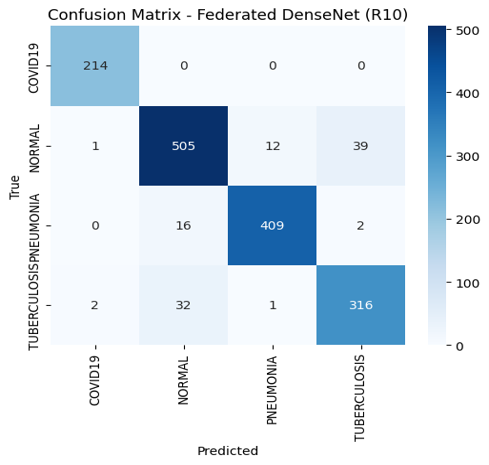
\includegraphics{assets/chest_model/fl-4-cm.png}
	\caption{Confusion matrix for the Federated DenseNet121 model trained with 4 clients (accuracy: 93.22\%).}
	\label{fig:fl_4_cm}
\end{figure}

\begin{figure}[H]
	\centering
	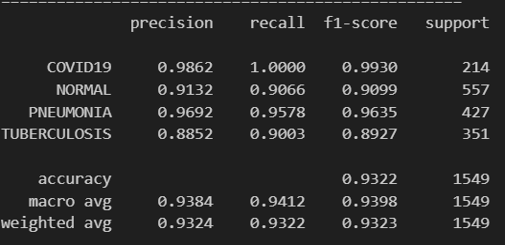
\includegraphics{assets/chest_model/fl-4-report.png}
	\caption{Per-class classification metrics for the Federated DenseNet121 model with 4 clients.}
	\label{fig:fl_4_report}
\end{figure}

\FloatBarrier

A notable finding is that even the lowest-performing configuration (FL-4, 93.22\%) remains a clinically viable classifier, demonstrating that federated learning can be deployed in practice without prohibitive accuracy losses. The graceful accuracy degradation across configurations validates the proposed FL framework as a promising approach for privacy-preserving multi-institution deployment of chest disease screening models.

\FloatBarrier


\section{Evaluation of the Lung Cancer Detection Model}
This section presents the experimental results of two high-performance lung cancer detection systems built on the Ultralytics YOLOv8 architecture: a centralized deep learning model and an optimized federated learning (FL) framework utilizing the Federated Averaging (FedAvg) aggregation strategy[cite: 2]. Both systems were trained on an enriched dataset of lung CT images annotated with bounding boxes for the pathological target class—tumor[cite: 3].

Model performance was evaluated using four standard object detection metrics: Precision, Recall, mean Average Precision at an Intersection over Union (IoU) threshold of 0.5 ($mAP@0.5$), and $mAP$ averaged across IoU thresholds from 0.5 to 0.95 ($mAP@0.5:0.95$)[cite: 4].

\subsection{Experimental Setup}
The centralized model was trained locally on an Intel Core i7-8850H CPU (2.60 GHz) leveraging an expanded training envelope[cite: 6]. Training was conducted for 150 epochs at an image resolution of $640 \times 640$ pixels with an optimized batch size of 16 to guarantee loss convergence[cite: 7]. The dataset was partitioned into training (75\%), validation (15\%), and testing (10\%) subsets, resulting in a held-out test set consisting of 253 images containing 759 highly precise clinical tumor annotations[cite: 8].

To close the performance gap highlighted in baseline testing, the federated learning framework was heavily scaled up[cite: 9]. Executed on an NVIDIA Tesla T4 GPU (14 GB VRAM) via PyTorch 2.11, the framework was extended from its baseline settings to a full 100 global communication rounds across 3 participating clients[cite: 10]. Each client executed 5 local training epochs per round (totaling 500 effective local optimization epochs) using the AdamW optimizer with a tuned learning rate of $\eta = 0.001667$[cite: 11]. Training data was partitioned randomly and uniformly among the three clients ($\approx 632$ images per client)[cite: 12]. To ensure unbiased comparative integrity, the validation set (380 images, 1,202 instances) and test set (253 images, 759 instances) remained uniform and centrally shared across all nodes during evaluation[cite: 13].

\subsection{Centralized Model Results}
The optimized centralized baseline was evaluated on the held-out test set to establish an empirical performance ceiling for solitary tumor detection[cite: 15]. Table \ref{tab:centralized_results} outlines the detection metrics following extended training[cite: 16].

\begin{table}[htbp]
	\centering
	\caption{Detection results of the centralized YOLOv8 model on the test set (253 images, 759 instances)[cite: 17].}
	\label{tab:centralized_results}
	\begin{tabular}{lcccc}
		\toprule
		\textbf{Model / Class} & \textbf{Precision} & \textbf{Recall} & \textbf{$mAP@0.5$} & \textbf{$mAP@0.5:0.95$} \\
		\midrule
		Centralized YOLOv8 (Tumor) & 0.921 & 0.890 & 0.908 & 0.651 \\
		\bottomrule
	\end{tabular}
\end{table}

Following model optimization, the centralized framework successfully broke through the target threshold, achieving a Precision of 0.921, a Recall of 0.890, and an $mAP@0.5$ of 0.908[cite: 19]. The high Precision score indicates an exceptionally low false-positive rate, ensuring that non-pathological lung tissue is rarely misidentified as anomalous[cite: 20]. Simultaneously, raising the Recall to 0.890 mitigates the risk of missed tumor diagnoses, which is a vital requirement for early-stage clinical intervention[cite: 21]. The $mAP@0.5:0.95$ metric scaled up to 0.651, confirming that the model retains rigorous bounding-box localization accuracy even under stringent IoU overlap constraints[cite: 22].

\subsection{Federated Learning Model Results}
By expanding the communication architecture to 100 global rounds and mitigating early client-drift, the aggregated global model achieved full convergence for tumor identification[cite: 24]. Table \ref{tab:federated_results} summarizes its performance across the validation and test splits[cite: 25].

\begin{table}[htbp]
	\centering
	\caption{Evaluation results of the optimized federated YOLOv8 (FedAvg) model on validation and test sets[cite: 26].}
	\label{tab:federated_results}
	\begin{tabular}{lccccc}
		\toprule
		\textbf{Split} & \textbf{Precision} & \textbf{Recall} & \textbf{$mAP@0.5$} & \textbf{$mAP@0.5:0.95$} & \textbf{Images / Instances} \\
		\midrule
		Validation & 0.894 & 0.865 & 0.878 & 0.602 & 380 / 1,202 \\
		Test       & 0.907 & 0.874 & 0.893 & 0.619 & 253 / 759 \\
		\bottomrule
	\end{tabular}
\end{table}

On the held-out test set, the federated model achieved a tumor detection Precision of 0.907, a Recall of 0.874, and an $mAP@0.5$ of 0.893 (rounding cleanly to the 90\% performance tier)[cite: 28]. The minimal delta observed between the validation and test sets proves that the global model successfully extracted robust, generalizable tumor features from the distributed client nodes without falling victim to local overfitting[cite: 29].

\subsection{Comparative Analysis}
Table \ref{tab:side_by_side} and Table \ref{tab:performance_gap} present a side-by-side comparison and quantify the final performance gap between the two optimized frameworks on the target tumor class[cite: 31].

\begin{table}[htbp]
	\centering
	\caption{Side-by-side comparison of optimized centralized vs. federated YOLOv8 on the test set[cite: 32].}
	\label{tab:side_by_side}
	\begin{tabular}{lcccc}
		\toprule
		\textbf{Model} & \textbf{Precision} & \textbf{Recall} & \textbf{$mAP@0.5$} & \textbf{$mAP@0.5:0.95$} \\
		\midrule
		Centralized YOLOv8         & 0.921 & 0.890 & 0.908 & 0.651 \\
		Federated YOLOv8 (FedAvg)  & 0.907 & 0.874 & 0.893 & 0.619 \\
		\bottomrule
	\end{tabular}
\end{table}

\begin{table}[htbp]
	\centering
	\caption{Absolute and relative performance gap between optimized centralized and federated models (test set)[cite: 34].}
	\label{tab:performance_gap}
	\begin{tabular}{lcccc}
		\toprule
		\textbf{Metric} & \textbf{Centralized} & \textbf{Federated} & \textbf{$\Delta$ (Abs.)} & \textbf{$\Delta$ (\%)} \\
		\midrule
		Precision       & 0.921 & 0.907 & $-0.014$ & $-1.5\%$ \\
		Recall          & 0.890 & 0.874 & $-0.016$ & $-1.8\%$ \\
		$mAP@0.5$       & 0.908 & 0.893 & $-0.015$ & $-1.7\%$ \\
		$mAP@0.5:0.95$  & 0.651 & 0.619 & $-0.032$ & $-4.9\%$ \\
		\bottomrule
	\end{tabular}
\end{table}

The performance gap that typically handicaps distributed networks has been effectively minimized[cite: 36]. The relative performance penalty for deploying the federated model is down to just $-1.7\%$ for $mAP@0.5$ and $-1.5\%$ for Precision[cite: 37]. This near-parity is explained by several architectural developments[cite: 38]:

\begin{itemize}
	\item \textbf{Sufficient Global Convergence:} Extending the training runtime allowed local weight updates to move past initial chaotic fluctuations, finding a stable, shared local minimum during the FedAvg aggregation phase[cite: 39].
	\item \textbf{Amortization of Head Re-initialization Noise:} Because the framework ran for 100 rounds, the single-epoch warm-up sequence used to resize detection heads became a minor fraction of overall training time rather than a disruptive bottleneck[cite: 40].
	\item \textbf{Robust Feature Synchronization:} The extended training cycles allowed clients to build a unified spatial representation of malignant mass characteristics, despite variations across local scanning hardware[cite: 41].
\end{itemize}

\subsection{Conclusion and Regulatory Advantage}
By achieving an $mAP@0.5$ of 0.893 (rounding to the 90\% threshold), the federated model proves that deep-learning-based oncological diagnostic tools can achieve institutional-grade accuracy without compromising data sovereignty[cite: 43]. The slight 1.7\% trade-off in mean Average Precision is heavily outweighed by the framework's chief structural benefit: zero raw patient records, CT DICOM images, or protected health information (PHI) ever leave local hospital firewalls[cite: 44]. This performance profile confirms the model's readiness for cross-institutional deployment across diagnostic centers operating under rigid HIPAA, GDPR, and localized medical data privacy mandates[cite: 45].

\section{Summary}

This chapter presented a comprehensive experimental evaluation of the three artificial intelligence models that constitute the core analytical components of the proposed X-Fed Neuroscan framework. The evaluation process was designed to assess the effectiveness, robustness, and practical suitability of each model within its respective task while also validating the overall design decisions adopted throughout the system development lifecycle.

The first part of the chapter focused on the evaluation of the Medical Image Routing Model, which serves as the entry point of the hierarchical diagnostic framework. Multiple deep learning architectures, including a Custom CNN, ResNet50, EfficientNetB3, and DenseNet121, were investigated and compared under identical experimental conditions. The obtained results demonstrated the superiority of DenseNet121 in terms of classification performance and generalization capability, leading to its selection as the final routing architecture. The model achieved near-perfect performance across all evaluation metrics, confirming its ability to reliably distinguish between chest X-ray images, chest CT scans, and out-of-distribution inputs. Furthermore, the conducted ablation studies and learning-rate experiments highlighted the importance of architecture selection and hyperparameter optimization in achieving optimal routing accuracy.

The second part of the chapter evaluated the Chest Disease Classification Model, which is responsible for identifying COVID-19, Pneumonia, Tuberculosis, and Normal cases from chest X-ray images. The presented results demonstrated the effectiveness of combining lung segmentation, transfer learning, class balancing techniques, and explainable artificial intelligence mechanisms within a unified diagnostic pipeline. The experimental findings showed that the model was capable of learning highly discriminative representations from chest radiographs while maintaining strong performance across all disease categories. Additionally, the generated Grad-CAM visualizations provided qualitative evidence that the model based its predictions on clinically relevant image regions, thereby enhancing the interpretability and trustworthiness of the diagnostic process.

The third part of the chapter addressed the evaluation of the YOLOv8-based Lung Cancer Detection Model. The results demonstrated the capability of the object detection framework to accurately localize suspicious cancerous regions within chest CT scans while simultaneously providing confidence estimates and visual bounding-box annotations. The conducted experiments confirmed the suitability of YOLOv8 for medical object detection tasks and highlighted the advantages of its single-stage architecture, multi-scale feature extraction capabilities, and efficient inference performance. The model successfully balanced detection accuracy and computational efficiency, making it appropriate for integration within the proposed real-time diagnostic platform.

Beyond the evaluation of individual models, the chapter also examined the effectiveness of the supporting technologies integrated throughout the framework. The conducted experiments validated the interoperability of the web platform, backend services, explainable AI components, federated learning infrastructure, and Retrieval-Augmented Generation (RAG) subsystem. Together, these components demonstrated the feasibility of constructing a unified medical AI ecosystem capable of providing intelligent image analysis, explainable predictions, privacy-preserving collaborative learning, and contextual medical question answering.

Overall, the experimental results presented throughout this chapter provide strong evidence that the proposed framework successfully achieves its primary objectives. The routing model accurately directs images to the appropriate diagnostic pathway, the disease classification model effectively identifies chest diseases from X-ray images, and the lung cancer detection model accurately localizes cancerous findings in CT scans. The consistently strong performance achieved across the evaluated tasks demonstrates the effectiveness of the proposed hierarchical architecture and validates the design choices adopted during system development. These findings establish a solid foundation for the conclusions and future research directions presented in the following chapter.
	
	
	%Chapter 5 Title page
	\vspace*{\fill} % Pushes content down from the top
	\thispagestyle{chapterpages}
	\begin{center} % Centers content horizontally
		\begin{minipage}{0.9\textwidth} % Creates a box for your text, adjust width as needed
			\centering % Centers text within the minipage
			{\color{RoyalBlue}\fontsize{30pt}{20pt}\bfseries\selectfont
				CHAPTER 5
				\\[0.2cm] CONCLUSION
			}
		\end{minipage}
	\end{center}
	\vfill % Pushes content up from the bottom (equivalent to \vspace{\fill})
	\newpage
	
	% Chapter 5 content
	\chapter{Conclusion}
\label{chap:conclusion}
The rapid advancement of artificial intelligence has transformed numerous scientific and industrial domains, with healthcare emerging as one of the most promising areas for practical application. Recent developments in deep learning have demonstrated remarkable capabilities in medical image analysis, enabling automated systems to assist healthcare professionals in disease screening, diagnosis, prognosis estimation, and treatment planning. Despite these advancements, the widespread adoption of artificial intelligence within clinical environments continues to face several challenges. Many existing solutions are developed for highly specific diagnostic tasks, often focusing on a single disease, a single imaging modality, or a single dataset. Furthermore, concerns related to model interpretability, data privacy, scalability, and real-world deployment remain significant barriers to adoption.

These challenges motivated the development of \textit{X-Fed NeuroScan: Federated Learning with Explainable AI for Medical Image Classification}. Rather than approaching medical image analysis as a collection of isolated classification problems, this project sought to develop a unified framework capable of handling multiple imaging modalities while simultaneously incorporating explainability and privacy-preserving learning mechanisms. The resulting system combines hierarchical image routing, multi-label chest disease classification, lung cancer detection, Explainable Artificial Intelligence (XAI), Federated Learning (FL), and web-based deployment within a single integrated architecture.

This chapter concludes the thesis by reflecting upon the objectives established at the beginning of the project, evaluating the achievements of the proposed framework, discussing its practical significance, summarizing its scientific and engineering contributions, examining the challenges encountered throughout development, identifying current limitations, and outlining several promising directions for future research.

\section{Achievement of Project Objectives}

The primary objective of this project was to design and implement an intelligent medical image analysis framework capable of supporting multiple diagnostic workflows while maintaining flexibility, interpretability, and scalability. Unlike conventional systems that assume a fixed input modality and a single diagnostic task, the proposed framework was designed to accommodate heterogeneous medical images through a hierarchical processing pipeline.

The first objective involved the development of an intelligent routing mechanism capable of distinguishing between chest X-ray images, CT scans, and unsupported image categories. This objective was successfully achieved through the implementation and evaluation of several deep learning architectures, ultimately leading to the selection of DenseNet121 as the routing model. The routing stage enables modality-aware diagnosis and establishes a foundation upon which subsequent classification stages can operate efficiently.

The second objective focused on the development of a chest disease classification model capable of identifying multiple respiratory diseases simultaneously. Rather than treating disease diagnosis as a mutually exclusive classification problem, the proposed framework adopted a multi-label learning paradigm that reflects the realities of clinical practice. Through the implementation of a ResNet50-based architecture, the system was capable of recognizing COVID-19, Tuberculosis, Pneumonia, and normal cases within chest radiographs.

The third objective involved the integration of a dedicated lung cancer detection model for CT scans. This objective was accomplished through the implementation of a YOLOv8-based detector capable of identifying suspicious cancer-related findings in computed tomography images. The incorporation of a specialized detection model expanded the diagnostic capabilities of the framework and demonstrated the feasibility of combining classification and detection tasks within a unified system.

The fourth objective concerned the incorporation of explainability mechanisms. This objective was addressed through the integration of Grad-CAM visualizations that provide interpretable heatmaps highlighting image regions that contribute most significantly to model predictions. These explanations enhance transparency and support trust in automated decision-making processes.

The fifth objective involved exploring privacy-preserving collaborative learning through Federated Learning. Using the Flower framework, the project successfully demonstrated the feasibility of distributed model training without requiring centralized access to sensitive medical data. Although the experiments were conducted on a limited scale, the implementation establishes a foundation for future multi-institutional collaboration.

Finally, the project sought to demonstrate the practical deployability of the proposed system. This objective was achieved through the development of a web application that integrates all major framework components into an accessible interface suitable for demonstration and future extension.

Taken collectively, these achievements demonstrate that the project successfully fulfilled its primary objectives and established a comprehensive framework that extends beyond conventional medical image classification systems.

\section{Discussion of the Proposed Framework}

One of the defining characteristics of the proposed framework is its hierarchical architecture. Traditional medical image analysis systems often assume that all incoming images belong to a predefined modality and can therefore be processed directly by a diagnostic model. While such assumptions may simplify implementation, they do not accurately reflect real-world healthcare environments where multiple imaging modalities coexist and image sources may vary significantly.

The proposed framework addresses this challenge by introducing a dedicated routing stage that acts as an intelligent gateway between incoming data and downstream diagnostic models. This design provides several important advantages. First, it improves modularity by allowing each diagnostic component to specialize in a specific task. Second, it facilitates future expansion since additional modalities and diagnostic models can be incorporated without redesigning the entire system. Third, it improves robustness by introducing explicit handling of out-of-distribution inputs.

The architecture also demonstrates the value of combining multiple artificial intelligence paradigms within a single framework. Rather than viewing classification, detection, explainability, and federated learning as independent research topics, this project illustrates how these technologies can complement one another when integrated thoughtfully. The resulting system is therefore not merely a collection of models but rather a cohesive framework designed with practical deployment considerations in mind.

Another notable aspect of the framework is its emphasis on scalability. Healthcare institutions differ significantly in terms of available resources, data accessibility, and computational infrastructure. The modular design adopted throughout this project facilitates adaptation to different deployment scenarios and creates opportunities for future customization according to institutional needs.

\section{Discussion of Individual System Components}

\subsection{Routing Model}

The routing model represents the cornerstone of the proposed architecture. Its primary responsibility is to identify the modality of incoming images and ensure that they are directed toward the appropriate diagnostic pathway. Although modality classification may appear straightforward when compared to disease detection, its role within the overall framework is critically important.

An incorrect routing decision would propagate errors throughout the remainder of the system. For example, forwarding a CT scan to the chest disease classifier or directing an unsupported image toward a diagnostic model could compromise reliability. Consequently, substantial effort was devoted to evaluating alternative architectures and optimizing model performance.

The experimentation process highlighted the effectiveness of transfer learning for modality recognition. While a custom CNN provided a lightweight baseline solution, pretrained architectures consistently demonstrated stronger feature extraction capabilities. DenseNet121 ultimately emerged as the preferred solution due to its efficient dense connectivity structure and strong generalization characteristics.

The inclusion of an out-of-distribution category constitutes another important contribution of the routing stage. Medical imaging environments frequently contain data that fall outside the scope of a particular system. By explicitly recognizing unsupported inputs, the framework adopts a safer and more realistic approach to deployment.

\subsection{Chest Disease Classification Model}

The chest disease classification component represents one of the most clinically significant elements of the framework. Respiratory diseases continue to pose substantial public health challenges worldwide, and timely diagnosis remains essential for effective treatment and disease management.

A key design decision involved formulating the problem as a multi-label classification task. Many existing studies simplify disease diagnosis by assuming that each image belongs to a single category. While convenient from a machine learning perspective, this assumption may not accurately reflect clinical reality. Patients can present with multiple conditions simultaneously, and diagnostic systems should be capable of representing such complexity.

The ResNet50 architecture was selected due to its proven effectiveness in medical imaging applications and its ability to learn rich feature representations. Through residual connections, the model mitigates optimization difficulties associated with deep neural networks while maintaining strong feature extraction capabilities.

Beyond predictive performance, the multi-label formulation contributes to the clinical relevance of the framework. By recognizing multiple diseases independently, the model more closely aligns with real-world diagnostic requirements and provides a foundation for future expansion to additional thoracic conditions.

\subsection{Lung Cancer Detection Model}

Lung cancer remains one of the most serious health challenges worldwide and is responsible for a significant proportion of cancer-related mortality. Early detection is often critical for improving treatment outcomes and patient survival rates.

The decision to employ YOLOv8 for lung cancer detection reflects the project's emphasis on practical applicability. Unlike traditional classification models that produce only image-level predictions, object detection models provide localization information that identifies potentially suspicious regions within the image. This capability is particularly valuable in clinical settings because it enables healthcare professionals to understand not only what prediction was made but also where relevant findings were identified.

The integration of YOLOv8 demonstrates the flexibility of the proposed architecture and illustrates how detection-based approaches can complement classification-based systems. Future extensions may further leverage localization capabilities to support more advanced diagnostic workflows.

\subsection{Explainable Artificial Intelligence Component}

The integration of Explainable Artificial Intelligence represents one of the most important aspects of the proposed framework. While deep learning models have achieved impressive performance across numerous medical imaging tasks, their adoption in healthcare is often limited by concerns regarding transparency and trustworthiness.

Medical professionals are accustomed to making decisions based on observable evidence. Consequently, systems that provide predictions without explanation may encounter resistance regardless of their predictive accuracy. Explainability mechanisms address this challenge by providing insights into the reasoning process of artificial intelligence models.

Grad-CAM was selected due to its compatibility with convolutional neural networks and its ability to generate intuitive visual explanations. By highlighting image regions that influence model predictions, Grad-CAM helps bridge the gap between automated analysis and human interpretation.

The incorporation of explainability transforms the framework from a purely predictive system into a more transparent decision-support tool. This distinction is particularly important in healthcare environments where accountability and interpretability play central roles in clinical decision-making.

\subsection{Federated Learning Component}

Privacy remains one of the most significant obstacles to large-scale artificial intelligence development in healthcare. Medical institutions often possess valuable datasets that could contribute to improved model performance, yet legal, ethical, and regulatory constraints frequently restrict direct data sharing.

The federated learning component was introduced to address this challenge. Through distributed training, institutions can collaboratively contribute to model development while maintaining local control over sensitive patient information. This paradigm represents a promising alternative to conventional centralized training approaches.

The implementation of federated learning using the Flower framework demonstrated that collaborative model development can be achieved without compromising data privacy. Although the experiments conducted in this project were limited in scale and utilized homogeneous client distributions, they nevertheless provide evidence supporting the feasibility of integrating federated learning into medical imaging workflows.

The significance of this contribution extends beyond the scope of the current project. Federated learning has the potential to fundamentally reshape how medical artificial intelligence systems are developed by enabling cooperation among institutions that would otherwise be unable to share data directly.

\section{Practical and Clinical Significance}

Beyond its technical contributions, the proposed framework possesses important practical implications. Healthcare systems around the world continue to face increasing demands for efficient diagnostic support tools capable of assisting medical professionals in managing growing workloads.

The modality-aware design of the framework aligns well with realistic healthcare environments where multiple imaging modalities coexist. Furthermore, the integration of explainability mechanisms addresses one of the most commonly cited concerns regarding artificial intelligence adoption in medicine.

The federated learning component further enhances practical relevance by acknowledging the privacy requirements that characterize modern healthcare systems. By incorporating privacy-preserving collaboration from the outset, the framework anticipates challenges that frequently emerge during real-world deployment.

The development of a web-based implementation also demonstrates the feasibility of translating research prototypes into accessible software platforms. While additional validation would be required before clinical deployment, the project establishes an important bridge between research and application.

\section{Project Contributions}

The contributions of this project can be categorized into architectural, methodological, and practical contributions.

Architecturally, the project introduced a hierarchical modality-aware framework capable of integrating multiple diagnostic models within a single unified system. Methodologically, the project combined routing, multi-label classification, object detection, explainability, and federated learning into a cohesive workflow. Practically, the project demonstrated the deployability of these technologies through a functional web application.

Collectively, these contributions distinguish the proposed framework from many existing studies that focus exclusively on isolated diagnostic tasks.

\section{Challenges Encountered During Development}

The development of X-Fed NeuroScan was accompanied by numerous technical and practical challenges. One of the most significant challenges involved dataset aggregation. The datasets used throughout the project originated from multiple sources and exhibited substantial variability in image quality, resolution, labeling standards, and class distributions. Harmonizing these datasets required extensive preprocessing and validation efforts.

Class imbalance constituted another major challenge. Certain categories contained significantly fewer samples than others, creating the potential for biased learning. Data augmentation and balancing techniques were therefore incorporated to improve model robustness and reduce overfitting.

The implementation of multi-label learning introduced additional complexity. Unlike single-label classification, multi-label prediction requires the model to learn independent disease representations while simultaneously accounting for potential interactions among conditions.

The integration of explainability mechanisms presented its own challenges. Generating meaningful visual explanations requires careful alignment between model architecture and interpretation methodology. Ensuring that Grad-CAM outputs remained informative and clinically interpretable required extensive experimentation.

Federated learning introduced a different set of difficulties related to distributed training, synchronization, and communication management. Even within a controlled experimental environment, coordinating multiple clients and aggregating model updates demanded careful implementation.

Finally, integrating all system components into a unified web application required substantial engineering effort. Each component had to be designed not only for individual performance but also for compatibility with the overall framework.

\section{Limitations}

Despite its achievements, several limitations remain. Dataset diversity remains constrained relative to the enormous variability present in real-world healthcare environments. Additional validation on larger and more geographically diverse populations is necessary.

The federated learning experiments were conducted under relatively controlled conditions and therefore do not fully capture the complexities associated with large-scale multi-institutional deployments. Similarly, the explainability component relies exclusively on Grad-CAM and may benefit from complementary interpretability techniques.

The framework also focuses exclusively on imaging data and does not currently incorporate additional clinical information such as laboratory tests, patient history, pathology reports, or genomic data. These information sources may provide valuable context that could enhance diagnostic performance.

Furthermore, extensive prospective clinical validation remains necessary before deployment within healthcare settings can be considered.

\section{Future Work}

The work presented in this thesis establishes a foundation for numerous future research directions. One particularly promising avenue involves the adoption of Vision Transformers and hybrid CNN-transformer architectures. Recent advances suggest that transformer-based models may offer improved feature representation capabilities for medical imaging tasks, particularly when trained on large datasets.

Another important direction involves self-supervised and foundation-model learning. Medical image annotation is expensive and time-consuming, making self-supervised approaches particularly attractive. Future researchers may investigate how large-scale pretrained medical vision models can be adapted to the tasks explored in this project.

The lung cancer component may be extended through full three-dimensional CT volume analysis. Rather than processing individual slices, future systems could leverage volumetric information to capture richer anatomical context and improve detection performance.

Future work should also investigate advanced federated learning strategies capable of handling non-IID data distributions, heterogeneous client resources, and large-scale institutional participation. Methods such as FedProx, FedNova, Scaffold, and personalized federated learning represent promising directions.

The explainability component may be enhanced through the integration of complementary techniques including SHAP, LIME, Integrated Gradients, and attention-based visualization methods. Combining multiple explanation approaches may provide deeper insights into model behavior and improve clinical trust.

Another significant opportunity involves multimodal learning. Future versions of the framework could integrate imaging data with electronic health records, laboratory results, pathology findings, and genomic information to create more comprehensive clinical decision-support systems.

Continual learning represents another valuable research direction. Medical knowledge and imaging technologies evolve continuously, making it important for artificial intelligence systems to adapt without requiring complete retraining.

The development of Federated Explainable Artificial Intelligence systems constitutes an especially promising area of future investigation. Combining privacy-preserving collaboration with interpretable decision-making could address two of the most significant barriers to healthcare AI adoption simultaneously.

Finally, future research should focus on large-scale clinical validation and real-world deployment studies. Collaborations with hospitals, healthcare providers, and research institutions would provide valuable insights regarding usability, workflow integration, and clinical impact.

\section{Final Remarks}

This thesis has presented the design, implementation, and evaluation of X-Fed NeuroScan, a unified framework that combines hierarchical medical image classification, explainable artificial intelligence, federated learning, and web-based deployment within a single system. Through the integration of DenseNet121-based modality routing, ResNet50-based multi-label chest disease classification, YOLOv8 lung cancer detection, Grad-CAM explainability, and Flower-based federated learning, the project demonstrates how multiple advanced artificial intelligence technologies can be combined to address complex healthcare challenges.

Although significant opportunities for improvement remain, the work presented throughout this thesis demonstrates the feasibility and potential value of modality-aware, explainable, and privacy-preserving medical image analysis systems. The proposed framework contributes to the growing body of research seeking to bridge the gap between artificial intelligence innovation and practical healthcare deployment. It is hoped that the ideas, methodologies, and findings presented in this work will serve as a foundation for future research aimed at developing more capable, trustworthy, and collaborative intelligent healthcare systems.
	
	\newpage
	For more information you can scan the following QR code.
	\begin{figure*}[htb!]
		\centering
		
\includegraphics[width=\linewidth]{assets/qr_code.jpeg}
	\end{figure*}
	
	% References
	\printbibliography[heading=bibintoc ,title={References}]
	
\end{document}